% Gelfand seminar notes, 1965-66: source pages P000088-P000139.
% Russian diplomatic transcription (AI-made, checked against the scans), cut page by page from the cumulative working reader A4-reader-chapters01-19-first973-separated-diplomatic-r1.
% \SourcePage{GELFAND-Pnnnnnn}{label} starts a scanned page; the second argument is the number written
% on the page, if any. Editorial notes give the page, a label and the transcriber's remark; \Unclear
% marks a doubtful reading.
\SourcePage{GELFAND-P000088}{unlabelled}
\underline{Нереш. задачи.} (и решённые)
\SourceFigure{GELFAND-P000088}{heading-marks}{Подчёркнуто «Нереш. задачи.»; скобки вне подчёркивания. Ниже отдельно подчёркнуто «Гипотеза.».}
$p$ — целая ф-я, $p(A)$ — вп. непр., тогда трив. $\exists M$
(исп. для полиномов).
de Branges — Rovnyak анонсир. $\forall$ непр. опер.,
но с ошибкой в док-ве.
Из их расс. вытек.:
\begin{equation*}
\|A\|<1,\quad1-A^*A\ \text{вп. непр.}\quad\Rightarrow\quad
\exists\text{ инв. подпр.}
\end{equation*}
\SourceFigure{GELFAND-P000088}{first-implication}{Первый знак $<$; далее $1-A^*A$ и двойная стрелка к $\exists$.}
Рез. Сахновича, Лившица и бродского.
$A+iB$, $A$ — самосопр., $B$ в нек. смысле мал. (ядерн. и т. д.).
\SourceFigure{GELFAND-P000088}{selfadjoint-small}{В начале $A+iB$; «ядерн. и т. д.» продолжается на второй строке.}
Nagy —
Foias / Foas
\Unclear{GELFAND-P000088}{foas-name}{Foias / Foas}
\begin{gather*}
\|A\|\leq1,\qquad A^n\mathrel{\not\longrightarrow}0\quad(\text{сильно}),\\
A^{*n}\mathrel{\not\longrightarrow}0
\end{gather*}
$\Rightarrow\exists$ инв. подпр.
\Unclear{GELFAND-P000088}{nonconvergence}{Обе стрелки пересечены наклонным штрихом.}
Трив. структура $\{0,1\}$.
\SourceFigure{GELFAND-P000088}{trivial-structure}{Два элемента $\{0,1\}$; далее вопрос об операторе в гильб. пр. и «Не решена.».}
$\exists$ ли опер. в гильб. пр. с такой структур. инв. подпр. Не решена.
Др. пробл. Структ. $\{0,1,2,\ldots,\infty\}$.
Сущ. ли опер. с такой структур.?
Утверд. ответ Donoghue (1957).
\SourceFigure{GELFAND-P000088}{countable-structure}{Записано $\{0,1,2,\ldots,\infty\}$; дата в скобках $(1957)$.}
\begin{center}
\begin{tikzpicture}[x=1.25mm,y=1.25mm,baseline=(current bounding box.center)]
\draw[line width=.6pt] (0,20) .. controls (-3,14) and (-3,4) .. (0,0);
\draw[line width=.6pt] (34,19) .. controls (38,13) and (38,4) .. (34,-2);
\node at (5.5,18) {$0$};
\node at (10.5,19.5) {$\frac12$};
\node at (11.5,13.2) {$0$};
\node at (17,15) {$\frac14$};
\node[font=\Large] at (6,7) {$0$};
\node at (17,8) {$\cdot$};
\node at (24,8) {$\frac18\,{\color{orange}[?]}$};
\node at (28,4) {$\cdot$};
\node at (30,0) {$\cdot$};
\end{tikzpicture}
\end{center}
\SourceFigure{GELFAND-P000088}{donoghue-matrix}{В круглых скобках два малых $0$, $1/2$, $1/4$; третий густо переписанный коэффициент $1/8$ / $1/6$; большой $0$ ниже и отдельные точки вниз вправо.}
Точн. усл. на числа над диаг. неизвестны (чтобы были именно эти).
$\exists$ ли опер. со структур. всех целых чисел $\to$ неизвестно.
\SourceFigure{GELFAND-P000088}{all-integers}{«всех целых чисел»; затем стрелка и «неизвестно».}
\begin{center}
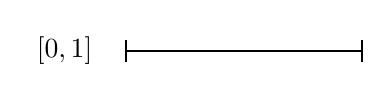
\begin{tikzpicture}[baseline=(current bounding box.center)]
\node[anchor=east] at (-.3,0) {$[0,1]$};
\draw[thick] (0,0)--(3,0);
\draw[thick] (0,-.14)--(0,.14);
\draw[thick] (3,-.14)--(3,.14);
\end{tikzpicture}
\end{center}
— такая структура $\exists$ оператор.
\SourceFigure{GELFAND-P000088}{unit-interval}{Слева подпись $[0,1]$, затем отрезок с двумя концевыми штрихами. Ниже $(Vf)(x)=\int_0^x f(y)\,dy$.}
\begin{equation*}
(Vf)(x)=\int_0^x f(y)\,dy
\end{equation*}
(отв. в 50-х годах).
\underline{Гипотеза.} Мера на прямой $\mu$.
\begin{center}
\begin{tikzpicture}
\draw (0,0)--(4,0);
\node[below] at (0,0){$-\infty$};
\node[below] at (4,0){$+\infty$};
\end{tikzpicture}
\SourceFigure{GELFAND-P000088}{measure-line}{Под линией слева $-\infty$, справа $+\infty$.}
\end{center}
\begin{equation*}
\mu(x)=1,\qquad L^2(\mu).
\end{equation*}
[Сверху над первым аргументом: $(x)$.]
\Unclear{GELFAND-P000088}{measure-normalization}{Видна запись $\mu(x)=1$ и ещё $(x)$ сверху; $\mu$ / $M$. Под первой буквой отдельный короткий знак: $2$ / неразобранный знак.}
\begin{equation*}
(Af)(x)=\int_0^x f(y)\,d\mu(y).
\end{equation*}
\Unclear{GELFAND-P000088}{integral-origin}{Нижний предел виден как $0$.}
Возможно, структ. по инв. подпр. изоморфна $\operatorname{supp}\mu$.
\Unclear{GELFAND-P000088}{support-letter}{В $L^2(\mu)$ и после $\operatorname{supp}$ буква $\mu$ / $M$.}



\Needspace{5\baselineskip}
\SourcePage{GELFAND-P000089}{61}
\underline{Возможный контрпример.}
$X$ — пр-во с мерой $\mu$.
$T$ — преобр., сохр. меру (по русски дин. система).
$\varphi$ — огр. ф-я.
[Зачёркнуто перед формулой:
Опер. / неразборчиво.]
\Unclear{GELFAND-P000089}{operator-cancel}{Опер. / неразборчиво}
[Над формулой: в $L^2$.]
\begin{equation*}
(Af)(x)=\varphi(x)f(Tx).
\end{equation*}
\SourceFigure{GELFAND-P000089}{weighted-formula}{Вверху $X,T,\varphi$; над формулой «в $L^2$»; справа $f(Tx)$.}
$\exists$ примеры преобр. с простым непр. спектром.
\begin{center}
\begin{tikzpicture}
\draw (0,0)--(3,0);
\draw (0,-0.12)--(0,0.12);
\draw (3,-0.12)--(3,0.12);
\node[below] at (0,0){$0$};
\node[below] at (3,0){$1$};
\end{tikzpicture}
\end{center}
\begin{gather*}
Tx=x+\alpha\pmod1,\qquad\alpha\text{ — иррац.}\\
\varphi(x)=x.
\end{gather*}
\SourceFigure{GELFAND-P000089}{interval-rotation}{Отрезок с двумя концевыми штрихами, подписи $0$, $1$ снизу. Справа $Tx=x+\alpha\pmod1$, «$\alpha$ — иррац.», затем $\varphi(x)=x$.}
\begin{quote}
\begin{tabular}{||l}
Изучить подробно\\
\uwave{этот оператор}
\end{tabular}
\end{quote}
\SourceFigure{GELFAND-P000089}{study-emphasis}{В правом поле две вертикальные черты; волнистая линия под «этот оператор».}
Предположение:
[Зачёркнуто:
на один… / на дан… / неразборчиво.]

нет инв. подпр. ($\forall$ вектор циклич.).
\Unclear{GELFAND-P000089}{conjecture-cancel}{на один… / на дан… / неразборчиво}
На самом деле неизв. ни одного циклич. вектора.
\SourceFigure{GELFAND-P000089}{cyclic-assertions}{В скобках $\forall$ вектор циклич.; ниже «неизв. ни одного циклич. вектора».}
$\exists$ пример. опер. $A$ в $L^2(0,1)$ (Ornstein), близкий к
опер. без инв. подпр.
$\forall$ вектор $\in L^{2+\varepsilon}$ циклический (!).
\SourceFigure{GELFAND-P000089}{Ornstein}{В первой строке $L^2(0,1)$ и имя Ornstein; ниже $\forall$, $\in L^{2+\varepsilon}$ и $(!)$.}
(Преобр., для к-ро лебег. мера квазиинв. — мера $0$ в меру $0$ —
но инв. меры не существует.)
\SourceFigure{GELFAND-P000089}{quasi-invariance}{«мера $0$ в меру $0$»; после переноса «но инв. меры не существует».}
\begin{center}— $\bullet$ —\end{center}
\underline{Вопр. Гельфанда}: зачем нужны инв. подпр-ва и чем их можно заменить?
\SourceFigure{GELFAND-P000089}{Gelfand-question}{Подчёркнуты «Вопр. Гельфанда»; до и после вопроса разделители с точкой между двумя линиями.}
\begin{center}— $\bullet$ —\end{center}
Ещё один профессор, говорящий по английски (на F)
(венгр из Румынии), типа
Фойтш / Фойши
\Unclear{GELFAND-P000089}{surname-f}{Фойтш / Фойши}
[Густо переписана повторная запись:
ойши / Фойши / неразборчиво.]
\Unclear{GELFAND-P000089}{surname-cancel}{ойши / Фойши / неразборчиво}
\begin{gather*}
E,\qquad|\lambda|<1,\qquad \mathord{\tikz[baseline=(h.base)]{\node[draw,circle,inner sep=.7pt] (h) {$H$};}}(\lambda):E\longrightarrow E_*,\\
\|H(\lambda)\|\leq1.
\end{gather*}
\SourceFigure{GELFAND-P000089}{contraction-math}{Отдельно $E$; $|\lambda|<1$; первая буква $H$ обведена, у правого $E$ звёздочка внизу; ниже $\|H(\lambda)\|\leq1$.}
[Буква $H$ в первой записи обведена.]
Аналит. в сильной опер. топ. (аналит. сжатие).
\begin{equation*}
\{E,E_*,\mathord{\tikz[baseline=(h.base)]{\node[draw,circle,inner sep=.7pt] (h) {$H$};}}\}
\end{equation*}
[Последняя буква в тройке обведена.]
\Unclear{GELFAND-P000089}{tuple-letter}{В тройке обведённый знак: $H$ / $\Theta$ / неразборчиво; выше обведённое $H$ имеет два ясных вертикальных штриха.}
Пр-во ф-й со знач. в исх. гильб. пр-ве $E$.
$L^2(E)$ — $L^2$ на окр. $2\pi$.
\SourceFigure{GELFAND-P000089}{Hardy-space}{В верхней строке гильб. пр-во $E$; затем $L^2(E)$, $2\pi$ и $H^2(E)$; в экспоненте $+int$.}
\begin{equation*}
H^2(E)\qquad\int_0 u(t)e^{int}\,dt=0,\qquad n=1,2,3,\ldots
\end{equation*}
\Unclear{GELFAND-P000089}{fourier-bound}{У интеграла ясно написан нижний $0$, верхний предел отдельно не виден.}
(граничные к аналит. ф-ям).
Не всё сделано в неконечномерном случае.
Инвар. афф. преобр. $A:H_1\longrightarrow H_2$,
\Unclear{GELFAND-P000089}{last-invariants}{Сокращение «афф.» / «дифф.»; ниже $H\to H$ и «жорданова форма».}
$H_1,H_2$ — конечномерны.
($H\to H$ — жорданова форма.)
Разные аналоги жорд. клеток.
\begin{equation*}
\int_0^x f(x)\,dx.
\end{equation*}
\SourceFigure{GELFAND-P000089}{final-integral}{Верхний предел $x$, нижний $0$; в подынтегральной записи и дифференциале тоже $x$.}



\Needspace{5\baselineskip}
\SourcePage{GELFAND-P000090}{unlabelled}
$20/\overline{\underline{\mathrm{IX}}}$.
\underline{Kohn.}\quad $\bar\partial$ — пробл. Неймана.
\begin{center}
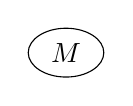
\begin{tikzpicture}
\node (m) at (0,0) {$M$};
\draw (0,0) ellipse (.48cm and .31cm);
\end{tikzpicture}
\end{center}
\SourceFigure{GELFAND-P000090}{opening-marks}{Дата $20/\mathrm{IX}$: черты сверху и снизу $\mathrm{IX}$; Kohn подчёркнуто; слева $M$ в овале.}
\begin{equation*}
M\subset C^n\qquad\text{огр. обл.}
\end{equation*}
\Unclear{GELFAND-P000090}{complex-dimension}{Показатель над $C$ густой: $n$ / $m$.}
\begin{equation*}
u_{\bar z_j}=\frac12(u_{x_j}+iu_{y_j})=\alpha_j.
\end{equation*}
\SourceFigure{GELFAND-P000090}{first-derivative}{В первом определении черта над $z_j$; справа $\frac12$, знак $+$ и $i$, затем $\alpha_j$.}
Даны $\alpha_j$, когда $\exists u$ и как оно зависит от $\alpha$.
Связь с класс. теорем.
\begin{gather*}
\bar\partial u=\alpha,\\
\sum u_{z_j}\,d\bar z_j=\sum\alpha_j\,d\bar z_j\\
\text{при усл. }\alpha_{j\bar z_k}=\alpha_{k\bar z_j}\qquad(\bar\partial\alpha=0).
\end{gather*}
\SourceFigure{GELFAND-P000090}{compatibility}{В дифференциалах черты над $z_j$; условие $\alpha_{j\bar z_k}=\alpha_{k\bar z_j}$, справа $(\bar\partial\alpha=0)$.}
\Unclear{GELFAND-P000090}{derivative-convention}{В сумме индекс $z_j$ без уверенно видимой черты; выше в определении ясно $\bar z_j$.}
\underline{Проблема Леви.}
\SourceFigure{GELFAND-P000090}{Levi-heading}{Заглавие подчёркнуто прямой линией; в вопросе $p$, $M$, знак $\exists$ и сокращения.}
Дано $p\in\partial M$ (гран.),
[Зачёркнуто:
какая / неразборчиво.]

$\exists$ голом. ф-я в $M$, к-рая не продолж. за точку $p$? Сущ.
\Unclear{GELFAND-P000090}{levi-problem-cancel}{какая / неразборчиво}
\uwave{Классич. теор. Леви реш. эту прбл. локально:}
\SourceFigure{GELFAND-P000090}{Levi-emphasis}{Под всей строкой от «Классич.» до «локально:» волнистая линия.}
$\underset{\substack{x\\0}}{r}$ — ур-е границы.
\begin{center}
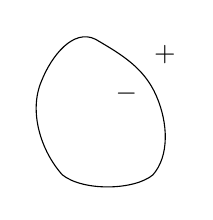
\begin{tikzpicture}[x=.014cm,y=-.014cm]
\draw (65,10) .. controls (45,0) and (25,25) .. (16,48)
 .. controls (4,76) and (16,112) .. (35,133)
 .. controls (54,148) and (100,147) .. (117,133)
 .. controls (132,116) and (131,86) .. (120,61)
 .. controls (109,36) and (89,24) .. (65,10) -- cycle;
\node at (93,59) {$-$};
\node at (128,24) {$+$};
\end{tikzpicture}
\end{center}
\SourceFigure{GELFAND-P000090}{boundary-signs}{Замкнутая неровная кривая, $-$ внутри и $+$ снаружи сверху справа. Под $r$ малый перекрещенный знак, похожий на $x$, затем $0$; точное чтение и роль этих знаков не установлены.}
\begin{equation*}
\underline{dr\neq0}
\end{equation*}
\SourceFigure{GELFAND-P000090}{nonzero-differential}{Запись $dr\neq0$ подчёркнута прямой линией; ниже «(точка неособая)».}
(точка неособая).
В т. $p\in\partial M$
\begin{equation*}
\sum r_{z_i}(p)a^i=0\qquad\text{гиперпл.}
\end{equation*}
\SourceFigure{GELFAND-P000090}{tangent-hyperplane}{Над формулой «В т. $p\in\partial M$»; в формуле $a^i$ и $=0$; справа «гиперпл.».}
\begin{equation*}
\sum r_{z_i\bar z_j}(p)a^i\bar a^j
\end{equation*}
— форма Леви.
\Unclear{GELFAND-P000090}{boundary-notation}{Буква функции границы похожа на $r$ / $\tau$, знак границы на $\partial$ / $b$.}
Если она полож. опр. на указ. гиперплоскости,

то сущ. в окр. т. $p$
[Зачёркнуто:
неразборчиво.]

ф-я, не прод. за точку $p$.
\Unclear{GELFAND-P000090}{local-cancel}{неразборчиво}
\SourceFigure{GELFAND-P000090}{Levi-positive}{Сокращения «полож. опр.», «на указ. гиперплоскости», затем «сущ. в окр. т. $p$».}
($\exists$ полином $W$, такой что нули расп. так:
\begin{center}
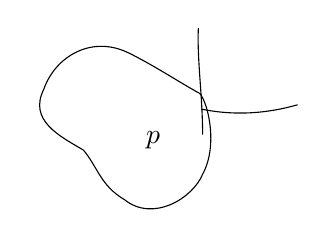
\begin{tikzpicture}[x=.018cm,y=-.018cm]
\draw (73,18) .. controls (46,4) and (20,20) .. (12,43)
 .. controls (1,65) and (23,76) .. (40,86)
 .. controls (50,98) and (52,111) .. (69,121)
 .. controls (89,137) and (117,120) .. (124,103)
 .. controls (135,83) and (128,53) .. (122,46)
 .. controls (109,39) and (91,27) .. (73,18) -- cycle;
\draw (121,0) .. controls (120,22) and (124,48) .. (124,75);
\draw (123,57) .. controls (147,62) and (170,60) .. (191,54);
\node at (89,79) {$p$};
\end{tikzpicture}
\end{center}
)
\SourceFigure{GELFAND-P000090}{local-w-geometry}{Замкнутая неровная кривая; у правого края почти вертикальный штрих и уходящий вправо штрих. Подпись $p$ внутри слева и ниже места их соединения. Точное положение густых перекрывающихся штрихов не установлено.}
Хороший ответ на ту зад. ($\bar\partial$) прив. к глоб. реш. пробл. Леви.
Пусть $\bar\partial$-прбл. разрешима для обл. $M$
($\forall\alpha$, $\bar\partial\alpha=0$, $\exists u$, $\bar\partial u=\alpha$).
Пусть
\begin{equation*}
g=\begin{cases}1&\text{в окр. }p,\\0&\text{вне }U\end{cases}
\end{equation*}
— срез. ф-я.
\SourceFigure{GELFAND-P000090}{cutoff-values}{В записи $g$ фигурная скобка, $1$ «в окр. $p$», $0$ «вне $U$»; справа «срез. ф-я».}
Обозн. $\alpha=\bar\partial\left(\frac gW\right)$.
$W$ — ранее постр. многочлен.
$\alpha$ — гладкая вплоть до границы.
\SourceFigure{GELFAND-P000090}{cutoff-alpha}{Слева $\alpha=\bar\partial(g/W)$; справа $W$ — ранее постр. многочлен; ниже «гладкая вплоть до границы».}
\begin{center}
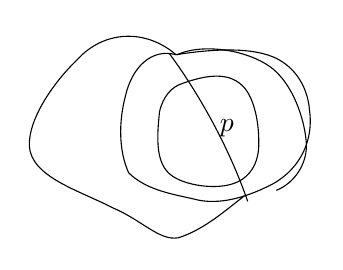
\begin{tikzpicture}[x=.014cm,y=-.014cm]
\draw (149,25) .. controls (121,1) and (83,3) .. (59,30)
 .. controls (40,48) and (15,82) .. (16,108)
 .. controls (18,136) and (61,148) .. (92,164)
 .. controls (118,175) and (134,194) .. (151,191)
 .. controls (174,184) and (194,166) .. (211,153);
\draw (150,25) .. controls (174,14) and (216,21) .. (237,38)
 .. controls (255,53) and (265,82) .. (267,103)
 .. controls (269,123) and (257,141) .. (240,148);
\draw (149,25) .. controls (127,19) and (109,36) .. (103,63)
 .. controls (97,86) and (97,112) .. (106,132)
 .. controls (123,149) and (150,152) .. (170,157)
 .. controls (192,161) and (216,153) .. (237,142)
 .. controls (262,128) and (274,102) .. (270,75)
 .. controls (268,51) and (254,34) .. (237,27)
 .. controls (213,17) and (174,21) .. (149,25) -- cycle;
\draw (155,51) .. controls (172,45) and (195,39) .. (209,53)
 .. controls (219,62) and (224,84) .. (224,103)
 .. controls (225,124) and (215,139) .. (197,143)
 .. controls (181,147) and (153,143) .. (142,132)
 .. controls (130,120) and (132,97) .. (134,77)
 .. controls (137,63) and (145,54) .. (155,51) -- cycle;
\draw (143,24) .. controls (168,58) and (196,106) .. (214,158);
\node at (195,92) {$p$};
\end{tikzpicture}
\end{center}
\SourceFigure{GELFAND-P000090}{cutoff-geometry}{Три неровных вложенных контура и наклонный штрих; во внешнем контуре снизу справа разрыв. $p$ внутри малого контура. Подписи $U$ или границы у контуров не видны; густые пересечения не вполне различимы.}
Решим ур-е к-л., получим $u$, рассм. $h=u-\frac gW$.
\Unclear{GELFAND-P000090}{solution-h}{После «ур-е» сокращение «к-л.»; вторая буква густая, точное чтение не вполне установлено. Далее $u$, $h=u-\frac gW$.}
$h$ голом. (т. к. $\bar\partial=0$)
[Зачёркнут штрих:
стрелка / неразборчиво.]
\Unclear{GELFAND-P000090}{final-arrow-cancel}{стрелка / неразборчиво}
$u$ не продолжается.
\Unclear{GELFAND-P000090}{noncontinuation-letter}{Перед «не продолжается» видна буква $u$.}
Аналого / Аналогично
тоже можно, но там за точку продолж.
\Unclear{GELFAND-P000090}{analogo-word}{Аналого / Аналогично}
\begin{center}
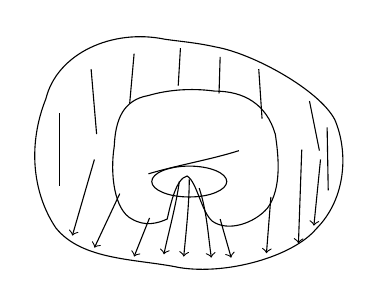
\begin{tikzpicture}[x=.014cm,y=-.014cm]
\draw (126,10) .. controls (78,0) and (28,23) .. (18,64)
 .. controls (2,104) and (5,148) .. (27,181)
 .. controls (51,211) and (101,209) .. (139,217)
 .. controls (182,224) and (242,207) .. (263,182)
 .. controls (291,154) and (292,111) .. (280,83)
 .. controls (266,56) and (206,23) .. (172,17)
 .. controls (154,13) and (140,12) .. (126,10) -- cycle;
\draw (111,61) .. controls (88,65) and (81,83) .. (80,107)
 .. controls (76,132) and (80,165) .. (96,173)
 .. controls (108,180) and (119,177) .. (128,173)
 .. controls (131,160) and (136,136) .. (146,134)
 .. controls (155,139) and (159,167) .. (169,175)
 .. controls (183,185) and (207,177) .. (219,163)
 .. controls (232,145) and (229,116) .. (226,96)
 .. controls (218,69) and (198,57) .. (171,57)
 .. controls (149,54) and (128,56) .. (111,61) -- cycle;
\draw (148,139) ellipse (34 and 14);
\draw (111,132) .. controls (138,124) and (168,119) .. (193,111);
\draw (30,77)--(30,143);
\draw (59,37)--(64,96);
\draw (98,23)--(94,68);
\draw (140,18)--(138,52);
\draw (176,26)--(175,59);
\draw (211,37)--(214,82);
\draw (257,66)--(266,111);
\draw (273,90)--(274,147);
\draw[->] (62,119)--(42,188);
\draw[->] (85,150)--(62,199);
\draw[->] (112,172)--(98,207);
\draw[->] (139,139) .. controls (136,161) and (129,186) .. (125,205);
\draw[->] (148,137) .. controls (148,159) and (145,186) .. (143,207);
\draw[->] (157,145) .. controls (164,166) and (165,187) .. (168,208);
\draw[->] (176,173)--(186,208);
\draw[->] (222,153)--(218,204);
\draw[->] (250,110)--(247,195);
\draw[->] (267,119)--(261,179);
\end{tikzpicture}
\end{center}
\SourceFigure{GELFAND-P000090}{global-geometry}{Внешний контур; внутренний контур с выемкой снизу; штриховка между ними. У выемки малый овал и косой штрих над ним; несколько длинных штрихов со стрелками вниз. Густые пересечения и отдельные концы штрихов не вполне различимы.}
[Зачёркнуто справа от рисунка:
неразборчиво.]
\Unclear{GELFAND-P000090}{figure-cancel}{неразборчиво}
Нужно учт. геом. структуру в целом всей области.
\SourceFigure{GELFAND-P000090}{whole-domain}{Последняя фраза переносится на «области.»; выше «но там за точку продолж.».}


\Needspace{5\baselineskip}
\begin{GelfandAdjacentEvidence}{GELFAND-P000091}{1}
\SourcePage{GELFAND-P000091}{62}
$a^{p,q}$ — пр-во форм типа $p,q$.
\SourceFigure{GELFAND-P000091}{opening-type}{$a^{p,q}$; «пр-во форм типа $p,q$».}
\end{GelfandAdjacentEvidence}
\begin{GelfandAdjacentEvidence}{GELFAND-P000091}{2}

\begin{equation*}
a^{p,q-1}\underset{\tikz[baseline=(e.base)]{\node[draw,ellipse,inner sep=1pt] (e) {$\text{ур-е}$};}}{\overset{\bar\partial}{\longrightarrow}}
a^{p,q}\overset{\bar\partial}{\longrightarrow}\alpha^{p,q+1}.
\end{equation*}
\SourceFigure{GELFAND-P000091}{dolbeault-chain}{Две стрелки с $\bar\partial$; под первой обведено «ур-е».}
\Unclear{GELFAND-P000091}{forms-space-letter}{Начальная и средняя буквы имеют облик $a$, последняя в цепочке и следующая запись — $\alpha$; различие $a/\alpha$ оставлено по месту.}
\end{GelfandAdjacentEvidence}
\begin{GelfandAdjacentEvidence}{GELFAND-P000091}{3}

Общие теоремы. $\alpha^{p,q}$ — гильб. скал. произв.
$\varphi,\psi\in D_{\bar\partial^*}$.
\begin{equation*}
Q(\varphi,\psi)=(\bar\partial\varphi,\bar\partial\psi)
+(\bar\partial^*\varphi,\bar\partial^*\psi).
\end{equation*}
[Справа:] ($\bar\partial$ на гладк. формах 1-й степ. без гр. условий).
\SourceFigure{GELFAND-P000091}{Q-form}{$D_{\bar\partial^*}$, два слагаемых в $Q(\varphi,\psi)$; справа скобки о гладк. формах 1-й степ. без гр. условий.}
\end{GelfandAdjacentEvidence}
\begin{GelfandAdjacentEvidence}{GELFAND-P000091}{4}

\begin{center}
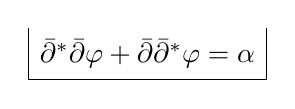
\begin{tikzpicture}
\node[inner sep=4pt] (op) {$\bar\partial^*\bar\partial\varphi+\bar\partial\bar\partial^*\varphi=\alpha$};
\draw (op.north west)--(op.south west)--(op.south east)--(op.north east);
\end{tikzpicture}
\end{center}
\SourceFigure{GELFAND-P000091}{boxed-operator}{Уравнение с двумя слагаемыми и правой частью $\alpha$; рамка слева, снизу и справа, без верхней стороны.}
\end{GelfandAdjacentEvidence}
\begin{GelfandAdjacentEvidence}{GELFAND-P000091}{5}

С пом. полож. опр. зад. [Зачёркнуто: неразборчиво] большего пор. реш. зад. 1-го пор.
\Unclear{GELFAND-P000091}{positive-problem-cancel}{После «зад.» густо зачёркнуто прежнее краткое выражение; начальный 1-/4-подобный штрих, остальная запись неразборчива.}
\end{GelfandAdjacentEvidence}
\begin{GelfandAdjacentEvidence}{GELFAND-P000091}{6}

Но здесь исп., что сист. 1-го пор. и усл. разреш. 1-го пор.
(По общ. переопр. сист. $\exists$ раб. Спенсера.)
Связ. с нейман. зад.
\SourceFigure{GELFAND-P000091}{first-order-argument}{«сист. 1-го пор.», «усл. разреш. 1-го пор.»; в скобках $\exists$ раб. Спенсера; затем связь с нейман. зад.}
\end{GelfandAdjacentEvidence}
\begin{GelfandAdjacentEvidence}{GELFAND-P000091}{7}

Апр. оц.
\begin{equation*}
\int_{\partial M}|\varphi|^2\,dS\le C Q(\varphi,\varphi)
\qquad\forall\varphi\in D_{\bar\partial^*}\cap\alpha^{p,q}.
\end{equation*}
\SourceFigure{GELFAND-P000091}{apriori-estimate}{У интеграла $\partial M$, подынтегрально $|\varphi|^2dS$; $\le C Q(\varphi,\varphi)$ и $\forall\varphi\in D_{\bar\partial^*}\cap\alpha^{p,q}$.}
\end{GelfandAdjacentEvidence}
\begin{GelfandAdjacentEvidence}{GELFAND-P000091}{8}

(но не мин. $\sum$ кв. 1-х произв., $n=1\sim\int$ Дирихле).
\SourceFigure{GELFAND-P000091}{Dirichlet-comparison}{Перед $\sum$ написано «мин.»; далее «кв. 1-х произв.», $n=1\sim\int$ Дирихле.}
\end{GelfandAdjacentEvidence}
\begin{GelfandAdjacentEvidence}{GELFAND-P000091}{9}

Попытка прим. проекции (лок.) нет, ни к чему не прив.
(Cohn 2 года зан. этим, $\int$ ур-я и т. д.)
Простейший случай нейман. задачи.
Cohn и Rossi Ann. Math. 1965 о голом. продолж. форм (!) внутрь обл.
\SourceFigure{GELFAND-P000091}{projection-and-Cohn}{«Попытка прим. проекции (лок.)»; Cohn в двух местах; «2 года», $\int$ ур-я; Rossi, Ann. Math. 1965; после «форм» стоит $(!)$.}
\end{GelfandAdjacentEvidence}
\begin{GelfandAdjacentEvidence}{GELFAND-P000091}{10}


\uwave{Планы на будущее}.
\SourceFigure{GELFAND-P000091}{plans-emphasis}{Волнистая линия под заголовком «Планы на будущее».}
\Unclear{GELFAND-P000091}{plans-title-correction}{Слово «на» в заголовке густо переписано; прежние штрихи неразборчивы.}
\end{GelfandAdjacentEvidence}
\begin{GelfandAdjacentEvidence}{GELFAND-P000091}{11}

\underline{Учить:} Винберг (алгебраические группы),
\SourceFigure{GELFAND-P000091}{study-heading}{«Учить:» подчёркнуто прямой линией; Винберг (алгебраические группы).}
\end{GelfandAdjacentEvidence}
\begin{GelfandAdjacentEvidence}{GELFAND-P000091}{12}

Атий[?] (…дробно[?]; начало в скобках густо переписано), алгебр. геометрия.

\Unclear{GELFAND-P000091}{atiyah-parenthesis}{Атий[?] (…дробно[?]; начало в скобках густо переписано), алгебр. геометрия.}
\end{GelfandAdjacentEvidence}
\begin{GelfandAdjacentEvidence}{GELFAND-P000091}{13}

читать в порядке ликбеза:
[Зачёркнуто:
G… / Г…; остальная часть имени неразборчива.
] и Rossi «ф-и многих компл. пер.» 1965
(пучки, когом. и т. п.).
\Unclear{GELFAND-P000091}{cancelled-book-name}{G… / Г…; остальная часть имени неразборчива.}
\SourceFigure{GELFAND-P000091}{reading-list}{После зачёркнутого имени «и Rossi»; «ф-и многих компл. пер.» 1965; в скобках «пучки, когом. и т. п.».}
\end{GelfandAdjacentEvidence}
\begin{GelfandAdjacentEvidence}{GELFAND-P000091}{14}

Обзор Дьёдонне о раб. Гротендика
(Ман. / Мат.[?] 9:1); сокращённое первое слово не вполне уверенное.

\Unclear{GELFAND-P000091}{review-volume}{(Ман. / Мат.[?] 9:1); сокращённое первое слово не вполне уверенное.}
\end{GelfandAdjacentEvidence}
\begin{GelfandAdjacentEvidence}{GELFAND-P000091}{15}


$\underline{27/\overline{\underline{\mathrm{IX}}}}$ \underline{Finn}. Идеи в теор. Гаусса-Бонне.
\SourceFigure{GELFAND-P000091}{Finn-heading}{Под датой и Finn отдельные прямые линии; над и под IX короткие черты.}
\end{GelfandAdjacentEvidence}
\begin{GelfandAdjacentEvidence}{GELFAND-P000091}{16}

Обобщ. Кон-Фоссена: пов. не замкнутая, а полная (напр., параболоид).
\SourceFigure{GELFAND-P000091}{Finn-surface-statement}{«пов. не замкнутая, а полная»; в скобках «напр., параболоид».}
\end{GelfandAdjacentEvidence}
\begin{GelfandAdjacentEvidence}{GELFAND-P000091}{17}

$C=2\pi$ [Зачёркнутый знак: неразборчиво]; $\chi=1$.
\Unclear{GELFAND-P000091}{finn-curvature-cancel}{После первого $C=2\pi$ густо зачёркнут знак; точное чтение не установлено.}
\end{GelfandAdjacentEvidence}
\begin{GelfandAdjacentEvidence}{GELFAND-P000091}{18}

\begin{center}
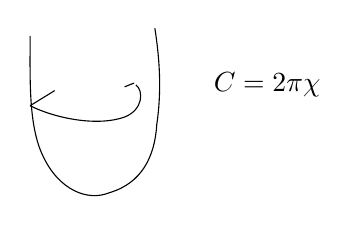
\begin{tikzpicture}[x=.024cm,y=-.024cm]
\draw (10,20) .. controls (10,43) and (9,68) .. (17,84)
 .. controls (25,101) and (40,108) .. (52,103)
 .. controls (69,98) and (76,84) .. (77,67)
 .. controls (80,47) and (78,29) .. (76,16);
\draw (10,57) .. controls (24,64) and (46,68) .. (60,63)
 .. controls (70,59) and (70,49) .. (66,46);
\draw (10,57)--(23,49);
\draw (60,47)--(65,45);
\node[anchor=west] at (102,46) {$C=2\pi\chi$};
\end{tikzpicture}
\qquad
\begin{tikzpicture}[x=.024cm,y=-.024cm]
\draw (0,0) .. controls (6,20) and (15,38) .. (30,49)
 .. controls (45,60) and (67,65) .. (88,63)
 .. controls (114,61) and (130,47) .. (138,29)
 .. controls (145,14) and (147,1) .. (146,-5);
\node[anchor=west] at (173,25) {$\chi=1$};
\node[anchor=west] at (135,93) {для неё $C<2\pi$};
\end{tikzpicture}
\end{center}
\SourceFigure{GELFAND-P000091}{finn-sections}{Две открытые вверх линии; у маленькой слева короткий изогнутый поперечный штрих с утолщёнными концами. Его точная роль и направление не установлены. Справа от неё $C=2\pi\chi$; у большой $\chi=1$, ниже «для неё $C<2\pi$».}
\end{GelfandAdjacentEvidence}
\begin{GelfandAdjacentEvidence}{GELFAND-P000091}{19}

($C=\int K\,dS$).
\SourceFigure{GELFAND-P000091}{curvature-integral}{$C=\int KdS$ заключено в круглые скобки.}
\end{GelfandAdjacentEvidence}
\begin{GelfandAdjacentEvidence}{GELFAND-P000091}{20}

Теор. Кон-Фоссена: $\forall$ полн. пов. $C\le2\pi\chi$.
\SourceFigure{GELFAND-P000091}{Finn-final-bound}{В последней строке $\forall$ полн. пов. и $C\le2\pi\chi$.}
\end{GelfandAdjacentEvidence}




\begin{GelfandAdjacentEvidence}{GELFAND-P000092}{1}
\SourcePage{GELFAND-P000092}{unlabelled}
Цель раб. — заменить нер-во равенством.
\SourceFigure{GELFAND-P000092}{opening-purpose}{«Цель раб. — заменить нер-во равенством».}
\end{GelfandAdjacentEvidence}
\begin{GelfandAdjacentEvidence}{GELFAND-P000092}{2}

В след. раз обзор
Волевича[?]

по вар., анал. рассл.
\Unclear{GELFAND-P000092}{reviewer-name}{Волевича[?]}
\end{GelfandAdjacentEvidence}
\begin{GelfandAdjacentEvidence}{GELFAND-P000092}{3}

$Kohn$'ом[?]

\Unclear{GELFAND-P000092}{next-review-name}{$Kohn$'ом[?]; густое начало имени и окончание после апострофа.}
\end{GelfandAdjacentEvidence}
\begin{GelfandAdjacentEvidence}{GELFAND-P000092}{4}


\underline{Гельфанд.}
[Зачёркнуто: Atiy…; окончание неразборчиво.] \underline{Atiyah.}

\Unclear{GELFAND-P000092}{atiyah-heading-cancel}{[Зачёркнуто: Atiy…; окончание неразборчиво.] \underline{Atiyah.}}
\end{GelfandAdjacentEvidence}
\begin{GelfandAdjacentEvidence}{GELFAND-P000092}{5}

\uwave{Теоремы о неподвижных точках.}
\SourceFigure{GELFAND-P000092}{heading-emphasis}{Прямые линии под «Гельфанд.» и «Atiyah.»; волнистая линия под «Теоремы о неподвижных точках».}
\end{GelfandAdjacentEvidence}
\begin{GelfandAdjacentEvidence}{GELFAND-P000092}{6}

(сод. теор. Брауэра, ф-лу Лефшица, теор. о том, что лин. пр. им. соб. вектор,
теор. Вейля о следах предст. и т. п.)
\SourceFigure{GELFAND-P000092}{fixedpoint-examples}{В начале скобок «сод.»; далее теор. Брауэра, ф-ла Лефшица, соб. вектор, теор. Вейля о следах предст.}
\end{GelfandAdjacentEvidence}
\begin{GelfandAdjacentEvidence}{GELFAND-P000092}{7}

$X$ — дифф. многообр. и на нём $n$ вект. рассл. $E_1,\ldots,E_n$.
$\Gamma(E_i)$ — сечения $E_i$. (кажд. рассл. — свою разм.)
\SourceFigure{GELFAND-P000092}{bundle-sections}{$X$, $n$, $E_1,\ldots,E_n$ и $\Gamma(E_i)$; в скобках «кажд. рассл. — свою разм.», последнее окончание в «свою» тесное.}
\end{GelfandAdjacentEvidence}
\begin{GelfandAdjacentEvidence}{GELFAND-P000092}{8}

\underline{Пример:} $X\times I$ ($I$ — прямая). Пр-во функций.
\SourceFigure{GELFAND-P000092}{trivial-bundle}{Прямое подчёркивание «Пример:»; $X\times I$, $I$ — прямая, «Пр-во функций».}
\end{GelfandAdjacentEvidence}
\begin{GelfandAdjacentEvidence}{GELFAND-P000092}{9}

\uwave{Эллиптический комплекс} (обобщ. элл. дифф. операторы).
\SourceFigure{GELFAND-P000092}{elliptic-heading}{Волнистая линия под «Эллиптический комплекс»; далее «обобщ. элл. дифф. операторы».}
\end{GelfandAdjacentEvidence}
\begin{GelfandAdjacentEvidence}{GELFAND-P000092}{10}

\begin{equation*}
\Gamma(E_1)\overset d\longrightarrow\Gamma(E_2)\overset d\longrightarrow
\cdots\overset d\longrightarrow\Gamma(E_n).
\end{equation*}
послед. линейных отображений, таких, что $1^\circ\ d^2=0$.
\SourceFigure{GELFAND-P000092}{differential-chain}{Три стрелки с $d$; $\Gamma(E_1)$, $\Gamma(E_2)$, многоточие, $\Gamma(E_n)$; $1^\circ$, $d^2=0$.}
\end{GelfandAdjacentEvidence}
\begin{GelfandAdjacentEvidence}{GELFAND-P000092}{11}

$2^\circ$. Рассм. $e\in E_{i,x_0}$, $s(x)\in\Gamma(E_i)$, что $s(x_0)=e$.
Пусть $f(x)$ — функция, обращ. в $0$ в точке $x_0$.
Рассм. $d(f^m s(x))=s_1(x)\in\Gamma(E_{i+1})$.
\SourceFigure{GELFAND-P000092}{differential-condition}{$e\in E_{i,x_0}$; $s(x_0)=e$; функция $f(x)$ обращ. в $0$ в $x_0$; $d(f^m s(x))=s_1(x)\in\Gamma(E_{i+1})$.}
\end{GelfandAdjacentEvidence}
\begin{GelfandAdjacentEvidence}{GELFAND-P000092}{12}

Тогда, если
[Зачёркнуто: $\exists$ с неразборчивым продолжением.] $\exists m$,

что $\forall x_0$ ($f(x_0)=0$) $s_1(x_0)$ зависит лишь от 1-х дифференциалов $f$
в точке $x_0$, то опер. наз. диффер.
($\exists m$, что $\forall f$, $\forall x_0$, $\forall s$ и т. д.)
наименьшее $m$ наз. порядком дифф. опер. что $s(x_0)=e$.
(В окр. точки это лок. дифф. оператор.)
\Unclear{GELFAND-P000092}{m-condition-cancel}{[Зачёркнуто: $\exists$ с неразборчивым продолжением.] $\exists m$,}
\SourceFigure{GELFAND-P000092}{least-order}{Три знака $\forall$ в скобках; «наименьшее $m$», затем «что $s(x_0)=e$»; в последней скобке «В окр. точки».}
\end{GelfandAdjacentEvidence}
\begin{GelfandAdjacentEvidence}{GELFAND-P000092}{13}

\begin{equation*}df=(\eta,dx).\end{equation*}
$df$ — [Зачёркнуто краткое слово: неразборчиво] вект.; $\eta$ — градиент (из [«кас.» вставлено сверху над густо переписанными штрихами] пр-ва).

$\eta\in T_x^*$.
\Unclear{GELFAND-P000092}{gradient-corrections}{$df$ — [Зачёркнуто краткое слово: неразборчиво] вект.; $\eta$ — градиент (из [«кас.» вставлено сверху над густо переписанными штрихами] пр-ва).}
\SourceFigure{GELFAND-P000092}{covector-source}{$df=(\eta,dx)$; рядом $\eta$ — градиент; ниже $\eta\in T_x^*$.}
\end{GelfandAdjacentEvidence}
\begin{GelfandAdjacentEvidence}{GELFAND-P000092}{14}

\begin{equation*}\sigma(d,\eta)e\end{equation*}

— лин. ф-я $e$, наз. символом дифф. опер.
\Unclear{GELFAND-P000092}{symbol-operator-cancel}{Первый аргумент: $d$ дописано над густо отменённым знаком; прежний знак неразборчив.}
\end{GelfandAdjacentEvidence}
\begin{GelfandAdjacentEvidence}{GELFAND-P000092}{15}

\underline{Пример.} Опр. Лапл. $m=2$.
\begin{equation*}
\frac{\partial^2(f^2(x)s(x))}{\partial x^2}
=2\left(\frac{\partial f}{\partial x}\right)^2s(x).
\end{equation*}
\SourceFigure{GELFAND-P000092}{laplace-example}{Прямое подчёркивание «Пример.»; $m=2$; во второй производной $f^2(x)s(x)$, справа $2(\partial f/\partial x)^2s(x)$.}
\end{GelfandAdjacentEvidence}
\begin{GelfandAdjacentEvidence}{GELFAND-P000092}{16}

Символ $2(\eta_1^2+\eta_2^2+\cdots+\eta_n^2)$.
\SourceFigure{GELFAND-P000092}{principal-symbol}{Множитель $2$; $\eta_1^2+\eta_2^2+\cdots+\eta_n^2$.}
\end{GelfandAdjacentEvidence}
\begin{GelfandAdjacentEvidence}{GELFAND-P000092}{17}

Рассм.
\begin{equation*}
0\longrightarrow E_{1,x_0}\overset{\sigma(\eta,d)}{\longrightarrow}E_{2,x_0}
\overset{\sigma(\eta,d)}{\longrightarrow}\cdots\longrightarrow E_{n,x_0}\longrightarrow0.
\end{equation*}
\SourceFigure{GELFAND-P000092}{symbol-sequence}{Нулевые концы; $E_{1,x_0}$, $E_{2,x_0}$, многоточие, $E_{n,x_0}$; над первыми двумя стрелками $\sigma(\eta,d)$.}
\end{GelfandAdjacentEvidence}
\begin{GelfandAdjacentEvidence}{GELFAND-P000092}{18}

Комплекс эллиптический, если $\forall\eta\ne0$ эта послед. точна.
\SourceFigure{GELFAND-P000092}{elliptic-exactness}{В последней строке $\forall\eta\ne0$ и «эта послед. точна».}
\end{GelfandAdjacentEvidence}




\begin{GelfandAdjacentEvidence}{GELFAND-P000093}{1}
\SourcePage{GELFAND-P000093}{63}
\underline{Примеры.} $1)$ $X$ — обл. в $R^n$.
пучок $1$ ($X\times R$).
\SourceFigure{GELFAND-P000093}{opening-examples}{Прямое подчёркивание «Примеры.»; $1)$, $X$, $R^n$, пучок $1$, $X\times R$.}
\end{GelfandAdjacentEvidence}
\begin{GelfandAdjacentEvidence}{GELFAND-P000093}{2}

\begin{equation*}-\Gamma(1)\overset\Delta\longrightarrow\Gamma(1).\end{equation*}
опр. Лапласа.
\Unclear{GELFAND-P000093}{first-example-minus}{Перед первой $\Gamma(1)$ короткий горизонтальный штрих: минус / тире.}
\end{GelfandAdjacentEvidence}
\begin{GelfandAdjacentEvidence}{GELFAND-P000093}{3}

$2)$ комплекс де Рама.
\SourceFigure{GELFAND-P000093}{de-rham-heading}{$2)$ комплекс де Рама.}
\end{GelfandAdjacentEvidence}
\begin{GelfandAdjacentEvidence}{GELFAND-P000093}{4}

\begin{equation*}T^*\wedge T^*\wedge\cdots\wedge T^*=\Lambda^{k}\,[?].\end{equation*}
\Unclear{GELFAND-P000093}{exterior-power}{Сама $\Lambda$ густо переписана; маленький показатель $k$[?], также $n$- / $x$- / $\kappa$-подобный.}
\end{GelfandAdjacentEvidence}
\begin{GelfandAdjacentEvidence}{GELFAND-P000093}{5}

$T$ —
[Начало слова густо переписано; прежние буквы неразборчивы] кас. пр-во.

\Unclear{GELFAND-P000093}{tangent-word-cancel}{[Начало слова густо переписано; прежние буквы неразборчивы] кас. пр-во.}
\end{GelfandAdjacentEvidence}
\begin{GelfandAdjacentEvidence}{GELFAND-P000093}{6}

$X$ — многообр. $T_x$ — кас. пр-во в точке $x$,
\SourceFigure{GELFAND-P000093}{tangent-space}{$X$ — многообр.; $T_x$ — кас. пр-во в точке $x$.}
\Unclear{GELFAND-P000093}{tangent-side-cancel}{[Справа: зачёркнута компактная запись; Т-/Ф-подобные штрихи, точное чтение не установлено.]}
\end{GelfandAdjacentEvidence}
\begin{GelfandAdjacentEvidence}{GELFAND-P000093}{7}

\begin{equation*}
\Gamma(\Lambda^0)\overset d\longrightarrow\Gamma(\Lambda^1)
\overset d\longrightarrow\cdots\overset d\longrightarrow\Gamma(\Lambda^n).
\end{equation*}
\Unclear{GELFAND-P000093}{de-rham-chain-cancels}{[Перед первой $\Gamma(\Lambda^0)$ густо отменены знаки, слева отдельный короткий штрих; после $\Gamma(\Lambda^n)$ зачёркнуты стрелка и $0$-подобный знак.]}
\end{GelfandAdjacentEvidence}
\begin{GelfandAdjacentEvidence}{GELFAND-P000093}{8}

[Справа:] сеч. — \uwave{дифф. формы.}
\SourceFigure{GELFAND-P000093}{sections-emphasis}{Справа «сеч. — дифф. формы.»; под «дифф. формы.» волнистая линия.}
\end{GelfandAdjacentEvidence}
\begin{GelfandAdjacentEvidence}{GELFAND-P000093}{9}

Символ на 1-м шагу — $(\eta_1,\ldots,\eta_n)$.
\begin{equation*}
d(s(x)f(x))=s(x_0)\eta=e\eta\qquad(df(x_0)=\eta).
\end{equation*}
\SourceFigure{GELFAND-P000093}{first-symbol}{На 1-м шагу $(\eta_1,\ldots,\eta_n)$; $s(x_0)\eta=e\eta$; в скобках $df(x_0)=\eta$.}
\end{GelfandAdjacentEvidence}
\begin{GelfandAdjacentEvidence}{GELFAND-P000093}{10}

В 2-м месте
\begin{equation*}
d(s(x)f(x))\big|_{x=x_0}
=s(x)\wedge df(x)\big|_{x=x_0}=e\wedge\eta.
\end{equation*}
\SourceFigure{GELFAND-P000093}{second-symbol}{Два ограничения $x=x_0$; $s(x)\wedge df(x)$ и $e\wedge\eta$.}
\end{GelfandAdjacentEvidence}
\begin{GelfandAdjacentEvidence}{GELFAND-P000093}{11}

(каждый символ дальше — умножение на $\eta$).
\SourceFigure{GELFAND-P000093}{multiplication-statement}{«каждый символ дальше — умножение на $\eta$» в скобках.}
\end{GelfandAdjacentEvidence}
\begin{GelfandAdjacentEvidence}{GELFAND-P000093}{12}

\uwave{Точность:} если $e\wedge\eta=0$, то $e=a\wedge\eta$.
\SourceFigure{GELFAND-P000093}{exactness-statement}{Волнистая линия под «Точность:»; $e\wedge\eta=0$, $e=a\wedge\eta$.}
\end{GelfandAdjacentEvidence}
\begin{GelfandAdjacentEvidence}{GELFAND-P000093}{13}

(миноры 2-го пор. $=0$, тогда векторы прям.
[Зачёркнуты заключительные знаки; густая запись, стрелка и $0$-подобный конец; точное чтение не установлено.]

)
\Unclear{GELFAND-P000093}{nilpotent-ending-cancel}{[Зачёркнуты заключительные знаки; густая запись, стрелка и $0$-подобный конец; точное чтение не установлено.]}
\end{GelfandAdjacentEvidence}
\begin{GelfandAdjacentEvidence}{GELFAND-P000093}{14}

$3)$ $\bar\partial$ и т. д.
\SourceFigure{GELFAND-P000093}{dolbeault-example}{$3)$; горизонтальная черта над $\partial$; «и т. д.».}
\end{GelfandAdjacentEvidence}
\begin{GelfandAdjacentEvidence}{GELFAND-P000093}{15}


$4/\overline{\underline{\mathrm{X}}}$ \uuline{Продолжение.} $\Gamma(E)$ — послед.
\SourceFigure{GELFAND-P000093}{continuation-date-heading}{Дата $4/\overline{\underline{\mathrm{X}}}$; «Продолжение.» подчёркнуто двумя прямыми линиями.}
\end{GelfandAdjacentEvidence}
\begin{GelfandAdjacentEvidence}{GELFAND-P000093}{16}

\begin{equation*}
d(f^m(x)s(x))\big|_{x_0}=\sigma(d,\eta)e,\qquad s(x_0)=e.
\end{equation*}
\SourceFigure{GELFAND-P000093}{operator-symbol}{$d(f^m(x)s(x))\big|_{x_0}=\sigma(d,\eta)e$; справа $s(x_0)=e$.}
\end{GelfandAdjacentEvidence}
\begin{GelfandAdjacentEvidence}{GELFAND-P000093}{17}

$\eta$ — 1-й дифференциал $f$.
$\eta\in T_{x_0}^*$.
\SourceFigure{GELFAND-P000093}{differential-covector}{Справа $s(x_0)=e$; $\eta$ — 1-й дифференциал $f$; $\eta\in T_{x_0}^*$.}
\end{GelfandAdjacentEvidence}
\begin{GelfandAdjacentEvidence}{GELFAND-P000093}{18}

Элл. опер. быв. не только диффер.
\SourceFigure{GELFAND-P000093}{elliptic-operators}{«Элл. опер. быв. не только диффер.»}
\Unclear{GELFAND-P000093}{endomorphism-heading-cancel}{[Перед заголовком зачёркнуто краткое слово; густые горизонтальные штрихи и нисходящий штрих; прежние буквы неразборчивы.]}
\end{GelfandAdjacentEvidence}
\begin{GelfandAdjacentEvidence}{GELFAND-P000093}{19}

\underline{Эндоморфизм комплекса.}
\SourceFigure{GELFAND-P000093}{endomorphism-heading}{Прямое подчёркивание «Эндоморфизм комплекса.»}
\end{GelfandAdjacentEvidence}
\begin{GelfandAdjacentEvidence}{GELFAND-P000093}{20}

\begin{equation*}
\Gamma(E_1)\longrightarrow\Gamma(E_2)\longrightarrow\cdots\longrightarrow\Gamma(E_n).
\end{equation*}
\SourceFigure{GELFAND-P000093}{endomorphism-chain}{$\Gamma(E_1)\longrightarrow\Gamma(E_2)\longrightarrow\cdots\longrightarrow\Gamma(E_n)$.}
\end{GelfandAdjacentEvidence}
\begin{GelfandAdjacentEvidence}{GELFAND-P000093}{21}

Оно индуцирует
[Перед «отобр.» густо отменён короткий знак / слово; неразборчиво.]

отобр.:
\begin{equation*}T_i^*:H^i(E)\longrightarrow H^i(E).\end{equation*}
\Unclear{GELFAND-P000093}{induced-map-cancel}{[Перед «отобр.» густо отменён короткий знак / слово; неразборчиво.]}
\SourceFigure{GELFAND-P000093}{induced-cohomology}{«Оно индуцирует … отобр.:»; $T_i^*:H^i(E)\longrightarrow H^i(E)$.}
\end{GelfandAdjacentEvidence}
\begin{GelfandAdjacentEvidence}{GELFAND-P000093}{22}

[Справа:] $T$ — эндом. комплекса,
$T_i:\Gamma(E_i)\to\Gamma(E_i)$, коммут. с $d$.
$(T_{i+1}d=dT_i)$.
$\swarrow$
\Unclear{GELFAND-P000093}{endomorphism-side-condition}{Справа наклонная стрелка пересекает окончание «комплекса» и проходит у стрелки между $\Gamma(E_i)$ и $\Gamma(E_i)$; её точная связь неясна. Формулы: $T_i:\Gamma(E_i)\to\Gamma(E_i)$, $(T_{i+1}d=dT_i)$.}
\end{GelfandAdjacentEvidence}
\begin{GelfandAdjacentEvidence}{GELFAND-P000093}{23}

Для элл. комплекса все они конечномерн.
(В случае элл. опер. оно им. разн. индекса.)
\SourceFigure{GELFAND-P000093}{finite-dimensional}{«все они конечномерн.»; в скобках «В случае элл. опер. оно им. разн. индекса».}
\end{GelfandAdjacentEvidence}
\begin{GelfandAdjacentEvidence}{GELFAND-P000093}{24}

В де Рамовом комплексе это обычные когом. с вещ. коэфф.
\SourceFigure{GELFAND-P000093}{de-rham-real-cohomology}{«В де Рамовом комплексе это обычные когом. с вещ. коэфф.»}
\end{GelfandAdjacentEvidence}
\begin{GelfandAdjacentEvidence}{GELFAND-P000093}{25}

\begin{equation*}
L(T,E)=\sum_{i=1}^{n}(-1)^i\operatorname{tr}(T_i^*).
\end{equation*}
\SourceFigure{GELFAND-P000093}{Lefschetz-formula}{$L(T,E)$; сумма от $i=1$ до $n$; $(-1)^i\operatorname{tr}(T_i^*)$.}
\end{GelfandAdjacentEvidence}
\begin{GelfandAdjacentEvidence}{GELFAND-P000093}{26}

[Под $L$:] число Лефшица гомологич.
[Справа:] $\Downarrow$ для де-рам. компл. это обычное число Лефшица.
[Внизу:] Лефшица-Атия-Ботта.
\SourceFigure{GELFAND-P000093}{Lefschetz-labels}{Под $L$: «число Лефшица гомологич.»; справа стрелка вниз с двумя штрихами и «для де-рам. компл. это обычное число Лефшица»; внизу «Лефшица-Атия-Ботта».}
\end{GelfandAdjacentEvidence}




\begin{GelfandAdjacentEvidence}{GELFAND-P000094}{1}
\SourcePage{GELFAND-P000094}{unlabelled}
Пусть $f:X\longrightarrow X$.
\SourceFigure{GELFAND-P000094}{opening-map}{«Пусть»; $f:X\longrightarrow X$.}
\end{GelfandAdjacentEvidence}
\begin{GelfandAdjacentEvidence}{GELFAND-P000094}{2}

Рассм.
\begin{equation*}
\psi_i:\Gamma(f^{-1}(E_i))\longrightarrow\Gamma(E_i).
\end{equation*}
\Unclear{GELFAND-P000094}{lift-maps}{У первого $\psi_i$ перед отчётливым $i$ густой дополнительный штрих; прежний индекс / знак неразборчив. В первой записи $\Gamma(f^{-1}(E_i))$, в повторной $\Gamma(f^{-1}E_i)$.}
\end{GelfandAdjacentEvidence}
\begin{GelfandAdjacentEvidence}{GELFAND-P000094}{3}

\underline{поднятие} — \sout{по отобр. пучков} $f$ по отобр. пучков.
\Unclear{GELFAND-P000094}{lifting-cancellations}{Зачёркнуто «по отобр. пучков», частично закрыто штрихами. Перед второй $\Gamma$ густо отменён короткий знак; точное чтение не установлено.}
\end{GelfandAdjacentEvidence}
\begin{GelfandAdjacentEvidence}{GELFAND-P000094}{4}

\begin{equation*}
\psi_i:\Gamma(f^{-1}E_i)\longrightarrow\Gamma(E_i),
\end{equation*}
\begin{equation*}
E_{i,f^{-1}x}\overset{\psi_{i,x}}{\longrightarrow}E_{i,x}.
\end{equation*}
\Unclear{GELFAND-P000094}{inverse-fibre-locator}{В индексе левого слоя видимое $f^{-1}x$.}
\end{GelfandAdjacentEvidence}
\begin{GelfandAdjacentEvidence}{GELFAND-P000094}{5}

Оно неоднозначн. опред. по $f$.
\SourceFigure{GELFAND-P000094}{lifting-nonunique}{«Оно неоднозначн. опред. по $f$».}
\end{GelfandAdjacentEvidence}
\begin{GelfandAdjacentEvidence}{GELFAND-P000094}{6}

Пучок де Рама: $f$ индуц. отобр. де Рам. пучков однозначно.
(естеств. поднятие).
\SourceFigure{GELFAND-P000094}{de-rham-lifting}{$f$ индуц. отобр. де Рам. пучков однозначно; в скобках «естеств. поднятие».}
\end{GelfandAdjacentEvidence}
\begin{GelfandAdjacentEvidence}{GELFAND-P000094}{7}

\begin{equation*}\boxed{f:X\longrightarrow X}.\end{equation*}
\SourceFigure{GELFAND-P000094}{map-frame}{Прямоугольная рамка вокруг $f:X\longrightarrow X$; скобка «естеств. поднятие» выше её верхней границы.}
\end{GelfandAdjacentEvidence}
\begin{GelfandAdjacentEvidence}{GELFAND-P000094}{8}

Предположим, что $f$ имеет лишь конечн. число изолир. неподв. точек
самой простой структуры.
\SourceFigure{GELFAND-P000094}{isolated-assumption}{«Предположим, что $f$ имеет лишь конечн. число изолир. неподв. точек самой простой структуры».}
\end{GelfandAdjacentEvidence}
\begin{GelfandAdjacentEvidence}{GELFAND-P000094}{9}

\uwave{Теор. Брауэра} для отрезка $[0,1]$. $f:x\to f(x)$.
\SourceFigure{GELFAND-P000094}{brouwer-heading}{Волнистая линия под «Теор. Брауэра»; $[0,1]$; $f:x\to f(x)$.}
\end{GelfandAdjacentEvidence}
\begin{GelfandAdjacentEvidence}{GELFAND-P000094}{10}

\begin{center}
\begin{tikzpicture}[x=1mm,y=1mm,line width=.5pt]
\draw (5,4)--(27,3.5)--(26,-14)--(5,-13)--cycle;
\draw (5,-12)--(26,3);
\draw (5,-8)--(9,-6)--(12,-4.5)--(16,-3.5)--(20,-3.8)--(23,-2)--(26,.2);
\node at (5,-18) {$0$};
\node at (26,-18) {$1$};
\node[anchor=north west,align=left,inner sep=0pt,text width=114mm] (fixedtext) at (35,5) {
$\rho$ — неподв. точка этого отображения.\par\smallskip
В ней у нас есть $\psi_i(\rho):$
[Зачёркнута $E$-подобная запись слоя; индексы неразборчивы.]
$E_{i,\rho}\to E_{i,\rho}$.\par\smallskip
В кас. \underline{пр-ве}\textsuperscript{$(x)$[?]} есть лин. преобразование.
};
\draw ([xshift=2mm,yshift=3mm]fixedtext.north east)
 --([xshift=-3mm,yshift=3mm]fixedtext.north west)
 --([xshift=-3mm,yshift=-2mm]fixedtext.south west)--++(-29mm,0);
\end{tikzpicture}
\end{center}
\SourceFigure{GELFAND-P000094}{brouwer-graph}{Прямоугольник с подписями $0$ и $1$, две восходящие линии, густое пересечение. Геометрия пересечения неясна. Угловая линия проходит сверху и слева от соседних строк о $\rho$, слое и касательном пространстве, затем уходит влево под рисунок.}
\SourceFigure{GELFAND-P000094}{fixed-point}{$\rho$ — неподв. точка этого отображения.}
\Unclear{GELFAND-P000094}{fixed-fibre-corrections}{Перед новым $E_{i,\rho}$ отменена $E$-подобная запись с неразобранными индексами. Над подчёркнутым «пр-ве» вставка $(x)$[?]; точная буква неуверенная.}
\end{GelfandAdjacentEvidence}
\begin{GelfandAdjacentEvidence}{GELFAND-P000094}{11}

Оно обозначается $J_\rho(f)$ в кас. пр-ве к $X$.
\SourceFigure{GELFAND-P000094}{tangent-J}{$J_\rho(f)$; «в кас. пр-ве к $X$».}
\end{GelfandAdjacentEvidence}
\begin{GelfandAdjacentEvidence}{GELFAND-P000094}{12}

Точка изолирована $\Leftarrow$ достаточно, чтобы было
\begin{equation*}\det(1-J_\rho(f))\ne0.\end{equation*}
(по теор. о неявных ф-ях).
\SourceFigure{GELFAND-P000094}{isolation-criterion}{Жирная стрелка влево $\Leftarrow$; $\det(1-J_\rho(f))\ne0$; «по теор. о неявных ф-ях».}
\end{GelfandAdjacentEvidence}
\begin{GelfandAdjacentEvidence}{GELFAND-P000094}{13}

Точка [зачёркнутое короткое слово неразборчиво] особая неподв., если он $0$, прав., если $\ne0$.
\Unclear{GELFAND-P000094}{regular-point-cancel}{После «Точка» густо отменено короткое слово; прежние буквы не восстанавливаются. Затем «особая неподв., если он $0$, прав., если $\ne0$».}
\end{GelfandAdjacentEvidence}
\begin{GelfandAdjacentEvidence}{GELFAND-P000094}{14}

Графики $(x,f(x))$ и $(x,x)$ пересек. трансверсально.
\SourceFigure{GELFAND-P000094}{transverse-graphs}{$(x,f(x))$ и $(x,x)$; «пересек. трансверсально».}
\end{GelfandAdjacentEvidence}
\begin{GelfandAdjacentEvidence}{GELFAND-P000094}{15}

Посмотрим число
\begin{equation*}
\frac{\operatorname{tr}\psi_i(\rho)}{|\det(1-J_\rho(f))|}.
\end{equation*}
\SourceFigure{GELFAND-P000094}{local-trace}{$\operatorname{tr}\psi_i(\rho)$ над $|\det(1-J_\rho(f))|$.}
\end{GelfandAdjacentEvidence}
\begin{GelfandAdjacentEvidence}{GELFAND-P000094}{16}

В т. $\rho$ есть $2$ лин. преобр. $\psi_i(\rho)$ — слой в себя,
и преобр. кас. пр-ва.
\SourceFigure{GELFAND-P000094}{two-maps}{В т. $\rho$ — $2$ лин. преобр.; $\psi_i(\rho)$ — слой в себя; преобр. кас. пр-ва.}
\end{GelfandAdjacentEvidence}
\begin{GelfandAdjacentEvidence}{GELFAND-P000094}{17}

\begin{equation*}
\sum(-1)^i\frac{\operatorname{tr}\psi_i(\rho)}{|\det(1-J_\rho(f))|}
=\sigma(\rho).
\end{equation*}
\SourceFigure{GELFAND-P000094}{local-contribution}{$\sum(-1)^i$ без видимых пределов; $\operatorname{tr}\psi_i(\rho)$; $|\det(1-J_\rho(f))|$; $\sigma(\rho)$.}
\end{GelfandAdjacentEvidence}
\begin{GelfandAdjacentEvidence}{GELFAND-P000094}{18}

Это число не зависит от комплекса, а зав. только от $f$ и индуц. отобр. в слоях
(но отобр. слоёв не произв., оно должно коммутировать с компл.).
\SourceFigure{GELFAND-P000094}{complex-independence}{«не зависит от комплекса»; $f$ и индуц. отобр. в слоях; в скобках «но отобр. слоёв не произв., оно должно коммутировать с компл.».}
\end{GelfandAdjacentEvidence}
\begin{GelfandAdjacentEvidence}{GELFAND-P000094}{19}

$\psi_i$ должно быть эндоморфизмом!
\SourceFigure{GELFAND-P000094}{endomorphism-warning}{$\psi_i$ должно быть эндоморфизмом!}
\end{GelfandAdjacentEvidence}




\begin{GelfandAdjacentEvidence}{GELFAND-P000095}{1}
\SourcePage{GELFAND-P000095}{64}
\underline{Теорема} Атия-Ботта.
\SourceFigure{GELFAND-P000095}{theorem-heading}{Подчёркнуто только «Теорема»; «Атия-Ботта»; номер $64$.}
\end{GelfandAdjacentEvidence}
\begin{GelfandAdjacentEvidence}{GELFAND-P000095}{2}

Пусть есть эллипт. комплекс $d$,
$f:X\to X$ и поднятие его $\psi$, являющееся эндоморфизмом
этого комплекса. Тогда имеет место ф-ла
\SourceFigure{GELFAND-P000095}{theorem-assumptions}{«эллипт. комплекс $d$»; $f:X\to X$; «поднятие его $\psi$, являющееся эндоморфизмом этого комплекса».}
\end{GelfandAdjacentEvidence}
\begin{GelfandAdjacentEvidence}{GELFAND-P000095}{3}

\begin{equation*}L(T,E)=\sum_\rho\sigma(\rho)\end{equation*}
по всем неподв. точкам.
\SourceFigure{GELFAND-P000095}{Lefschetz-local-formula}{$L(T,E)=\sum_\rho\sigma(\rho)$; «по всем неподв. точкам».}
\end{GelfandAdjacentEvidence}
\begin{GelfandAdjacentEvidence}{GELFAND-P000095}{4}

$T$ задаётся парой $f$ и $\psi$.
\SourceFigure{GELFAND-P000095}{T-pair}{$T$ задаётся парой $f$ и $\psi$.}
\end{GelfandAdjacentEvidence}
\begin{GelfandAdjacentEvidence}{GELFAND-P000095}{5}

\underline{Доказательство.}
\SourceFigure{GELFAND-P000095}{proof-heading}{Подчёркнуто «Доказательство».}
\end{GelfandAdjacentEvidence}
\begin{GelfandAdjacentEvidence}{GELFAND-P000095}{6}

Сначала нечётко[?] и неполно (идеи)
\Unclear{GELFAND-P000095}{proof-opening-word}{Первое слово после «Сначала»: «нечётко»[?] / «неточно»[?]; тесные средние штрихи.}
\end{GelfandAdjacentEvidence}
\begin{GelfandAdjacentEvidence}{GELFAND-P000095}{7}

$d:\Gamma(E)_i\longrightarrow\Gamma(E)_{i+1}$, по нему стр. новый оператор.
\SourceFigure{GELFAND-P000095}{initial-d-map}{$d:\Gamma(E)_i\longrightarrow\Gamma(E)_{i+1}$; индексы $i$, $i+1$ стоят вне скобок; «по нему стр. новый оператор».}
\end{GelfandAdjacentEvidence}
\begin{GelfandAdjacentEvidence}{GELFAND-P000095}{8}

Введём в $\Gamma(E)$ скалярное произведение.
\SourceFigure{GELFAND-P000095}{scalar-product}{Введём в $\Gamma(E)$ скалярное произведение.}
\end{GelfandAdjacentEvidence}
\begin{GelfandAdjacentEvidence}{GELFAND-P000095}{9}

Введём «опер. Лапласа»
\begin{equation*}\Box=d^*d+dd^*.\end{equation*}
\SourceFigure{GELFAND-P000095}{Laplacian}{«опер. Лапласа»; $\Box=d^*d+dd^*$.}
\end{GelfandAdjacentEvidence}
\begin{GelfandAdjacentEvidence}{GELFAND-P000095}{10}

Каждое $\Gamma(E)$ перев. в себя.
\SourceFigure{GELFAND-P000095}{degree-preservation}{«Каждое $\Gamma(E)$ перев. в себя».}
\end{GelfandAdjacentEvidence}
\begin{GelfandAdjacentEvidence}{GELFAND-P000095}{11}

Теорема Ходжа (обобщённая): $\Box$ им. дискр. положит.
спектр, каждому соб. числу соотв. кон. число соб. знач.
\SourceFigure{GELFAND-P000095}{Hodge-spectrum}{«дискр. положит. спектр»; «каждому соб. числу соотв. кон. число соб. знач.».}
\end{GelfandAdjacentEvidence}
\begin{GelfandAdjacentEvidence}{GELFAND-P000095}{12}

$\Gamma_\lambda(E_i)$ — подпр-во, ответ. соб. знач. $\lambda$. (соб. ф-и)
\SourceFigure{GELFAND-P000095}{eigenspace-definition}{$\Gamma_\lambda(E_i)$; «подпр-во, ответ. соб. знач. $\lambda$»; «соб. ф-и».}
\end{GelfandAdjacentEvidence}
\begin{GelfandAdjacentEvidence}{GELFAND-P000095}{13}

\begin{equation*}d:\Gamma_\lambda(E_i)\longrightarrow\Gamma_\lambda(E_{i+1}).\end{equation*}
\SourceFigure{GELFAND-P000095}{restricted-d-map}{$d:\Gamma_\lambda(E_i)\longrightarrow\Gamma_\lambda(E_{i+1})$.}
\end{GelfandAdjacentEvidence}
\begin{GelfandAdjacentEvidence}{GELFAND-P000095}{14}

\begin{center}
\begin{tikzpicture}[x=1mm,y=1mm,line width=.45pt]
\node at (0,0) {$\Box d=d\Box$};
\node at (18,.5) {\scriptsize $i$[?]};
\draw (1,0) ellipse (23mm and 6mm);
\end{tikzpicture}
\end{center}
\Unclear{GELFAND-P000095}{commutation-oval}{В овале $\Box d=d\Box$; справа от последнего квадрата отдельный малый $i$-подобный штрих[?].}
\end{GelfandAdjacentEvidence}
\begin{GelfandAdjacentEvidence}{GELFAND-P000095}{15}

\begin{equation*}
d:\Gamma(E_1)\longrightarrow\Gamma(E_2)\longrightarrow\cdots\longrightarrow\Gamma(E_n).
\end{equation*}
\SourceFigure{GELFAND-P000095}{full-complex}{$d:\Gamma(E_1)\to\Gamma(E_2)\to\cdots\to\Gamma(E_n)$.}
\end{GelfandAdjacentEvidence}
\begin{GelfandAdjacentEvidence}{GELFAND-P000095}{16}

Посмотрим теперь
\begin{equation*}
d:\Gamma_\lambda(E_1)\longrightarrow\Gamma_\lambda(E_2)\longrightarrow\cdots\longrightarrow\Gamma_\lambda(E_n).
\end{equation*}
\SourceFigure{GELFAND-P000095}{eigen-complex}{«Посмотрим теперь»; $d:\Gamma_\lambda(E_1)\to\Gamma_\lambda(E_2)\to\cdots\to\Gamma_\lambda(E_n)$.}
\end{GelfandAdjacentEvidence}
\begin{GelfandAdjacentEvidence}{GELFAND-P000095}{17}

$\Gamma_\lambda$ уже конечномерны ($d^2=0$), тоже возникают
гомологии.
\SourceFigure{GELFAND-P000095}{finite-dimensional}{$\Gamma_\lambda$ уже конечномерны; $(d^2=0)$; «тоже возникают гомологии».}
\end{GelfandAdjacentEvidence}
\begin{GelfandAdjacentEvidence}{GELFAND-P000095}{18}

\begin{equation*}
H^i\{\Gamma_\lambda(E)\}=\begin{cases}H^i(E),&\lambda=0,\\0,&\lambda\ne0.\end{cases}
\end{equation*}
\SourceFigure{GELFAND-P000095}{eigen-cohomology}{$H^i\{\Gamma_\lambda(E)\}$; $H^i(E)$ при $\lambda=0$, $0$ при $\lambda\ne0$.}
\end{GelfandAdjacentEvidence}
\begin{GelfandAdjacentEvidence}{GELFAND-P000095}{19}

(индексы есть только для дефин.[?] опер.)
\Unclear{GELFAND-P000095}{index-operator-abbreviation}{Сокращение после «для»: «дефин.»[?] / «диффин.»[?]; неразвёрнуто.}
\end{GelfandAdjacentEvidence}
\begin{GelfandAdjacentEvidence}{GELFAND-P000095}{20}

Для де Рам. компл. — теор. Ходжа — всякая [зачёркнутое выражение неразборчиво]
\SourceFigure{GELFAND-P000095}{de-rham-Hodge}{«Для де Рам. компл. — теор. Ходжа — всякая».}
\end{GelfandAdjacentEvidence}
\begin{GelfandAdjacentEvidence}{GELFAND-P000095}{21}

[Зачёркнутое выражение неразборчиво] замкн. форма
$\underset{\longrightarrow\,\longrightarrow}{\text{гомологична}}$ гармонической.
\Unclear{GELFAND-P000095}{harmonic-form-cancels}{Два густо зачёркнутых выражения: после «всякая» и перед «замкн.»; прежние буквы не установлены.}
\SourceFigure{GELFAND-P000095}{closed-form-statement}{«замкн. форма гомологична гармонической»; две короткие стрелки вправо под словом «гомологична».}
\end{GelfandAdjacentEvidence}
\begin{GelfandAdjacentEvidence}{GELFAND-P000095}{22}

Считать след: $\sum$ диаг. элем. $\equiv\sum$ соб. знач.
\SourceFigure{GELFAND-P000095}{trace-definition}{«Считать след»; $\sum$ диаг. элем. $\equiv\sum$ соб. знач.; три горизонтальные черты.}
\end{GelfandAdjacentEvidence}
\begin{GelfandAdjacentEvidence}{GELFAND-P000095}{23}

(1. След как $\int K(x,x)\,dx$, и $\sum$ следов в каждом подпр-ве
\SourceFigure{GELFAND-P000095}{kernel-trace}{$(1.$; «След как» $\int K(x,x)\,dx$; «и $\sum$ следов в каждом подпр-ве».}
\end{GelfandAdjacentEvidence}
\begin{GelfandAdjacentEvidence}{GELFAND-P000095}{24}

(инв. собств.)
\SourceFigure{GELFAND-P000095}{invariant-parenthesis}{В скобках «инв. собств.».}
\end{GelfandAdjacentEvidence}
\begin{GelfandAdjacentEvidence}{GELFAND-P000095}{25}

$\lambda\ne0$ [густо зачёркнут короткий знак, неразборчиво] следа нет, $\lambda=0$ счит. через гомологии. $\Bigg\}$[?]
\Unclear{GELFAND-P000095}{nonzero-trace-cancel}{После $\lambda\ne0$ густо отменён короткий знак / стрелка[?]. Читается «следа нет», затем «$\lambda=0$ счит. через гомологии». Справа крупный закрывающий скобкообразный знак: фигурная / круглая скобка[?].}
\end{GelfandAdjacentEvidence}




\begin{GelfandAdjacentEvidence}{GELFAND-P000096}{1}
\SourcePage{GELFAND-P000096}{unlabelled}
$11/\overline{\underline{\mathrm X}}$ \uwave{План} \uwave{семинара.}
\SourceFigure{GELFAND-P000096}{date-heading}{$11/\overline{\underline{\mathrm X}}$; верхняя и нижняя черты у $X$; «План» и «семинара» подчёркнуты волнисто.}
\end{GelfandAdjacentEvidence}
\begin{GelfandAdjacentEvidence}{GELFAND-P000096}{2}

1. Интегро-дифф. операторы (Агранович).
(2 часа)
\SourceFigure{GELFAND-P000096}{plan-operators}{Интегро-дифф. операторы; Агранович; ниже скобки «(2 часа)».}
\end{GelfandAdjacentEvidence}
\begin{GelfandAdjacentEvidence}{GELFAND-P000096}{3}

2. Атия-Зингер по индексу.
Кириллов или Гельфанд. Дынин.
(год. сем. Cartan-Schwartz
и сем. Вишика 64–65г.)
\SourceFigure{GELFAND-P000096}{plan-index}{Атия-Зингер по индексу; Кириллов или Гельфанд; Дынин; год. сем. Cartan-Schwartz и сем. Вишика $64$–$65$г.}
\end{GelfandAdjacentEvidence}
\begin{GelfandAdjacentEvidence}{GELFAND-P000096}{4}

3. Статистическая физика ($\underset{\text{Роберт Адльфович[?]}}{\text{Минлос}}$, 3 засед.).
\SourceFigure{GELFAND-P000096}{plan-physics}{Статистическая физика; Минлос; $3$ засед.; имя и отчество ниже фамилии.}
\Unclear{GELFAND-P000096}{minlos-patronymic}{Под «Минлос»: «Роберт Адльфович»[?] / «Роберт Адольфович»[?]; малая петля после «д» неуверенная.}
\end{GelfandAdjacentEvidence}
\begin{GelfandAdjacentEvidence}{GELFAND-P000096}{5}

4. Адели и группы аделей (Граев [зачёркнутый М-подобный знак, неразборчиво] Марк Иосифович).
(2 засед.)
\SourceFigure{GELFAND-P000096}{plan-adeles}{Адели и группы аделей; Граев Марк Иосифович; $(2$ засед.$)$.}
\Unclear{GELFAND-P000096}{graev-initial-cancel}{Между «Граев» и «Марк» густо отменён М-подобный знак; прежнее чтение не установлено.}
\end{GelfandAdjacentEvidence}
\begin{GelfandAdjacentEvidence}{GELFAND-P000096}{6}

5. Линейные алгебраические группы.
Кириллов
Гельфанд
\SourceFigure{GELFAND-P000096}{plan-groups}{Линейные алгебраические группы; справа столбиком Кириллов / Гельфанд.}
\end{GelfandAdjacentEvidence}
\begin{GelfandAdjacentEvidence}{GELFAND-P000096}{7}

6. Работа Ботта и Chern (Acta Math.) Гельфанд
Т. 114[?] $N=1$–$2$
\SourceFigure{GELFAND-P000096}{plan-bott-chern}{Работа Ботта и Chern; Acta Math.; Гельфанд; номер тома ниже названия журнала.}
\Unclear{GELFAND-P000096}{chern-volume-correction}{Густые знаки тома: «Т. 114»[?] / «Т. III»[?]; $N=1$–$2$. Ниже зачёркнут короткий знак / слово.}
\end{GelfandAdjacentEvidence}
\begin{GelfandAdjacentEvidence}{GELFAND-P000096}{8}

(перенос[?] теор. Неванлинны о нулях ф-й на [густо зачёркнутый фрагмент неразборчив] кривые
сеч. вект. пучков.)
\Unclear{GELFAND-P000096}{nevanlinna-cancel}{Первое слово в скобках «перенос»[?] / «перенес.»[?]. Перед «кривые» густо отменён фрагмент; затем «сеч. вект. пучков».}
\end{GelfandAdjacentEvidence}
\begin{GelfandAdjacentEvidence}{GELFAND-P000096}{9}

7. Теорема Рима\underline{на-Роха}-\underline{Гротен}дика. Каздан[?] Д. А.
\Unclear{GELFAND-P000096}{plan-riemann-roch}{Две прямые черты под частями названия: область «на-Роха» и начало «Гротендика»; точные границы неуверенные. Фамилия «Каздан»[?] / «Каждан»[?].}
\end{GelfandAdjacentEvidence}
\begin{GelfandAdjacentEvidence}{GELFAND-P000096}{10}

\uwave{Каздан[?].} Теор. Римана-Роха.
\Unclear{GELFAND-P000096}{kazhdan-heading}{Фамилия под волнистой чертой: «Каздан»[?] / «Каждан»[?]; густой знак между «а» и «д».}
\end{GelfandAdjacentEvidence}
\begin{GelfandAdjacentEvidence}{GELFAND-P000096}{11}

Вект. пучку соотв. класс когом. — класс Chern’а.
\SourceFigure{GELFAND-P000096}{Chern-class}{Вект. пучку соотв. класс когом.; класс Chern’а, латинская фамилия с русским окончанием.}
\end{GelfandAdjacentEvidence}
\begin{GelfandAdjacentEvidence}{GELFAND-P000096}{12}

\underline{Классы Черна.}
\SourceFigure{GELFAND-P000096}{Chern-heading}{Подчёркнуто «Классы Черна»; начало «Классы» написано густо.}
\end{GelfandAdjacentEvidence}
\begin{GelfandAdjacentEvidence}{GELFAND-P000096}{13}

$X$ — классич. алг. многообразие, афф. пр-во
\SourceFigure{GELFAND-P000096}{affine-space}{$X$ — классич. алг. многообразие, афф. пр-во.}
\end{GelfandAdjacentEvidence}
\begin{GelfandAdjacentEvidence}{GELFAND-P000096}{14}

алг. ф-и на нём — многочлены, это самое простое[?]
алг. многообразие.
\Unclear{GELFAND-P000096}{polynomial-functions}{«алг. ф-и на нём — многочлены»; «это самое простое»[?] / «это самое просто»[?]; окончание последнего слова густое; далее «алг. многообразие».}
\end{GelfandAdjacentEvidence}
\begin{GelfandAdjacentEvidence}{GELFAND-P000096}{15}

Аффинные алг. многообр. Пусть дан набор
многочленов
\begin{equation*}p_1(x_1,\ldots,x_n),\ldots,p_k(x_1,\ldots,x_n)\end{equation*}
\SourceFigure{GELFAND-P000096}{affine-polynomials}{Аффинные алг. многообр.; набор многочленов $p_1(x_1,\ldots,x_n),\ldots,p_k(x_1,\ldots,x_n)$.}
\end{GelfandAdjacentEvidence}
\begin{GelfandAdjacentEvidence}{GELFAND-P000096}{16}

(пусть поле $K$ — алг. замкнуто)
\SourceFigure{GELFAND-P000096}{ground-field}{«пусть поле $K$ — алг. замкнуто»; прописное $K$.}
\end{GelfandAdjacentEvidence}
\begin{GelfandAdjacentEvidence}{GELFAND-P000096}{17}

Рассм. наборы точек — удовл. ур-ю, афф. алг. мн.-
\SourceFigure{GELFAND-P000096}{solution-sets}{Рассм. наборы точек; удовл. ур-ю; «афф. алг. мн.-» с конечной чертой.}
\end{GelfandAdjacentEvidence}
\begin{GelfandAdjacentEvidence}{GELFAND-P000096}{18}

— алг. ф-и — ограничения многочленов —
\SourceFigure{GELFAND-P000096}{restrictions}{«— алг. ф-и — ограничения многочленов —».}
\end{GelfandAdjacentEvidence}
\begin{GelfandAdjacentEvidence}{GELFAND-P000096}{19}

— факторкольцо по идеалу, натян. на мног.
\SourceFigure{GELFAND-P000096}{quotient-ring}{«факторкольцо по идеалу, натян. на мног.».}
\end{GelfandAdjacentEvidence}
\begin{GelfandAdjacentEvidence}{GELFAND-P000096}{20}

Алг. предмногообр. — пр-во, лок. изоморфное
афф. многообр.
\SourceFigure{GELFAND-P000096}{prevariety}{Алг. предмногообр.; пр-во, лок. изоморфное афф. многообр.}
\end{GelfandAdjacentEvidence}




\begin{GelfandAdjacentEvidence}{GELFAND-P000097}{1}
\SourcePage{GELFAND-P000097}{65}
Если доб. условия
\begin{equation*}\begin{gathered}Q_1(x_1,\ldots,\underline{x_n)}\ne0,\\Q_i(x_1,\ldots,x_n)\ne0,\end{gathered}\end{equation*}
\Unclear{GELFAND-P000097}{nonzero-conditions}{$Q_1$, $Q_i$; подчёркнуты $x_n)$ в первой строке. Между строками под $Q_1$ точка $\cdot$, правее короткая черта $-$; их роль не установлена. Справа «(все сразу $\ne0$)».}
\Unclear{GELFAND-P000097}{nonzero-top-cancel}{Справа густо зачёркнуты две строки; видны начальная скобка, петли, горизонтальные и косые штрихи; надёжное чтение не установлено.}
\end{GelfandAdjacentEvidence}
\begin{GelfandAdjacentEvidence}{GELFAND-P000097}{2}

(все сразу $\ne0$)
то тоже алг. мн-зие.
\SourceFigure{GELFAND-P000097}{algebraic-set}{«то тоже алг. мн-зие».}
\end{GelfandAdjacentEvidence}
\begin{GelfandAdjacentEvidence}{GELFAND-P000097}{3}

ф-и — из рац. ф-ий с полюсами вне этих точек.
\SourceFigure{GELFAND-P000097}{rational-functions}{«ф-и — из рац. ф-ий с полюсами вне этих точек».}
\end{GelfandAdjacentEvidence}
\begin{GelfandAdjacentEvidence}{GELFAND-P000097}{4}

\underline{Пример:} прямая, алг. ф-и — многочлены.
\SourceFigure{GELFAND-P000097}{example-line}{«Пример» подчёркнуто; прямая, алг. ф-и — многочлены.}
\end{GelfandAdjacentEvidence}
\begin{GelfandAdjacentEvidence}{GELFAND-P000097}{5}

Пр-во зад. с запасом ф-ий.
\SourceFigure{GELFAND-P000097}{space-functions}{«Пр-во зад. с запасом ф-ий».}
\end{GelfandAdjacentEvidence}
\begin{GelfandAdjacentEvidence}{GELFAND-P000097}{6}

Рассм. точки $x\ne0$. ф-и уже $\frac{P(x)}{x^m}$[?].
\Unclear{GELFAND-P000097}{punctured-line}{«Рассм. точки $x\ne0$»; дробь $\frac{P(x)}{x^m}$[?]. Верхний индекс в знаменателе $m$- / $n$-подобный, написан густо.}
\end{GelfandAdjacentEvidence}
\begin{GelfandAdjacentEvidence}{GELFAND-P000097}{7}

Афф. мн. — нули нек-рых ф-и и другие не обр. в $0$.
\SourceFigure{GELFAND-P000097}{affine-nonzero}{«Афф. мн. — нули нек-рых ф-и и другие не обр. в $0$».}
\end{GelfandAdjacentEvidence}
\begin{GelfandAdjacentEvidence}{GELFAND-P000097}{8}

\underline{Общее алг. мн.}: $\forall$ точки сущ. откр. окр.,
изоморфная афф. алг. многообр.
(сначала только дифф. мн. или окольцов. пр-во)
\SourceFigure{GELFAND-P000097}{general-variety}{«Общее алг. мн.» подчёркнуто; $\forall$ точки, откр. окр., изоморфная афф. алг. многообр.; ниже скобки о дифф. мн. или окольцов. пр-ве.}
\end{GelfandAdjacentEvidence}
\begin{GelfandAdjacentEvidence}{GELFAND-P000097}{9}

Окольц. пр-во — [зачёркнутый короткий фрагмент неразборчив]
\Unclear{GELFAND-P000097}{ringed-space-cancel}{Между тире и «мн-зие» густо отменён короткий знак / слово; чтение не установлено.}
\end{GelfandAdjacentEvidence}
\begin{GelfandAdjacentEvidence}{GELFAND-P000097}{10}

$\underset{\text{(пр-во)}}{\text{мн-зие}}$ с пучком колец.
\SourceFigure{GELFAND-P000097}{ringed-space-definition}{«мн-зие с пучком колец»; «(пр-во)» вписано ниже «мн-зие».}
\end{GelfandAdjacentEvidence}
\begin{GelfandAdjacentEvidence}{GELFAND-P000097}{11}

Каждое афф. алг. мн-зие — окольцов. пр-во.
\SourceFigure{GELFAND-P000097}{ringed-affine}{«Каждое афф. алг. мн-зие — окольцов. пр-во».}
\end{GelfandAdjacentEvidence}
\begin{GelfandAdjacentEvidence}{GELFAND-P000097}{12}

На нём ввод. топ. Зарисского. (Чтобы все алг. ф-и
были непр. — замкн. мн-ва — нули конечного
числа алгебр. ф-ий $/$[?].
\Unclear{GELFAND-P000097}{zariski-topology}{«топ. Зарисского»; открывающая скобка перед «Чтобы»; после «алгебр. ф-ий» косая черта $/$[?] / закрывающая скобка $)$[?], затем точка.}
\end{GelfandAdjacentEvidence}
\begin{GelfandAdjacentEvidence}{GELFAND-P000097}{13}

Пучок колец — откр. мн-во
в нём это тоже алг. многообразие.
\SourceFigure{GELFAND-P000097}{open-sheaf}{«Пучок колец — откр. мн-во в нём это тоже алг. многообразие».}
\Unclear{GELFAND-P000097}{left-margin-traces}{В левом поле отдельные бледные, точечные и петлеобразные следы; перед следующей формулой густой А-подобный знак. Надёжных цельных слов не прочитано; происхождение следов не установлено.}
\end{GelfandAdjacentEvidence}
\begin{GelfandAdjacentEvidence}{GELFAND-P000097}{14}

$C^2\setminus0$ не афф. алг. многообр.
\SourceFigure{GELFAND-P000097}{punctured-plane}{$C^2\setminus0$ не афф. алг. многообр.; написано $C$, без дополнительной вертикальной черты.}
\end{GelfandAdjacentEvidence}
\begin{GelfandAdjacentEvidence}{GELFAND-P000097}{15}

Каждое $\overset{\underbrace{\text{откр. мн-во}}}{\text{афф.}}$ алг. многообразия[?] содер… [окончание зачёркнуто]
\SourceFigure{GELFAND-P000097}{open-insertion}{Над «афф.» вписано «откр. мн-во» с нижней скобкой и выступом вниз; положение вставки сохранено.}
\Unclear{GELFAND-P000097}{open-variety-word}{Окончание «многообразия»[?] / «многообразие»[?]; последний знак я-/е-подобный.}
\Unclear{GELFAND-P000097}{open-variety-cancel}{«содер…»: окончание густо зачёркнуто; над чертами жит-подобные вершины[?]. Возможное целое слово «содержит»[?]; отменённые буквы уверенно не установлены.}
\end{GelfandAdjacentEvidence}
\begin{GelfandAdjacentEvidence}{GELFAND-P000097}{16}

откр. подмн-во, явл. алг. многообр.
\SourceFigure{GELFAND-P000097}{open-subvariety}{«откр. подмн-во, явл. алг. многообр».}
\end{GelfandAdjacentEvidence}
\begin{GelfandAdjacentEvidence}{GELFAND-P000097}{17}

\uwave{Пучок} [н-/и-подобный знак, неразборчиво] колец — надо опр. группу сечений
\Unclear{GELFAND-P000097}{sheaf-prefix-mark}{«Пучок» подчёркнуто волнисто. Перед «колец» отдельно густой н-/и-подобный знак; отмена это или вставка — не установлено.}
\end{GelfandAdjacentEvidence}
\begin{GelfandAdjacentEvidence}{GELFAND-P000097}{18}

на базисных откр. мн-вах получ. ур-ями вида
$R_2(x)\ne0$[?], кольцо алгебр. ф-ий на этом мн-ве.
\Unclear{GELFAND-P000097}{sheaf-basis}{Группу сечений на базисных откр. мн-вах; ур-ями вида $R_2(x)\ne0$[?] / $R_1(x)\ne0$[?]; нижний индекс с изогнутой вершиной и длинным основанием, $2$-подобный. Далее «кольцо алгебр. ф-ий на этом мн-ве».}
\end{GelfandAdjacentEvidence}
\begin{GelfandAdjacentEvidence}{GELFAND-P000097}{19}

Получ. пучок ростков алг. ф-ий окольцов. пр-во.
\SourceFigure{GELFAND-P000097}{germs}{«Получ. пучок ростков алг. ф-ий окольцов. пр-во»; отдельной запятой после «ф-ий» не видно.}
\end{GelfandAdjacentEvidence}
\begin{GelfandAdjacentEvidence}{GELFAND-P000097}{20}

Окольц. пр-во — предалг.[?] мн-зие, если оно
лок. изоморфно афф. алг. мн-зию.
(как окольц. пр-во)
\Unclear{GELFAND-P000097}{prevariety-definition}{Сокращение после тире «предалг.»[?] / «предмн.»[?]; густые буквы после «пред». В следующей строке «лок.» написано густо; далее «изоморфно афф. алг. мн-зию», ниже «(как окольц. пр-во)».}
\end{GelfandAdjacentEvidence}




\begin{GelfandAdjacentEvidence}{GELFAND-P000098}{1}
\SourcePage{GELFAND-P000098}{unlabelled}

Афф. алг. мн.

\begin{equation*}\begin{gathered}\left\{\begin{array}{l}p_1={}\\\vdots\\p_m=0\end{array}\right.\\Q\ne0\end{gathered}\end{equation*}

[Зачёркнуто: откр.[?], остальная запись неразборчива] замкн. мн-во.

\Unclear{GELFAND-P000098}{affine-opening-cancel}{Под левой фигурной скобкой $p_1=$ без видимой правой части, точки, $p_m=0$; ниже $Q\ne0$. Справа густая отмена перед «замкн. мн-во»; откр.-подобные остатки[?], полное чтение не установлено.}
\end{GelfandAdjacentEvidence}
\begin{GelfandAdjacentEvidence}{GELFAND-P000098}{2}


$R_i(x_1,\ldots,x_n)=0$. $R_i$ — многочлены.

\SourceFigure{GELFAND-P000098}{closed-polynomials}{«замкн. мн-во»; $R_i(x_1,\ldots,x_n)=0$, $R_i$ — многочлены.}
\end{GelfandAdjacentEvidence}
\begin{GelfandAdjacentEvidence}{GELFAND-P000098}{3}


База откр. мн-в — одно условие $U_S:S\ne0$.
(такое сод. во всяком откр. —
— оставим $1$ условие).

\SourceFigure{GELFAND-P000098}{basic-open}{$U_S:S\ne0$; в скобках две отдельные черты тире: после «откр.» и перед «оставим $1$ условие».}
\end{GelfandAdjacentEvidence}
\begin{GelfandAdjacentEvidence}{GELFAND-P000098}{4}


Группа сечений зад. так —

\SourceFigure{GELFAND-P000098}{sections-definition}{«Группа сечений зад. так —»; далее $\Gamma(U_S)$ и рац. ф-и на $R^n$. Написано $R$, без дополнительной вертикальной черты.}
\end{GelfandAdjacentEvidence}
\begin{GelfandAdjacentEvidence}{GELFAND-P000098}{5}


$\Gamma(U_S)$ — все рац. ф-и на $R^n$, не обр. в $\infty$
нигде на нашем мн-ве.

\begin{equation*}\Gamma(U_S)\mathrel{=\!\text{[?]}}\left\{\frac{P(x)}{Q(x)}\right\}\end{equation*}

\Unclear{GELFAND-P000098}{sections-relation-overwrite}{Между $\Gamma(U_S)$ и фигурной скобкой две горизонтальные черты с густой правкой между ними: $=$ с правкой / переписанный знак; $\ne$ остаётся неустановленной альтернативой. Определённая диагональная черта не прочитана.}

\SourceFigure{GELFAND-P000098}{rational-quotient}{$\Gamma(U_S)$, переписанный знак, $\left\{\frac{P(x)}{Q(x)}\right\}$; отдельной точки после правой скобки не видно.}
\end{GelfandAdjacentEvidence}
\begin{GelfandAdjacentEvidence}{GELFAND-P000098}{6}


Отожд., если на $U_S$ одно значение.
Это кольцо.

\SourceFigure{GELFAND-P000098}{sections-identification}{«Отожд., если на $U_S$ одно значение».}
\end{GelfandAdjacentEvidence}
\begin{GelfandAdjacentEvidence}{GELFAND-P000098}{7}


(Это будет пучок, легко док., что это дейст\underline{в}.
будет гр. сечений.)

\Unclear{GELFAND-P000098}{ring-sheaf}{«Это кольцо». В скобках «Это будет пучок, легко док., что это действ. будет гр. сечений». Под последней буквой сокращения «действ.» короткая горизонтальная черта; её роль не установлена. Верхняя дужка относится к й.}
\end{GelfandAdjacentEvidence}
\begin{GelfandAdjacentEvidence}{GELFAND-P000098}{8}


Изом. пучков. получ. определением изоморфизма

\SourceFigure{GELFAND-P000098}{isomorphism-intro}{«Изом. пучков. получ. определением изоморфизма»; после «пучков» точка.}
\end{GelfandAdjacentEvidence}
\begin{GelfandAdjacentEvidence}{GELFAND-P000098}{9}


баз.[?]
гомеом. ест.

\Unclear{GELFAND-P000098}{isomorphism-base-word}{В конце строки «баз.»[?] / «без.»[?]; средняя буква петлеобразная, последняя с нижним штрихом. Следующая строка «гомеом. ест.»; чтение сокращения остаётся неуверенным.}
\end{GelfandAdjacentEvidence}
\begin{GelfandAdjacentEvidence}{GELFAND-P000098}{10}


\begin{center}
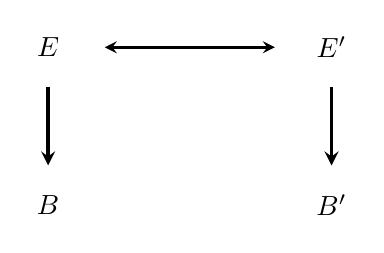
\begin{tikzpicture}[x=12mm,y=10mm,>=stealth]
\node (EL) at (0,0) {$E$};\node (ER) at (3,0) {$E'$};
\node (BL) at (0,-2) {$B$};\node (BR) at (3,-2) {$B'$};
\draw[<->,line width=0.9pt] (0.6,0) -- (2.4,0);
\draw[->,line width=1.2pt] (0,-0.5) -- (0,-1.5);
\draw[->,line width=1.2pt] (3,-0.5) -- (3,-1.5);
\end{tikzpicture}
\end{center}

\Unclear{GELFAND-P000098}{sheaf-isomorphism-diagram}{Верхний ряд $E\leftrightarrow E^{\prime}$, две толстые стрелки вниз к $B$, $B^{\prime}$. Верхние концы и наконечники густые; их точное очертание не установлено. Между $B$ и $B^{\prime}$ горизонтальной стрелки не видно.}
\end{GelfandAdjacentEvidence}
\begin{GelfandAdjacentEvidence}{GELFAND-P000098}{11}


Если $E$ — подпучок ф-ий, то
$B\longrightarrow B^{\prime}$ индуцирует $E^{\prime}\longrightarrow E$.

\SourceFigure{GELFAND-P000098}{contravariance}{В строке $B\longrightarrow B^{\prime}$ индуцирует $E^{\prime}\longrightarrow E$; штрихи у вторых букв подняты вверх.}
\end{GelfandAdjacentEvidence}
\begin{GelfandAdjacentEvidence}{GELFAND-P000098}{12}


(A priori только коммут.) Треб., чтобы изом.
был изом., возникн. из сообр. базы. (естеств.!)
просто совпадение!

\SourceFigure{GELFAND-P000098}{base-isomorphism}{«(A priori только коммут.) Треб., чтобы изом. был изом., возникн. из сообр. базы. (естеств.!) просто совпадение!»}
\end{GelfandAdjacentEvidence}
\begin{GelfandAdjacentEvidence}{GELFAND-P000098}{13}


$C^2\setminus0$ это
\begin{tikzpicture}[baseline=(w.base),x=1mm,y=1mm]
\node[inner sep=0pt] (w) at (0,0) {предалг.};
\draw[line width=0.4pt] (-11,4) -- (-3,4);
\draw[line width=0.4pt] (3,6) -- (13,6);
\node[inner sep=0pt] at (-1,4) {$\cdot$};
\end{tikzpicture}
мн-зие.

\Unclear{GELFAND-P000098}{punctured-prevariety}{$C^2\setminus0$ это предалг. мн-зие. Над предалг. две разнесённые горизонтальные черты, правая выше; возле нижней точка. Их роль и привязка к словам не установлены. Написано $C$, без дополнительной вертикальной черты.}
\end{GelfandAdjacentEvidence}
\begin{GelfandAdjacentEvidence}{GELFAND-P000098}{14}


Выбр. $2$ прямые[?].

\Unclear{GELFAND-P000098}{two-lines-word}{После «Выбр. 2» тесное «прямые»[?] / «прямки»[?]; средние и конечные штрихи густые.}
\end{GelfandAdjacentEvidence}
\begin{GelfandAdjacentEvidence}{GELFAND-P000098}{15}


$1$-е на $x\ne0$, $2$-е $y\ne0$.
Наше мн-во — их объедин. Каждое из
них афф. мн-зие.

\SourceFigure{GELFAND-P000098}{two-open-cover}{«$1$-е на $x\ne0$, $2$-е $y\ne0$». Наше мн-во — их объедин.; каждое из них афф. мн-зие.}
\end{GelfandAdjacentEvidence}
\begin{GelfandAdjacentEvidence}{GELFAND-P000098}{16}


\begin{center}
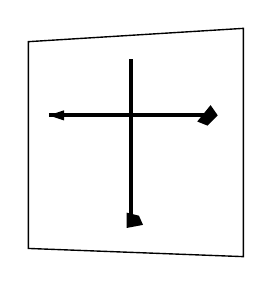
\begin{tikzpicture}[x=13mm,y=13mm]
\draw[line width=0.5pt] (0,0) -- (2.1,-0.08) -- (2.1,2.15) -- (0,2.02) -- cycle;
\draw[line width=1.5pt] (1,0.25) -- (1,1.85);
\draw[line width=1.5pt] (0.2,1.3) -- (1.8,1.3);
\path[fill=black] (0.2,1.3) -- (0.35,1.35) -- (0.35,1.25) -- cycle;
\path[fill=black] (1.65,1.24) -- (1.78,1.4) -- (1.85,1.3) -- (1.75,1.2) -- cycle;
\path[fill=black] (0.96,0.35) -- (1.08,0.32) -- (1.12,0.23) -- (0.96,0.2) -- cycle;
\end{tikzpicture}
\end{center}

\Unclear{GELFAND-P000098}{punctured-plane-diagram}{В прямоугольной рамке пересекаются толстые вертикальная и горизонтальная линии. Левый конец заострён, правый и нижний утолщены; роль утолщений и точная форма возможных наконечников не установлены. Буквенных подписей и отдельного кружка в пересечении не видно.}
\end{GelfandAdjacentEvidence}
\begin{GelfandAdjacentEvidence}{GELFAND-P000098}{17}


Затем сог\underline{лас.} пу\underline{чки} колец уже ясно[?].

\Unclear{GELFAND-P000098}{sheaf-agreement}{«Затем соглас. пучки колец уже ясно»[?]; конечное слово ясно[?] / легко[?]. Ниже строки две раздельные черты — под концом «соглас.» и под частью «пучки»; точная привязка подчёркивания остаётся неуверенной.}
\end{GelfandAdjacentEvidence}
\begin{GelfandAdjacentEvidence}{GELFAND-P000098}{18}


Точки $\overset{\text{пред}}{\vee}$ алг. мн-зий могут быть неразделимы для ф-ий.

\SourceFigure{GELFAND-P000098}{inseparable-points}{Над промежутком перед «алг.» вписано «пред» с V-образным знаком вставки. «Точки» написано густо; окончание следующей строки «ф-ий».}
\end{GelfandAdjacentEvidence}
\begin{GelfandAdjacentEvidence}{GELFAND-P000098}{19}


\uwave{Пример пр. афф. $\overset{\underbrace{\text{пред-}}}{\text{алг.}}$ мн-зий.}

\SourceFigure{GELFAND-P000098}{example-heading}{Заголовок «Пример пр. афф. алг. мн-зий.» подчёркнут волнистой линией. Над «алг.» вставлено «пред-» с нижней фигурной скобкой. Сокращение «пр.» не раскрыто.}
\end{GelfandAdjacentEvidence}
\begin{GelfandAdjacentEvidence}{GELFAND-P000098}{20}


\begin{equation*}\begin{gathered}
p_1(x_1,\ldots,x_n\text{[?]})=0,\\[-2pt]
\mathord{,}\quad-\qquad-\ \text{[?]}\\[-2pt]
p_k(x_1,\ldots,x_n\text{[?]})=0,\\
Q(x_1,\ldots,x_n\text{[?]})\ne0.
\end{gathered}\end{equation*}

\Unclear{GELFAND-P000098}{last-coordinate-indices}{В трёх строках последние индексы $x_n$[?] / $x_m$[?] густые; во второй строке есть добавленный верхний штрих. Нижний индекс $1$ при первом $p$ с густым горизонтальным основанием. Между первой и второй строками три отдельные короткие отметки: левая запятой-/точкой-подобная и две черты; их роль не установлена.}
\end{GelfandAdjacentEvidence}
\begin{GelfandAdjacentEvidence}{GELFAND-P000098}{21}


Последнее усл. не обязательно, любое [зачёркнутое слово неразборчиво]
афф. алг. мн. можно задать, не используя этих
[зачёркнутое слово неразборчиво] условиях
($\exists$ мн., ему изоморфное).

\Unclear{GELFAND-P000098}{affine-condition-cancels}{После «любое» густо отменено слово с длинными горизонтальными штрихами и петлёй слева; ниже после «этих» второе густо зачёркнутое слово. Уверенное буквенное чтение обоих не установлено.}

\SourceFigure{GELFAND-P000098}{final-affine-condition}{«Последнее усл. не обязательно»; далее «не используя этих … условиях»; ниже «($\exists$ мн., ему изоморфное)». Окончание «условиях» сохранено.}
\end{GelfandAdjacentEvidence}





\begin{GelfandAdjacentEvidence}{GELFAND-P000099}{1}
\SourcePage{GELFAND-P000099}{66}

Берём $(x,y)$ с условием

\begin{equation*}\begin{cases}P_i(x)=0,\\Q(x)y-1=0\end{cases}\end{equation*}

\hfill $(x_1,\ldots,x_n,y)$

\SourceFigure{GELFAND-P000099}{opening-graph}{Система с левой фигурной скобкой: $P_i(x)=0$, $Q(x)y-1=0$. Справа вверху $(x_1,\ldots,x_n,y)$; номер $66$ с угловой чертой слева и снизу.}
\end{GelfandAdjacentEvidence}
\begin{GelfandAdjacentEvidence}{GELFAND-P000099}{2}


Они изоморфны.

\SourceFigure{GELFAND-P000099}{isomorphic}{«Они изоморфны.»}
\end{GelfandAdjacentEvidence}
\begin{GelfandAdjacentEvidence}{GELFAND-P000099}{3}


Пусть есть кол.[?] $P(x)$ и идеал $I\text{[?]}$ — первое афф. алг. мн.
$P(y)$ $J$ — $2$-е афф. алг. мн.

Их произведение —
— кольцо $P(x,y)$ с идеалом

\begin{equation*}\left\{I\text{[?]}\otimes[P(y)]\mathbin{+\!\text{[?]}}[P(x)]\otimes J\right\}\end{equation*}

\Unclear{GELFAND-P000099}{product-ideal-notation}{Первый идеал $I$[?] / $J$[?]: верхняя черта и нижний левый загиб, в формуле нижняя петля. Между слагаемыми густо переписанный $+$[?] / $\oplus$[?]. Сокращение перед первым кольцом кол.[?] / коль.[?].}

\SourceFigure{GELFAND-P000099}{product-intro}{«Их произведение —» и следующая строка «— кольцо $P(x,y)$ с идеалом»: две отдельные черты тире.}
\end{GelfandAdjacentEvidence}
\begin{GelfandAdjacentEvidence}{GELFAND-P000099}{4}


\hfill{\fontencoding{OT1}\fontfamily{cmr}\selectfont\textcircled{?}}\,[?]

\Unclear{GELFAND-P000099}{tensor-circled-symbol}{Справа обведён ?-/2-подобный знак; под изогнутым основным штрихом отдельная нижняя точка. Чтение не установлено.}
\end{GelfandAdjacentEvidence}
\begin{GelfandAdjacentEvidence}{GELFAND-P000099}{5}


(как мн-во — обычн. произв.)

\SourceFigure{GELFAND-P000099}{product-set}{«(как мн-во — обычн. произв.)».}
\end{GelfandAdjacentEvidence}
\begin{GelfandAdjacentEvidence}{GELFAND-P000099}{6}


Кольцо ф-ий на нём — тенз. пр. колец ф-ий на тех мн.

\SourceFigure{GELFAND-P000099}{function-ring}{«Кольцо ф-ий на нём — тенз. пр. колец ф-ий на тех мн.».}
\end{GelfandAdjacentEvidence}
\begin{GelfandAdjacentEvidence}{GELFAND-P000099}{7}


Пр. произв. любых предалг. мн. — [зачёркнутая запись неразборчива]

\begin{center}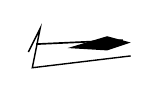
\begin{tikzpicture}[x=1mm,y=1mm]
\draw[line width=0.5pt] (0,2) -- (1.5,5) -- (0.5,0) -- (13,1.5);
\draw[line width=0.6pt] (1,3) -- (12,3.5);
\path[fill=black] (5,2.5) -- (10,4) -- (13,3.2) -- (10,2.2) -- cycle;
\end{tikzpicture}\end{center}

\SourceFigure{GELFAND-P000099}{product-heading}{«Пр. произв. любых предалг. мн. —». Сокращение «Пр.» оставлено.}
\end{GelfandAdjacentEvidence}
\begin{GelfandAdjacentEvidence}{GELFAND-P000099}{8}


$X,Y$ — $\overset{\text{пред}}{\vee}$алг. многообр.

\SourceFigure{GELFAND-P000099}{prevariety-insertion}{Над промежутком перед алг. вписано пред, снизу V-образный знак вставки; в строке $X,Y$.}
\end{GelfandAdjacentEvidence}
\begin{GelfandAdjacentEvidence}{GELFAND-P000099}{9}


$\{U_i\}$ $\{V_j\}$ — $2$ покр. афф. откр. подмногообр.
$X\times Y$ покрыто $U_i\times V_j$. Это есть напр.[?] мн-обр.

\Unclear{GELFAND-P000099}{affine-covers}{Верхняя строка $\{U_i\}$, $\{V_j\}$ — $2$ покр. афф. откр. подмногообр.; ниже $X\times Y$ покрыто $U_i\times V_j$. После «Это есть» напр.[?]-подобное сокращение, неуверенно прочитанное.}
\end{GelfandAdjacentEvidence}
\begin{GelfandAdjacentEvidence}{GELFAND-P000099}{10}


[Густо зачёркнутая начальная запись неразборчива] Заметим, что произв. мн. не есть произв.
топ. пр-в (топ. не есть топ. произв.).

\Unclear{GELFAND-P000099}{product-and-heading-cancels}{После тире в строке о произведении густая отмена; ниже отдельная угловая черта и чёрная помета. Перед «Заметим» густо зачёркнута начальная запись. Буквенное чтение отмен не установлено.}

\SourceFigure{GELFAND-P000099}{product-topology}{«Заметим, что произв. мн. не есть произв. топ. пр-в (топ. не есть топ. произв.)».}
\end{GelfandAdjacentEvidence}
\begin{GelfandAdjacentEvidence}{GELFAND-P000099}{11}



Рассм. $X\times X$. Выберем в нём\par
\hspace*{12mm}{\small в нём структ.}

\SourceFigure{GELFAND-P000099}{structure-line}{В строке «Рассм. $X\times X$. Выберем в нём»; под строкой отдельно «в нём структ.».}
\end{GelfandAdjacentEvidence}
\begin{GelfandAdjacentEvidence}{GELFAND-P000099}{12}


Предалг.[?] подмногообр. — замкнутое подмн-во в тп.[?] Зарисского.
Оно само предалг. мн-зие.

\Unclear{GELFAND-P000099}{subvariety-prefix-correction}{В начале «Предалг.»[?], средние буквы густо переписаны; прежние штрихи не прочитаны.}

\Unclear{GELFAND-P000099}{subvariety-definition}{«подмногообр. — замкнутое подмн-во в тп.[?] Зарисского». Сокращение тп.[?] / топ.[?] тесное. Следующая строка «Оно само предалг. мн-зие».}
\end{GelfandAdjacentEvidence}
\begin{GelfandAdjacentEvidence}{GELFAND-P000099}{13}


В $X\times X$ есть диагональ $(x,x)$. Если она
замкнута, то мн-зие наз. алгебраическим.

\SourceFigure{GELFAND-P000099}{diagonal-variety}{«В $X\times X$ есть диагональ $(x,x)$. Если она замкнута, то мн-зие наз. алгебраическим».}
\end{GelfandAdjacentEvidence}
\begin{GelfandAdjacentEvidence}{GELFAND-P000099}{14}


[Это станд. — предпучок наз. пучком, если диагональ
замкнута.



Топ. в $X$ отделимая, если диаг. $X\times X$
замкнута.)
\Unclear{GELFAND-P000099}{presheaf-diagonal-term}{«предпучок наз. пучком, если диагональ замкнута». Написание первого слова предпучок; тесные соединённые штрихи сохранены в оригинале рядом.}

\Unclear{GELFAND-P000099}{separation-topology}{«Топ. в $X$ отделимая, если диаг. $X\times X$ замкнута.)»; начало отступления квадратной скобкой, конец круглой. Привязка несимметричных скобок не установлена.}
\end{GelfandAdjacentEvidence}
\begin{GelfandAdjacentEvidence}{GELFAND-P000099}{15}


\underline{Пример} предалг., но не алг. $X$.
$(U_1,U_2)$ — покр., $U_1,U_2$ — изом. прямой.
$U_1\cap U_2$ изом. прямой с выкол. точкой.

\SourceFigure{GELFAND-P000099}{double-origin-example}{Пример подчёркнуто прямой линией; $(U_1,U_2)$, $U_1,U_2$, $U_1\cap U_2$ и выкол. точка.}
\end{GelfandAdjacentEvidence}
\begin{GelfandAdjacentEvidence}{GELFAND-P000099}{16}



\begin{center}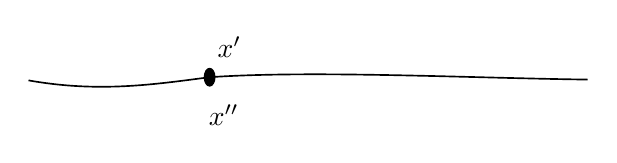
\begin{tikzpicture}[x=10mm,y=10mm]
\draw[line width=0.6pt] (0,0) .. controls (0.9,-0.16) and (1.6,-0.05) .. (2.3,0.04) .. controls (3.6,0.13) and (5.6,0.03) .. (7.1,0.01);
\path[fill=black] (2.3,0.04) ellipse[x radius=0.075,y radius=0.12];
\node at (2.55,0.42) {$x'$};\node at (2.48,-0.44) {$x''$};
\end{tikzpicture}\end{center}

\Unclear{GELFAND-P000099}{double-origin-diagram}{Одна почти горизонтальная линия с утолщённой точкой; над ней $x^{\prime}$, под ней $x^{\prime\prime}$. Точная форма утолщения не установлена.}
\end{GelfandAdjacentEvidence}
\begin{GelfandAdjacentEvidence}{GELFAND-P000099}{17}



\begin{tikzpicture}[baseline=0mm,x=1mm,y=1mm]
\path[fill=black] (0,0.6) -- (0.7,2.6) -- (5,2.6) -- (3.2,1.5) -- (6.6,1.5) -- (5.7,0) -- (1,0) -- cycle;
\draw[line width=0.7pt] (0,0.6) -- (0,-1);
\end{tikzpicture}\quad Проверить, что диаг. не замкнута.

\Unclear{GELFAND-P000099}{final-instruction}{Перед «Проверить» отдельный густой чёрный знак с двумя правыми выступами; его роль и точное очертание не установлены. «Проверить, что диаг. не замкнута».}
\end{GelfandAdjacentEvidence}





\begin{GelfandAdjacentEvidence}{GELFAND-P000100}{1}
\SourcePage{GELFAND-P000100}{unlabelled}

\underline{Классы циклов по модулю лин. экв.}

\SourceFigure{GELFAND-P000100}{cycle-heading}{Весь заголовок «Классы циклов по модулю лин. экв.» подчёркнут прямой линией.}
\end{GelfandAdjacentEvidence}
\begin{GelfandAdjacentEvidence}{GELFAND-P000100}{2}


[более точный инв., чем когом.)

\Unclear{GELFAND-P000100}{heading-aside}{«более точный инв., чем когом.»; начальная скобка угловатая, с нижней правой полкой, чтение [ / ( не вполне установлено; закрывающая скобка круглая.}
\end{GelfandAdjacentEvidence}
\begin{GelfandAdjacentEvidence}{GELFAND-P000100}{3}


$X$ — алг. многообр., подмн. — замкн. мн-во в топ. Зарисского.

\SourceFigure{GELFAND-P000100}{variety-definition}{$X$ — алг. многообр.; «подмн. — замкн. мн-во в топ. Зарисского».}
\end{GelfandAdjacentEvidence}
\begin{GelfandAdjacentEvidence}{GELFAND-P000100}{4}


$V_i$ — подмногообр.

\SourceFigure{GELFAND-P000100}{subvariety-label}{$V_i$ — подмногообр.; нижний индекс $i$.}
\end{GelfandAdjacentEvidence}
\begin{GelfandAdjacentEvidence}{GELFAND-P000100}{5}



\begin{equation*}\sum\underset{\text{фор.[?]}}{a_iV_i}\text{ — циклы}\qquad(a_i\text{ — целые})\end{equation*}

\Unclear{GELFAND-P000100}{formal-cycle}{Под слагаемым суммы краткая запись фор.[?] / форм.[?]; после отчётливых ф, о и р тесный верхний выходной штрих. Формула $\sum a_iV_i$ и справа $(a_i\text{ — целые})$.}
\end{GelfandAdjacentEvidence}
\begin{GelfandAdjacentEvidence}{GELFAND-P000100}{6}


$\sum b_iU_i$. $2$ цикла линейно экв., если



$X\times P^1$\qquad в нём есть подмн.\quad $\begin{gathered}X\times a,\\X\times b\\a,b\in P^1\end{gathered}$
\SourceFigure{GELFAND-P000100}{second-cycle}{$\sum b_iU_i$. «$2$ цикла линейно экв., если»; точка после $U_i$.}

\SourceFigure{GELFAND-P000100}{fiber-subvarieties}{$X\times P^1$; слова «в нём есть подмн.»; справа $X\times a$, ниже $X\times b$ и $a,b\in P^1$.}
\end{GelfandAdjacentEvidence}
\begin{GelfandAdjacentEvidence}{GELFAND-P000100}{7}


($P^1$ покр. двумя об. прям. — алг. мн.)

\SourceFigure{GELFAND-P000100}{projective-cover}{«($P^1$ покр. двумя об. прям. — алг. мн.)»; сокращение об. и обе скобки.}
\end{GelfandAdjacentEvidence}
\begin{GelfandAdjacentEvidence}{GELFAND-P000100}{8}




\begin{tikzpicture}[baseline=0mm,x=1mm,y=1mm]
\path[fill=black] (0,0) -- (-0.5,2.1) -- (-0.9,3.6) -- (0.2,3.2) -- (0.4,4.6) -- (1.1,3.5) -- (1.8,4.3) -- (2,2.1) -- (2.6,1.7) -- (1.6,1.4) -- (1.7,0) -- (0.9,0.5) -- cycle;
\end{tikzpicture}\quad Они кан. изом. $X$.

\Unclear{GELFAND-P000100}{margin-star}{Слева чёрная вертикальная звёздочко-/буквоподобная помета с выступами. Воспроизведена приближённая форма; буквенное чтение и назначение не установлены.}

\SourceFigure{GELFAND-P000100}{canonical-isomorphism}{«Они кан. изом. $X$.»}
\end{GelfandAdjacentEvidence}
\begin{GelfandAdjacentEvidence}{GELFAND-P000100}{9}


$2$ цикла экв., если [зачёркнуто: неразборчиво] $\exists$ $3$-й цикл, $W\text{[?]}\in X\times P^1$,
дающий в пересеч. с [зачёркнуто: неразборчиво] $X\times a$ первый, а
с $X\times b$ второй.

\Unclear{GELFAND-P000100}{cycle-equivalence-cancels}{После «если» отменено выражение с начальным в-подобным штрихом; после «с» отменено ещё одно слово с нижней петлёй. Полное чтение отмен не установлено.}

\Unclear{GELFAND-P000100}{cycle-equivalence-body}{«$\exists$ $3$-й цикл, $W\text{[?]}\in X\times P^1$»; буква $W$[?] имеет тесные восходящие штрихи, возможен N-подобный облик. За цикл короткая нижняя запятая. Продолжение с $X\times a$ и $X\times b$ в трёх строках.}
\end{GelfandAdjacentEvidence}
\begin{GelfandAdjacentEvidence}{GELFAND-P000100}{10}


\underline{Пример.} $X$ — поверхность, $U,V$ — кривые.

\SourceFigure{GELFAND-P000100}{example-heading}{Пример. подчёркнуто вместе с точкой; $X$ — поверхность, $U,V$ — кривые.}
\end{GelfandAdjacentEvidence}
\begin{GelfandAdjacentEvidence}{GELFAND-P000100}{11}


Они лин. экв., если $\exists$ [зачёркнутый знак неразборчив] ф-я с нулями
на $U$ и полюсами на $V$.

\Unclear{GELFAND-P000100}{rational-function-cancel}{Между знаком существования и ф-я густой маленький знак: замкнутая горизонтальная петля с поперечным штрихом; буквенное чтение не установлено.}

\SourceFigure{GELFAND-P000100}{linear-equivalence}{«Они лин. экв., если $\exists$ … ф-я с нулями на $U$ и полюсами на $V$.»}
\end{GelfandAdjacentEvidence}
\begin{GelfandAdjacentEvidence}{GELFAND-P000100}{12}


Рассм. $X\times P^1$. Берём в нём $a=0$ и $b\mathrel{=\!\text{[?]}}\infty$.
В $X\times P^1$ берём цикл $(x,f(x))$

\Unclear{GELFAND-P000100}{graph-example}{Перед $\infty$ после $b$ густая короткая горизонтальная запись, $=$[?]; обе отдельные черты не отделяются уверенно. В следующей строке $(x,f(x))$: высокий штрих $f$ с поперечной чертой. Начальное Рассм. с густыми нижними штрихами, отдельное подчёркивание не установлено.}
\end{GelfandAdjacentEvidence}
\begin{GelfandAdjacentEvidence}{GELFAND-P000100}{13}


\underline{Опред. классов Черна[?]} (алг. мн-зий)

\Unclear{GELFAND-P000100}{chern-name-overwrite}{В текущем слове Черна[?] густо переписаны внутренние и конечные штрихи; прежние буквы не отделены.}

\SourceFigure{GELFAND-P000100}{chern-heading}{Прямая черта проходит под Опред. классов и именем Черна; справа «(алг. мн-зий)».}
\end{GelfandAdjacentEvidence}
\begin{GelfandAdjacentEvidence}{GELFAND-P000100}{14}


Они зад. с кон.[?] аксиом.

\Unclear{GELFAND-P000100}{axiom-abbreviation}{Перед аксиом. краткое кон.[?] / нек.[?]; тесные средние соединения не позволяют установить порядок букв.}

\SourceFigure{GELFAND-P000100}{axiom-phrase}{«Они зад. с … аксиом.»; точка в конце строки.}
\end{GelfandAdjacentEvidence}
\begin{GelfandAdjacentEvidence}{GELFAND-P000100}{15}


[Зачёркнутый начальный знак неразборчив] Функтор из категории [зачёркнутый обведённый знак неразборчив]

\Unclear{GELFAND-P000100}{category-cancellations}{Слева перед Функтор густо отменён прежний знак с высоким левым штрихом; после категории отменён и обведён петлёй ещё один знак. Буквенные чтения не установлены.}

\SourceFigure{GELFAND-P000100}{functor-line}{«Функтор из категории»; справа и слева отдельные отмены.}
\end{GelfandAdjacentEvidence}
\begin{GelfandAdjacentEvidence}{GELFAND-P000100}{16}


Алгебр. пучок, алгебр. $K$-функтор.

\SourceFigure{GELFAND-P000100}{k-functor}{«Алгебр. пучок, алгебр. $K$-функтор.»}
\end{GelfandAdjacentEvidence}
\begin{GelfandAdjacentEvidence}{GELFAND-P000100}{17}


\hfill\begin{minipage}{0.52\linewidth}$A(X)$ —\\— гр. лин. экв.\\\hspace*{18mm}циклов\end{minipage}

\SourceFigure{GELFAND-P000100}{cycle-group}{Справа $A(X)$ —; на следующей строке ещё одно тире перед гр. лин. экв., ниже циклов.}
\end{GelfandAdjacentEvidence}
\begin{GelfandAdjacentEvidence}{GELFAND-P000100}{18}


Отобр. $K(X)\longrightarrow A(X)$ линейное.

\SourceFigure{GELFAND-P000100}{linear-map}{«Отобр. $K(X)\longrightarrow A(X)$ линейное.»; направленная вправо стрелка.}
\end{GelfandAdjacentEvidence}
\begin{GelfandAdjacentEvidence}{GELFAND-P000100}{19}


\underline{Аксиомы.}

\SourceFigure{GELFAND-P000100}{axiom-heading}{Аксиомы. подчёркнуто прямой линией.}
\end{GelfandAdjacentEvidence}
\begin{GelfandAdjacentEvidence}{GELFAND-P000100}{20}


1. [Зачёркнутое продолжение неразборчиво]

\Unclear{GELFAND-P000100}{first-axiom-cancel}{Последняя запись: 1. и густо зачёркнутая строка с двумя длинными поперечными штрихами. Под ней до нижнего края новых читаемых аксиом нет.}
\end{GelfandAdjacentEvidence}




\begin{GelfandAdjacentEvidence}{GELFAND-P000101}{1}

\SourcePage{GELFAND-P000101}{67}
$18/\overline{\underline X}$. \underline{И.М. Гельфанд.}
\par\hspace*{4mm}$X$

$E_1,\ldots,E_n$
\begin{equation*}
\Gamma(E_1)\overset d\longrightarrow\Gamma(E_2)
\overset d\longrightarrow\cdots\overset d\longrightarrow\Gamma(E_n)
\end{equation*}
[Справа зачёркнуто: Дифф.[?] опер.[?]] Элл. комплекс.
\Unclear{GELFAND-P000101}{top-cancellations}{Две густо зачёркнутые записи: Дифф.[?] / Диффер.[?] и опер.[?]. Отчётливые остатки не устанавливают всех отменённых букв.}
\end{GelfandAdjacentEvidence}
\begin{GelfandAdjacentEvidence}{GELFAND-P000101}{2}

\begin{equation*}
d\bigl(f^m(x)s(x)\bigr)\big|_{x_0}=\sigma(d,\eta)s(x_0),
\qquad df\big|_{x_0}=\eta
\end{equation*}
$\sigma$ — символ дифф. опер.
\begin{equation*}
0\longrightarrow E_{1,x_0}\underset{\sigma(d,\eta)}\longrightarrow E_{2,x_0}
\longrightarrow\cdots\overset{\sigma(d,\eta)}\longrightarrow E_{n,x_0}\longrightarrow0.
\end{equation*}
\SourceFigure{GELFAND-P000101}{symbol-sequence-placement}{У первой стрелки между слоями $\sigma(d,\eta)$ внизу, у последней — сверху; нули на обоих концах.}
\end{GelfandAdjacentEvidence}
\begin{GelfandAdjacentEvidence}{GELFAND-P000101}{3}

\underline{Отобр.} $T:\Gamma(E)\longrightarrow\Gamma(E)$.
\hfill$\Gamma(E_i)\longrightarrow\Gamma(E_i)$

$f:X\longrightarrow X$

$\varphi$ индуц.[?] рассл.
\Unclear{GELFAND-P000101}{bundle-contraction}{Между $\varphi$ и рассл. связная запись индуц.[?] / эндом.[?]; первая буква густо переписана, в середине высокий штрих с верхней дужкой.}
\end{GelfandAdjacentEvidence}
\begin{GelfandAdjacentEvidence}{GELFAND-P000101}{4}


\begin{center}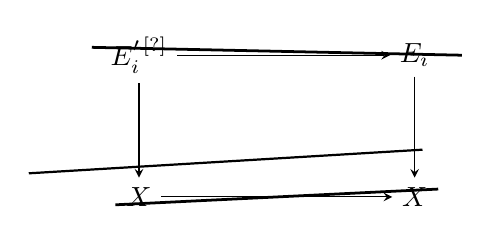
\begin{tikzpicture}[x=1mm,y=1mm,>=stealth]
\node(a)at(0,18){$E_i^{\prime\,[?]}$};\node(b)at(35,18){$E_i$};
\node(c)at(0,0){$X$};\node(e)at(35,0){$X$};
\draw[->](a)--(b);\draw[->](a)--(c);\draw[->](b)--(e);\draw[->](c)--(e);
\draw[line width=1pt](-6,19)--(41,18);
\draw[line width=.8pt](-14,3)--(36,6);
\draw[line width=1pt](-3,-1)--(38,1);
\end{tikzpicture}\end{center}

\Unclear{GELFAND-P000101}{cancelled-bundle-square}{Зачёркнутый квадрат: верхние $E_i$, слева возможен добавленный верхний штрих; стрелки вправо и вниз, внизу $X\to X$. Несколько длинных отменяющих черт; точные скрытые индексы и очертания не установлены.}
\end{GelfandAdjacentEvidence}
\begin{GelfandAdjacentEvidence}{GELFAND-P000101}{5}


\begin{center}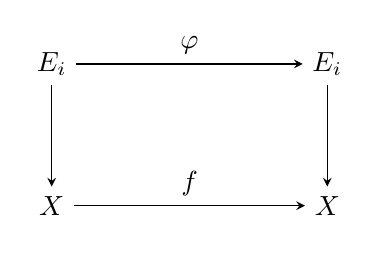
\begin{tikzpicture}[x=1mm,y=1mm,>=stealth]
\node(a)at(0,18){$E_i$};\node(b)at(35,18){$E_i$};
\node(c)at(0,0){$X$};\node(e)at(35,0){$X$};
\draw[->](a)--node[above]{$\varphi$}(b);\draw[->](a)--(c);
\draw[->](b)--(e);\draw[->](c)--node[above]{$f$}(e);
\end{tikzpicture}\end{center}

\SourceFigure{GELFAND-P000101}{active-bundle-square}{Верхняя стрелка $E_i\overset\varphi\longrightarrow E_i$, две стрелки вниз; нижняя $X\overset f\longrightarrow X$.}
\end{GelfandAdjacentEvidence}
\begin{GelfandAdjacentEvidence}{GELFAND-P000101}{6}

(В простейш. случаях $\varphi$ определяет $f$ —
— формы $f$ опред. отобр. кас. векторов)

Эндом., если коммут. с $d$.

$T$ есть опер. в $C^\infty$-пр-ве. Теорема свод. к изуч. следа
(он счит. $2$-мя способами)

\underline{Теорема 1.} Комплекс имеет конечные
[зачёркнутое слово неразборчиво] гомологии.
\Unclear{GELFAND-P000101}{theorem-cancel}{Между конечные и гомологии густо зачёркнуто слово; видны верхняя дужка и нижний штрих. Полное чтение не установлено.}
\end{GelfandAdjacentEvidence}
\begin{GelfandAdjacentEvidence}{GELFAND-P000101}{7}


Пусть $\omega^n$ — форма пор. $n$ на $X$, не обращ. в $0$.
Введём с её помощью эрмитову структуру. (Пусть она
сущ. раз и навсегда. \underline{Неинв}ариантно, но проще.)
\begin{equation*}
\int\langle s,\alpha(s')\rangle=\int_X\overline{(s,s')}\,\omega.
\end{equation*}
\SourceFigure{GELFAND-P000101}{hermitian-pairing}{Слева угловые скобки, $s,\alpha(s')$; справа интеграл по $X$, черта над $(s,s')$, затем $\omega$.}
\end{GelfandAdjacentEvidence}
\begin{GelfandAdjacentEvidence}{GELFAND-P000101}{8}

\begin{equation*}d^*\underset{\mathrm{def}}{=}\alpha^{-1}\cdot d'\circ\alpha.\end{equation*}
\Unclear{GELFAND-P000101}{adjoint-definition}{Верхняя часть начального $d$ густая; рядом звёздочка. Под равенством def; справа $\alpha^{-1}\cdot d'\circ\alpha$. Отдельного уверенно читаемого знака в густой части нет.}
\end{GelfandAdjacentEvidence}
\begin{GelfandAdjacentEvidence}{GELFAND-P000101}{9}

$s\in\Gamma(E)$, $s'\in\Gamma_c(E')$.
\Unclear{GELFAND-P000101}{dual-section-index}{В первом $\Gamma$ нижняя часть переписана; при втором $\Gamma$ нижняя открытая петля, читается $c$, возможен о-подобный облик.}
\end{GelfandAdjacentEvidence}
\begin{GelfandAdjacentEvidence}{GELFAND-P000101}{10}


$E'$ — сопр. пучок.
\begin{equation*}\Box\underset{\mathrm{def}}{=}d^*d+dd^*\end{equation*}
[Отдельная чёрная помета слева внизу от определения.]
\Unclear{GELFAND-P000101}{middle-ink-mark}{Отдельное густое пятно с мелкими точками и косыми штрихами; буквенное чтение и назначение не установлены.}
\end{GelfandAdjacentEvidence}
\begin{GelfandAdjacentEvidence}{GELFAND-P000101}{11}

($d'$ — просто сопр. оператор)

$\Box$ — эллипт. оператор, перев. каждое $\Gamma(E_i)$ в себя.

$\Gamma_\lambda(E)$ — сечения, удовл. ур-ю $\Box s=\lambda s$.
Т.к. $\Box$ эллиптичен, то $\forall\lambda$ кон. число разл. лин. незав. соб. ф-й
[густой отдельный знак неразборчив].
\Unclear{GELFAND-P000101}{eigenfunction-end-sign}{После ф-й отдельная густая замкнутая чёрная запись с внутренними вертикальными штрихами; H-подобное чтение не установлено.}
\end{GelfandAdjacentEvidence}
\begin{GelfandAdjacentEvidence}{GELFAND-P000101}{12}

\begin{equation*}\Box d=d\Box\end{equation*}
\begin{equation*}
\Gamma_\lambda(E_1)\overset d\longrightarrow\Gamma_\lambda(E_2)
\overset d\longrightarrow\cdots\longrightarrow\Gamma_\lambda(E_n)
\end{equation*}
\SourceFigure{GELFAND-P000101}{lower-sequence-punctuation}{У второй круглой скобки низкий выходной штрих, соприкасающийся со следующей строкой; отдельная запятая не установлена.}
\end{GelfandAdjacentEvidence}
\begin{GelfandAdjacentEvidence}{GELFAND-P000101}{13}

Введём группы гомологий
[ниже зачёркнутая формула неразборчива].
\Unclear{GELFAND-P000101}{homology-cancel}{Ниже группы гомологий два длинных поперечных штриха через короткую формулу; видны вертикальные основания и верхний косой штрих. Полное чтение не установлено.}
\end{GelfandAdjacentEvidence}
\begin{GelfandAdjacentEvidence}{GELFAND-P000101}{14}


\begin{center}\begin{tikzpicture}[x=1mm,y=1mm]
\node[anchor=west](h)at(0,7){$H^i(\Gamma_\lambda(E))=\operatorname{Ker}d\big|_{\Gamma_{\lambda\text{[?]}}(E_i)}$};
\draw[line width=.6pt](110,-9)--(127,12);
\node[anchor=west](den)at(115,-8){$\operatorname{Im}d\text{[?]}$};
\draw[line width=.8pt](115,-8)--(132,-7);
\node[anchor=west]at(136,-8){$\ldots$};
\end{tikzpicture}\end{center}

\Unclear{GELFAND-P000101}{kernel-restriction}{После вертикальной черты $\Gamma$ с густым нижним знаком $\lambda$[?], затем $(E_i)$; начальное Ker с прописной K.}
\end{GelfandAdjacentEvidence}
\begin{GelfandAdjacentEvidence}{GELFAND-P000101}{15}

\Unclear{GELFAND-P000101}{homology-denominator}{Справа наклонная дробная черта; внизу густо зачёркнутое $\operatorname{Im}d$[?], затем три раздельные точки. Чтение отменённых средних штрихов не установлено.}
\end{GelfandAdjacentEvidence}
\begin{GelfandAdjacentEvidence}{GELFAND-P000102}{16}



\SourcePage{GELFAND-P000102}{unlabelled}
Без док-ва в этой работе утв. теорема Ходжа
\begin{equation*}
H^i(\Gamma_\lambda(E))^{*\text{[?]}}=
\begin{cases}H^i(E)&\lambda=0\\0&\lambda\ne0.\end{cases}
\end{equation*}
\Unclear{GELFAND-P000102}{complex-star}{Над правыми закрывающими скобками маленькая густая звёздочкообразная помета; точная привязка к скобкам и обозначению не установлена.}
\end{GelfandAdjacentEvidence}
\begin{GelfandAdjacentEvidence}{GELFAND-P000102}{17}

\uwave{Дынин.} При $\lambda\ne0$ — здесь $0$.
($d$ при $\lambda\ne0$ перев. соб. ф-и
[зачёркнутое слово неразборчиво] точн. компл.
\Unclear{GELFAND-P000102}{dynin-cancel}{Перед точн. компл. густо зачёркнута короткая запись. После неё точн. компл.; последние буквы тесные, над ними отдельная дужка. Буквенное чтение отмены не установлено.}
\end{GelfandAdjacentEvidence}
\begin{GelfandAdjacentEvidence}{GELFAND-P000102}{18}


\begin{center}\begin{tikzpicture}
\node[inner sep=2mm](k){$H^i(\Gamma_\lambda(E))=\operatorname{Ker}(\Box-\lambda)$};
\draw[line width=.5pt]([xshift=-2mm,yshift=1mm]k.south west)
 --([xshift=-2mm,yshift=-2mm]k.south west)
 --([xshift=2mm,yshift=-2mm]k.south east)
 --([xshift=2mm,yshift=1mm]k.south east);
\end{tikzpicture}\end{center}

это теор. Ходжа $\forall\lambda$
\SourceFigure{GELFAND-P000102}{dynin-kernel-claim}{Под формулой и по обоим краям три стороны рамки, сверху открыто. Справа $\operatorname{Ker}(\Box-\lambda)$, начальная K прописная.}
\end{GelfandAdjacentEvidence}
\begin{GelfandAdjacentEvidence}{GELFAND-P000102}{19}

($\forall$ элл. опер. $\underset{?}{\text{[зачёркнуто: неразборчиво]}}$
$\Box-\lambda$ — новая буква, снова теор. Ходжа\ldots
\Unclear{GELFAND-P000102}{dynin-general-cancel}{После элл. опер. густо отменено короткое сокращение; непосредственно под ним вопросительный знак. Полное чтение не установлено.}
\end{GelfandAdjacentEvidence}
\begin{GelfandAdjacentEvidence}{GELFAND-P000102}{20}

\SourceFigure{GELFAND-P000102}{dynin-parentheses}{Видны открывающие круглые скобки перед $d$ и перед $\forall$ элл. опер.; в последней строке после Ходжа три раздельные точки. Закрывающие скобки в этом фрагменте не прочитаны.}
\end{GelfandAdjacentEvidence}
\begin{GelfandAdjacentEvidence}{GELFAND-P000102}{21}


\uwave{Бернштейн.} То же. $H^i(\Gamma_\lambda(E))=0$, $\lambda\ne0$.
Пусть $s\in\Gamma_\lambda(E_i)$ и пусть $ds=0$.
[?] $\Box s=dd^*s$. Тогда $\lambda s=d(d^*s)$
и $s=d\left(\frac{d^*s}{\lambda}\right)$,
$d^*s$ есть соб. ф-я ($d^*$ коммут. с $\Box$).
\Unclear{GELFAND-P000102}{bernstein-square-prefix}{Перед $\Box$ высокий густой штрих с замкнутой верхней петлёй и нижним косым выходом: $d$[?] / открывающая скобка[?]. Чтение не установлено.}
\end{GelfandAdjacentEvidence}
\begin{GelfandAdjacentEvidence}{GELFAND-P000102}{22}

\SourceFigure{GELFAND-P000102}{bernstein-division}{Запись $s=d\left(\frac{d^*s}{\lambda}\right)$: длинная горизонтальная черта проходит вблизи основания внешнего $d$ и через скобки; справа отдельная запятая.}
\end{GelfandAdjacentEvidence}
\begin{GelfandAdjacentEvidence}{GELFAND-P000102}{23}


$d^*s\in C^\infty$ след. из \underline{теор.} об \underline{элл.} ур-ях.
\underline{Опять Гельфанд.}
При $\lambda=0$ букв. перен. док-во Ходжа.
\SourceFigure{GELFAND-P000102}{source-emphasis}{Под Дынин. и Бернштейн. волнистые линии; под Опять Гельфанд. прямая линия. В строке перед последним заголовком отдельно подчёркнуты теор. и элл.}
\end{GelfandAdjacentEvidence}
\begin{GelfandAdjacentEvidence}{GELFAND-P000102}{24}

\begin{equation*}\Gamma(E)=\sum\Gamma_\lambda(E)\qquad(\text{дискр. спектр})\end{equation*}
\SourceFigure{GELFAND-P000102}{spectral-decomposition}{$\Gamma(E)=\sum\Gamma_\lambda(E)$; под знаком суммы отдельного индекса не видно.}
\end{GelfandAdjacentEvidence}
\begin{GelfandAdjacentEvidence}{GELFAND-P000102}{25}

Кроме опер. $T$ введём
\begin{equation*}\fbox{$T_\lambda=\pi_\lambda\circ T\circ i_\lambda,$}\end{equation*}
где $i_\lambda:\Gamma_\lambda(E)\longrightarrow\Gamma(E)$,
$\pi_\lambda:\Gamma(E)\longrightarrow\Gamma_\lambda(E)$ — проекция ортог.
\SourceFigure{GELFAND-P000102}{projected-operator}{Прямоугольная рамка вокруг $T_\lambda=\pi_\lambda\circ T\circ i_\lambda$; в конце внутри рамки запятая. Ниже строка с $\pi_\lambda$ и проекция ортог.; над рамкой (дискр. спектр).}
\end{GelfandAdjacentEvidence}
\begin{GelfandAdjacentEvidence}{GELFAND-P000102}{26}


(опер. $T$ в этой клетке) Число Лефшица для $T$.

$T$ — отобр. сечений, тем самым отобр. сечений $\Gamma(E)\to\Gamma(E)$
\begin{equation*}L(T,E)=\sum(-1)^i\operatorname{tr}(T_i^*|H_i\text{[?]}).\end{equation*}
\Unclear{GELFAND-P000102}{lefschetz-space}{После вертикальной черты густо переписана H-подобная буква; отдельный $i$ внизу справа, выше него точка. Чтение основной буквы и положения индекса остаётся неуверенным: $H_i$[?] / $H^i$[?].}
\end{GelfandAdjacentEvidence}
\begin{GelfandAdjacentEvidence}{GELFAND-P000102}{27}

В силу теор. Ходжа $T_{\lambda=0}=T^*$.
\hfill$\Pi_0\text{[?]}=T^{*\text{[?]}}$
\Unclear{GELFAND-P000102}{hodge-stars}{Слева $T_{\lambda=0}=T^*$. Справа первая буква с длинной верхней чертой и нижним $0$: $\Pi_0$[?] / $\pi_0$[?] / $T_0$[?]. Над правым $T$ густая звёздочкообразная запись; одна или две наложенные звёздочки не различены уверенно.}
\end{GelfandAdjacentEvidence}
\begin{GelfandAdjacentEvidence}{GELFAND-P000102}{28}

\begin{gather*}
\sum(-1)^i\operatorname{tr}(T_0|E_i)=L(T,E)\\
\sum(-1)^i\operatorname{tr}(T_\lambda|E_i)=0\qquad\lambda\ne0
\end{gather*}
[Справа две густо зачёркнутые записи неразборчивы.]
\Unclear{GELFAND-P000102}{right-cancellations}{В правом поле две маленькие густые отмены: верхняя с нижней петлёй, нижняя с длинным восходящим косым штрихом. Буквенное чтение не установлено.}
\end{GelfandAdjacentEvidence}
\begin{GelfandAdjacentEvidence}{GELFAND-P000102}{29}


(след в гом. всё равно, что след в самих пр-вах)

(По теор. Ходжа $H^i(E)=\Gamma_0(E_i)$)
\begin{equation*}\Box s=0\Longrightarrow\underline{ds=0}.\end{equation*}
\SourceFigure{GELFAND-P000102}{zero-hodge-implication}{В $\Box s=0\Longrightarrow ds=0$ толстая переписанная стрелка; под $ds=0$ горизонтальная черта, справа отдельная точка.}
\end{GelfandAdjacentEvidence}
\begin{GelfandAdjacentEvidence}{GELFAND-P000102}{30}

(из непоср.[?] опр. и т.п.)
\Unclear{GELFAND-P000102}{positive-aside}{После из густая связная запись непоср.[?] / полож.[?]; справа опр. и т.п., затем закрывающая круглая скобка. Над первыми средними штрихами густая правка.}
\end{GelfandAdjacentEvidence}
\begin{GelfandAdjacentEvidence}{GELFAND-P000102}{31}


Надо придать смысл $\sum(-1)^i\operatorname{tr}(T|E_i)$. Его регуляриз.
\par $2$-мя способами.
\SourceFigure{GELFAND-P000102}{regularization-order}{В первой строке Надо придать смысл, сумма и справа Его регуляриз. Ниже слева $2$-мя способами.}
\end{GelfandAdjacentEvidence}
\begin{GelfandAdjacentEvidence}{GELFAND-P000103}{32}



\SourcePage{GELFAND-P000103}{68}
В конеч. $\Gamma_\lambda(E)$
\begin{equation*}d:\Gamma_\lambda(E_1)\longrightarrow\Gamma_\lambda(E_2)\longrightarrow\cdots\end{equation*}
(конечномерность)
$T$ — его отобр. в себя. Тогда
\begin{equation*}\sum(-1)^i\operatorname{tr}T|_{E_i}=\sum(-1)^i\operatorname{tr}T|_{H_i}\end{equation*}
(а $H^i=0$)
\par(инвар. эйлер. характеристики)
\SourceFigure{GELFAND-P000103}{finite-trace-complex}{В первой цепочке две стрелки, затем многоточие; в скобках конечномерность. В равенстве следов после вертикальных черт $E_i$ и $H_i$ с нижними индексами; в следующей скобке $H^i=0$ с верхним $i$.}
\end{GelfandAdjacentEvidence}
\begin{GelfandAdjacentEvidence}{GELFAND-P000103}{33}


Рассм.
\begin{equation*}\sum_\lambda(1+\lambda)^{-z}\operatorname{tr}(T_\lambda|E_i)=\operatorname{tr}^{z}(E_i)\end{equation*}
\underline{Теорема.} Ряд сх. при $\operatorname{Re}z>\frac12\dim X$
(об асимпт. соб. ф-й) (Данфорд и Шварц, т.2)
\par Это анал. ф-я $z$ в полупл.
\SourceFigure{GELFAND-P000103}{regularized-trace}{У $(1+\lambda)$ показатель $-z$, с отдельной короткой чертой минуса. Справа $\operatorname{tr}^{z}(E_i)$. Ниже подчёркнуто Теорема.; $\operatorname{Re}z>\frac12\dim X$ и две скобки.}
\end{GelfandAdjacentEvidence}
\begin{GelfandAdjacentEvidence}{GELFAND-P000103}{34}

\begin{equation*}L(T,E)=\sum(-1)^i\operatorname{tr}^{z}E_i\qquad\forall z\end{equation*}
\SourceFigure{GELFAND-P000103}{all-z-identity}{В левой части $L(T,E)$; справа у следа верхний $z$, затем $E_i$ без скобок. Правее отдельное $\forall z$ с густым первым знаком.}
\end{GelfandAdjacentEvidence}
\begin{GelfandAdjacentEvidence}{GELFAND-P000103}{35}

(всё, кроме сходимости, доказано [густо переписанный знак неразборчив]

—
\begin{center}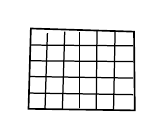
\begin{tikzpicture}[x=1cm,y=1cm]
\draw[line width=.6pt](0,0)--(1.35,-.02)--(1.34,.98)--(.03,1.02)--cycle;
\draw[line width=.45pt](.21,.01)--(.24,.96);
\draw[line width=.45pt](.43,-.01)--(.46,.98);
\draw[line width=.45pt](.65,.01)--(.65,.98);
\draw[line width=.45pt](.86,-.01)--(.87,.99);
\draw[line width=.45pt](1.08,-.01)--(1.10,.99);
\draw[line width=.45pt](.02,.20)--(1.33,.18);
\draw[line width=.45pt](.01,.41)--(1.33,.39);
\draw[line width=.45pt](.02,.61)--(1.33,.60);
\draw[line width=.45pt](.02,.81)--(1.33,.80);
\end{tikzpicture}\end{center}
)
\Unclear{GELFAND-P000103}{proof-overwrite}{После доказано густая вертикальная запись с нижним косым петлеобразным выходом. Отдельные прежние буквы не разделены даже при увеличении; точное чтение не установлено.}
\end{GelfandAdjacentEvidence}
\begin{GelfandAdjacentEvidence}{GELFAND-P000103}{36}

\SourceFigure{GELFAND-P000103}{proof-grid}{После тире маленькая прямоугольная сетка с горизонтальными и вертикальными штрихами. Наборное воссоздание показывает видимые линии; густые пересечения и края не вполне различимы. Буквенной подписи и определённой роли у сетки не прочитано.}
\end{GelfandAdjacentEvidence}
\begin{GelfandAdjacentEvidence}{GELFAND-P000103}{37}



Т.к. $T\sim$ ограничен (асимпт. соб. ф-й)
\par(при аналит. прод. при $z=0$ полюс)
\SourceFigure{GELFAND-P000103}{bounded-tilde}{После T отдельный волнистый знак $\sim$, затем ограничен; в скобках асимпт. соб. ф-й. Ниже отдельная скобка при аналит. прод. при $z=0$ полюс.}
\end{GelfandAdjacentEvidence}
\begin{GelfandAdjacentEvidence}{GELFAND-P000103}{38}


\underline{Пример.} $S^1$
\begin{center}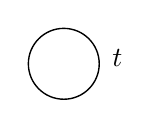
\begin{tikzpicture}[x=1cm,y=1cm]
\draw[line width=.5pt](0,0)circle(.45);
\node at(.68,.08){$t$};
\end{tikzpicture}\end{center}
$d=\frac d{dt}$, элл. опер., $\Box=\frac{d^2}{dt^2}$.
\SourceFigure{GELFAND-P000103}{circle-derivative}{Окружность с $t$ справа. В знаменателе первой производной начальный $d$ густо переписан, затем $t$; прежние штрихи не разделены. У $\Box$ записано $d^2/dt^2$ с положительным знаком.}
\end{GelfandAdjacentEvidence}
\begin{GelfandAdjacentEvidence}{GELFAND-P000103}{39}


$T=(f,\varphi)$,
\begin{gather*}dS(x)=s(x)\\Ts(x)=\varphi(x)s(f(x))\end{gather*}
\SourceFigure{GELFAND-P000103}{section-equations}{Слева $T=(f,\varphi)$ и запятая. Справа сверху $dS(x)=s(x)$: первая S прописная, вторая s строчная. Ниже $Ts(x)=\varphi(x)s(f(x))$.}
\end{GelfandAdjacentEvidence}
\begin{GelfandAdjacentEvidence}{GELFAND-P000103}{40}

\begin{center}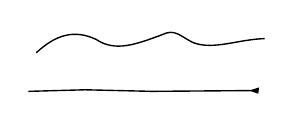
\begin{tikzpicture}[x=1cm,y=1cm]
\draw[line width=.5pt](0,.55)..controls(.25,.78)and(.48,.85)..(.76,.72)
 ..controls(1,.56)and(1.25,.65)..(1.60,.78)
 ..controls(1.76,.86)and(1.83,.76)..(1.99,.68)
 ..controls(2.25,.58)and(2.56,.72)..(2.90,.73);
\draw[line width=.5pt](-.10,.06)--(.62,.08)--(1.47,.06)--(2.72,.07);
\path[fill=black](2.70,.07)--(2.83,.11)--(2.82,.03)--cycle;
\end{tikzpicture}\end{center}
\SourceFigure{GELFAND-P000103}{small-wave}{Слева под $T=(f,\varphi)$ отдельная волнистая линия; ниже почти горизонтальный штрих с утолщённым правым концом. Наборное воссоздание сохраняет общий ход линий; направление утолщения и назначение рисунка не установлены. Подписей осей и функций нет.}
\end{GelfandAdjacentEvidence}
\begin{GelfandAdjacentEvidence}{GELFAND-P000103}{41}


\underline{Определение} [?] псевдодифф. опер:
\Unclear{GELFAND-P000103}{definition-prefix}{Между заголовком и псевдодифф. густой переписанный знак с правой вертикалью и несколькими поперечными штрихами: P[?] / неразборчиво. Надёжное буквенное чтение не установлено.}
\end{GelfandAdjacentEvidence}
\begin{GelfandAdjacentEvidence}{GELFAND-P000103}{42}

$X$ — многообр. $\Gamma(E)$, $\Gamma(F)$ — 2 рассл. на $X$
\begin{equation*}P:\Gamma_c(E)\longrightarrow\Gamma(F)\end{equation*}
$\Gamma_c(E)$ — сеч. с комп. носителем.
[Зачёркнуто: Наз.[?]]
\Unclear{GELFAND-P000103}{pseudo-cancel}{Перед Лин. опер. наз. короткое сокращение с длинным нижним косым штрихом отмены. Наз.[?]; прежние буквы густо соединены и не прочитаны уверенно. После него отдельная точка.}
\end{GelfandAdjacentEvidence}
\begin{GelfandAdjacentEvidence}{GELFAND-P000103}{43}

Лин. опер. наз. псевдодифф., если $\exists$ послед. чисел
$n_1>n_2>n_3>\cdots\to-\infty$

и уд. след. условиям
\begin{equation*}e^{-i\lambda g}\underline{P}(e^{i\lambda g}s)\end{equation*}
$g\in\Gamma(1)$ ($C^\infty$-ф-я),
1 — трив. пучок, $s(x)\in\Gamma_c(E)$, $dg\ne0$ на $\operatorname{supp}s$,
если есть асимпт. разлож.




\SourcePage{GELFAND-P000104}{unlabelled}
\begin{equation*}\sim\sum_0^\infty P_j(s,g)\lambda^{n_j}\end{equation*}
\Unclear{GELFAND-P000103}{order-signs}{Три знака с остриями вправо. У первого и третьего густые нижние концы и отдельные мелкие следы; средний переписан и сливается со следующим n. Отдельные нижние черты равенства не установлены: $>$[?] / $\geq$[?].}
\end{GelfandAdjacentEvidence}
\begin{GelfandAdjacentEvidence}{GELFAND-P000103}{44}

\SourceFigure{GELFAND-P000103}{pseudo-definition}{Заголовок Определение подчёркнут прямой линией. В формуле с экспонентами у P короткая нижняя черта; показатели $-i\lambda g$ и $i\lambda g$. В скобках $C^\infty$-ф-я. Справа $dg\ne0$, ниже на $\operatorname{supp}s$ и запятая.}
\end{GelfandAdjacentEvidence}
\begin{GelfandAdjacentEvidence}{GELFAND-P000103}{45}

\Unclear{GELFAND-P000103}{bottom-mark}{Справа от асимпт. разлож. короткая густая отдельная помета: верхняя петля, горизонтальный выход вправо и нижний выступ. Буквенное чтение и привязка не установлены.}
\end{GelfandAdjacentEvidence}
\begin{GelfandAdjacentEvidence}{GELFAND-P000104}{46}


\SourceFigure{GELFAND-P000104}{asymptotic-continuation}{Продолжение формулы: отдельный $\sim$, нижний предел $0$ без $j=$, верхний $\infty$, затем $P_j(s,g)\lambda^{n_j}$.}
\end{GelfandAdjacentEvidence}
\begin{GelfandAdjacentEvidence}{GELFAND-P000104}{47}


$26/\underline{\overline{X}}$ \underline{Продолжение.} Элл. комплекс.
\SourceFigure{GELFAND-P000104}{continuation-header}{У X в дате отдельные верхняя и нижняя черты. Продолжение. подчёркнуто отдельно; далее Элл. комплекс.}
\end{GelfandAdjacentEvidence}
\begin{GelfandAdjacentEvidence}{GELFAND-P000104}{48}

В $E_i$ — эрмитова метрика и в $X$ — интегрирование.
Вв. опер. $d^*$, $\Box=dd^*+d^*d$, $\Box d=d\Box$
\par $\Box s=\lambda s$, $\Box$ самосопр. и полож., эллиптичен, $\lambda>0$.
$\Box s=0\Longrightarrow ds=0$
\begin{equation*}d\Gamma_\lambda(E_i)\subset\Gamma_\lambda(E_{i+1})\end{equation*}
\Unclear{GELFAND-P000104}{laplacian-commutation-edge}{Справа в $\Box d=d\Box$ правый край последнего квадрата прерывистый и бледный. Остальные стороны различимы; точная правая граница знака в имеющемся скане повреждена. Ниже отдельно записано $\lambda>0$ и $\Box s=0\Longrightarrow ds=0$.}
\end{GelfandAdjacentEvidence}
\begin{GelfandAdjacentEvidence}{GELFAND-P000104}{49}


\begin{equation*}0\overset{d}{\longrightarrow}\Gamma(E)\overset{d}{\longrightarrow}\Gamma(F)\overset{d}{\longrightarrow}0\end{equation*}
$d$ — просто эллипт. оператор, $ds=0$ — ядро.
Образ $s_1=ds_*$,
\Unclear{GELFAND-P000104}{image-preimage}{У первого s нижний знак похож на $1$, возможен $i$. Знак после второго s звездообразный, расположен близко к строке; его высота неоднозначна: $s_1=ds_*$ / $s_i=ds^*$ / неразборчивый индекс.}
\end{GelfandAdjacentEvidence}
\begin{GelfandAdjacentEvidence}{GELFAND-P000104}{50}

\uwave{Гомологии:} $\operatorname{Ker}d|_E$, $\operatorname{Coker}d|_F$.
Число Лефшица — \underline{индекс}
\SourceFigure{GELFAND-P000104}{two-term-homology}{У всех трёх стрелок первой цепочки надписано d. Гомологии: подчёркнуто волнистой линией; Ker и Coker начинаются прописными буквами. У индекс отдельная прямая нижняя черта.}
\end{GelfandAdjacentEvidence}
\begin{GelfandAdjacentEvidence}{GELFAND-P000104}{51}


\begin{equation*}\Gamma_\lambda(E_i)\overset{d}{\longrightarrow}\Gamma_\lambda(E_{i+1})\longrightarrow\cdots\end{equation*}
уже конечномерн. комплекс,
его гом. $=0$ при $\lambda\ne0$ и $=H^i$
[зачёркнуто: при] [неразборчивая фраза]
при $\lambda=0$.
\Unclear{GELFAND-P000104}{zero-cohomology-words}{После $H^i$ густо зачёркнуто при. Затем соединённые петли: самое конеч.[?] / само конеч.[?]; точное чтение первого слова не установлено. В конце при $\lambda=0$.}
\end{GelfandAdjacentEvidence}
\begin{GelfandAdjacentEvidence}{GELFAND-P000104}{52}


$T_i^*\quad H^i$
\begin{equation*}\sum(-1)^i\operatorname{tr}(T_i^*)=L(T,E)\end{equation*}
Вычислить через неподв. точки.
\par $T$ — отобр. $X$, коммут. с $d$.
\SourceFigure{GELFAND-P000104}{lefschetz-actions}{Слева отдельные $T_i^*$ и $H^i$, без стрелки между ними. Справа равенство с $L(T,E)$. Ниже T — отобр. X, коммут. с d.; справа Вычислить через неподв. точки.}
\end{GelfandAdjacentEvidence}
\begin{GelfandAdjacentEvidence}{GELFAND-P000104}{53}


$T$ есть отобр. $\Gamma_\lambda(E_i)$
Введ. операторы $\pi_\lambda$ и $i_\lambda$.
влож. $\Gamma_\lambda$ во всё $\Gamma$ и проектир. на
[зачёркнуто: неразборчивая запись]

$\Gamma_\lambda(E_i)$.
\Unclear{GELFAND-P000104}{projection-cancel}{После на короткая густо зачёркнутая запись с верхней петлёй и поперечными штрихами. Прежние буквы не разделены; далее отдельное действующее $\Gamma_\lambda(E_i)$.}
\end{GelfandAdjacentEvidence}
\begin{GelfandAdjacentEvidence}{GELFAND-P000104}{54}


\begin{equation*}T_\lambda=\pi_\lambda\cdot T i_\lambda\end{equation*}
(выдел. клетки, соотв. $\Gamma_\lambda$)
\SourceFigure{GELFAND-P000104}{projection-definition}{Записаны вложение $\Gamma_\lambda$ во всё $\Gamma$ и проектирование на $\Gamma_\lambda(E_i)$. В формуле одна точка умножения перед T; между T и $i_\lambda$ отдельной точки нет. Ниже скобка о выделении клеток.}
\end{GelfandAdjacentEvidence}
\begin{GelfandAdjacentEvidence}{GELFAND-P000104}{55}


Коммут. ненужно, дост.
[густой переписанный знак]

\begin{center}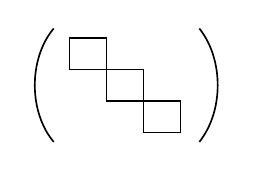
\begin{tikzpicture}[x=1cm,y=1cm]
\draw[line width=.6pt](0,0)--(.47,0)--(.47,-.40)--(0,-.40)--cycle;
\draw[line width=.6pt](.47,-.40)--(.94,-.40)--(.94,-.80)--(.47,-.80)--cycle;
\draw[line width=.6pt](.94,-.80)--(1.41,-.80)--(1.41,-1.20)--(.94,-1.20)--cycle;
\draw[line width=.6pt](-.20,.12)..controls(-.52,-.26)and(-.52,-.94)..(-.20,-1.32);
\draw[line width=.6pt](1.65,.12)..controls(1.96,-.27)and(1.96,-.93)..(1.65,-1.32);
\end{tikzpicture}\end{center}
в клетках.
\Unclear{GELFAND-P000104}{cell-cancel}{Между дост. и рисунком густая вертикальная запись с двумя тёмными скоплениями и косым нижним выходом. Буквенное чтение не установлено; знак сохранён отдельно от клеток.}
\end{GelfandAdjacentEvidence}
\begin{GelfandAdjacentEvidence}{GELFAND-P000104}{56}


\SourceFigure{GELFAND-P000104}{diagonal-cells}{Три пустых квадрата идут сверху слева вниз вправо внутри круглых скобок; соседние углы касаются. Наборное воссоздание сохраняет три контура и скобки; точные размеры и густые стыки не установлены.}
\end{GelfandAdjacentEvidence}
\begin{GelfandAdjacentEvidence}{GELFAND-P000104}{57}


Тогда \fbox{$T^*=T_0$}
\begin{equation*}0\longrightarrow\Gamma_0(E_1)\overset{d}{\longrightarrow}\Gamma_0(E_2)\overset{d}{\longrightarrow}\cdots\end{equation*}
все $d=0$ т.к. $\Box s=0$.
\SourceFigure{GELFAND-P000104}{zero-complex-frame}{Равенство $T^*=T_0$ заключено в полную прямоугольную рамку. У первой стрелки из 0 надписи нет, над двумя следующими d; затем многоточие. Справа все $d=0$, ниже т.к. $\Box s=0$.}
\end{GelfandAdjacentEvidence}
\begin{GelfandAdjacentEvidence}{GELFAND-P000104}{58}


Все гомологии в $\Gamma_0$
\begin{center}\begin{tikzpicture}[x=1cm,y=1cm]
\node[anchor=west]at(0,0){$\Gamma(E_i)=\Gamma_0(E_i)+$};
\node at(4.65,0){$\Gamma_{\lambda_1}(E_i)$};
\node at(6.00,0){$+$};\node at(6.80,0){$\cdots$};
\draw[line width=.6pt,->](4.65,-.32)--(4.65,-.92);
\draw[line width=.6pt](6.80,-.30)--(6.78,-.92);
\node at(5.75,-1.20){гомол. $0$};
\end{tikzpicture}\end{center}
\SourceFigure{GELFAND-P000104}{decomposition-arrows}{Под $\Gamma_{\lambda_1}(E_i)$ короткая стрелка вниз; под многоточием отдельный вертикальный штрих с густым нижним концом. Ниже гомол. 0. Под $\Gamma_0(E_i)$ стрелки нет. У правого штриха отдельное остриё не установлено.}
\end{GelfandAdjacentEvidence}
\begin{GelfandAdjacentEvidence}{GELFAND-P000104}{59}


В 1-й строчке
[зачёркнуто: неразборчивое слово]

ядра $\Gamma_0(E_i)$
\Unclear{GELFAND-P000104}{first-row-cancel}{Перед ядра короткая горизонтальная зачёркнутая запись с густыми соединёнными штрихами. Надёжного буквенного чтения нет.}
\end{GelfandAdjacentEvidence}
\begin{GelfandAdjacentEvidence}{GELFAND-P000104}{60}


\begin{center}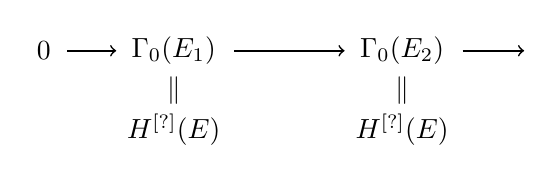
\begin{tikzpicture}[x=1cm,y=1cm]
\node at(0,0){$0$};\node at(1.65,0){$\Gamma_0(E_1)$};\node at(4.55,0){$\Gamma_0(E_2)$};
\draw[line width=.6pt,->](.30,0)--(.92,0);
\draw[line width=.6pt,->](2.42,0)--(3.82,0);
\draw[line width=.6pt,->](5.32,0)--(6.10,0);
\node at(1.65,-.50){$\Vert$};\node at(4.55,-.50){$\Vert$};
\node at(1.65,-1.00){$H^{[?]}(E)$};\node at(4.55,-1.00){$H^{[?]}(E)$};
\end{tikzpicture}\end{center}
\Unclear{GELFAND-P000104}{cohomology-overwrite}{Под двумя членами цепочки вертикальные двойные штрихи и записи $H^{[?]}(E)$. Оба верхних знака густо переписаны: $H^*(E)$ / $H^i(E)$ / неразборчивая степень. Прежние штрихи даже при увеличении не разделены. Последняя стрелка цепочки не имеет видимого продолжения или многоточия.}
\end{GelfandAdjacentEvidence}
\begin{GelfandAdjacentEvidence}{GELFAND-P000104}{61}

\underline{Замеч.} $\pi_\lambda$ коммутирует с $d$.
\SourceFigure{GELFAND-P000104}{commuting-projection-remark}{Замеч. подчёркнуто прямой линией; далее $\pi_\lambda$ коммутирует с d.}
\end{GelfandAdjacentEvidence}
\begin{GelfandAdjacentEvidence}{GELFAND-P000104}{62}

\begin{equation*}\left\{\begin{aligned}\sum(-1)^i\operatorname{tr}(T_0^i)&=L(T,E)\\(-1)^i\operatorname{tr}(T_\lambda^i)&=0\end{aligned}\right.\end{equation*}
\Unclear{GELFAND-P000104}{last-sum-absent}{Общая левая фигурная скобка. Только первая строка начинается со $\sum$; перед $(-1)^i$ во второй строке отдельной суммы не видно. У T в обеих строках верхний i; нижние знаки 0 и $\lambda$.}
\end{GelfandAdjacentEvidence}
\begin{GelfandAdjacentEvidence}{GELFAND-P000105}{63}



\SourcePage{GELFAND-P000105}{69}
Если есть послед. пр-в
\begin{equation*}0\longrightarrow A_1\overset{d}{\longrightarrow}A_2\overset{d}{\longrightarrow}\cdots\overset{d}{\longrightarrow}A_n\longrightarrow0,\qquad d^2=0.\end{equation*}
и отобр. $T_i$, комм. с $d$. Тогда
\begin{equation*}\underset{\text{в цепях}}{\sum(-1)^i\operatorname{tr}T_i}=\underset{\text{в гомол.}}{\sum(-1)^i\operatorname{tr}(T_i^*)}\qquad(\text{ф-ла Эйлера})\end{equation*}
(ф-ла Эйлера получ., если взять $T=E$)
\SourceFigure{GELFAND-P000105}{euler-chain-annotations}{В первой цепочке крайние стрелки без надписей, внутренние с d. Под левой суммой отдельный штрих и в цепях; под правой штрих и в гомол. Справа скобка ф-ла Эйлера.}
\end{GelfandAdjacentEvidence}
\begin{GelfandAdjacentEvidence}{GELFAND-P000105}{64}


\underline{Док-во}: предст.
\begin{equation*}A_i=\underset{\text{$Z$ 3-х слаг.}}{Z}+C_Z,\qquad Z=B+\text{доп.}\end{equation*}
и потом рассм. $T$ там.
\SourceFigure{GELFAND-P000105}{proof-decomposition}{Док-во подчёркнуто прямой линией; двоеточие справа от черты. Под первым Z отдельная запись Z 3-х слаг. Во второй записи $Z=B+\text{доп.}$; далее и потом рассм. T там.}
\end{GelfandAdjacentEvidence}
\begin{GelfandAdjacentEvidence}{GELFAND-P000105}{65}

$\operatorname{tr}T_\lambda$ дост. заменить на $\operatorname{tr}T_\lambda^*$,
а [зачёркнуто: неразборчивая запись] $H_\lambda=0$.
\Unclear{GELFAND-P000105}{homology-cancel}{Перед $H_\lambda=0$ длинная густо зачёркнутая запись с петлями по обоим концам и горизонтальным штрихом. Прежние буквы не разделены.}
\end{GelfandAdjacentEvidence}
\begin{GelfandAdjacentEvidence}{GELFAND-P000105}{66}


Введём
\begin{equation*}\operatorname{tr}^z(E_i)=\sum_\lambda(1+\lambda)^{-z}\operatorname{tr}(T_\lambda^*|E_i)\end{equation*}
при $\operatorname{Re}z>\frac12\dim X$,
\SourceFigure{GELFAND-P000105}{regularized-trace-definition}{У суммы нижний $\lambda$, у множителя показатель $-z$, у $T_\lambda$ верхняя звёздочка. Следующая строка при $\operatorname{Re}z>\frac12\dim X$ и запятая.}
\end{GelfandAdjacentEvidence}
\begin{GelfandAdjacentEvidence}{GELFAND-P000105}{67}

[Справа:]
\begin{equation*}\lambda_n\sim n^{K/\dim X}\end{equation*}
\Unclear{GELFAND-P000105}{eigenvalue-power}{В числителе показателя K-подобный знак с прямым левым штрихом и двумя правыми ветвями: $K$ / $\kappa$.}
\end{GelfandAdjacentEvidence}
\begin{GelfandAdjacentEvidence}{GELFAND-P000105}{68}

\begin{equation*}\sum(-1)^i\operatorname{tr}^z(T_i^i)=L(T,E)\qquad\text{при всех }z.\end{equation*}
\Unclear{GELFAND-P000105}{trace-argument}{После tr в скобках густой T с нижним i-подобным знаком и отдельным верхним i-подобным знаком: $T_i^i$ / $T_i$ / неразборчивый верхний знак.}
\end{GelfandAdjacentEvidence}
\begin{GelfandAdjacentEvidence}{GELFAND-P000105}{69}


\uwave{Теорема о продолжении}
(ссылка на Narashimhan a[?] и др.)
\Unclear{GELFAND-P000105}{continuation-name}{Латинское имя с соединёнными m/h/n-подобными петлями и отдельным конечным a: Narashimhan a[?] / Narasimhcan a / Narasimhana. Ниже Nirenberg, с густо переписанным окончанием; далее ещё два имени.}
\end{GelfandAdjacentEvidence}
\begin{GelfandAdjacentEvidence}{GELFAND-P000105}{70}

[Над и др.: катасэ.[?]]
\Unclear{GELFAND-P000105}{continuation-side-name}{Отдельная маленькая запись над и др.: катаcэ. / катасэ. / неразборчиво. Последний знак похож на э; часть начертаний допускает латинское c.}
\end{GelfandAdjacentEvidence}
\begin{GelfandAdjacentEvidence}{GELFAND-P000105}{71}

[Ниже: Nirenberg, Cohna[?], Hörmander.]
\Unclear{GELFAND-P000105}{continuation-middle-name}{Среднее латинское имя между запятыми: Cohna / Cohn a. Между h и конечным a соединённые густые штрихи; точное разделение букв не установлено.}
\end{GelfandAdjacentEvidence}
\begin{GelfandAdjacentEvidence}{GELFAND-P000105}{72}

\par $\operatorname{tr}^zT^i$ продолжима во всю плоскость, аналитична во всей плоскости (!) и при $z=0$

\begin{equation*}\operatorname{tr}^0(T^i)=\operatorname{tr}^{[?]}(T^i)\end{equation*}

где $\operatorname{tr}^b$ — след, счит. обычн. способом через обобщ. ф-и.
\SourceFigure{GELFAND-P000105}{continuation-theorem-heading}{Заголовок Теорема о продолжении подчёркнут волнистой линией. В тексте дважды во всю/всей плоскость/плоскости, отдельная скобка (!) и при $z=0$. У T верхний i.}
\end{GelfandAdjacentEvidence}
\begin{GelfandAdjacentEvidence}{GELFAND-P000105}{73}

\Unclear{GELFAND-P000105}{trace-superscript-overwrite}{Верхний знак у второго tr густо переписан и сливается с окружающими штрихами: b[?] / неразборчиво. Ниже и слева в дальнейшем ясно записано $\operatorname{tr}^b$.}
\end{GelfandAdjacentEvidence}
\begin{GelfandAdjacentEvidence}{GELFAND-P000105}{74}



$T=E$ не годится (получ. $\zeta(s)$[?] с полюсами), но рассм.
[Вставка под $T=E$:] $(\operatorname{tr}E=\infty\text{ при }z=0)$.

опер. [неразборчивый знак], им. конечн. число неподв. точек (простых).
\Unclear{GELFAND-P000105}{identity-pole-insertion}{Перед (s) крупный зигзагообразный знак с нижним закруглённым выходом: $\zeta$[?] / $\Sigma$[?]. Под строкой отдельная скобка $\operatorname{tr}E=\infty$ при $z=0$.}
\end{GelfandAdjacentEvidence}
\begin{GelfandAdjacentEvidence}{GELFAND-P000105}{75}


\Unclear{GELFAND-P000105}{operator-mark}{После опер. густая вертикальная переписанная запись с несколькими поперечными выступами и нижними ножками; надёжного буквенного чтения нет. Далее запятая, им. конечн. число неподв. точек (простых).}
\end{GelfandAdjacentEvidence}
\begin{GelfandAdjacentEvidence}{GELFAND-P000105}{76}


$\operatorname{tr}^b$: $T$ имеется в виде ядра, $\int\kappa(x,x)\,dx$.
\Unclear{GELFAND-P000105}{kernel-letter-shape}{Буква ядра K-/к-подобная: $\kappa$ / $K$. В интеграле короткий плотный знак, в формуле двух аргументов более высокий левый штрих. По рукописной высоте алфавит и регистр не установлены.}
\end{GelfandAdjacentEvidence}
\begin{GelfandAdjacentEvidence}{GELFAND-P000105}{77}

$\operatorname{tr}^b$ — счит. через неподв. точки.
[Над неподв.: (обобщ. ф-и).]
(Вариант послед. ф-й, сход.[?] к $\delta$-ф-и)
Некоторый вар. b-следа.
\Unclear{GELFAND-P000105}{distribution-approximation-overwrite}{В скобке слово перед к $\delta$-ф-и густо переписано: сход.[?] / неразборчивое начало. Прежние штрихи не разделены. Над предыдущим неподв. отдельная вставка (обобщ. ф-и).}
\end{GelfandAdjacentEvidence}
\begin{GelfandAdjacentEvidence}{GELFAND-P000105}{78}

[Справа:] $\delta(x,a)$ — $\delta$ в точке $a$.
\begin{equation*}s(x)\longrightarrow\varphi s(f(x))\end{equation*}
(пробр. следов) $x\longrightarrow f(x)$
\begin{equation*}\kappa(x,y)=\delta(y\,{[?]}\,f(x))\end{equation*}
\Unclear{GELFAND-P000105}{kernel-argument}{Первый аргумент и следующий знак справа от $\delta$ густо переписаны. Чтения $y-f(x)$ / $y,f(x)$ / неразборчиво. Между переписанным y и f отдельная незатронутая черта минуса не выделяется.}
\end{GelfandAdjacentEvidence}
\begin{GelfandAdjacentEvidence}{GELFAND-P000105}{79}

След оператора $\int\kappa(x,x)\,dx$.
\begin{equation*}\int\delta(x,f(x))\,dx\end{equation*}
— число неподв. точек, если есть $\varphi$, то войдёт след $\varphi$. Обосновывается как обычно.
\SourceFigure{GELFAND-P000105}{delta-comma-trace}{Справа $\delta(x,a)$ с запятой и запись о точке a. Внизу интеграл $\delta(x,f(x))$ также с запятой. Слева отображение с $\varphi$, справа скобка пробр. следов и отдельное $x\longrightarrow f(x)$.}
\end{GelfandAdjacentEvidence}
\begin{GelfandAdjacentEvidence}{GELFAND-P000105}{80}


\underline{В след. раз будет ещё и Каждан.}
\par\underline{Каждан} 5 минут.
\SourceFigure{GELFAND-P000105}{kazhdan-heading}{Первая фраза подчёркнута целиком прямой линией. Ниже отдельно подчёркнуто Каждан, затем 5 минут.}
\end{GelfandAdjacentEvidence}
\begin{GelfandAdjacentEvidence}{GELFAND-P000105}{81}

$X$ — топ. пр-во, $O$ — пучок колец, $M$ — пучок модулей.
Он конечн. типа, если $\forall x\in X$ $\exists\underset{x}{\underset{\Downarrow}{U}}$ и кон. набор сеч.
$f_i\in\Gamma(U,M)$, что $\forall y\in U$ $f_i$ в слое над $y$
порождают [зачёркнуто: неразборчивое слово] модуль $M_y$.
\SourceFigure{GELFAND-P000105}{module-neighborhood}{Под U после $\exists$ двойная стрелка вниз к x. Этот x отделён от y в следующей строке над y. В тексте сначала $\forall x\in X$, затем $\forall y\in U$.}
\end{GelfandAdjacentEvidence}
\begin{GelfandAdjacentEvidence}{GELFAND-P000105}{82}

\Unclear{GELFAND-P000105}{module-cancel}{Между порождают и модуль длинное густо зачёркнутое слово с нижней петлёй слева и горизонтальным штрихом вправо. Прежние буквы не разделены.}
\end{GelfandAdjacentEvidence}
\begin{GelfandAdjacentEvidence}{GELFAND-P000105}{83}

\begin{gather*}f_i\in\Gamma(U,M)\qquad\exists\text{ отобр. }O_U^n\longrightarrow M_U\qquad\text{по набору }f_i\\a_1,\ldots,a_n\longrightarrow a_1f_1+a_2f_2+\cdots+a_nf_n.\end{gather*}
$\operatorname{Ker}$ наз. пучком соотношений. Треб., чтобы $\forall$ набора



\SourcePage{GELFAND-P000106}{unlabelled}
сечений пучок соотн. был конечного типа.
\SourceFigure{GELFAND-P000105}{module-presentation}{У O верхний n и нижний U, у M нижний U. Стрелка коэффициентов направлена вправо; справа линейная комбинация до $a_nf_n$ и точка. В последней строке после Треб. отдельная запятая; строка заканчивается $\forall$ набора.}
\end{GelfandAdjacentEvidence}
\begin{GelfandAdjacentEvidence}{GELFAND-P000106}{84}


(Недост. для фикс. сеч. $f_i$, т.к. точка, $1$, не нёт. кольцо)
\Unclear{GELFAND-P000106}{isolated-one}{Между точка, и не нёт. кольцо отдельно записано 1, с запятой после него. Подписи у знака нет; его роль не установлена.}
\end{GelfandAdjacentEvidence}
\begin{GelfandAdjacentEvidence}{GELFAND-P000106}{85}

(см. Серр, «Когер. алг. пучки»)
\par Если $N\subset M$ $N$ — подпучок кон. типа, то он когерентен.
(Для нёт. колец можно треб. меньше)
\SourceFigure{GELFAND-P000106}{coherence-source-and-reference}{Страница начинается продолжением сечений пучок соотн. был конечного типа. В ссылке после Серр запятая, затем кавычки. В следующем утверждении отдельно $N\subset M$, затем N — подпучок кон. типа.}
\end{GelfandAdjacentEvidence}
\begin{GelfandAdjacentEvidence}{GELFAND-P000106}{86}

Если в точн. послед.
\begin{equation*}0\longrightarrow M'\longrightarrow M\longrightarrow M''\longrightarrow0\end{equation*}

2 [густо зачёркнуто: неразборчивое слово; надписано: пучка[?]]
когер., то когер. и 3-й.
\SourceFigure{GELFAND-P000106}{exact-coherent-sequence}{В цепочке M с одним штрихом, M без штрихов и M с двумя штрихами; все четыре стрелки без надписей.}
\end{GelfandAdjacentEvidence}
\begin{GelfandAdjacentEvidence}{GELFAND-P000106}{87}


\Unclear{GELFAND-P000106}{two-sheaves-overwrite}{Над густо зачёркнутой записью читается пучка[?] / неразборчиво. Под надписью длинные горизонтальные штрихи и нижние петли; прежнее слово не разделено.}
\end{GelfandAdjacentEvidence}
\begin{GelfandAdjacentEvidence}{GELFAND-P000106}{88}

$x$. $f_i$ порожд. модуль в точке $x$, тогда они порожд. модуль в \underline{окр.} \underline{точки} $x$.
\SourceFigure{GELFAND-P000106}{neighborhood-underlines}{В начале отдельное x с точкой. В нижней строке две отдельные прямые черты у окр. и точки; под последним x черты нет.}
\end{GelfandAdjacentEvidence}
\begin{GelfandAdjacentEvidence}{GELFAND-P000106}{89}


\underline{С. Гельфанд.} Алг. опр. $K$-функтора.
$A$ — (коммут.) кольцо. $K_0(A)$. Рассм. левые проект. модули над $A$ и нат. на них своб. группу $[P]$ абелеву. Профакториз.
по точн. посл.
\begin{equation*}0\longrightarrow P_1\longrightarrow P\longrightarrow P_2\longrightarrow0\end{equation*}
по соотн. $[P]-[P_1]-[P_2]$ получ. $K_0(A)$
\SourceFigure{GELFAND-P000106}{K0-definition}{С. Гельфанд. подчёркнуто отдельно. В цепочке $P_1$, P, $P_2$; в следующей строке $[P]-[P_1]-[P_2]$, рядом знака $=0$ нет, затем получ. $K_0(A)$.}
\end{GelfandAdjacentEvidence}
\begin{GelfandAdjacentEvidence}{GELFAND-P000106}{90}

$(P=P_1+P_{[?]})$.
\Unclear{GELFAND-P000106}{split-subscript}{Последний нижний знак в скобке с двумя округлыми частями и густым нижним изгибом: $2$[?] / $3$[?]. В соседних цепочке и соотношении нижние 2 имеют более плоский конец. Точное чтение последнего индекса не установлено.}
\end{GelfandAdjacentEvidence}
\begin{GelfandAdjacentEvidence}{GELFAND-P000106}{91}

Что если взять $E(X)$ и все мод конечного типа.
\Unclear{GELFAND-P000106}{E-X-letter}{Перед (X) округлая E-подобная буква с тремя выходами вправо: E / каллиграфическое E / $\varepsilon$-подобное начертание. Алфавит и точный регистр по этому знаку не установлены.}
\end{GelfandAdjacentEvidence}
\begin{GelfandAdjacentEvidence}{GELFAND-P000106}{92}

$P$ — в топ. лок. трив. рассл. (пучок колец непр. ф-й)
\par Проект. mod над $A$ лок. свободен в локализ. под простым идеалом (всё если $A$ коммут.). Проект. mod над лок.
[зачёркнуто: кольцом] свободен.
\SourceFigure{GELFAND-P000106}{projective-local-cancel}{После лок. на следующей строке зачёркнуто кольцом, затем отдельно свободен. В скобке всё если A коммут.}
\end{GelfandAdjacentEvidence}
\begin{GelfandAdjacentEvidence}{GELFAND-P000106}{93}


$1/\underline{\overline{XI}}$ \underline{Смирнов.} Полож. опр. ф-и на группе. Опис. крайние точки. (непр. предст.) для групп $G$, получ. из нильп. алг. введ. умн. по ф-ле Кэмпбелла — Хаусдорфа.
\SourceFigure{GELFAND-P000106}{smirnov-heading}{У XI в дате отдельные верхняя и нижняя черты. Смирнов. подчёркнуто отдельно. Далее Полож. опр. ф-и на группе и запись о ф-ле Кэмпбелла — Хаусдорфа.}
\end{GelfandAdjacentEvidence}
\begin{GelfandAdjacentEvidence}{GELFAND-P000106}{94}


\underline{Гельфанд.} Опять об Атья.
$S(x)\in\Gamma(E_i)$, $\varphi(x)s(f^{-1}(x))$. Это $\int\kappa(x,y)s(y)\,dy$.
При фикс. $y$ $\kappa(x,y)\in\operatorname{Hom}(E_y,E_x)$,
\SourceFigure{GELFAND-P000106}{section-case-and-inverse}{В начале прописная S(x); после $\varphi(x)$ и в интеграле строчные s. У первого f явно верхний $-1$. У Hom нижние знаки y и x. Буква ядра имеет K-/к-подобные штрихи.}
\end{GelfandAdjacentEvidence}
\begin{GelfandAdjacentEvidence}{GELFAND-P000106}{95}

[Густо зачёркнуто: $\operatorname{tr}$[?]] $=\int\kappa(x,x)\,dx$.
\Unclear{GELFAND-P000106}{trace-cancel}{Перед равенством густая переписанная запись: tr[?] / неразборчиво. Верхний поперечный штрих и нижние петли сливаются; прежние линии не разделены.}
\end{GelfandAdjacentEvidence}
\begin{GelfandAdjacentEvidence}{GELFAND-P000106}{96}

\begin{equation*}\kappa(x,y)=\text{[зачёркнуто: ?]}\,\varphi(x)\delta(y-f(x)).\end{equation*}
\Unclear{GELFAND-P000106}{kernel-cancel}{Между знаком равенства и $\varphi(x)$ густой зачёркнутый вертикальный знак с верхней и нижней петлями. Точное чтение не установлено. Далее в аргументе $\delta$ видна черта минуса: $y-f(x)$.}
\end{GelfandAdjacentEvidence}
\begin{GelfandAdjacentEvidence}{GELFAND-P000106}{97}

След оператора $\int\operatorname{tr}(\kappa(x,x))\,dx$.
\begin{equation*}\int\operatorname{tr}(\varphi(x))\delta(x-f(x))\,dx=\sum_\rho\frac{\operatorname{tr}\varphi(\rho)}{|1-J_\rho(f)|}.\end{equation*}

(по ф-ле замены перем. в $\delta$-ф-и)
\Unclear{GELFAND-P000106}{fixed-point-denominator}{Знак перед нижним $\rho$ изогнутый, с коротким верхним выходом и загнутой нижней частью: $J_\rho(f)$[?] / $D_\rho(f)$ / $\text{Д}_\rho(f)$. Снаружи две вертикальные черты. Отдельная запись det в знаменателе не видна.}
\end{GelfandAdjacentEvidence}
\begin{GelfandAdjacentEvidence}{GELFAND-P000106}{98}



\underline{Лемма из лин. алгебры.} $C_i$ — лин. пр-ва.
$d^2=0$. $T$ коммут. с $d$.
\begin{center}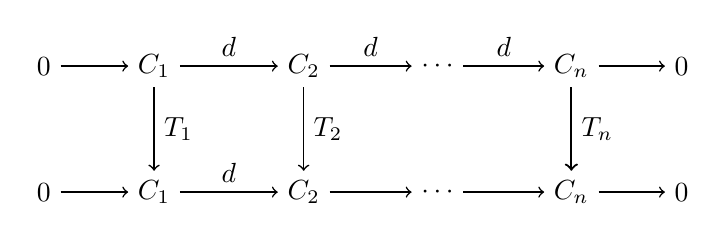
\begin{tikzpicture}[x=1cm,y=1cm]
\node(u0)at(0,0){$0$};\node(u1)at(1.4,0){$C_1$};\node(u2)at(3.3,0){$C_2$};
\node(ud)at(5,0){$\cdots$};\node(un)at(6.7,0){$C_n$};\node(uz)at(8.1,0){$0$};
\node(v0)at(0,-1.6){$0$};\node(v1)at(1.4,-1.6){$C_1$};\node(v2)at(3.3,-1.6){$C_2$};
\node(vd)at(5,-1.6){$\cdots$};\node(vn)at(6.7,-1.6){$C_n$};\node(vz)at(8.1,-1.6){$0$};
\draw[->,line width=.55pt](u0)--(u1);
\draw[->,line width=.55pt](u1)--node[above]{$d$}(u2);
\draw[->,line width=.55pt](u2)--node[above]{$d$}(ud);
\draw[->,line width=.55pt](ud)--node[above]{$d$}(un);
\draw[->,line width=.55pt](un)--(uz);
\draw[->,line width=.55pt](v0)--(v1);
\draw[->,line width=.55pt](v1)--node[above]{$d$}(v2);
\draw[->,line width=.55pt](v2)--(vd);
\draw[->,line width=.55pt](vd)--(vn);
\draw[->,line width=.55pt](vn)--(vz);
\draw[->,line width=.6pt](u1)--node[right]{$T_1$}(v1);
\draw[->,line width=.6pt](u2)--node[right]{$T_2$}(v2);
\draw[->,line width=.8pt](un)--node[right]{$T_n$}(vn);
\end{tikzpicture}\end{center}
\SourceFigure{GELFAND-P000106}{linear-algebra-diagram}{Две горизонтальные цепочки, крайние 0. В верхней три внутренних надписи d; в нижней d только между $C_1$ и $C_2$. Три вертикальных знака вниз, с $T_1$, $T_2$, $T_n$. У правого знака густой ромбовидный нижний конец; под ним нижний $C_n$ густо переписан. Наборное воссоздание сохраняет направление и надписи; густые контуры не разделены.}
\end{GelfandAdjacentEvidence}
\begin{GelfandAdjacentEvidence}{GELFAND-P000106}{99}

\begin{equation*}\frac{\operatorname{Ker}d|C_i}{\operatorname{Im}C_{i-1}}=H^i.\end{equation*}
\SourceFigure{GELFAND-P000106}{cohomology-quotient}{В рукописи дробная черта наклонная. Наверху Ker $d|C_i$, внизу плотное Im $C_{i-1}$; отдельного d и вертикальной черты после Im не видно. Справа $=H^i$.}
\end{GelfandAdjacentEvidence}
\begin{GelfandAdjacentEvidence}{GELFAND-P000106}{100}

$T_i^*:H^i\longrightarrow H^i$.
\begin{equation*}\sum(-1)^i\operatorname{tr}T_i=\sum(-1)^i\operatorname{tr}(T_i^*).\end{equation*}
\SourceFigure{GELFAND-P000106}{final-traces}{Слева $T_i^*:H^i\longrightarrow H^i$. В последнем равенстве у обеих сумм верхние i у $(-1)$; слева tr $T_i$, справа tr($T_i^*$).}
\end{GelfandAdjacentEvidence}
\begin{GelfandAdjacentEvidence}{GELFAND-P000107}{101}



\SourcePage{GELFAND-P000107}{70}
[Вверху зачёркнуто: Это[?] $C^\infty$ что[?]; остальное неразборчиво.]
\Unclear{GELFAND-P000107}{top-cancel}{Сквозь верхнюю строку проведён длинный штрих; под ним слева плотная запись, в середине $C^\infty$, справа что[?]. Границы и точное чтение слов не установлены.}
\end{GelfandAdjacentEvidence}
\begin{GelfandAdjacentEvidence}{GELFAND-P000107}{102}

Это кон. аналог.
\par\underline{Приложения.}
\par 1. Обычная формула Лефшеца.
$X\overset{f}{\longrightarrow}X$ изол. особ. точки.
Комплекс де Рама.
[Справа:]
\begin{gather*}
\bigl(\sum\text{ кратн. неподв. точек}\,=\\
=\sum\text{ следов на когом.}
\end{gather*}
\SourceFigure{GELFAND-P000107}{opening-applications}{Это кон. аналог. записано отдельно от зачёркнутой строки. Приложения. подчёркнуто. Справа открывающая скобка перед суммой; знак равенства в конце верхней строки и ещё один в начале нижней. Закрывающая скобка не видна.}
\end{GelfandAdjacentEvidence}
\begin{GelfandAdjacentEvidence}{GELFAND-P000107}{103}

\begin{equation*}
\underline{\operatorname{tr}\varphi_i(\rho)=\operatorname{det}-1}\,;
\end{equation*}
(счит. по соб. знач.)
\Unclear{GELFAND-P000107}{de-rham-determinant}{После det горизонтальный минус и знак 1-подобного начертания; чтения $-1$ / $-I$ и неразобранный аргумент остаются неразличёнными. Под всей записью длинная черта с загибом справа вверх.}
\end{GelfandAdjacentEvidence}
\begin{GelfandAdjacentEvidence}{GELFAND-P000107}{104}

[Справа:]
\begin{equation*}\sum\pm1\quad\text{по неподв. точкам}.\end{equation*}
\begin{equation*}
\sum(\pm1)\lambda_{i_1}\cdots\lambda_{i_k}\qquad
J_\rho=\begin{pmatrix}\lambda_1&&0\\&\ddots&\\0&&\lambda_n\end{pmatrix}
\end{equation*}
[Между $\lambda_1$ и $\lambda_n$ в матрице — диагональное многоточие.]
\SourceFigure{GELFAND-P000107}{exterior-trace-matrix}{У суммы отдельный знак $(\pm1)$, затем $\lambda_{i_1}\cdots\lambda_{i_k}$. Справа J-подобная буква с нижним $\rho$; в скобках $\lambda_1$ сверху слева, $\lambda_n$ снизу справа, нули в остальных углах и диагональное многоточие между ними.}
\end{GelfandAdjacentEvidence}
\begin{GelfandAdjacentEvidence}{GELFAND-P000107}{105}

\par 2. Комплексный случай.
$f:X\longrightarrow X$ — голом.
\begin{equation*}\sum f_{i_1\cdots i_k}\,dz_{i_1}\wedge\cdots\wedge dz_{i_k}\end{equation*}
$f_{i_1\cdots i_k}$ голом. и голом. дифф. $H^{i,0}($
\begin{flushright}\begin{tikzpicture}[x=1cm,y=1cm]
\draw[line width=.55pt](0,1.8)--(0,-.15);
\draw[line width=.55pt](0,0)--(1.4,0);
\end{tikzpicture}\end{flushright}
\SourceFigure{GELFAND-P000107}{complex-forms-corner}{Справа от строк форм длинный вертикальный штрих вниз и от него горизонтальный штрих вправо; стрелок и подписей у угла нет. У $H^{i,0}($ скобка остаётся открытой.}
\end{GelfandAdjacentEvidence}
\begin{GelfandAdjacentEvidence}{GELFAND-P000107}{106}

[Под $H^{i,0}($ густо зачёркнуто: неразборчиво.]
\Unclear{GELFAND-P000107}{holomorphic-cancel}{Ниже открытой скобки плотные горизонтальные штрихи с наклоном вверх вправо; отдельные буквы не различены.}
\end{GelfandAdjacentEvidence}
\begin{GelfandAdjacentEvidence}{GELFAND-P000107}{107}

\begin{equation*}
\sum(-1)^i\frac{\operatorname{tr}\varphi(E_i)}{|(1-J(f))|^2}=
\end{equation*}
[Зачёркнуто: $\sum_\rho\operatorname{Re}($; далее:]
\begin{equation*}\sum_\rho\operatorname{Re}\left(\frac{2}{1-J_f}\right)\end{equation*}
\Unclear{GELFAND-P000107}{complex-denominator}{Вертикальные штрихи у знаменателя утолщены: модуль / двойные штрихи. Внутри J-подобная буква / рукописное Д; у действующей суммы справа в числителе 2, под ней две близкие горизонтальные черты.}
\end{GelfandAdjacentEvidence}
\begin{GelfandAdjacentEvidence}{GELFAND-P000107}{108}

\begin{center}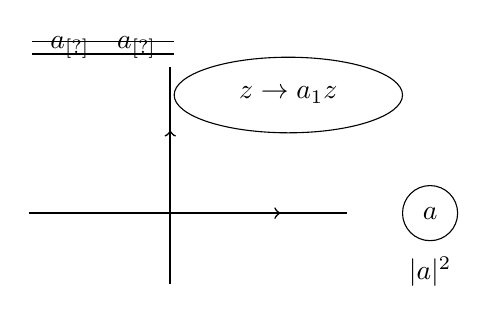
\begin{tikzpicture}[x=1cm,y=1cm]
\draw[line width=.6pt](-1.8,0)--(2.25,0);
\draw[->,line width=.6pt](0,0)--(1.4,0);
\draw[line width=.6pt](0,-.9)--(0,1.85);
\draw[->,line width=.6pt](0,0)--(0,1.05);
\node at(1.5,1.5){$z\to a_1z$};
\draw(1.5,1.5)ellipse(1.45cm and .48cm);
\node at(3.3,0){$a$};\draw(3.3,0)circle(.35cm);
\node at(3.3,-.75){$|a|^2$};
\node at(-.85,2.1){$a_{[?]}\quad a_{[?]}$};
\draw[line width=.7pt](-1.75,2.18)--(.05,2.18);
\draw[line width=.7pt](-1.75,2.02)--(.05,2.02);
\end{tikzpicture}\end{center}
\Unclear{GELFAND-P000107}{complex-axes}{Две пересекающиеся линии, стрелки вверх и вправо; горизонталь продолжается за наконечник. В овале $z\to a_1z$, отдельно в кружке a, ниже $|a|^2$. Над вертикалью зачёркнуты a-подобные знаки с нижними неразборчивыми штрихами; точное чтение этой записи не установлено.}
\end{GelfandAdjacentEvidence}
\begin{GelfandAdjacentEvidence}{GELFAND-P000107}{109}

Когда преобр. $\Vert$ дробно-лин., то это теор. о неподв. точке.
\SourceFigure{GELFAND-P000107}{mobius-statement}{Между преобр. и дробно-лин. две вертикальные черты. Последние слова неподв. точке. на следующей строке.}
\end{GelfandAdjacentEvidence}
\begin{GelfandAdjacentEvidence}{GELFAND-P000107}{110}

\begin{equation*}
=\frac{1}{[?]}\left(\frac{1}{\overline{1-J(f)}}+\frac{1}{1-J(f)}\right)
\end{equation*}
\Unclear{GELFAND-P000107}{conjugate-average}{Под первой отдельной 1 густой знак: 2[?] / 1[?] / неразборчиво. У первой внутренней дроби две длинные горизонтальные черты, у второй одна; первая дополнительная черта может относиться к сопряжению дроби или знаменателя.}
\end{GelfandAdjacentEvidence}
\begin{GelfandAdjacentEvidence}{GELFAND-P000107}{111}

Действ. след, есть [зачёркнуто: неразборчиво] сумма следов компл. и компл. сопр.
\Unclear{GELFAND-P000107}{real-trace-cancel}{Между есть и сумма густая горизонтальная зачёркнутая запись с вертикальным штрихом справа; отдельные буквы не различены.}
\end{GelfandAdjacentEvidence}
\begin{GelfandAdjacentEvidence}{GELFAND-P000107}{112}

Прим. и к [густо переписано: неразборчиво] преобр. проект. \underline{пр-ва} др-лин.
\Unclear{GELFAND-P000107}{projective-cancel}{После и к два плотных наложенных знака. Под сокращением пр-ва две отдельные короткие черты; предшествующая переписанная запись не разобрана.}
\end{GelfandAdjacentEvidence}
\begin{GelfandAdjacentEvidence}{GELFAND-P000107}{113}

\par\underline{Каждан.} \underline{Определение} \underline{гомологий} \underline{чего-угодно.}
\SourceFigure{GELFAND-P000107}{kazhdan-heading}{Фамилия и три части заголовка подчёркнуты отдельными чертами. Между чего и угодно дефис.}
\end{GelfandAdjacentEvidence}
\begin{GelfandAdjacentEvidence}{GELFAND-P000107}{114}

$C$ — абелева категория. объект $Q$ наз. инъективным, если функтор $F(A)=\operatorname{Hom}(A,Q)$ точен.
($A'\subset A$ $\forall f$ [зачёркнуто: неразборчивое слово] продолжается)
\begin{center}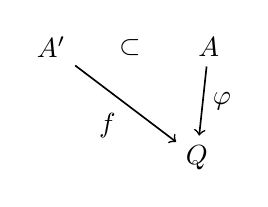
\begin{tikzpicture}[x=1cm,y=1cm]
\node(ap)at(0,0){$A'$};\node at(1,0){$\subset$};\node(a)at(2,0){$A$};
\node(q)at(1.85,-1.4){$Q$};
\draw[->,line width=.6pt](ap)--node[below left]{$f$}(q);
\draw[->,line width=.6pt](a)--node[right]{$\varphi$}(q);
\end{tikzpicture}\end{center}
\SourceFigure{GELFAND-P000107}{injective-definition-diagram}{Внутри скобок $A'\subset A$; от $A'$ стрелка вниз вправо с f, от A вниз к Q стрелка с $\varphi$ справа. У $F(A)$ верхнего индекса нет.}
\end{GelfandAdjacentEvidence}
\begin{GelfandAdjacentEvidence}{GELFAND-P000107}{115}

\Unclear{GELFAND-P000107}{extension-cancel}{После $\forall f$ над продолжается плотное зачёркнутое слово; его буквы не разделены.}
\end{GelfandAdjacentEvidence}
\begin{GelfandAdjacentEvidence}{GELFAND-P000107}{116}

В катег. дост. кол-во инъект. объектов, если $\forall A$ $\exists$ ин. $Q$ $\Vert$ $0\longrightarrow A\longrightarrow Q$.
[кат. пучков]
\SourceFigure{GELFAND-P000107}{enough-injectives}{Перед $0\to A\to Q$ две вертикальные черты, нижняя часть утолщена. Справа отдельная запись в квадратных скобках кат. пучков.}
\end{GelfandAdjacentEvidence}
\begin{GelfandAdjacentEvidence}{GELFAND-P000107}{117}

Пусть есть [зачёркнуто: неразборчиво] функтор $F(A)$ $C\overset{F}{\longrightarrow}C'$ ковар. и точный слева, т.е.

\begin{equation*}
0\longrightarrow A\longrightarrow B\longrightarrow\underbrace{C\longrightarrow0}_{\text{можно и не ставить.}}
\Longrightarrow0\longrightarrow F(A)\longrightarrow F(B)\longrightarrow F(C)
\end{equation*}
\Unclear{GELFAND-P000107}{functor-cancel}{Между есть и функтор маленькая плотная зачёркнутая запись, с выступающим вниз штрихом; точное чтение не установлено.}
\end{GelfandAdjacentEvidence}
\begin{GelfandAdjacentEvidence}{GELFAND-P000107}{118}


\SourceFigure{GELFAND-P000107}{functor-left-exact}{У $C\to C'$ над стрелкой F. Под $C\to0$ в исходной последовательности дуга с можно и не ставить. В последовательности после большой стрелки последний видимый член $F(C)$, затем точки или нуля нет.}
\end{GelfandAdjacentEvidence}
\begin{GelfandAdjacentEvidence}{GELFAND-P000107}{119}

и в $C$ дост. число инъект. об.
Производные функторы (они $\exists$ и ед.) — функторы из кат. $C$ в $C'$, удовл. условиям:
\par 1) $F^0(A)=F(A)$
\par 2) $F^{[?]}(Q)=0$ $(i>0)$ $\forall$ инъективного $Q$
\Unclear{GELFAND-P000107}{derived-conditions}{В условии 1 верхний знак 0. В условии 2 верхний знак над F залит и с небольшим выступом вверх: i[?] / 0[?] / неразборчиво; справа отдельно $(i>0)$.}
\end{GelfandAdjacentEvidence}
\begin{GelfandAdjacentEvidence}{GELFAND-P000107}{120}

\par 3) $\forall$ точн. послед. $0\longrightarrow A\longrightarrow B\longrightarrow C\longrightarrow0$ имеет место точн. послед.
\begin{equation*}
0\longrightarrow F^0(A)\longrightarrow F^0(B)\longrightarrow F^0(C)
\overset{\delta}{\longrightarrow}F^1(A)\longrightarrow F^1(B)\overset{\delta}{\longrightarrow}{}
\end{equation*}
\SourceFigure{GELFAND-P000107}{derived-long-sequence}{Внизу последовательность начинается 0, затем три члена с верхним 0, затем стрелка с $\delta$, два члена с верхним 1 и ещё одна стрелка с $\delta$.}
\end{GelfandAdjacentEvidence}
\begin{GelfandAdjacentEvidence}{GELFAND-P000107}{121}

\Incomplete{GELFAND-P000107}{derived-edge}{Последняя стрелка у правого края; следующий член на этом кадре не виден.}
\end{GelfandAdjacentEvidence}
\begin{GelfandAdjacentEvidence}{GELFAND-P000107}{122}

[Над последними стрелками: индуц[?] с продолжающимся вправо штрихом.]
\Unclear{GELFAND-P000107}{induced-annotation}{Читается индуц.[?] / индуц...[?]; окончание слито с длинным штрихом вправо, оканчивающимся рядом с последним $\delta$. Точное прикрепление штриха не установлено.}
\end{GelfandAdjacentEvidence}
\begin{GelfandAdjacentEvidence}{GELFAND-P000108}{123}


\usetikzlibrary{decorations.pathmorphing}

\SourcePage{GELFAND-P000108}{unlabelled}
Причем 3') Пусть есть другая точн. послед. и отобр.
\begin{center}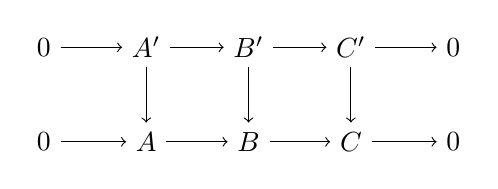
\begin{tikzpicture}[x=1cm,y=1cm]
\node(a0)at(0,0){$0$};\node(a1)at(1.3,0){$A'$};\node(a2)at(2.6,0){$B'$};\node(a3)at(3.9,0){$C'$};\node(a4)at(5.2,0){$0$};
\node(b0)at(0,-1.2){$0$};\node(b1)at(1.3,-1.2){$A$};\node(b2)at(2.6,-1.2){$B$};\node(b3)at(3.9,-1.2){$C$};\node(b4)at(5.2,-1.2){$0$};
\draw[->](a0)--(a1);\draw[->](a1)--(a2);\draw[->](a2)--(a3);\draw[->](a3)--(a4);
\draw[->](b0)--(b1);\draw[->](b1)--(b2);\draw[->](b2)--(b3);\draw[->](b3)--(b4);
\draw[->](a1)--(b1);\draw[->](a2)--(b2);\draw[->](a3)--(b3);
\end{tikzpicture}\end{center}
\SourceFigure{GELFAND-P000108}{exact-sequence-diagram}{Две строки $0\to A'\to B'\to C'\to0$ и $0\to A\to B\to C\to0$; три вертикальные стрелки от штрихованных букв вниз. У стрелок подписей нет.}
\end{GelfandAdjacentEvidence}
\begin{GelfandAdjacentEvidence}{GELFAND-P000108}{124}

\begin{center}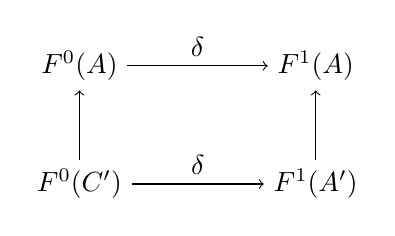
\begin{tikzpicture}[x=1cm,y=1cm]
\node(a)at(0,0){$F^0(A)$};\node(b)at(3,0){$F^1(A)$};
\node(c)at(0,-1.5){$F^0(C')$};\node(d)at(3,-1.5){$F^1(A')$};
\draw[->](a)--node[above]{$\delta$}(b);\draw[->](c)--node[above]{$\delta$}(d);
\draw[->](c)--(a);\draw[->](d)--(b);
\end{tikzpicture}\end{center}
\Unclear{GELFAND-P000108}{connecting-square-label}{В верхнем левом углу $F^0(A)$: видны две наклонные стороны и поперечный штрих A. Верхний правый $F^1(A)$, нижние $F^0(C')$ и $F^1(A')$; обе вертикальные стрелки направлены вверх.}
\end{GelfandAdjacentEvidence}
\begin{GelfandAdjacentEvidence}{GELFAND-P000108}{125}

\underline{Теорема}: Если в $A$ дост. число инъект. об., то произв. функторы сущ. и ед.
\SourceFigure{GELFAND-P000108}{theorem}{В условии после в отдельная большая A. Теорема подчёркнуто, двоеточие справа от черты. Сущ. и ед. продолжают запись на следующей строке.}
\end{GelfandAdjacentEvidence}
\begin{GelfandAdjacentEvidence}{GELFAND-P000108}{126}

\par $15/\underline{\overline{\mathrm{XI}}}$ \underline{Мацаев} \tikz[baseline=(title.base)]{\node[inner sep=0pt](title){Полное док-во теор. Атья-Ботта.};\draw[decorate,decoration={snake,amplitude=.45pt,segment length=5pt}] ([yshift=-2pt]title.south west)--([yshift=-2pt]title.south east);}
\SourceFigure{GELFAND-P000108}{matsaev-heading}{У XI черты сверху и снизу. Под фамилией прямая черта; под Полное док-во теор. Атья-Ботта. волнистая черта.}
\end{GelfandAdjacentEvidence}
\begin{GelfandAdjacentEvidence}{GELFAND-P000108}{127}

\begin{equation*}\cdots\longrightarrow\Gamma(E_i)\overset{d}{\longrightarrow}\Gamma(E_{i+1})\longrightarrow\cdots\end{equation*}
Даны $T$, действ. в $\Gamma$ и коммут. с $d$, $T_i^*$,
\SourceFigure{GELFAND-P000108}{bundle-complex}{В комплексе над средней стрелкой d, справа индекс $i+1$. В следующей строке $T_i^*$, после него запятая.}
\end{GelfandAdjacentEvidence}
\begin{GelfandAdjacentEvidence}{GELFAND-P000108}{128}

[Густо зачёркнуто: неразборчивый знак; справа T-подобный знак[?].]
\Unclear{GELFAND-P000108}{operator-cancel}{Плотная зачёркнутая запись наклонена вверх вправо; правее отдельный небольшой знак с горизонтальным верхом и наклонной ножкой: T[?] / неразборчиво.}
\end{GelfandAdjacentEvidence}
\begin{GelfandAdjacentEvidence}{GELFAND-P000108}{129}

\begin{equation*}L(T,E)=\sum(-1)^i\operatorname{tr}T_i^*\end{equation*}
[Справа:] (Здесь $z$ нам не нужно — не зависит)
\SourceFigure{GELFAND-P000108}{L-and-parameter}{У T в сумме верхний знак звёздочка и нижний i. В правой скобке z, затем нам не нужно, внизу — не зависит.}
\end{GelfandAdjacentEvidence}
\begin{GelfandAdjacentEvidence}{GELFAND-P000108}{130}

\begin{equation*}\sum_i\sigma(\rho)\qquad\sigma(\rho)=\sum\frac{(-1)^i\operatorname{Sp}\varphi_i(\rho)}{|\operatorname{det}(1-I_f(\rho))|}\end{equation*}
\Unclear{GELFAND-P000108}{fixed-point-index}{Под первой суммой маленький знак с отдельной точкой сверху: i[?] / неразборчивый индекс. В знаменателе буква I-подобная с широким основанием / J-подобная; после неё нижний f и $(\rho)$.}
\end{GelfandAdjacentEvidence}
\begin{GelfandAdjacentEvidence}{GELFAND-P000108}{131}

Формальное док-во тривиально, т.к.
\begin{equation*}L=\sum_i(-1)^i\operatorname{tr}T_i\end{equation*}
(элем. теор. лин. алгебры)
$\operatorname{tr}T_i$ формально дают эту сумму.
$T_i$ зад. ядром $\varphi\delta(y-f(x))$. След как раз $\sum$ по неподв. точкам.
\SourceFigure{GELFAND-P000108}{formal-trace-kernel}{В формальной сумме у T нижний i без звёздочки. В ядре после y горизонтальный минус, затем $f(x)$. Неподв. точкам. перенесено на следующую строку.}
\end{GelfandAdjacentEvidence}
\begin{GelfandAdjacentEvidence}{GELFAND-P000108}{132}

Смаж. ядром
\begin{equation*}(1+\Box)^{-z}T_i=T_{i,z},\qquad\Box=d\delta+\delta d\end{equation*}
(счит. зад. рим. метр., эр. сопр. опер.)
[Зачёркнуто: $(1+\Box)^{-z}$.]
След. уже сущ. в обычн. смысле.
\SourceFigure{GELFAND-P000108}{smoothing-metric}{В показателе $-z$; у правого $T_{i,z}$ запятая. Отдельная формула с квадратом, d и $\delta$. Ниже зачёркнутая копия $(1+\Box)^{-z}$.}
\end{GelfandAdjacentEvidence}
\begin{GelfandAdjacentEvidence}{GELFAND-P000108}{133}

\begin{equation*}\operatorname{tr}T_{iz}=\sum_\lambda\pi_\lambda T i_\lambda(1+\lambda)^{-z}\end{equation*}
\Unclear{GELFAND-P000108}{trace-series-overwrite}{Индексы у левого T густо переписаны: iz / i,z. Справа $\pi_\lambda$, T, $i_\lambda$ и $(1+\lambda)^{-z}$; отдельного tr после суммы не видно.}
\end{GelfandAdjacentEvidence}
\begin{GelfandAdjacentEvidence}{GELFAND-P000108}{134}

$\sum_i(-1)^i\operatorname{tr}T_{iz}$ продолж. на всю плоскость и при $z=0$ есть интегр. как число.
\SourceFigure{GELFAND-P000108}{analytic-continuation}{В сумме нижний i, после слов всю плоскость и продолжение при $z=0$ есть интегр. как число.}
\end{GelfandAdjacentEvidence}
\begin{GelfandAdjacentEvidence}{GELFAND-P000108}{135}

\begin{equation*}T_{iz}=\underbrace{(1+\Box)^{-z}}_{\text{он зад. интегральным ядром при дост. большой }\operatorname{Re}z}\,T_i\end{equation*}
\SourceFigure{GELFAND-P000108}{integral-kernel-annotation}{Под $(1+\Box)^{-z}$ прямая скобка с коротким штрихом вниз; пояснение под ней оканчивается $\operatorname{Re}z$.}
\end{GelfandAdjacentEvidence}
\begin{GelfandAdjacentEvidence}{GELFAND-P000108}{136}

и это ядро устроено так: [зачёркнуто: неразборчивое слово]
\Unclear{GELFAND-P000108}{kernel-cancel}{После устроено так: две плотные почти горизонтальные зачёркивающие черты; исходные буквы не разделены.}
\end{GelfandAdjacentEvidence}
\begin{GelfandAdjacentEvidence}{GELFAND-P000108}{137}

\begin{center}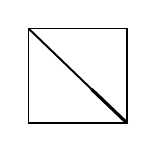
\begin{tikzpicture}[x=1cm,y=1cm]
\draw[line width=.6pt](0,0)--(0,1.2)--(1.25,1.2)--(1.25,0)--cycle;
\draw[line width=.7pt](0,1.2)--(.8,.43);
\draw[line width=1.15pt](.8,.43)--(1.25,0);
\end{tikzpicture}\end{center}
\Unclear{GELFAND-P000108}{diagonal-kernel}{Квадрат без подписей; диагональ идёт от верхнего левого угла к нижнему правому и у последнего утолщается. Утолщение / наконечник стрелки[?]; отдельной подписи у него нет.}
\end{GelfandAdjacentEvidence}
\begin{GelfandAdjacentEvidence}{GELFAND-P000108}{138}

вне диаг. ядро $C^\infty$, а на диаг. изломы производной (контр.[?] Катцу и Нарасимхан)
\Unclear{GELFAND-P000108}{kernel-description-names}{В скобке сокращение контр.[?] с плотным концом, затем Катцу и Нарасимхан. Перед скобкой производной.}
\end{GelfandAdjacentEvidence}
\begin{GelfandAdjacentEvidence}{GELFAND-P000108}{139}

Речь идёт о $(1+\Box)^{-z}$ (без $T_i$).
\SourceFigure{GELFAND-P000108}{kernel-family}{В последней скобке без $T_i$. До неё отдельное $(1+\Box)^{-z}$.}
\end{GelfandAdjacentEvidence}
\begin{GelfandAdjacentEvidence}{GELFAND-P000108}{140}

\begin{equation*}\mu_1(x)(1+\Box)^{-z}\mu_2(x)\end{equation*}
уже зад. $C^\infty$-ядром, если $\operatorname{supp}[?]\,\mu_1\,\mu_2$ на краях.
\Unclear{GELFAND-P000108}{kernel-localization}{Крайние буквы $\mu_1,\mu_2$ / $M_1,M_2$; первый знак более угловат. После если supp[?] / дифф[?] / неразборчиво; ниже на краях. Между двумя буквами после сокращения точный разделительный знак не различим.}
\end{GelfandAdjacentEvidence}
\begin{GelfandAdjacentEvidence}{GELFAND-P000109}{141}



\SourcePage{GELFAND-P000109}{71}
\begin{center}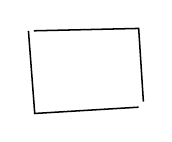
\begin{tikzpicture}[x=1cm,y=1cm]
\draw[line width=.55pt](0,1.05)--(.08,0)--(1.40,.08);
\draw[line width=.55pt](.07,1.05)--(1.40,1.08)--(1.46,.15);
\end{tikzpicture}\end{center}
\SourceFigure{GELFAND-P000109}{empty-square}{Пустой четырёхугольник в левом верхнем поле; без диагонали и подписей. Справа внизу концы сторон не соединены; небольшой промежуток также слева вверху.}
\end{GelfandAdjacentEvidence}
\begin{GelfandAdjacentEvidence}{GELFAND-P000109}{142}

Когда можно корректно перемножить две обобщ. ф-и с особенностями на двух трансверсальных мн-зиях.
\SourceFigure{GELFAND-P000109}{opening-question}{Запись начинается Когда и оканчивается мн-зиях. Знака вопроса в конце нет.}
\end{GelfandAdjacentEvidence}
\begin{GelfandAdjacentEvidence}{GELFAND-P000109}{143}

$\mu_1,\mu_2$ [зачёркнуто: неразборчиво]

$\cap$ нос. вне кривой[?], то [зачёркнуто: неразборчиво]

ф-я зад. ф-ей.
\Unclear{GELFAND-P000109}{support-first-cancel}{Между $\mu_1,\mu_2$ и $\cap$ короткая густо зачёркнутая запись. У первой буквы $\mu$ угловатый верх и длинный нижний штрих.}
\end{GelfandAdjacentEvidence}
\begin{GelfandAdjacentEvidence}{GELFAND-P000109}{144}

\Unclear{GELFAND-P000109}{support-second-cancel}{После то и перед ф-я плотная зачёркнутая запись; исходные знаки не разделены.}
\end{GelfandAdjacentEvidence}
\begin{GelfandAdjacentEvidence}{GELFAND-P000109}{145}

\Unclear{GELFAND-P000109}{support-condition-word}{Вне кривой[?] / вне прямой: начальная буква последнего слова плотная, следующая имеет длинный нижний штрих.}
\end{GelfandAdjacentEvidence}
\begin{GelfandAdjacentEvidence}{GELFAND-P000109}{146}



\usetikzlibrary{decorations.pathmorphing}
\tikz[baseline=(title.base)]{\node[inner sep=0pt](title){Достат. условие};\draw[decorate,decoration={snake,amplitude=.45pt,segment length=5pt}]([yshift=-2pt]title.south west)--([yshift=-2pt]title.south east);}: каждая из них гладкая $\delta$-ф-я, а к ней примен. оператор $P\delta_S$, если $P$ — псевдодифф. (например, просто дифф.)
\SourceFigure{GELFAND-P000109}{delta-sufficient}{Под Достат. условие волнистая черта. После оператор отдельное $P\delta_S$; далее если $P$ — псевдодифф. Скобка заканчивается просто дифф.)}
\end{GelfandAdjacentEvidence}
\begin{GelfandAdjacentEvidence}{GELFAND-P000109}{147}

К ней можно применить [густо зачёркнуто: неразборчивый знак]

псевдодифф. оператор.
\Unclear{GELFAND-P000109}{pseudo-cancel}{Между применить и псевдодифф. короткий плотный знак с нижним наклонным штрихом.}
\end{GelfandAdjacentEvidence}
\begin{GelfandAdjacentEvidence}{GELFAND-P000109}{148}


Гладкая ф-я на мн-зии — $\int$ по мн-зию.
Это непр. опер. на $C^\infty$ ф-ях и значит на обобщ. ф-ях.
Надо приблизить $\delta$-ф-и $C^\infty$-ф-ями спец. образом, тогда произвед. будет иметь предел.
\SourceFigure{GELFAND-P000109}{distribution-action}{После тире отдельный знак интеграла без пределов. Затем две фразы о непр. опер. и приближении $\delta$-ф-и; в конце предел.}
\end{GelfandAdjacentEvidence}
\begin{GelfandAdjacentEvidence}{GELFAND-P000109}{149}

\begin{equation*}\delta(x_1)\cdot\delta(x_2)=\delta(x_1,x_2)\end{equation*}
\SourceFigure{GELFAND-P000109}{delta-product}{Между первыми двумя множителями точка; справа $\delta(x_1,x_2)$ без отдельной конечной точки.}
\end{GelfandAdjacentEvidence}
\begin{GelfandAdjacentEvidence}{GELFAND-P000109}{150}

\begin{center}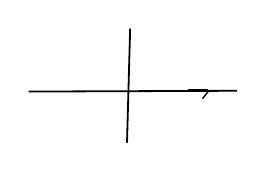
\begin{tikzpicture}[x=1cm,y=1cm]
\draw[line width=.65pt](-1.25,0)--(1.40,.01);
\draw[line width=.65pt](0,-.65)--(.04,.80);
\draw[line width=1.05pt](.78,.015)--(1.03,.015);
\draw[line width=.5pt](1.03,0)--(.96,-.09);
\end{tikzpicture}\end{center}
\Unclear{GELFAND-P000109}{transverse-lines}{Пересекающиеся вертикальная и горизонтальная линии без подписей. Правее пересечения короткое утолщение и наклонный штрих: наконечник стрелки[?] / неровность линии. Отдельно отмеченной точки нет.}
\end{GelfandAdjacentEvidence}
\begin{GelfandAdjacentEvidence}{GELFAND-P000109}{151}

(нос. в 4-хмерн. пр-ве трансверс. пересек. диаг.)
\SourceFigure{GELFAND-P000109}{diagonal-aside}{Скобка под формулой: нос. в 4-хмерн. пр-ве трансверс. пересек. диаг.}
\end{GelfandAdjacentEvidence}
\begin{GelfandAdjacentEvidence}{GELFAND-P000109}{152}


\underline{Каждан.} $X_P$ — откр. мн-во в топ. Зарисского. $P\ne0$.
\SourceFigure{GELFAND-P000109}{kazhdan-heading-open}{Фамилия Каждан. подчёркнута. Далее $X_P$, справа $P\ne0$.}
\end{GelfandAdjacentEvidence}
\begin{GelfandAdjacentEvidence}{GELFAND-P000109}{153}

[Слева зачёркнуто: неразборчивое слово.]
\Unclear{GELFAND-P000109}{kazhdan-cancel}{Ниже подчёркнутой фамилии и слева от Это базис несколько густых зачёркивающих штрихов.}
\end{GelfandAdjacentEvidence}
\begin{GelfandAdjacentEvidence}{GELFAND-P000109}{154}

Это базис откр. мн-в. на афф. алг. мн-зии.
Сеч. пучка на $X_P$: $R(x)$: $\dfrac{Q(x)}{P^n}$,

[Зачёркнут короткий знак: $=$[?] / неразборчиво.]

они отожд., если разн. обр. в 0 на мн-зии.
\SourceFigure{GELFAND-P000109}{sections-quotient}{После $X_P$ и после $R(x)$ двоеточия. Числитель $Q(x)$, знаменатель $P^n$; справа запятая.}
\end{GelfandAdjacentEvidence}
\begin{GelfandAdjacentEvidence}{GELFAND-P000109}{155}

\Unclear{GELFAND-P000109}{quotient-cancel}{Перед они короткий тёмный знак с двумя почти горизонтальными штрихами; исходный знак $=$[?].}
\end{GelfandAdjacentEvidence}
\begin{GelfandAdjacentEvidence}{GELFAND-P000109}{156}


$\Gamma(X_P,O_X)$. Афф. алг. мн. — конечн. число ур-й.
$X_P$ снова афф. пр-во.
\SourceFigure{GELFAND-P000109}{affine-descriptions}{После $\Gamma(X_P,O_X)$ точка. В последней строке именно снова афф. пр-во.}
\end{GelfandAdjacentEvidence}
\begin{GelfandAdjacentEvidence}{GELFAND-P000109}{157}


Алгебр. пучок — пучок модулей над этим пучком колец.
Конечн. типа — лок. изом. фактору прямой суммы.
\SourceFigure{GELFAND-P000109}{algebraic-finite-type}{Две строки: определение алгебр. пучка и запись Конечн. типа — лок. изом. фактору прямой суммы.}
\end{GelfandAdjacentEvidence}
\begin{GelfandAdjacentEvidence}{GELFAND-P000109}{158}

Когер. пучок — ещё $\forall$ [зачёркнуто: неразборчиво] откр. мн-ва и $\forall$ конечн. наб. сечений пучок соотн. конечного типа.
\Unclear{GELFAND-P000109}{coherent-cancel}{После первого $\forall$ густо зачёркнуто слово. Следом откр. мн-ва и $\forall$ конечн. наб.; продолжение на следующей строке сечений пучок соотн. конечного типа.}
\end{GelfandAdjacentEvidence}
\begin{GelfandAdjacentEvidence}{GELFAND-P000109}{159}

\underline{Теорема}: сам пучок $O$ когерентен.
\SourceFigure{GELFAND-P000109}{structure-coherent-theorem}{Теорема подчёркнуто, двоеточие справа. После сам пучок отдельное O, затем когерентен.}
\end{GelfandAdjacentEvidence}
\begin{GelfandAdjacentEvidence}{GELFAND-P000109}{160}


Сначала для всего афф. [зачёркнуто: мн-зии[?] / неразборчиво.] [Надписано: пр-ва.] Из этого всё получ. автом.
\Unclear{GELFAND-P000109}{variety-cancel}{Под вставкой пр-ва зачёркнутая запись мн-зии[?]. После неё точка; продолжение Из этого всё получ. на той же строке, автом. ниже.}
\end{GelfandAdjacentEvidence}
\begin{GelfandAdjacentEvidence}{GELFAND-P000109}{161}

$X_P$ — откр. мн-во. Рассм. конечн. набор сечений
\begin{equation*}\left(\frac{Q_1}{P^n},\frac{Q_2}{P^n},\ldots,\frac{Q_i}{P^n}\right)\end{equation*}
Пучок соотношений:
\SourceFigure{GELFAND-P000109}{localized-sections}{В кортеже нижние индексы $1,2,\ldots,i$, знаменатели $P^n$; после скобки отдельной точки нет. Справа Пучок соотношений:}
\end{GelfandAdjacentEvidence}
\begin{GelfandAdjacentEvidence}{GELFAND-P000109}{162}

Кольцо $A=k[x_1,\ldots,x_n]$. [Справа ещё: Пучок соотношений]
\SourceFigure{GELFAND-P000109}{relations-ring}{Кольцо $A=k[x_1,\ldots,x_n]$ с конечной точкой. Справа повторено Пучок соотношений без конечного знака.}
\end{GelfandAdjacentEvidence}
\begin{GelfandAdjacentEvidence}{GELFAND-P000109}{163}

\begin{equation*}O_X+O_X+\cdots+O_X\underset{\text{над }X_P}{\longrightarrow}O_X\end{equation*}
\SourceFigure{GELFAND-P000109}{sheaf-map}{Везде $O_X$; между первыми слагаемыми плюсы. Под направленной вправо стрелкой над $X_P$.}
\end{GelfandAdjacentEvidence}
\begin{GelfandAdjacentEvidence}{GELFAND-P000109}{164}

\begin{equation*}d_{3[?]}\ d_2\cdots d_i\longrightarrow\frac{d_1Q_1}{P^n}+\frac{d_2Q_2}{P^n}+\cdots+\frac{d_iQ_i}{P^n}\end{equation*}
\Unclear{GELFAND-P000109}{relation-first-subscript}{Первый нижний индекс слева похож на 3 / 1; нижний конец очень плотный. У первого $d$ справа индекс 1. Далее слева $d_2$, многоточие и $d_i$; точки в конце формулы нет.}
\end{GelfandAdjacentEvidence}
\begin{GelfandAdjacentEvidence}{GELFAND-P000109}{165}

Ядро — слой пучка соотн. над точкой
\SourceFigure{GELFAND-P000109}{kernel-stalk}{В последней строке слой, затем пучка соотн. над точкой. После последнего слова отдельного конечного знака нет.}
\end{GelfandAdjacentEvidence}
\begin{GelfandAdjacentEvidence}{GELFAND-P000110}{166}



\SourcePage{GELFAND-P000110}{unlabelled}
Рассм. след. отображение:
\begin{equation*}A+A+A+\cdots+A\longrightarrow A\end{equation*}
\SourceFigure{GELFAND-P000110}{opening-map}{После отображение двоеточие; у направленной вправо стрелки подписей нет. После последнего A отдельной точки нет.}
\end{GelfandAdjacentEvidence}
\begin{GelfandAdjacentEvidence}{GELFAND-P000110}{167}

Можно обойтись без $P$, соотн. те же самые,
Ядро — подмодуль, $A$ — нётерово, $d_1\cdots d_i$ и порождают [зачёркнуто: неразборчивый знак] пучок соотн. над любой точкой (теор. Гильберта)
\Unclear{GELFAND-P000110}{relations-prefix-cancel}{Слева перед пучок соотн. короткий зачёркнутый знак. В предыдущей строке $d_1$, многоточие, $d_i$ и порождают; правый конец последнего слова достигает края снимка.}
\end{GelfandAdjacentEvidence}
\begin{GelfandAdjacentEvidence}{GELFAND-P000110}{168}

[Зачёркнута вся строка: Из когер. кольца сл., что всякий пучок когер., то[?]; отдельные части неразборчивы.]
\Unclear{GELFAND-P000110}{whole-line-cancel}{Длинные штрихи пересекают всю строку. Чтение Из когер. кольца сл., что всякий пучок когер., то частичное; под густыми участками точные буквы не установлены.}
\end{GelfandAdjacentEvidence}
\begin{GelfandAdjacentEvidence}{GELFAND-P000110}{169}

Отсюда автом. след. когер. пучка $\forall$ афф. мн-зии.
$Y\subset X$, $Y$ — замкнуто, $O_X$ — на $X$, $J_Y$[?] — пучок идеалов ($=0$ на $Y$).
\SourceFigure{GELFAND-P000110}{closed-subvariety}{После когер. пучка отдельный $\forall$. В следующей строке $Y\subset X$, затем $Y$ — замкнуто.}
\end{GelfandAdjacentEvidence}
\begin{GelfandAdjacentEvidence}{GELFAND-P000110}{170}

Пучок на $Y$ по опр. $O_X/J_Y=O_Y$.
$O_Y$ тоже когер., т.к. ядро $J_Y$ — когер. пучок.
Структ. пучок на любом алг. мн-зии когерентен.
\Unclear{GELFAND-P000110}{quotient-and-kernel}{Буква идеала J[?] / I-подобная: сверху изогнутый штрих, внизу плотная петля. В формуле косая черта между $O_X$ и этой буквой с нижним Y; справа $=O_Y$. В следующей строке после ядро та же буква.}
\end{GelfandAdjacentEvidence}
\begin{GelfandAdjacentEvidence}{GELFAND-P000110}{171}

\usetikzlibrary{decorations.pathmorphing}
\tikz[baseline=(title.base)]{\node[inner sep=0pt](title){Свойства кольца сечений пучка $A$.};\draw[decorate,decoration={snake,amplitude=.45pt,segment length=5pt}]([yshift=-2pt]title.south west)--([yshift=-2pt]title.south east);}
\SourceFigure{GELFAND-P000110}{section-ring-heading}{Вся строка Свойства кольца сечений пучка A. подчёркнута волнистой чертой.}
\end{GelfandAdjacentEvidence}
\begin{GelfandAdjacentEvidence}{GELFAND-P000110}{172}

Отсюда когомологии любого когер. пучка на афф. мн-зии тривиальны. (Отсюда можно вычислять когом. с афф. покр. — — и наоборот — теор. Шевалле $H^i=0\Longrightarrow$
\Incomplete{GELFAND-P000110}{cohomology-chevalley}{После $H^i=0$ направленная вправо двойная стрелка; справа от неё продолжения нет. Открытая перед вторым Отсюда скобка не закрыта.}
\end{GelfandAdjacentEvidence}
\begin{GelfandAdjacentEvidence}{GELFAND-P000110}{173}

\begin{equation*}A=k[x_1,\ldots,x_n].\end{equation*}
Теор. Гильберта о нулях:
$J$ — идеал, $P$ — многочлен, обращ. в 0 на соотв. алг. мн-зии, тогда $P^k\in J$
\SourceFigure{GELFAND-P000110}{nullstellensatz}{У кольца $A=k[x_1,\ldots,x_n]$ конечная точка. После Теор. Гильберта о нулях двоеточие. У $P$ показатель k; после $J$ отдельной точки нет.}
\end{GelfandAdjacentEvidence}
\begin{GelfandAdjacentEvidence}{GELFAND-P000110}{174}

\usetikzlibrary{decorations.pathmorphing}
\tikz[baseline=(title.base)]{\node[inner sep=0pt](title){Следствие};\draw[decorate,decoration={snake,amplitude=.45pt,segment length=5pt}]([yshift=-2pt]title.south west)--([yshift=-2pt]title.south east);}. $A$ — кольцо сечений для любого афф. мн-зии.
\SourceFigure{GELFAND-P000110}{section-ring-consequence}{Под Следствие волнистая черта. Далее $A$ — кольцо сечений для любого афф. мн-зии.}
\end{GelfandAdjacentEvidence}
\begin{GelfandAdjacentEvidence}{GELFAND-P000110}{175}

Глоб. сеч. на всём [зачёркнуто: неразборчиво] афф. пр-ве — мног.[?] на всём пространстве.
\Unclear{GELFAND-P000110}{global-cancel}{Между всём и афф. короткая зачёркнутая запись; нижний правый конец образует петлю.}
\end{GelfandAdjacentEvidence}
\begin{GelfandAdjacentEvidence}{GELFAND-P000110}{176}

\Unclear{GELFAND-P000110}{global-word}{После тире сокращение мног.[?] / множ.; последний знак тесно связан с предыдущим. Сокращение не раскрыто.}
\end{GelfandAdjacentEvidence}
\begin{GelfandAdjacentEvidence}{GELFAND-P000110}{177}

\underline{Теор.} Любой пучок на афф. мн. [густой знак: неразборчиво] порожд. сеч. и когом. высш. разм. трив.
\Unclear{GELFAND-P000110}{theorem-mark}{Между мн. и порожд. густой отдельный знак с нижним штрихом. Слова когер. перед пучок в этой строке не видно.}
\end{GelfandAdjacentEvidence}
\begin{GelfandAdjacentEvidence}{GELFAND-P000110}{178}


\underline{Лемма 1.} $X$ — мн-зие (аффинное), $P$ — мног., $X_P=\{P\ne0\}$.
\SourceFigure{GELFAND-P000110}{lemma1-hypotheses}{Лемма 1. подчёркнуто прямой чертой. Аффинное в скобках. Справа $X_P=\{P\ne0\}$.}
\end{GelfandAdjacentEvidence}
\begin{GelfandAdjacentEvidence}{GELFAND-P000110}{179}

Над $X$ когер. пучок, [зачёркнуто: обращ. в 0 на $X_P$[?].] [Справа отдельно зачёркнуто: неразборчиво.]

и есть сечение $s$, обращ. в 0 на $X_P$. Тогда $\exists m$, что $P^ms=0$.
Это лёгкая переформул. теор. Гильберта.
\Unclear{GELFAND-P000110}{lemma-cancel}{После пучок длинные зачёркивающие штрихи; различимы части обращ., в 0, на $X_P$[?]. Правее отдельная плотная зачёркнутая запись.}
\end{GelfandAdjacentEvidence}
\begin{GelfandAdjacentEvidence}{GELFAND-P000110}{180}


\SourceFigure{GELFAND-P000110}{lemma1-section}{Незачёркнутая строка и есть сечение s, обращ. в 0 на $X_P$. Затем Тогда $\exists m$, что $P^ms=0$.}
\end{GelfandAdjacentEvidence}
\begin{GelfandAdjacentEvidence}{GELFAND-P000110}{181}


Пусть $X$ — афф. прямая
\begin{center}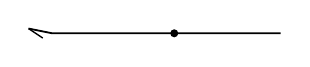
\begin{tikzpicture}[x=1cm,y=1cm]
\draw[line width=.65pt](-1.6,.06)--(-1.3,0)--(1.6,0);
\draw[line width=.5pt](-1.6,.06)--(-1.42,-.06);
\fill(.25,0)circle(1.45pt);
\end{tikzpicture}\end{center}
\Unclear{GELFAND-P000110}{affine-line}{Горизонтальная линия с выделенной точкой; подписи у точки нет. У левого конца короткий наклонный штрих вниз: наконечник влево[?] / изгиб линии. Справа наконечника не видно.}
\end{GelfandAdjacentEvidence}
\begin{GelfandAdjacentEvidence}{GELFAND-P000110}{182}

$k[x]$ — ростки мног., обр. в 0 в точке 0, фактор — одномерн.
\SourceFigure{GELFAND-P000110}{polynomial-germs}{Справа от рисунка $k[x]$ — ростки; на следующей строке мног., обр. в 0 в точке 0, фактор — одномерн.}
\end{GelfandAdjacentEvidence}
\begin{GelfandAdjacentEvidence}{GELFAND-P000110}{183}


\usetikzlibrary{decorations.pathmorphing}
\tikz[baseline=(title.base)]{\node[inner sep=0pt](title){Экзамен по гом. алгебре — по Гротендику.};\draw[decorate,decoration={snake,amplitude=.45pt,segment length=5pt}]([yshift=-2pt]title.south west)--([yshift=-2pt]title.south east);} — контр. работа.
\SourceFigure{GELFAND-P000110}{exam-heading}{Волнистая черта от Экзамен до Гротендику. После неё — контр., а работа. перенесено ниже без подчёркивания.}
\end{GelfandAdjacentEvidence}
\begin{GelfandAdjacentEvidence}{GELFAND-P000110}{184}

\underline{Лемма 2.} $F\subset O_X^{n[?]}$ — прямая $\sum$.
[Ниже со знаком вставки: подпучок.]
\Unclear{GELFAND-P000110}{lemma2-sum}{После прямая отдельный знак $\sum$ / $\Sigma$ с точкой справа. У $O_X$ верхний индекс n[?] / m-подобный; маленькие верхние штрихи слиты. Под F вставлено подпучок.}
\end{GelfandAdjacentEvidence}
\begin{GelfandAdjacentEvidence}{GELFAND-P000110}{185}

Пусть есть сечение $s$, опр. на $X_P$. Тогда при большом $m$ $P^ms$ продолжается на всё $X$.
\SourceFigure{GELFAND-P000110}{lemma2-extension}{Сечение s опр. на $X_P$. В последней строке $P^ms$ продолжается на всё X. В конце видна точка.}
\end{GelfandAdjacentEvidence}



\begin{GelfandAdjacentEvidence}{GELFAND-P000111}{1}
\SourcePage{GELFAND-P000111}{72}
(тоже теор. Гильберта).
\begin{equation*}\left(\frac{O_1\text{[?]}}{p^k},\ldots,\frac{O_i\text{[?]}}{p^k}\right)\end{equation*}
умн. на $p^k$, но это может не быть сеч. $O_X^n$.
\Unclear{GELFAND-P000111}{opening-numerators}{В числителях округлые O-подобные знаки с нижними $1$ и $i$; нижние части сливаются с дробными чертами. Чтения $O$ / $Q$ не вполне разделены. Ниже $O_X^n$ и $O_X^n/F$.}
\end{GelfandAdjacentEvidence}
\begin{GelfandAdjacentEvidence}{GELFAND-P000111}{2}

$O_X^n/F\longrightarrow0$ уже непр.[?]
\Unclear{GELFAND-P000111}{quotient-last-word}{После уже короткая связная запись непр.[?]; средние и конечные штрихи густо слиты. Сокращение не раскрыто. Перед уже стрелка к отдельному $0$.}
\end{GelfandAdjacentEvidence}
\begin{GelfandAdjacentEvidence}{GELFAND-P000111}{3}

Теперь уже дост. для док-ва то, что когом. $F\subset O_X^n$ нули.
$X$ — афф. мн., $(X_{p_1},X_{p_2},\ldots,X_{p_i})$ покр.
Когомологии $X$ с коэфф. в $F$ в этом покр. нули.

$22/\underline{\overline{XI}}$. \underline{И.М. Гельфанд.}
[Зачёркнуто: неразборчивая запись.] Bott, Chern Acta Math., 1965, \underline{114} $N=1$–$2$.
\Unclear{GELFAND-P000111}{bott-name-cancel}{Перед Bott густо зачёркнута запись с Б-подобным началом; отдельные прежние буквы не установлены. После отмены отдельная запятая.}
\end{GelfandAdjacentEvidence}
\begin{GelfandAdjacentEvidence}{GELFAND-P000111}{4}

\noindent\tikz[baseline=(title.base)]{\node[inner sep=0pt,outer sep=0pt](title){Теории Неванлинны для многих переменных.};\draw[decorate,decoration={snake,amplitude=.35mm,segment length=5mm}]([yshift=-2pt]title.south west)--([yshift=-2pt]title.south east);}
\SourceFigure{GELFAND-P000111}{nevanlinna-heading}{У XI отдельные верхняя и нижняя черты; фамилия с инициалами подчёркнута прямой линией. Заголовок Теории Неванлинны для многих переменных. имеет длинную волнистую нижнюю черту.}
\end{GelfandAdjacentEvidence}
\begin{GelfandAdjacentEvidence}{GELFAND-P000111}{5}

Теор. Пикара, более точная теор. Неванлинны:
можно оценить число нулей в круге радиуса $R$ (может быть меньше).
$R_a$ — где приним. $a$.
\SourceFigure{GELFAND-P000111}{value-count-symbol}{Перед нижним $a$ большая R-подобная буква с правой косой ножкой. Справа тире и где приним. $a$.}
\end{GelfandAdjacentEvidence}
\begin{GelfandAdjacentEvidence}{GELFAND-P000111}{6}

Большинство знач. прин. один. часто.
Дефект — если не прин., то $1$; если реже, то числ. хар.
$\sum$ дефектов не превосходит двух.
$\frac{a(z)}{b(z)}$ не прин. самое большее $2$-х знач.
$(a(z),b(z))$ мером. ф-я — кривая на $C^2$,
значение — прямая (важно лишь отношение).
Эта кривая пересек. все прямые, кроме, быть может, двух.
\noindent\tikz[baseline=(title.base)]{\node[inner sep=0pt,outer sep=0pt](title){Обобщение.};\draw[decorate,decoration={snake,amplitude=.35mm,segment length=5mm}]([yshift=-2pt]title.south west)--([yshift=-2pt]title.south east);} В $3$-х мерн. пр-ве целая кривая $(a(z),b(z),c(z))$
пересекает все плоскости, прох. через $0$, кроме, быть может, трёх.
(В $n$-мерн. конечное число.)

\noindent\tikz[baseline=(title.base)]{\node[inner sep=0pt,outer sep=0pt](title){Для нас это?};\draw[decorate,decoration={snake,amplitude=.35mm,segment length=5mm}]([yshift=-2pt]title.south west)--([yshift=-2pt]title.south east);}
$-y''+p(x)y=\lambda y$ — ур-е на инт. $[0,\pi]$ с усл.
[Справа:] $y(0)=0$, $y'(0)=0$.


[Зачёркнуто: неразборчивый короткий знак.]
$\lambda$ не сущ., $y(0)=y(\pi)=0$ $\Rightarrow$ счётное число соб. знач.
\Unclear{GELFAND-P000111}{ode-endpoint-overwrite}{Правый конец интервала и аргумент во второй записи $y(0)=y(\pi)=0$ густо переписаны. Текущий знак имеет $\pi$-подобные штрихи; прежняя запись не установлена.}
\end{GelfandAdjacentEvidence}
\begin{GelfandAdjacentEvidence}{GELFAND-P000111}{7}

\SourceFigure{GELFAND-P000111}{initial-zero-derivative}{В верхнем правом поле две отдельные строки: $y(0)=0$ и $y'(0)=0$. Оба конечных знака овальные, с белой серединой.}
\end{GelfandAdjacentEvidence}
\begin{GelfandAdjacentEvidence}{GELFAND-P000111}{8}


\Unclear{GELFAND-P000111}{lambda-abbreviation}{Написано не сущ., с точкой и следующей запятой. Раскрытия сокращения в этой строке не видно.}
\end{GelfandAdjacentEvidence}
\begin{GelfandAdjacentEvidence}{GELFAND-P000111}{9}

\Unclear{GELFAND-P000111}{lambda-prefix-cancel}{Непосредственно перед $\lambda$ густая короткая отмена с петлёй слева и горизонтальными штрихами. Прежний знак не прочитан.}
\end{GelfandAdjacentEvidence}
\begin{GelfandAdjacentEvidence}{GELFAND-P000111}{10}

Возможно, для большинства краев. усл. есть собств. значение
$y(0)=0$, $ay'(\pi)+by(\pi)=0$.
Рассм. реш.
\begin{center}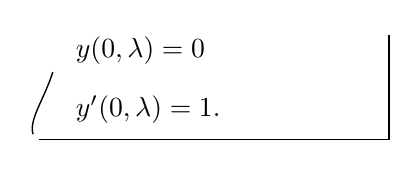
\begin{tikzpicture}[x=1cm,y=1cm]
\node[anchor=west]at(0,.75){$y(0,\lambda)=0$};
\node[anchor=west]at(0,0){$y'(0,\lambda)=1.$};
\draw[line width=.55pt](-.35,-.38)--(4.10,-.38)--(4.10,.95);
\draw[line width=.50pt](-.17,.48)..controls(-.27,.15)and(-.48,-.13)..(-.42,-.31);
\end{tikzpicture}\end{center}
Оно аналит. по $\lambda$.
\SourceFigure{GELFAND-P000111}{normalization-bracket}{Две строки $y(0,\lambda)=0$, $y'(0,\lambda)=1.$. Под ними горизонтальная черта переходит справа в вертикальную вверх. Слева от второй строки отдельный короткий изогнутый штрих, не соединённый с нижней чертой.}
\end{GelfandAdjacentEvidence}
\begin{GelfandAdjacentEvidence}{GELFAND-P000111}{11}

Соб. знач. — когда
$ay'(\pi,\lambda)+by(\pi,\lambda)=0$ имеет ненулев. реш.
Аналит. кривая пересек. почти[?] все [зачёркнуто: неразборчивое слово], прямые,
а по теор. Пикара даже беск. много. (Максимум одно)
\Unclear{GELFAND-P000111}{curve-line-cancellation}{Перед все густо связанное слово: почти / наши; средние штрихи не вполне разделены. После все длинная зачёркнутая запись; действующее прямые следует справа. Следующая строка заканчивается (Максимум одно).}
\end{GelfandAdjacentEvidence}
\begin{GelfandAdjacentEvidence}{GELFAND-P000111}{12}

Как из общ. сообр. получим полноту (кривую в функц. пр-ве) —
это не сделано.
Надо док. теор. в бан. пр-ве — аналит. кривая в бан. пр-ве
(возм., неверно)
[Зачёркнуто: неразборчивая запись.] не прох. через кон. число гиперпл.
\Unclear{GELFAND-P000111}{banach-terminal-cancel}{Перед не прох. отдельная густая отмена с длинным штрихом вниз. Буквы прежней записи не разделены.}
\end{GelfandAdjacentEvidence}
\begin{GelfandAdjacentEvidence}{GELFAND-P000111}{13}

\begin{equation*}ay'(\pi,\lambda)-by(\pi,\lambda)=0.\end{equation*}
\SourceFigure{GELFAND-P000111}{terminal-boundary-minus}{В последней формуле между $ay'$ и $by$ отдельная горизонтальная черта минуса. У $y'$ виден штрих производной; оба аргумента $(\pi,\lambda)$.}
\end{GelfandAdjacentEvidence}



\begin{GelfandAdjacentEvidence}{GELFAND-P000112}{1}
\SourcePage{GELFAND-P000112}{unlabelled}
Точки, в к-рые она попадает, должны быть полн.[?]
\Unclear{GELFAND-P000112}{opening-final-word}{В конце строки полн.[?] / полны; средние штрихи густо слиты, справа отдельная точка. Окончание не установлено.}
\end{GelfandAdjacentEvidence}
\begin{GelfandAdjacentEvidence}{GELFAND-P000112}{2}

Как быть для многих компл. переменных?
Всё это примеры на сл.[?] аналит. пучков (в этих терм. формулир.
и теор. Бореля и Г. Вейля).
\Unclear{GELFAND-P000112}{opening-sheaf-word}{Перед аналит. короткая сл.-подобная запись с густым правым штрихом и точкой. Сокращение не раскрыто.}
\end{GelfandAdjacentEvidence}
\begin{GelfandAdjacentEvidence}{GELFAND-P000112}{3}

Удовлетв. теории, аналог. т-рам Неванлинны, нет.
Распределение нулей $n$ ф-ий $n$ переменных — ?

§ 2. Характеристич. классы (кл. Черна)
\SourceFigure{GELFAND-P000112}{section-heading}{Слева § и отдельное $2$ с точкой. У заголовка не видна нижняя черта. Справа (кл. Черна).}
\end{GelfandAdjacentEvidence}
\begin{GelfandAdjacentEvidence}{GELFAND-P000112}{4}

$X$ — мн-зе, $E$ — вект. рассл., $T=T(X)$ —
[Зачёркнуто: неразборчивая запись.] кас. рассл.
\Unclear{GELFAND-P000112}{tangent-word-cancel}{Перед кас. густо зачёркнут короткий префикс; отдельные прежние буквы не установлены.}
\end{GelfandAdjacentEvidence}
\begin{GelfandAdjacentEvidence}{GELFAND-P000112}{5}

$A^i(X)$ — пучок дифф. форм $i$-го пор.
$\sum A^i(X)=A(X)$ — кольцо.
$d$ — дифф. в $A(X)$, $A(X,E)$ — пучок дифф. форм на $X$ с знач. в $E$.
\begin{equation*}A(X,E)=A(X)\otimes_{A^{0\text{[?]}}(E)}\Gamma(E).\end{equation*}
\Unclear{GELFAND-P000112}{tensor-base}{Под первым тензорным знаком $A^{0\text{[?]}}(E)$: над $A$ округлый знак с маленьким просветом, $0$ / $i$; в скобках E-подобная буква. Под следующим тензорным знаком отдельно $A^0(X)$.}
\end{GelfandAdjacentEvidence}
\begin{GelfandAdjacentEvidence}{GELFAND-P000112}{6}

Обознач.
\begin{equation*}\Gamma(E)\otimes_{A^0(X)}\Gamma(F)\longrightarrow\Gamma(E\otimes F)\end{equation*}
— это умножение обознач. просто точкой.
$E$ — вект. расслоение над $X$.
\underline{Определение.} Связностью на $E$ называется дифф. оператор $D$ на $\Gamma(E)$,
удовл. требованию:
\begin{equation*}
D:\Gamma(E)\longrightarrow\Gamma(T^*\otimes E),\qquad
D(fs)=df\cdot s+f\cdot Ds,\quad s\in\Gamma(E),\ f\in A^0(X).
\end{equation*}
\Unclear{GELFAND-P000112}{definition-title-overwrite}{В подчёркнутом Определение. средние буквы густо переписаны; прежние штрихи отдельно не прочитаны.}
\end{GelfandAdjacentEvidence}
\begin{GelfandAdjacentEvidence}{GELFAND-P000112}{7}

$T^*$ — кокас.[?] (!)
\Unclear{GELFAND-P000112}{cotangent-short-word}{После $T^*$ короткая запись кокас. / конас.; второй согласный густо слит с соседними штрихами. Справа отдельное (!).}
\end{GelfandAdjacentEvidence}
\begin{GelfandAdjacentEvidence}{GELFAND-P000112}{8}

Введём в окр. $U$ мест. координат $\{s_i(x)\}$ — лин. реперы в каждой точке $x$.
\SourceFigure{GELFAND-P000112}{local-frame-word}{Перед фигурной скобкой записано мест. координат; после скобки лин. реперы. Слово координат имеет длинную верхнюю дугу у д и отдельный заключительный штрих.}
\end{GelfandAdjacentEvidence}
\begin{GelfandAdjacentEvidence}{GELFAND-P000112}{9}

\begin{equation*}Ds_i=\sum_{j=1}^n\theta_{ij}s_j.\end{equation*}
$\theta_{ij}$ — матр. связности $\theta(s,D)$.
Её значения — дифф. формы.
\begin{equation*}K(s,D)=d\theta(s,D)-\theta(s,D)\wedge\theta(s,D).\end{equation*}
\SourceFigure{GELFAND-P000112}{curvature-minus}{После первого $\theta(s,D)$ отдельная горизонтальная черта минуса; между следующими матрицами знак $\wedge$.}
\end{GelfandAdjacentEvidence}
\begin{GelfandAdjacentEvidence}{GELFAND-P000112}{10}

Не $0$ т.к. это произв. матриц
\begin{equation*}\sum_l\theta_{il}(s,D)\wedge\theta_{lj}(s,D).\end{equation*}
\SourceFigure{GELFAND-P000112}{curvature-indices}{Под суммой отдельное $l$; у первого $\theta$ нижние $i,l$, у второго $l,j$. У обоих множителей аргументы $(s,D)$.}
\end{GelfandAdjacentEvidence}
\begin{GelfandAdjacentEvidence}{GELFAND-P000112}{11}

Эта внешн. $2$-форма наз. кривизной.
$2$ формы коммут. между собой, поэтому им. смысл $\det$ из форм.
Хар. классы наз.
\begin{equation*}C(E,D\text{[?]})=\operatorname{Det}\left(1+\frac{2\pi}{i}K(s,D)\right).\end{equation*}
\Unclear{GELFAND-P000112}{chern-second-argument}{В $C(E,D\text{[?]})$ второй аргумент бледный, округлый, с густым левым штрихом; $D$ / C-подобная буква.}
\end{GelfandAdjacentEvidence}
\begin{GelfandAdjacentEvidence}{GELFAND-P000112}{12}

\SourceFigure{GELFAND-P000112}{chern-prefactor}{В дроби $2\pi$ над чертой, $i$ под ней; перед дробью плюс, справа $K(s,D)$.}
\end{GelfandAdjacentEvidence}
\begin{GelfandAdjacentEvidence}{GELFAND-P000112}{13}

Это замкнутые $2$-формы.
[Справа:] Формы разных порядков — и набор хар. класс.
\SourceFigure{GELFAND-P000112}{closed-form-degree}{В нижней строке буквально $2$-формы. Отдельная запись в правом поле: Формы разных порядков — и набор хар. класс.}
\end{GelfandAdjacentEvidence}



\begin{GelfandAdjacentEvidence}{GELFAND-P000113}{1}
\SourcePage{GELFAND-P000113}{73}
\begin{flushright}\tikz[baseline=(number.base)]{\node[inner sep=2pt](number){$73$};\draw([xshift=2pt]number.north east)--(number.north west)--(number.south west)--([xshift=2pt]number.south east);}\end{flushright}
Докаж., что $C$ не зав. от выб. базиса и явл. замкн. формой;
на самом деле не зав. и от выб. связности.
\noindent\tikz[baseline=(title.base)]{\node[inner sep=0pt,outer sep=0pt](title){Независимость от выбора базиса.};\draw[decorate,decoration={snake,amplitude=.35mm,segment length=5mm}]([yshift=-2pt]title.south west)--([yshift=-2pt]title.south east);}
\begin{align*}
s'_i&=\sum A_{ij}s_j,\qquad s'=As;\\
Ds'&=dA\cdot s+A\theta(s,D)s,\\
Ds'&=\theta(s',D)s',\\
dA+A\theta(s,D)&=\theta(s',D)A.
\end{align*}
Подставим это в определение $K$.
\begin{center}\tikz[baseline=(eq.base)]{\node[inner sep=2pt](eq){$AK(s,D)=K(s',D)A$};\draw([xshift=-1mm,yshift=2mm]eq.south west)--([xshift=-1mm]eq.south west)--([xshift=1mm]eq.south east)--([xshift=1mm,yshift=2mm]eq.south east);}\end{center}
\begin{equation*}dA\cdot\theta(s,D)+Ad\theta(s,D)=d\theta(s,D)A+\theta(s',D)dA.\end{equation*}
\Unclear{GELFAND-P000113}{differentiated-frame-argument}{В первом $d\theta$ справа аргумент $s$ без отдельного штриха. В следующем $\theta$ аргумент $s'$ со штрихом.}
\end{GelfandAdjacentEvidence}
\begin{GelfandAdjacentEvidence}{GELFAND-P000113}{2}

\SourceFigure{GELFAND-P000113}{differentiated-product-plus}{Справа между $d\theta(s,D)A$ и $\theta(s',D)dA$ отдельный знак плюса с пересекающимися горизонтальным и вертикальным штрихами.}
\end{GelfandAdjacentEvidence}
\begin{GelfandAdjacentEvidence}{GELFAND-P000113}{3}

«$A^{-1}KA^{+1\text{[?]}}$» тот же $\det$.
\Unclear{GELFAND-P000113}{conjugation-exponent}{Над последним $A$ два густых приподнятых штриха, текущая запись $+1$[?]; справа вертикальный штрих сближен с закрывающей кавычкой. Отдельный минус не виден.}
\end{GelfandAdjacentEvidence}
\begin{GelfandAdjacentEvidence}{GELFAND-P000113}{4}


\noindent\tikz[baseline=(title.base)]{\node[inner sep=0pt,outer sep=0pt](title){В. И. Арнольд.};\draw[decorate,decoration={snake,amplitude=.35mm,segment length=5mm}]([yshift=-2pt]title.south west)--([yshift=-2pt]title.south east);}
Прогресс в теории особ. дифф. отображений.
$f:M^m\longrightarrow N^n$ — $2$ многообр.
\Unclear{GELFAND-P000113}{target-letter-overwrite}{В целевом $N^n$ большая буква густо переписана; отдельные прежние штрихи не прочитаны.}
\end{GelfandAdjacentEvidence}
\begin{GelfandAdjacentEvidence}{GELFAND-P000113}{5}

$R^m\longrightarrow R^n$, $0\longrightarrow0$.
Whitney, Thom, Malgrange, B. Morin, Broadman, Mather,
(Haefliger, H. Levin, M. Mors).
\SourceFigure{GELFAND-P000113}{names-spellings}{В латинском списке написаны Broadman, H. Levin и M. Mors; перед Morin B-подобная большая буква.}
\end{GelfandAdjacentEvidence}
\begin{GelfandAdjacentEvidence}{GELFAND-P000113}{6}

Простейш. случай — теор. Морса $n=1$ — крит. точки $df=0$.
$\leftarrow$ для общ. полож. изолир.
Опр. [Зачёркнуто: од…-подобная запись, продолжение неразборчиво.] индексом и сигнатурой.
(лемма Морса) — образец теории.
\Unclear{GELFAND-P000113}{morse-cancel}{После Опр. отменён короткий токен с од…-подобным началом. Середина и конец густо закрыты штрихами.}
\end{GelfandAdjacentEvidence}
\begin{GelfandAdjacentEvidence}{GELFAND-P000113}{7}

Изуч. грубость[?] особенностей (если мало изм., то экв. или нет).
\Unclear{GELFAND-P000113}{depth-word-overwrite}{Начало слова после Изуч. густо переписано. Текущая запись грубость[?], с б-подобной верхней дугой и окончанием ость; прежние штрихи не установлены.}
\end{GelfandAdjacentEvidence}
\begin{GelfandAdjacentEvidence}{GELFAND-P000113}{8}

\begin{center}
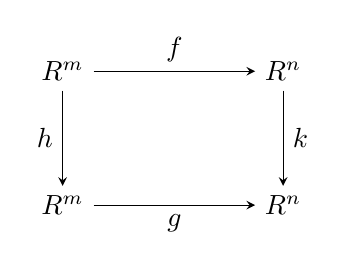
\begin{tikzpicture}[x=28mm,y=17mm,>=stealth]
\node (tl) at (0,1){$R^m$};\node (tr) at (1,1){$R^n$};
\node (bl) at (0,0){$R^m$};\node (br) at (1,0){$R^n$};
\draw[->](tl)--node[above]{$f$}(tr);
\draw[->](bl)--node[below]{$g$}(br);
\draw[->](tl)--node[left]{$h$}(bl);
\draw[->](tr)--node[right]{$k$}(br);
\end{tikzpicture}
\end{center}

$f,g$ экв., если получ. зам. перем.
\SourceFigure{GELFAND-P000113}{coordinate-equivalence-square}{Верхняя и нижняя строки $R^m\to R^n$ с $f$ сверху и $g$ снизу. Вертикальные стрелки направлены вниз: $h$ слева, $k$ справа.}
\end{GelfandAdjacentEvidence}
\begin{GelfandAdjacentEvidence}{GELFAND-P000113}{9}


$d^2f$ без нулей — привод. к квадр. форме.
Для комп.[?] исх. мн. они всюду пл.[?] откр. мн-во.
\Unclear{GELFAND-P000113}{normal-form-density-word}{После Для короткое комп.[?] / норм.; после всюду короткое пл.[?] / на. с точкой. Сокращения не раскрыты. Справа откр. мн-во.}
\end{GelfandAdjacentEvidence}
\begin{GelfandAdjacentEvidence}{GELFAND-P000113}{10}

$R^m\longrightarrow R^1$ решено.
Первый рез. Уитни ($55$ г.) $R^2\longrightarrow R^2$.
Пример особ.
Особые точки — ранг дифф. $=1$ и они $2$-х классов
(складки и сборки). Они структ. уст. ($0$ можно избежать).
\noindent\tikz[baseline=(title.base)]{\node[inner sep=0pt,outer sep=0pt](title){Обычн. точка};\draw[decorate,decoration={snake,amplitude=.35mm,segment length=5mm}]([yshift=-2pt]title.south west)--([yshift=-2pt]title.south east);}
\tikz[baseline=(cancel.base)]{\node[inner sep=0pt,outer sep=0pt](cancel){$(x,y)\longrightarrow(x,y)$};\draw([yshift=2pt]cancel.west)--([yshift=2pt]cancel.east);\draw([yshift=-3pt]cancel.west)--([yshift=-3pt]cancel.east);} $y_1=x_1$, $y_2=x_2$.
\Unclear{GELFAND-P000113}{ordinary-coordinate-cancel}{Запись $(x,y)\longrightarrow(x,y)$ зачёркнута двумя длинными горизонтальными линиями. Справа отдельно $y_1=x_1$, $y_2=x_2$.}
\end{GelfandAdjacentEvidence}
\begin{GelfandAdjacentEvidence}{GELFAND-P000113}{11}

\noindent\tikz[baseline=(title.base)]{\node[inner sep=0pt,outer sep=0pt](title){Точка складки:};\draw[decorate,decoration={snake,amplitude=.35mm,segment length=5mm}]([yshift=-2pt]title.south west)--([yshift=-2pt]title.south east);}
[Зачёркнуто: $(x,y)$[?], другие штрихи не прочитаны.] структ. устойч.
\Unclear{GELFAND-P000113}{fold-coordinate-cancel}{Под заголовком густо зачёркнута $(x,y)$-подобная запись; после нижних косых штрихов отдельные буквы не разделены.}
\end{GelfandAdjacentEvidence}
\begin{GelfandAdjacentEvidence}{GELFAND-P000113}{12}

\begin{equation*}\boxed{\begin{aligned}y_1&=x_1^2,\\y_2&\to x_2.\end{aligned}}\end{equation*}
\SourceFigure{GELFAND-P000113}{fold-normal-form-box}{Две строки в общей рамке. Первая $y_1=x_1^2$. Во второй между $y_2$ и $x_2$ стрелкоподобный знак, горизонтальный штрих с остриём справа.}
\end{GelfandAdjacentEvidence}
\begin{GelfandAdjacentEvidence}{GELFAND-P000113}{13}

\begin{center}
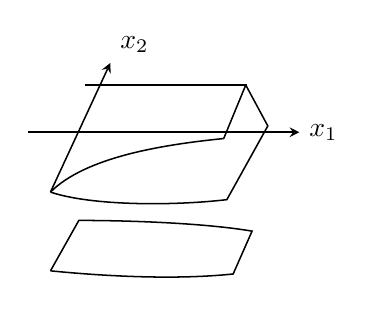
\begin{tikzpicture}[x=8mm,y=8mm,>=stealth,line width=.55pt]
\draw(.55,1.7)--(3.1,1.7)--(2.75,.85);
\draw(0,0)..controls(.65,-.22)and(1.95,-.22)..(2.8,-.12)--(3.45,1.05)--(3.1,1.7);
\draw(0,0)..controls(.55,.55)and(1.75,.75)..(2.75,.85);
\draw[->](-.35,.95)--(3.95,.95)node[right]{$x_1$};
\draw[->](0,0)--(.95,2.05)node[above right]{$x_2$};
\draw(0,-1.25)--(.45,-.45)..controls(1.35,-.45)and(2.5,-.5)..(3.2,-.62)--(2.9,-1.3)..controls(1.95,-1.4)and(.8,-1.33)..(0,-1.25);
\end{tikzpicture}
\end{center}
\SourceFigure{GELFAND-P000113}{fold-sketch}{Две отдельные наклонные полосы. У верхней изогнутый передний край и внутренняя линия; ось $x_1$ направлена вправо, $x_2$ наклонно вверх. Нижняя полоса без подписей.}
\end{GelfandAdjacentEvidence}
\begin{GelfandAdjacentEvidence}{GELFAND-P000113}{14}

\noindent\tikz[baseline=(title.base)]{\node[inner sep=0pt,outer sep=0pt](title){Точка сборки:};\draw[decorate,decoration={snake,amplitude=.35mm,segment length=5mm}]([yshift=-2pt]title.south west)--([yshift=-2pt]title.south east);}
\begin{center}\tikz[baseline=(cusp.base)]{\node[inner sep=2pt](cusp){$\begin{aligned}y_1&\mathrel{\overset{\text{[?]}}{\to}}x_1,\\y_2&=x_2^3-x_1x_2.\end{aligned}$};\draw(cusp.south west)--(cusp.south east);}\end{center}
\Unclear{GELFAND-P000113}{cusp-formula-minus}{У $y_1$ знак с двумя сближенными штрихами, $\to$ / $=$; справа $x_1$. Во второй строке $y_2=x_2^3-x_1x_2$, с отдельным минусом. Под обеими строками длинная прямая черта.}
\end{GelfandAdjacentEvidence}
\begin{GelfandAdjacentEvidence}{GELFAND-P000113}{15}

\begin{center}\begin{tikzpicture}[x=1mm,y=1mm]
\node[anchor=north west,inner sep=0pt,align=left,text width=116mm] at(2,-2){$z^2$ особ. неустойч. при деф. расщ.\\\hspace*{47mm}на $3$ точки сборки.};
\draw(120,0)--(0,0)..controls(-2,0)and(-2,-10)..(0,-10)--(45,-10)--(43,-15)--(120,-15);
\end{tikzpicture}\end{center}
\SourceFigure{GELFAND-P000113}{squared-map-callout}{Справа запись в рамке, открытой с правого края; в нижнем контуре ступенька. Текст начинается с $z^2$, в следующей строке на $3$ точки сборки.}
\end{GelfandAdjacentEvidence}
\begin{GelfandAdjacentEvidence}{GELFAND-P000113}{16}

Теор. Уитни: любое [Зачёркнуто: неразборчивая запись.] отобр. аппрокс. такими.
\Unclear{GELFAND-P000113}{whitney-cancel}{Между любое и отобр. короткая густая отмена. Прежние буквы не установлены.}
\end{GelfandAdjacentEvidence}

Точки $3$-го типа изолир., $2$-го типа в $M^m$ без особ.
$1$-мерн. мн-же, в $N$ у него особ.


\begin{GelfandAdjacentEvidence}{GELFAND-P000114}{1}
\SourcePage{GELFAND-P000114}{unlabelled}
\noindent\tikz[baseline=(title.base)]{\node[inner sep=0pt,outer sep=0pt](title){Сборка.};\draw[decorate,decoration={snake,amplitude=.35mm,segment length=5mm}]([yshift=-2pt]title.south west)--([yshift=-2pt]title.south east);} Якобиан
\begin{equation*}\left|\begin{matrix}1&0\\-x_2&3x_2^2-x_1\end{matrix}\right|.\end{equation*}
$3x_2^2-x_1=0$ парабола.
В $0$ складка, но в целом сложнее.
\SourceFigure{GELFAND-P000114}{origin-fold-wording}{Справа отдельные строки В $0$ складка, но / в целом сложнее.}
\end{GelfandAdjacentEvidence}
\begin{GelfandAdjacentEvidence}{GELFAND-P000114}{2}

\begin{center}\begin{tikzpicture}[x=9mm,y=9mm,>=stealth,line width=.55pt]
\draw[->](-1.2,0)--(1.9,0)node[right]{$x_1$};
\draw[->](0,-1.35)--(0,1.65)node[above right]{$x_2$};
\draw(1.6,1.05)..controls(.5,.85)and(0,.55)..(0,0)..controls(0,-.6)and(.6,-1.05)..(1.55,-1.08);
\draw[->](4.6,0)--(7.4,0)node[right]{$y_1$};
\draw[->](6,-1.4)--(6,1.65)node[above left]{$y_2$};
\draw(6,0)..controls(6.45,0)and(6.95,.7)..(7.15,1.45);
\draw(6,0)..controls(6.45,0)and(6.9,-.6)..(7.1,-1.3);
\end{tikzpicture}\end{center}
\SourceFigure{GELFAND-P000114}{critical-curve-images}{Слева парабола с вершиной в начале координат, $x_1$ вправо, $x_2$ вверх. Справа две ветви с общим остриём, направленные вправо; $y_1$ вправо, $y_2$ вверх.}
\end{GelfandAdjacentEvidence}
\begin{GelfandAdjacentEvidence}{GELFAND-P000114}{3}

Куда перех. парабола?
[Зачёркнуто: $y_2=\text{[?]}y_1^{3/2}$.]
\Unclear{GELFAND-P000114}{cusp-equation-cancel}{В отменённой записи видны $y_2$, знак равенства, $y_1^{3/2}$. Коэффициент и промежуточные штрихи густо закрыты.}
\end{GelfandAdjacentEvidence}
\begin{GelfandAdjacentEvidence}{GELFAND-P000114}{4}

$y_2=-Cy_1^{3/2}$.
\begin{center}\tikz[baseline=(eq.base)]{\node[inner sep=2pt](eq){$y_2^2=-y_1^3$};\draw([yshift=3mm]eq.south west)--(eq.south west)--(eq.south east)--([yshift=3mm]eq.south east);}\end{center}
$y_1>0$.
\SourceFigure{GELFAND-P000114}{negative-cusp-square}{В угловой рамке $y_2^2=-y_1^3$, с отдельным минусом. Ниже и левее отдельная запись $y_1>0$.}
\end{GelfandAdjacentEvidence}
\begin{GelfandAdjacentEvidence}{GELFAND-P000114}{5}

Отобр. не есть складка на всей параболе.
Вне точки $0$ складка.
Рассм. прямые, паралл. оси $x_2$.
$x_1=\operatorname{const}\Rightarrow y_1=\operatorname{const}$.
$y_2=x_2^3-Cx_2$.
\SourceFigure{GELFAND-P000114}{cubic-parameter-line}{В строке $x_1=\operatorname{const}$ стрелка к $y_1=\operatorname{const}$. Ниже $y_2=x_2^3-Cx_2$, с большой C-подобной буквой перед $x_2$.}
\end{GelfandAdjacentEvidence}
\begin{GelfandAdjacentEvidence}{GELFAND-P000114}{6}

\begin{center}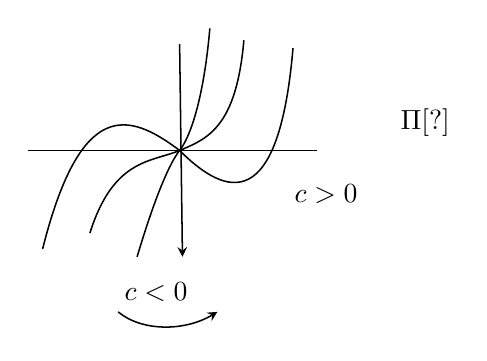
\begin{tikzpicture}[x=12mm,y=10mm,>=stealth,line width=.55pt]
\draw(-1.6,0)--(1.45,0);
\draw[->](0,1.35)--(.03,-1.35);
\draw(-1.45,-1.25)..controls(-1.05,.65)and(-.55,.5)..(0,0)..controls(.5,-.6)and(1.05,-.8)..(1.2,1.3);
\draw(-.95,-1.05)..controls(-.7,-.1)and(-.3,-.15)..(0,0)..controls(.3,.15)and(.6,.3)..(.68,1.4);
\draw(-.45,-1.35)..controls(-.25,-.55)and(-.1,-.15)..(0,0)..controls(.1,.15)and(.25,.6)..(.32,1.55);
\node at(1.55,-.55){$c>0$};\node at(-.25,-1.8){$c<0$};
\draw[->](-.65,-2.05)..controls(-.4,-2.3)and(.05,-2.3)..(.4,-2.05);
\node at(2.6,.35){$\Pi\text{[?]}$};
\end{tikzpicture}\end{center}
\Unclear{GELFAND-P000114}{cubic-family-sketch}{Несколько кривых проходят через общее пересечение осей. Справа у кривой с поворотами $c>0$; снизу $c<0$ и изогнутая стрелка. Справа отдельная П-/ $\Pi$-подобная метка, значение не установлено.}
\end{GelfandAdjacentEvidence}
\begin{GelfandAdjacentEvidence}{GELFAND-P000114}{7}

$c<0$ прямые отобр. изом.[?] $c>0$.
\Unclear{GELFAND-P000114}{cubic-map-word}{После отобр. короткое изом.[?] / монот.-подобное слово с густо слитыми средними штрихами. Сокращение не раскрыто.}
\end{GelfandAdjacentEvidence}
\begin{GelfandAdjacentEvidence}{GELFAND-P000114}{8}

\begin{center}\begin{tikzpicture}[x=9mm,y=9mm,>=stealth,line width=.55pt]
\draw[->](-1.5,0)--(1.8,0);\draw[->](0,-1.2)--(0,1.65);
\draw(1.2,1.25)..controls(.4,1.1)and(0,.55)..(0,0)..controls(0,-.55)and(.45,-1)..(1.25,-1.02);
\draw(-.65,-1.05)--(-.65,1.4);\draw(.8,-1.4)--(.8,1.65);
\node at(3.15,.45){$c>0$};
\draw(4.8,0)--(7.8,0);\draw(5.65,-1.15)--(5.65,1.15);
\draw(5.65,0)..controls(6.1,0)and(6.65,.55)..(7.15,1.1);
\draw(5.65,0)..controls(6.1,0)and(6.6,-.45)..(7.15,-1.3);
\draw(6.5,-1.45)--(6.5,1.5);\draw(6.9,-1.2)--(6.9,.85);
\draw(6.55,.6)..controls(6.35,.3)and(6.45,-.1)..(6.3,-.4);
\end{tikzpicture}\end{center}
\SourceFigure{GELFAND-P000114}{vertical-line-sketches}{Слева парабола, оси и две отдельные вертикали. Справа двуветвенная заострённая кривая с несколькими вертикальными штрихами и короткой изогнутой внутренней линией. Между схемами $c>0$.}
\end{GelfandAdjacentEvidence}
\begin{GelfandAdjacentEvidence}{GELFAND-P000114}{9}

Сборка есть на всех лучесных[?] бранах[?].
\Unclear{GELFAND-P000114}{ray-wording}{В первом спорном слове вертикальный штрих рисунка пересекает середину: лучевых / лучесных. Во втором начальные штрихи б-/г-подобны: бранах / гранях. Полное чтение не установлено.}
\end{GelfandAdjacentEvidence}
\begin{GelfandAdjacentEvidence}{GELFAND-P000114}{10}

\underline{Задача.}
[Зачёркнуто: $z^2$[?] и неразборчивые штрихи.]
$z\longrightarrow z^2+\varepsilon\overline z$ — общ. полож.
$\varepsilon=0$ особ. в $0$; при $\varepsilon\ne0$ она смещается,
будут складки и сборки. И только это устойчиво.
\Unclear{GELFAND-P000114}{square-map-cancel}{После Задача. отменён z-подобный знак с верхним $2$; правая часть записи закрыта длинными штрихами.}
\end{GelfandAdjacentEvidence}
\begin{GelfandAdjacentEvidence}{GELFAND-P000114}{11}

\noindent\tikz[baseline=(title.base)]{\node[inner sep=0pt,outer sep=0pt](title){Научное опред. сборки.};\draw[decorate,decoration={snake,amplitude=.35mm,segment length=5mm}]([yshift=-2pt]title.south west)--([yshift=-2pt]title.south east);}
Одна из изв. сист. инв.
Ранг $=r\text{[?]}$ — многообр. $\Sigma_r$.
\Unclear{GELFAND-P000114}{rank-letter}{После знака равенства буква густо переписана; текущая запись $r$[?], прежние округлые штрихи отдельно не прочитаны. Ниже сходные знаки у $\Sigma_r$ и в цепочке $r_1,r_2$.}
\end{GelfandAdjacentEvidence}
\begin{GelfandAdjacentEvidence}{GELFAND-P000114}{12}

$M^m$ разбив. на мн-же.
\tikz[baseline=(cancel.base)]{\node[inner sep=0pt](cancel){Коразм.};\draw([yshift=2pt]cancel.west)--([yshift=2pt]cancel.east);\draw([yshift=-2pt]cancel.west)--([yshift=-2pt]cancel.east);}

\begin{center}\begin{tikzpicture}[x=1mm,y=1mm,baseline=(codim.base)]
\node[anchor=base west,inner sep=0pt](codim) at(0,0){Коразм.};
\node[anchor=base west,inner sep=0pt] at(25,0){особ.};
\node[anchor=base west,inner sep=0pt] at(43,0){$=$};
\node[anchor=base west,inner sep=0pt](prod) at(51,0){произв. корангов};
\node[anchor=base west,inner sep=0pt] at(105,0){$(m-r)(n-r)$};
\node[inner sep=0pt] at(29,-10){мн-же};
\draw(17,-8)..controls(17,-5)and(18,-5)..(21,-5)..controls(25,-5)and(28,-4)..(29,-2)..controls(30,-4)and(33,-4)..(37,-4)..controls(41,-4)and(41,-6)..(42,-8);
\draw(0,-8)--(0,-14)--(45,-14)--(45,-6);
\draw[decorate,decoration={snake,amplitude=.35mm,segment length=5mm}]([yshift=-2pt]prod.south west)--([yshift=-2pt]prod.south east);
\end{tikzpicture}\end{center}

(Это вопр. о независ. минорах прямоуг. матр. ранга $r$.)
\Unclear{GELFAND-P000114}{codimension-cancel}{Первое Коразм. зачёркнуто длинными горизонтальными линиями. Ниже отдельное повторение Коразм. особ.}
\end{GelfandAdjacentEvidence}
\begin{GelfandAdjacentEvidence}{GELFAND-P000114}{13}

\SourceFigure{GELFAND-P000114}{rank-codimension-brackets}{Под особ. фигурная скобка с остриём вверх и подпись мн-же; ниже длинная угловая рамка. Произв. корангов подчёркнуто волнистой линией; справа $(m-r)(n-r)$.}
\end{GelfandAdjacentEvidence}
\begin{GelfandAdjacentEvidence}{GELFAND-P000114}{14}


$\Sigma_r$ — гладкие мн-же в $R^m$; рассм. наше отобр. на самих
мн-жах (парабола). Ранг на этих мн-жах.
$\Sigma_{r_1,r_2}$, $r_2<r_1$ — подмн-же — уровни ранга.
$\Sigma_{r_1,r_2,r_3}$.
Каждой [Зачёркнуто: неразборчивое слово.] особ. соот. набор чисел $r_1,r_2,r_3$.
\Unclear{GELFAND-P000114}{invariant-cancel}{После Каждой отменено длинное слово, особенности-подобное. Верхние и нижние горизонтальные штрихи закрывают большую часть букв.}
\end{GelfandAdjacentEvidence}

Инвариант особенности $r_1\ge r_2\ge\cdots\ge0$.


\begin{GelfandAdjacentEvidence}{GELFAND-P000115}{1}
\SourcePage{GELFAND-P000115}{74}
Особ. Уитни: \tikz[baseline=(sigma.base)]{\node[inner sep=0pt](sigma){$\Sigma_0$};\node[anchor=north,inner sep=0pt,font=\small] at([yshift=-1pt]sigma.south){обычн.};}.
Первый индекс — коранг.
Сборка: $\Sigma_{10}$. Доказано, что это мн-же.
\SourceFigure{GELFAND-P000115}{sigma-examples}{У Уитни $\Sigma_0$, под ним обычн.; у сборки $\Sigma_{10}$. Справа Первый индекс — коранг.}
\end{GelfandAdjacentEvidence}
\begin{GelfandAdjacentEvidence}{GELFAND-P000115}{2}

[Зачёркнуто: Д…]

Для разб. в пр-ве отрезков рядов Тейлора. (Бродман) —
старый наивн. подход.
\Unclear{GELFAND-P000115}{top-cancel}{Перед для разб. короткая отменённая запись; Д-подобное начало видно, остальные буквы закрыты штрихами.}
\end{GelfandAdjacentEvidence}
\begin{GelfandAdjacentEvidence}{GELFAND-P000115}{3}


Изв., что $\Sigma$ не явл. полной классифик.
(Есть пример $R^9\longrightarrow R^9$.)
\underline{Общая теория.} Рассм. пр-во рядов Тейлора.
($3$ класса — $C^\infty$, анал., форм. степ. ряды.)
[Справа:] $R^m\longrightarrow R^n$; $C^\infty$ есть ряды Тейлора.
\begin{equation*}y=\sum_{k\mathrel{\overset{\text{[?]}}{\ge}}0}a_kx^k,\qquad a_k\text{ — вектор},\quad k=(k_1,\ldots,k_m).\end{equation*}
\Unclear{GELFAND-P000115}{multiindex-series}{Под суммой $k\ge0$[?] / $k>0$; мелкие штрихи знака слиты. Справа $a_k$ — вектор, $k=(k_1,\ldots,k_m)$.}
\end{GelfandAdjacentEvidence}
\begin{GelfandAdjacentEvidence}{GELFAND-P000115}{4}

Лок. теории.
$C^\infty$ — самый трудный, анал. — самый интер., форм. ряды —
самая прост.
Отобр. экв. — если сущ. замена.
Возник. разб. на куски — стратификация. Изуч. этого разбиения.
\begin{center}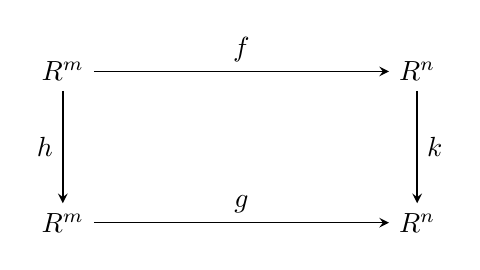
\begin{tikzpicture}[x=15mm,y=12mm,>=stealth,line width=.55pt]
\node(A)at(0,0){$R^m$};\node(B)at(3,0){$R^n$};
\node(C)at(0,-1.6){$R^m$};\node(D)at(3,-1.6){$R^n$};
\draw[->](A)--node[above]{$f$}(B);
\draw[->](C)--node[above]{$g$}(D);
\draw[->](A)--node[left]{$h$}(C);
\draw[->](B)--node[right]{$k$}(D);
\end{tikzpicture}\end{center}

$h,k$ — форм. дифф. ($1$-е члены с якоб. $\ne0$).
\SourceFigure{GELFAND-P000115}{formal-equivalence-square}{Два ряда $R^m\to R^n$: сверху $f$, снизу $g$; вертикальные стрелки вниз, слева $h$, справа $k$.}
\end{GelfandAdjacentEvidence}
\begin{GelfandAdjacentEvidence}{GELFAND-P000115}{5}


Есть пример ($>9$) с беск. числом инвар.
\noindent\tikz[baseline=(title.base)]{\node[inner sep=0pt](title){Том};\draw[decorate,decoration={snake,amplitude=.35mm,segment length=5mm}]([yshift=-2pt]title.south west)--([yshift=-2pt]title.south east);\draw[->]([xshift=-8mm,yshift=6mm]title.west)--([xshift=-6mm,yshift=-1mm]title.west); } доказал, что в пр-ве степ. рядов выдел. часть коразм. беск.,
что ост. грубые в топ. смысле.
\Unclear{GELFAND-P000115}{headings-and-arrow}{Общая теория. подчёркнуто прямой линией, средние буквы переписаны. Том подчёркнуто волнистой линией; слева короткая стрелка вниз. Более ранние штрихи имени отдельно не прочитаны.}
\end{GelfandAdjacentEvidence}
\begin{GelfandAdjacentEvidence}{GELFAND-P000115}{6}

(Инв. Тома в $R^9$ есть инв. гладких, но не непр.[?])
\Unclear{GELFAND-P000115}{tom-invariant-abbreviation}{Последнее сокращение непр. / нерп.; слитые средние штрихи не дают однозначного порядка букв.}
\end{GelfandAdjacentEvidence}
\begin{GelfandAdjacentEvidence}{GELFAND-P000115}{7}

(Том не хочет публик. док-во, он заним. биологией.
Док-во рассказ., целый год, но его никто не понял:
Malgrange, Cartan, Арнольд и др.)
$\bigcup X_\gamma+X_\infty$, $X_\gamma$ грубые в топ. смысле особ.
\SourceFigure{GELFAND-P000115}{strata-union-sign}{Перед $X_\gamma$ большой знак объединения без нижнего индекса; между $X_\gamma$ и $X_\infty$ отдельный плюс.}
\end{GelfandAdjacentEvidence}
\begin{GelfandAdjacentEvidence}{GELFAND-P000115}{8}

При нек-рых разм. анал. трудностей Тома не возник.
(Особ. грубые дифф.)
Как будто бы реш. зад., где есть
[Зачёркнуто: неразборчивое слово.]
классифиц. (в малых разм.)
\Unclear{GELFAND-P000115}{classification-cancel}{Между есть и классифиц. длинная отменённая запись, закрытая несколькими горизонтальными штрихами.}
\end{GelfandAdjacentEvidence}
\begin{GelfandAdjacentEvidence}{GELFAND-P000115}{9}

Сущ. $\Sigma$, явл. дифф. грубыми $\Sigma_{1,\ldots,1,0}$.
Не все $\Sigma$ дифф. грубыми.
Ещё один рез. Mother. (Учен. Милнора.)
\SourceFigure{GELFAND-P000115}{mather-source-spelling}{В имени округлое $o$: Mother. В нижнем повторении Mother′а.}
\end{GelfandAdjacentEvidence}
\begin{GelfandAdjacentEvidence}{GELFAND-P000115}{10}

$\delta y=\varphi(x)$.
$h(x)$ — вар. в $X$ — вект. поле.
\begin{center}\begin{tikzpicture}[x=12mm,y=12mm,>=stealth,line width=.55pt]
\draw(-1.2,0)--(2.15,0);\draw(0,-.7)--(0,1.8);
\draw(.25,.85)..controls(.65,1.55)and(1.15,1.8)..(1.7,1.45);
\draw(.25,.45)..controls(.6,1.25)and(1.15,1.4)..(1.65,.9);
\node[right]at(1.65,.9){$f(x)$};
\draw[->](.65,-.3)--(1.65,-.3)node[below]{$h(x)$};
\draw[->](-.75,.4)--(-.75,1.35)node[left]{$k(y)$};
\end{tikzpicture}\end{center}
\SourceFigure{GELFAND-P000115}{variation-sketch}{Пересекающиеся оси и две близкие дуги над горизонталью, у нижней $f(x)$. Отдельная горизонтальная стрелка вправо ниже оси подписана $h(x)$, вертикальная вверх слева — $k(y)$.}
\end{GelfandAdjacentEvidence}
\begin{GelfandAdjacentEvidence}{GELFAND-P000115}{11}

Замена пер. — ф-я изм. на $f'(x)h(x)+k(y)$.
В $1$-м приб. надо решить ур-е
\begin{equation*}\varphi(x)=f'(x)h(x)+k(y).\end{equation*}
\Unclear{GELFAND-P000115}{linear-k-overwrite}{В первой формуле $k(y)$ густо переписано; ниже в отдельном уравнении чистое $k(y)$. Прежние штрихи первой буквы не прочитаны.}
\end{GelfandAdjacentEvidence}
\begin{GelfandAdjacentEvidence}{GELFAND-P000115}{12}

Соотв. теор. сост. в том, что для грубости необх. и дост.,
чтобы решалась соотв. лин. задача. ($\forall\varphi(x)$)
(сек. верхних.[?] пучки[?])
\Unclear{GELFAND-P000115}{sheaf-parenthetical}{Начало сек.; следующее слово верхних.[?] / вер…них.-подобное, полное чтение не установлено. Последнее пучки / пучка.}
\end{GelfandAdjacentEvidence}
\begin{GelfandAdjacentEvidence}{GELFAND-P000115}{13}

(Это $1$-я теор. Mother′а. Более того, дост. для $\varphi(x)$,
зад. многом. степени, равной разм. $\ell\text{[?]}$.)
\Unclear{GELFAND-P000115}{jet-power-overwrite}{После разм. густо переписанный знак, $\ell$- / $N$-подобный; прежние штрихи закрыты.}
\end{GelfandAdjacentEvidence}

Но док-во неверно.
Совр. техника (нелин. ф-и в $C^\infty$-пр-вах).
Найдены все разм., для к-рых всё хорошо.
$R^2\longrightarrow R^2,R^3$ (Уитни); в $R^4$ неизв.,
в $R^5$ уже изв. (уже нет особ. никаких).
Погружение (иммерсия).
При $m=n$ до $8$ все отобр. грубые (аппрокс.).


\begin{GelfandAdjacentEvidence}{GELFAND-P000116}{1}
\SourcePage{GELFAND-P000116}{unlabelled}
Том — континуальный инвариант (грубый).
Он не топ. — он инв. гладких отобр.
При непр. деф. можно их продеф.
29/\underline{XI}. \underline{Ещё} \underline{раз} \underline{о[?]} \underline{хар.} \underline{классах.}
[Зачёркнуто: неразборчивое слово.]

(И. М. Гельфанд.)
\Unclear{GELFAND-P000116}{heading-cancel}{После классах. длинная густо отменённая запись; буквы закрыты горизонтальными штрихами.}
\end{GelfandAdjacentEvidence}
\begin{GelfandAdjacentEvidence}{GELFAND-P000116}{2}


\Unclear{GELFAND-P000116}{heading-and-underlines}{Перед хар. округлая густо переписанная буква о[?], с отдельным прямым подчёркиванием. Части заголовка подчёркнуты отдельно. Красивое соображение. и Классиф.: ниже имеют волнистые подчёркивания.}
\end{GelfandAdjacentEvidence}
\begin{GelfandAdjacentEvidence}{GELFAND-P000116}{3}

Рассм. $E$ над $X$, связность $D:\Gamma(E)\to\Gamma(T^*\otimes E)$.
\tikz[baseline=(f.base)]{\node[inner sep=0pt](f){$f$};\node[anchor=north,inner sep=0pt,font=\small](label)at([yshift=-3mm]f.south){ф-я};\draw(f.south)--(label.north);} $\in A^0$, $s\in\Gamma(E)$ $\Rightarrow$
$D(fs)=f\cdot Ds+df\cdot s$.
[Справа:] (Здесь $T$ — кас.[?] рассл.)
\Unclear{GELFAND-P000116}{tangent-abbreviation-cancel}{Перед и в начале кас. густое исправление; прежние штрихи отдельно не прочитаны.}
\end{GelfandAdjacentEvidence}
\begin{GelfandAdjacentEvidence}{GELFAND-P000116}{4}

[На поле:] \tikz[baseline=(two.base)]{\node[draw,circle,inner sep=1pt](two){$2$};}
Точн. — тенз. пр. в $A\otimes_{A^0}\Gamma(E)$.
\SourceFigure{GELFAND-P000116}{tensor-product-and-annotations}{Под $f$ подпись ф-я, соединённая с буквой коротким штрихом. В тензорном произведении под знаком $\otimes$ стоит $A^0$. На правом поле обведена $2$.}
\end{GelfandAdjacentEvidence}
\begin{GelfandAdjacentEvidence}{GELFAND-P000116}{5}

Подвижн. репер Картана (локально): $s_i$ $(i=1,\ldots,n)$,
$n$ — разм.[?] слоя.

Лин. независ. $\forall$ точке.
\Unclear{GELFAND-P000116}{rank-word-overwrite}{В $n$ — разм. слоя слово разм. густо переписано; предшествующие буквы закрыты.}
\end{GelfandAdjacentEvidence}
\begin{GelfandAdjacentEvidence}{GELFAND-P000116}{6}


$D(s_i)=\sum\theta_{ij}s_j$, коэфф. из $A^1$ (формы).
$\|\theta_{ij}\|$ наз. матрицей связности (у Картана — $\omega$).
\SourceFigure{GELFAND-P000116}{frame-section-symbols}{У сечений повторяется $s$-подобная буква: $s\in\Gamma(E)$, $s_i$, $s_j$; ниже $s=(s_1,\ldots,s_n)$. Начальная $D$ в $D(fs)$ переписана.}
\end{GelfandAdjacentEvidence}
\begin{GelfandAdjacentEvidence}{GELFAND-P000116}{7}

\begin{equation*}
\|K_{ij}\|=K(s,D)=d\theta(s,D)-\theta(s,D)\wedge\theta(s,D),
\qquad s=(s_1,\ldots,s_n).
\end{equation*}
(Это матрица.) (Произв. матриц, но пр. внешнее.)
Форма
\begin{equation*}C(E,D)=\det\left|I+\frac{i}{2\pi}K(s,D)\right|.\end{equation*}
\SourceFigure{GELFAND-P000116}{chern-factor-reversal}{В определителе перед $K(s,D)$ дробь с $i$ в числителе и $2\pi$ в знаменателе.}
\end{GelfandAdjacentEvidence}
\begin{GelfandAdjacentEvidence}{GELFAND-P000116}{8}

Элементы — формы чётного пор., они коммут. и можно брать $\det$.
$\sum$ форм разного пор. Они и есть хар. классы,
связ. с данным рассл. Это не зав. от выбора связности.
[Идея док-ва по Гельфанду: замкнутость и это док., $\theta\text{[?]}$ замен.

Форма уже не зав. от связности, $\int$ можно выраз. через
$\int$ по границе. Вариация связности внутри не влияет.]
\Unclear{GELFAND-P000116}{proof-theta-overwrite}{Перед замен. густой $\theta$- / параграф-подобный знак, с округлым верхним и плотным нижним штрихом.}
\end{GelfandAdjacentEvidence}
\begin{GelfandAdjacentEvidence}{GELFAND-P000116}{9}


От выб. репера не зависит.
Тождество Бианки:
\begin{equation*}dK(s,D)=-[K(s,D),\theta(s,D)].\end{equation*}
(Производная тенз. кривизны.)
\SourceFigure{GELFAND-P000116}{curvature-and-bianchi}{В формуле кривизны минус перед $\theta\wedge\theta$. В тождестве Бианки минус перед коммутатором; порядок внутри скобок $K(s,D),\theta(s,D)$.}
\end{GelfandAdjacentEvidence}
\begin{GelfandAdjacentEvidence}{GELFAND-P000116}{10}

\noindent\tikz[baseline=(title.base)]{\node[inner sep=0pt,outer sep=0pt](title){Красивое соображение.};\draw[decorate,decoration={snake,amplitude=.35mm,segment length=5mm}]([yshift=-2pt]title.south west)--([yshift=-2pt]title.south east);}
$g_{\alpha\beta}(x)$ — рим. метрика, будем брать все послед.
производные $g_{\alpha\beta}(x)$ и составл. из них тензоры.
Как найти все тензоры, к-рые можно составлять из $g_{\alpha\beta}(x)$?
\noindent\tikz[baseline=(title.base)]{\node[inner sep=0pt,outer sep=0pt](title){Классиф.:};\draw[decorate,decoration={snake,amplitude=.35mm,segment length=5mm}]([yshift=-2pt]title.south west)--([yshift=-2pt]title.south east);} они есть ф-и от тензора кривизны и всех ковар.
произв. тенз. кривизны (любой пор.) (алгебр. выраж. от них).
Но какие алгебр. соотн.? (Между первыми ковар. пр. — тожд. Бианки.)
Ввод. норм. коорд. (по[?] геодезич.) мр.[?] рассл.
\Unclear{GELFAND-P000116}{normal-coordinate-wording}{В начале скобок короткое по[?]-подобное слово. После скобок мр.[?] / метр.-подобное сокращение перед рассл.; полное чтение не установлено.}
\end{GelfandAdjacentEvidence}
\begin{GelfandAdjacentEvidence}{GELFAND-P000116}{11}

\begin{equation*}\begin{aligned}
g_{\alpha\beta}(x)&=g_{\alpha\beta}(0)+g_{\alpha\beta,\delta\delta}x^\delta x^\delta\\
&\quad+g_{\alpha\beta,\delta\delta\varepsilon}\text{[?]}x^\delta x^\delta x^\varepsilon.
\end{aligned}\end{equation*}
\Unclear{GELFAND-P000116}{normal-metric-indices}{Во втором члене две $\delta$-подобные буквы в нижних индексах и при обоих $x$. В третьем нижние индексы $\delta\delta\varepsilon$[?] / $\gamma\delta\varepsilon$, средняя буква переписана; верхние индексы также $\delta$- / $\gamma$-подобны, последний $\varepsilon$.}
\end{GelfandAdjacentEvidence}

В норм. сист. все они тензоры.
Эта сист. тензоров и здесь алг. соотн. проще.


\begin{GelfandAdjacentEvidence}{GELFAND-P000117}{1}
\SourcePage{GELFAND-P000117}{75}
\underline{В. И. Арнольд.} Грубое течение.
$\dot x=f(x,C)$; $g^t$ — группа диффеом.
Есть химич. и биологич. модели (Том).
$x$ \tikz[x=1mm,y=1mm,baseline=-.3mm]{\draw(0,0)--(3,0)--(1.5,2.7)--cycle;\fill(1.5,.9)circle(.25);} суммы веществ, $c$ — парам.
\SourceFigure{GELFAND-P000117}{flow-definition-marks}{Между $x$ и суммы веществ треугольник с точкой внутри. В правой подписи параметр обозначен малым $c$, в уравнении большим $C$.}
\end{GelfandAdjacentEvidence}
\begin{GelfandAdjacentEvidence}{GELFAND-P000117}{2}

Рассматр. одно (грубое).
Число когрубости[?] вводится.
\begin{center}\begin{tikzpicture}[x=13mm,y=11mm,>=stealth,line width=.55pt]
\node(A)at(0,0){$X$};\node(B)at(2,0){$X$};\node(C)at(0,-1.5){$X$};\node(D)at(2,-1.5){$X$};
\draw[->](A)--node[above]{$g^t\text{[?]}$}(B);\draw[->](C)--node[above]{$h\text{[?]}$}(D);
\draw[->](A)--(C);\draw[->](B)--(D);
\end{tikzpicture}\end{center}
\Unclear{GELFAND-P000117}{flow-conjugacy-square}{Четыре $X$; над верхней горизонтальной стрелкой переписанное $g^t$[?], над нижней $h$-подобная буква. Горизонтали вправо, вертикали вниз, у вертикалей подписей нет.}
\end{GelfandAdjacentEvidence}
\begin{GelfandAdjacentEvidence}{GELFAND-P000117}{3}

Грубые, если $\forall$ близкого $h$ сущ. возмущ. $X$.
Нельзя рассм. одни грубые (при измен. пар. может прох. негрубые пар.).
$(x,C)$ — точка когрубости[?] $1$, если для близких знач. пар.
груб. и т.д.
Как отобр. $X\times C\longrightarrow X\times C$ грубое.
(Сколько чл. ряд. Тейл. нужно взять.)
Центр — беск. степ. негрубости.
\begin{center}\tikz[x=1mm,y=1mm]{\draw(0,0)circle(5);\draw(0,0)circle(3.4);\draw(0,0)circle(1.5);}\end{center}
\SourceFigure{GELFAND-P000117}{center-circles}{Рядом с записью о центре три вложенные замкнутые округлые линии. Подписей у них нет.}
\end{GelfandAdjacentEvidence}
\begin{GelfandAdjacentEvidence}{GELFAND-P000117}{4}

Теор. Тома о ростках рядов Тейлора
$\vartheta=\vartheta^\infty+\bigcup_\gamma\vartheta^\gamma$.

[Под формулой:] \underline{\underline{коразм. $\infty$}}
\Unclear{GELFAND-P000117}{jet-strata-symbol}{Повторяющаяся буква $\vartheta$[?] / $\theta$ / $O$-подобна, с большой верхней петлёй; верхние индексы $\infty$ и $\gamma$-подобны.}
\end{GelfandAdjacentEvidence}
\begin{GelfandAdjacentEvidence}{GELFAND-P000117}{5}


\SourceFigure{GELFAND-P000117}{jet-codimension-annotation}{Под формулой отдельная надпись коразм. $\infty$, подчёркнутая двумя линиями.}
\end{GelfandAdjacentEvidence}
\begin{GelfandAdjacentEvidence}{GELFAND-P000117}{6}

В $\vartheta^\gamma$ откр. подмн. кон. негруб.[?]
В $\vartheta^\gamma$ особ. описыв. конеч. числом парам., внутри
[Зачёркнуто: неразборчивый короткий токен.]

$\vartheta^\gamma$ все диффеом. (Тр-ие для дифф. ур-й.)
\Unclear{GELFAND-P000117}{inside-stratum-cancel}{После внутри короткая густая отмена; отдельно слева ещё короткий горизонтальный штрих.}
\end{GelfandAdjacentEvidence}
\begin{GelfandAdjacentEvidence}{GELFAND-P000117}{7}


В $\vartheta^\infty$ полный хаос (но они конеч. коразм.[?]).
Все $1$-параметрич. в $\vartheta^\infty$.
\Unclear{GELFAND-P000117}{nongenericity-wording}{В первых строках после Число и точка ко-/негрубости-подобное слово; буквальное когрубости[?]. В правой приписке кон. негруб.[?]; в нижней скобке конеч. коразм.[?] / когруб.-подобное сокращение. Начальные и средние штрихи слиты.}
\end{GelfandAdjacentEvidence}
\begin{GelfandAdjacentEvidence}{GELFAND-P000117}{8}

Для отобр. на себя инвар. неизвестные.
(F. Теорема Бендиксона:

$\frac{dy}{dx}=\frac{P}{Q}$ на $CP^2$, то конеч. числом $\sigma$-проц.
прих. к бендикс. ос. точкам
$x^p\frac{dy}{dx}=\lambda y+P(x,y)$.
Уже инв. отн. $\sigma$-проц.
$\sigma$-проц. — подставить $\frac{y\text{[?]}}{x}$ \tikz[x=1mm,y=1mm,>=stealth]{\draw[->](0,4)..controls(2,1)and(2,-1)..(-1,-3);}. 

Для $3$-х пер. неизв. На бирац. экв. мн-же простые особые точки.
Acta Math. $1901$.)
\Unclear{GELFAND-P000117}{bendixson-prefix}{В начале скобок отдельная F-подобная латинская буква с точкой. Начало следующего слова переписано; текущее чтение Теорема.}
\end{GelfandAdjacentEvidence}
\begin{GelfandAdjacentEvidence}{GELFAND-P000117}{9}

\Unclear{GELFAND-P000117}{sigma-substitution}{Числитель $y$[?] / $h$-подобен, густо переписан; знаменатель $x$. Рядом короткий загнутый вниз указатель.}
\end{GelfandAdjacentEvidence}
\begin{GelfandAdjacentEvidence}{GELFAND-P000117}{10}


\underline{О подгот. теор. Вейерштр.} (Malgrange.)
\begin{equation*}P(y)=y^n+\sum_{i=1}^{n-1}y^ia_i(x,z).\end{equation*}
\Unclear{GELFAND-P000117}{polynomial-argument-cancel}{В первом аргументе $a_i$ плотная отмена, текущее $x$[?]. Ниже отдельно чистое $a_i(x,z)$.}
\end{GelfandAdjacentEvidence}
\begin{GelfandAdjacentEvidence}{GELFAND-P000117}{11}

\SourceFigure{GELFAND-P000117}{weierstrass-constant-term}{В нижнем пределе первой суммы явно $i=1$, в верхнем $n-1$.}
\end{GelfandAdjacentEvidence}
\begin{GelfandAdjacentEvidence}{GELFAND-P000117}{12}

Отличен. многочлен \underline{$a_i(x,z)$}, $a_i(0,0)=0$.
\Unclear{GELFAND-P000117}{a-zero-overwrite}{Второй $0$ в $a_i(0,0)=0$ густо переписан; прежние штрихи закрыты.}
\end{GelfandAdjacentEvidence}
\begin{GelfandAdjacentEvidence}{GELFAND-P000117}{13}

Spät Ruckert.
\SourceFigure{GELFAND-P000117}{headings-and-names}{Имя В. И. Арнольд. подчёркнуто, следующая строка Грубое течение. отдельно. Заголовок О подгот. теор. Вейерштр. подчёркнут; ниже $a_i(x,z)$ также подчёркнуто. Латинская запись Spät Ruckert.}
\end{GelfandAdjacentEvidence}
\begin{GelfandAdjacentEvidence}{GELFAND-P000117}{14}

$P(y,x,z)$; $y$ — одно пер.,
$x=(x_1,\ldots,x_m)$, $z=(z_1,\ldots,z_n)$ — запасные.
$3$ форм. ($C^\infty$, анал., форм. ряды).
\begin{equation*}f(x,y,z)=P(y,x,z)\tikz[baseline=(q.base)]{\node[inner sep=0pt](q){$Q(y,x,z)$};\node[draw,anchor=north,inner sep=2pt,font=\small](caption)at([yshift=-5mm]q.south){$\text{того же класса}$};\draw(q.south east)--(caption.north east);}+\sum_0^{n-1}y^ib_i(x,z).\end{equation*}
\SourceFigure{GELFAND-P000117}{division-quotient-annotation}{Под $Q(y,x,z)$ рамка с подписью того же класса, соединённая с правой частью записи короткой линией. Нижний предел суммы остатков $0$.}
\end{GelfandAdjacentEvidence}
\begin{GelfandAdjacentEvidence}{GELFAND-P000117}{15}

(Можно делить.) (Можно делать на отн. множествах.)
[[Это раб. у Бендиксона: конечность процесса надт.]]
Фактор по идеалу, порожд. $P$, имеет конеч. разм.
[Зачёркнуто: неразборчивый токен.] над

[Ниже справа:] соотв. кольцом.
\Unclear{GELFAND-P000117}{ideal-dimension-cancel}{Перед над густо отменена короткая запись; скрытые буквы не прочитаны.}
\end{GelfandAdjacentEvidence}
\begin{GelfandAdjacentEvidence}{GELFAND-P000117}{16}


\SourceFigure{GELFAND-P000117}{ideal-over-line}{Над стоит в конце верхней строки. Соотв. кольцом. расположено ниже справа, у конца следующей строки.}
\end{GelfandAdjacentEvidence}
\begin{GelfandAdjacentEvidence}{GELFAND-P000117}{17}

(Malgrange: для $C^\infty$ это тоже верно, но уже нет единств.)
$1)$ Пусть $P$ вблизи при $n$ вещ. корней —
по интерпол. будет $C^\infty$, но (аппр. полином теор. Лагр.
описанием однозн. опред. — это трудно).
\begin{center}\begin{tikzpicture}[x=10mm,y=10mm,>=stealth,line width=.55pt]
\draw[->](-1,0)--(2.1,0)node[below right]{$x$};\draw[->](0,-1)--(0,1.8)node[above left]{$y$};
\draw(0,0)..controls(.3,.2)and(.5,1)..(.6,1.55);
\draw(0,0)..controls(.4,.25)and(.8,.85)..(1.05,1.5);
\draw(0,0)..controls(.55,.2)and(1.1,.65)..(1.6,1);
\node[anchor=west]at(2,1.1){$P(x,y)=0$};
\end{tikzpicture}\end{center}
\SourceFigure{GELFAND-P000117}{real-root-branches}{Оси: $x$ вправо, $y$ вверх. Три отдельные ветви выходят из начала в первую четверть. Справа подпись $P(x,y)=0$.}
\end{GelfandAdjacentEvidence}
\begin{GelfandAdjacentEvidence}{GELFAND-P000117}{18}

$2)$ [Зачёркнуто: $f(y,x)$-подобная запись.]

\tikz[baseline=(flat.base)]{\node[inner sep=0pt](flat){$f(x)$};\node[anchor=base west,inner sep=0pt](word)at([xshift=4mm]flat.base east){плоская};\draw([yshift=-2pt]flat.south west)..controls([yshift=-4pt]flat.south)and([yshift=-4pt]flat.south east)..([xshift=2mm,yshift=-2pt]flat.south east)--([xshift=2mm,yshift=1mm]flat.south east)--([yshift=-2pt]word.south west)--([yshift=-2pt]word.south east);} в $0$ (все пр. $0$).
\Unclear{GELFAND-P000117}{flat-f-cancel}{В отменённой записи аргументы $y,x$-подобны. Под ней чистое $f(x)$. В конце первой формулы деления отдельное $+f(x)$.}
\end{GelfandAdjacentEvidence}
\begin{GelfandAdjacentEvidence}{GELFAND-P000117}{19}


Делим на $y^2+x^2$. Трив. ответ.
\begin{equation*}f(x)=(y^2+x^2)\cdot0+f(x).\end{equation*}
\begin{center}\begin{tikzpicture}[baseline=(left.base),line width=.55pt]
\node[inner sep=0pt](left){$f(x)=(y^2+x^2)$};
\node[anchor=base west,inner sep=1pt](fraction)at([xshift=5mm]left.base east){$\displaystyle\frac{f(x)}{y^2+x^2}$};
\node[anchor=base west,inner sep=0pt](zero)at([xshift=8mm]fraction.base east){$+0$};
\draw(fraction.center)ellipse[x radius=11mm,y radius=8mm];
\draw([xshift=11mm]fraction.center)..controls([xshift=20mm,yshift=5mm]fraction.center)and([xshift=30mm,yshift=4mm]fraction.center)..([xshift=40mm,yshift=4mm]fraction.center);
\fill([xshift=40mm,yshift=4mm]fraction.center)circle(.6pt);
\end{tikzpicture}\end{center}
$C^\infty$ по Ложасевичу (потом. $E\text{[?]}$).
\Unclear{GELFAND-P000117}{lojasiewicz-abbreviation}{В последней скобке потом. и отдельный $E$- / $\varepsilon$-подобный знак. Раскрытие сокращения не установлено.}
\end{GelfandAdjacentEvidence}
\begin{GelfandAdjacentEvidence}{GELFAND-P000117}{20}

\SourceFigure{GELFAND-P000117}{flat-division-markup}{Дробь $f(x)/(y^2+x^2)$ обведена. От неё вправо идёт изогнутая линия с круглым концом к записи $C^\infty$ по Ложасевичу. Справа в равенстве отдельное $+0$.}
\end{GelfandAdjacentEvidence}



\begin{GelfandAdjacentEvidence}{GELFAND-P000118}{1}
\SourcePage{GELFAND-P000118}{unlabelled}
\noindent\tikz[baseline=(title.base)]{\node[inner sep=0pt,outer sep=0pt](title){Другая формулировка.};\draw[decorate,decoration={snake,amplitude=.35mm,segment length=5mm}]([yshift=-2pt]title.south west)--([yshift=-2pt]title.south east);}
$f(y,x)$, $f(0,0)=0$.
Пусть $\frac{\partial^nf}{\partial y^n}(0,0)\ne0$.
Это возм., если $f$ не плоская.
\SourceFigure{GELFAND-P000118}{nonflat-preparation-condition}{В условии $n$ в степени производной по $y$, затем $(0,0)\ne0$.}
\end{GelfandAdjacentEvidence}
\begin{GelfandAdjacentEvidence}{GELFAND-P000118}{2}

Теор. Вейерштр. $\exists$ отлич. многочлен $P$,
\begin{equation*}f(y,x)=P(y,x)\underline{Q(y,x)},\qquad Q(0,0)\ne0.\end{equation*}
\Unclear{GELFAND-P000118}{preparation-argument-overwrite}{В $P(y,x)$ второй аргумент густо переписан, текущая буква $x$[?]. В $Q(0,0)$ первый $0$ переписан; более ранние штрихи закрыты.}
\end{GelfandAdjacentEvidence}
\begin{GelfandAdjacentEvidence}{GELFAND-P000118}{3}

\underline{В. И. Арнольд.}

Диффеоморфизмы кольца, сохр. площадь, гомот. тожд.
\SourceFigure{GELFAND-P000118}{heading-underlines}{Другая формулировка. подчёркнуто волнистой линией; имя Арнольда прямой. Кан. отобр. ниже также подчёркнуто волнистой линией.}
\end{GelfandAdjacentEvidence}
\begin{GelfandAdjacentEvidence}{GELFAND-P000118}{4}


\begin{center}\begin{tikzpicture}[x=12mm,y=12mm,line width=.55pt]
\draw(0,0)circle(.95);\draw(-.08,-.06)circle(.65);\draw(-.1,-.12)circle(.42);
\fill(-.35,.52)--(-.12,.62)--(-.18,.37)--cycle;
\node[anchor=west]at(.95,.6){$\Omega$};
\end{tikzpicture}\end{center}
\SourceFigure{GELFAND-P000118}{planar-annulus-sketch}{Три вложенные округлые линии; у средней сверху плотный треугольный штрих. Справа $\Omega$.}
\end{GelfandAdjacentEvidence}
\begin{GelfandAdjacentEvidence}{GELFAND-P000118}{5}

$\forall\gamma$ — замкн. крив., обх. $0$,
$\underset{\text{точки пересеч.}}{A\gamma\cap\gamma}\ge2$ (иначе не получ. сохр. площади).
Имеет знач. для зад. $3$-х тел.
Для $n$-тел [Зачёркнуто: неразборчивое слово.]

исходн. зад. — торы, кольцо
$\Omega=T^n\times B^n$, $B^n\subset R^n$ — обл.
Диффеом., гомот. тожд. $A:\Omega\longrightarrow\Omega$.
$\Omega={}$\tikz[baseline=(torus.base)]{\node[inner sep=0pt](torus){$T^n$};\node[anchor=north,inner sep=0pt,font=\small]at([yshift=-2pt]torus.south){$q,\operatorname{mod}2\pi$};}.
В $R^n$ коорд. $p=(p_1,\ldots,p_n)$.
\Unclear{GELFAND-P000118}{many-body-cancel}{После Для $n$-тел плотная отмена перед исходн. зад.; скрытые буквы не прочитаны.}
\end{GelfandAdjacentEvidence}
\begin{GelfandAdjacentEvidence}{GELFAND-P000118}{6}


\SourceFigure{GELFAND-P000118}{torus-coordinate-shorthand}{Верхняя запись $\Omega=T^n\times B^n$, ниже отдельно $\Omega=T^n$; под $T^n$ подпись $q,\operatorname{mod}2\pi$.}
\end{GelfandAdjacentEvidence}
\begin{GelfandAdjacentEvidence}{GELFAND-P000118}{7}

Рассм. форму $p\,dq=p_1\,dq_1+\cdots+p_n\,dq_n$.
\noindent\tikz[baseline=(title.base)]{\node[inner sep=0pt,outer sep=0pt](title){Кан. отобр.};\draw[decorate,decoration={snake,amplitude=.35mm,segment length=5mm}]([yshift=-2pt]title.south west)--([yshift=-2pt]title.south east);} сохр. форму:
\begin{equation*}\oint_{A\gamma}p\,dq=\oint_\gamma p\,dq.\end{equation*}
\SourceFigure{GELFAND-P000118}{canonical-integral-convention}{В обоих интегралах замкнутые контуры; слева под знаком $A\gamma$, справа $\gamma$.}
\end{GelfandAdjacentEvidence}
\begin{GelfandAdjacentEvidence}{GELFAND-P000118}{8}

(Только они рассм.) (Это глоб. канонич.)
При $n=1$ это есть охват. площадь.
Перенесём этого для $n$-мерн. случая; вместо $\gamma$ $T^n$ —
но там ничего не ограничивает.
\underline{Теорема.} Рассм. тор $T:p=0$, тогда $AT\cap T\ge2^n$
(по крайней мере $2^n$ точек).
\SourceFigure{GELFAND-P000118}{intersection-count-annotations}{В первой записи $A\gamma\cap\gamma\ge2$, под ней точки пересеч. В теореме $AT\cap T\ge2^n$; ниже словами по крайней мере $2^n$ точек.}
\end{GelfandAdjacentEvidence}
\begin{GelfandAdjacentEvidence}{GELFAND-P000118}{9}

\underline{Док-во:} при доп. [Зачёркнуто: неразборчивая запись.]

предполож. $AT\Rightarrow p=p(q)$.
\Unclear{GELFAND-P000118}{proof-cancel}{Между при доп. и предполож. короткая густо отменённая запись, слева открытая скобка-подобный штрих.}
\end{GelfandAdjacentEvidence}
\begin{GelfandAdjacentEvidence}{GELFAND-P000118}{10}


\SourceFigure{GELFAND-P000118}{graph-assumption}{После $AT$ толстый стрелкообразный знак вправо, затем $p=p(q)$.}
\end{GelfandAdjacentEvidence}
\begin{GelfandAdjacentEvidence}{GELFAND-P000118}{11}

Но нек-рые следствия док.[?] полностью.
\Unclear{GELFAND-P000118}{proof-last-wording}{Слово после нек-рые читается следствия; после него плотное короткое сокращение док.[?] / эх.-подобное. Полное раскрытие не установлено.}
\end{GelfandAdjacentEvidence}
\begin{GelfandAdjacentEvidence}{GELFAND-P000118}{12}

\begin{center}\begin{tikzpicture}[x=11mm,y=11mm,line width=.55pt]
\draw(-.3,0)--(3.5,.05);
\draw(-.2,-.65)..controls(.6,.75)and(2.15,.7)..(2.45,-.12);
\draw(4,-1.4)--(7,-1.35);
\draw(4.15,-2.35)..controls(4.6,-1.15)and(5.1,-.85)..(5.65,-.85)..controls(6,-.85)and(4.95,-1.65)..(5.05,-1.92)..controls(5.3,-2.35)and(6.25,-.8)..(6.9,-.5);
\node at(6.1,-2.35){не это};
\end{tikzpicture}\end{center}
\SourceFigure{GELFAND-P000118}{torus-crossing-sketches}{Сверху прямая и однозначная дугообразная кривая с двумя пересечениями. Ниже другая прямая и петлеобразная самопересекающаяся кривая; под ней не это.}
\end{GelfandAdjacentEvidence}

Использ. теор. Морса ($n$-мерн. тор).


\begin{GelfandAdjacentEvidence}{GELFAND-P000119}{1}
\SourcePage{GELFAND-P000119}{unlabelled}
$6/\underline{\overline{\mathrm{XII}}}$ \underline{Гельфанд.}
\SourceFigure{GELFAND-P000119}{date-heading-underlines}{Над и под XII прямые линии; имя Гельфанда подчёркнуто прямой линией. Компл. случай. ниже подчёркнуто волнистой.}
\end{GelfandAdjacentEvidence}
\begin{GelfandAdjacentEvidence}{GELFAND-P000119}{2}

На $X$ вект. рассл. $E$. $T^*$ — кокас.
$D:\Gamma(E)\stackrel{\delta}{\longrightarrow}\Gamma(T^*\otimes E)$.
\Unclear{GELFAND-P000119}{connection-arrow-mark}{Над стрелкой малый $\delta$- / $s$-подобный знак; точное чтение не установлено.}
\end{GelfandAdjacentEvidence}
\begin{GelfandAdjacentEvidence}{GELFAND-P000119}{3}

$D(fs)=df\cdot s+f\cdot Ds$.
\Unclear{GELFAND-P000119}{ds-overwrite}{$D$ в последнем $Ds$ густо переписана; прежние штрихи не прочитаны.}
\end{GelfandAdjacentEvidence}
\begin{GelfandAdjacentEvidence}{GELFAND-P000119}{4}

$A(X)=\sum A^p(X)$ — формы.
$A(X,E)=A(X)\otimes_{A^0(X)}\Gamma(E)$ — формы с коэфф. в рассл.
\SourceFigure{GELFAND-P000119}{tensor-product-base}{Под знаком тензорного произведения $A^0(X)$.}
\end{GelfandAdjacentEvidence}
\begin{GelfandAdjacentEvidence}{GELFAND-P000119}{5}

$s_i$ — набор сеч., $\forall$ точке репер в слое над $x$.
$D(s_i)=\sum\theta_{ij}s_j$; $\theta$ — матр. связности.
Кривизна $K=d\theta-\theta\wedge\theta$ и хар. классы
($2$-форма — они перест. и можно писать $\det$)
\begin{equation*}C(E,D)=\det\left(1+\frac{i}{2\pi}K\right).\end{equation*}
\SourceFigure{GELFAND-P000119}{characteristic-form-wording}{В скобках единственное число $2$-форма, затем они перест. и можно писать $\det$.}
\end{GelfandAdjacentEvidence}
\begin{GelfandAdjacentEvidence}{GELFAND-P000119}{6}

Это не зав. от выбора связности.
\noindent\tikz[baseline=(title.base)]{\node[inner sep=0pt,outer sep=0pt](title){Компл. случай.};\draw[decorate,decoration={snake,amplitude=.35mm,segment length=5mm}]([yshift=-2pt]title.south west)--([yshift=-2pt]title.south east);}
Зад. аналит. вект. рассл. Оно эрмитово, если в слоях зад. эрмит. метрика.
$A(X)=\sum A^{p,q}(X)$; $A^{p,q}(X)$:
\begin{equation*}
df_1\wedge\cdots\wedge df_p\wedge d\overline f_{p+1}
\wedge\cdots\wedge d\overline f_{p+q}.
\end{equation*}

($f_i$ — анал. сечение.)
\Unclear{GELFAND-P000119}{antiholomorphic-last-index}{Последний индекс $p+q$ / $p+g$ густо исправлен; последняя буква остаётся спорной.}
\end{GelfandAdjacentEvidence}
\begin{GelfandAdjacentEvidence}{GELFAND-P000119}{7}


\begin{align*}
d&=d'+d'',\\
d'&:A^{p,q}\longrightarrow A^{p+1,q},\\
d''&:A^{p,q}\longrightarrow A^{p,q+1},\\
D&=D'+D'',\\
D'&:\Gamma(E)\longrightarrow A^{1,0}(X,E),\\
D''&:\Gamma(E)\longrightarrow A^{0,1}(X,E),\\
\Gamma(T^*\otimes E)&=A^1(X,E).
\end{align*}
\SourceFigure{GELFAND-P000119}{bidegree-arrow-labels}{У $d'$ справа $p+1,q$, у $d''$ — $p,q+1$. У $D'$ тип $1,0$, у $D''$ — $0,1$.}
\end{GelfandAdjacentEvidence}
\begin{GelfandAdjacentEvidence}{GELFAND-P000119}{8}

Связн. разлаг. в сумму $2$-х связностей.
$s_i$ дано, рассм. $N_{ij}=\langle s_i,s_j\rangle_x$ — функции $X$. (Эрм. матр.)
\underline{Теор.}: если есть эрм. пр-во, то есть единств. соглас. с ней связность.
По эрм. слоению $N$ однозн. опр. связность, такая, что

$1^\circ$ $D$ сохр. $N$;
$2^\circ$ $s\in\Gamma_U(E)$ анал. $\Rightarrow D''s=0$.

(Сохр. голом. структ.) (Пар. перен. — лин. преобр.)
\SourceFigure{GELFAND-P000119}{metric-theorem-wording}{В начале Теор. подчёркнуто. Ниже По эрм. слоению $N$; слово слоению.}
\end{GelfandAdjacentEvidence}
\begin{GelfandAdjacentEvidence}{GELFAND-P000119}{9}

\Unclear{GELFAND-P000119}{analytic-section-overwrite}{$s$ в пункте $2$ густо переписано; прежний знак не прочитан. Под $\Gamma$ индекс $U$.}
\end{GelfandAdjacentEvidence}
\begin{GelfandAdjacentEvidence}{GELFAND-P000119}{10}


\begin{equation*}
d\langle s,s'\rangle=\langle Ds,s'\rangle+\langle s,Ds'\rangle.
\end{equation*}
(Ф-ла дифф.)
\begin{equation*}
\langle s\otimes\alpha,s'\otimes\beta\rangle
=\langle s,s'\rangle\cdot\alpha\wedge\beta.
\end{equation*}
(Скал. пр. форм — форма.)
\Unclear{GELFAND-P000119}{form-pairing-conjugation}{Отдельной черты над $\beta$ в этом произведении не видно.}
\end{GelfandAdjacentEvidence}
\begin{GelfandAdjacentEvidence}{GELFAND-P000119}{11}

\begin{equation*}
N=\|N_{ik}\|=\langle s_i,s_k\rangle,\qquad
dN=\theta N+N\overline\theta^t.
\end{equation*}

$\theta$ типа $1,0$ — эквив. условию $2$.
$d'N=\theta N$.
\SourceFigure{GELFAND-P000119}{metric-matrix-conjugation}{В матрице индексы $ik$; во втором слагаемом $N\overline\theta^t$ черта над $\theta$, справа сверху $t$. Внизу $d'N=\theta N$.}
\end{GelfandAdjacentEvidence}




\begin{GelfandAdjacentEvidence}{GELFAND-P000120}{1}
\SourcePage{GELFAND-P000120}{77}
$\theta=d'N\cdot N^{-1}$.
(Связность, постр. по эрм. метр., обязана иметь такой вид.)
И обр., по $N$ легко получ. связность.
\begin{equation*}d\langle s_i,s_j\rangle=\langle s_i,Ds_j\rangle+\langle Ds_i,s_j\rangle.\end{equation*}
\noindent\underline{\makebox[.85\linewidth][l]{Связь $N$, $\theta$ и $K$.}}
\SourceFigure{GELFAND-P000120}{heading-rules}{Под Связь $N$, $\theta$ и $K$ длинная прямая линия.}
\end{GelfandAdjacentEvidence}
\begin{GelfandAdjacentEvidence}{GELFAND-P000120}{2}

[Зачёркнуто: короткая неразборчивая запись.]
\Unclear{GELFAND-P000120}{connection-subheading-cancel}{Слева под заголовком отменены густые штрихи; точные буквы не установлены.}
\end{GelfandAdjacentEvidence}
\begin{GelfandAdjacentEvidence}{GELFAND-P000120}{3}

$E$ — голом. рассл. $\theta$ — типа $(1,0)$.
\begin{align*}
K&=d''\theta,\qquad d''K=0,\\
d'K&=-[K,\theta]\quad\text{тожде. Бьянки.}
\end{align*}
$d'\theta=\theta\wedge\theta$.
$\underline{d'\theta=\theta\wedge\theta\ ?}$
$\theta=d'N\cdot N^{-1}$, дифф.
\begin{equation*}d'\theta=-d'N\cdot N^{-1}d'N\cdot N^{-1}.\end{equation*}
\Unclear{GELFAND-P000120}{differentiated-product-minus}{В дифференцированном произведении минус. Выше справа положительное равенство, слева его подчёркнутый повтор со знаком вопроса.}
\end{GelfandAdjacentEvidence}
\begin{GelfandAdjacentEvidence}{GELFAND-P000120}{4}

\begin{equation*}
\begin{aligned}
K&=d\theta-\theta\wedge\theta\\
 &=d'\theta+d''\theta-\theta\wedge\theta=d''\theta.
\end{aligned}
\end{equation*}
\SourceFigure{GELFAND-P000120}{bianchi-identities}{В тождестве $d'K=-[K,\theta]$ минус перед скобкой. Внизу цепочка равенств оканчивается $d''\theta$.}
\end{GelfandAdjacentEvidence}
\begin{GelfandAdjacentEvidence}{GELFAND-P000120}{5}

Пусть $E$ — одномерно над аналит. мн-жем, $\forall$ точке эрм. метр.
$K=d''\theta$, $\theta=+d'N\cdot N^{-1}$.
$N(s)$ — ф-я на $X$ — положит. $N(x)$.
$K=d''d'\log N(x)$.
Хар. класс — то же с точн. до множ., форма типа $(1,1)$.
\SourceFigure{GELFAND-P000120}{rank-one-formulas}{Перед $d'N$ явный плюс. На одной строке $N(s)$, затем $N(x)$. Ниже $K=d''d'\log N(x)$.}
\end{GelfandAdjacentEvidence}
\begin{GelfandAdjacentEvidence}{GELFAND-P000120}{6}

[Зачёркнуто: $K$-подобное начало, продолжение неразборчиво.]
\Unclear{GELFAND-P000120}{classes-cancel}{Перед Все классы отменён короткий $K$-подобный фрагмент; скрытые штрихи не прочитаны.}
\end{GelfandAdjacentEvidence}
\begin{GelfandAdjacentEvidence}{GELFAND-P000120}{7}

Все классы типа $(p,p)$ (т. к. $K=d''\theta$ типа $(1,1)$).
\tikz[baseline=(title.base)]{\node[inner sep=0pt,outer sep=0pt](title){Watts};\draw[decorate,decoration={snake,amplitude=.35mm,segment length=5mm}]([yshift=-2pt]title.south west)--([yshift=-2pt]title.south east);} \tikz[baseline=(title.base)]{\node[inner sep=0pt,outer sep=0pt](title){Proceedings National Academie of Science.};\draw[decorate,decoration={snake,amplitude=.35mm,segment length=5mm}]([yshift=-2pt]title.south west)--([yshift=-2pt]title.south east);} \tikz[baseline=(title.base)]{\node[inner sep=0pt,outer sep=0pt](title){т. $54$, $N=4$};\draw[decorate,decoration={snake,amplitude=.35mm,segment length=5mm}]([yshift=-2pt]title.south west)--([yshift=-2pt]title.south east);}
гомологии в терминах кольца непр. ф-ий.
(Вашингтон? \tikz[baseline=(title.base)]{\node[inner sep=0pt,outer sep=0pt](title){окт. $65$ г.};\draw[decorate,decoration={snake,amplitude=.35mm,segment length=5mm}]([yshift=-2pt]title.south west)--([yshift=-2pt]title.south east);})
\SourceFigure{GELFAND-P000120}{watts-reference}{Watts и Proceedings National Academie of Science. т. $54$, $N=4$ подчёркнуты волнисто. В скобках Вашингтон?; окт. $65$ г. также подчёркнуто волнистой линией.}
\end{GelfandAdjacentEvidence}
\begin{GelfandAdjacentEvidence}{GELFAND-P000120}{8}

$\Lambda$ — $K$-алгебра ($K$ — кольцо опр.).
(В прилож. $k=R$.)
\begin{equation*}F^0=\Lambda,\qquad F^p=\Lambda\otimes_KF^{(p-1)}.\end{equation*}
ф-и $p$-перем.
$F^{(p-1)}$ — $\varphi$.
\Unclear{GELFAND-P000120}{function-space-exponent}{В левой помете показатель $p-1$ / $p+1$, промежуточный штрих густой.}
\end{GelfandAdjacentEvidence}
\begin{GelfandAdjacentEvidence}{GELFAND-P000120}{9}

\SourceFigure{GELFAND-P000120}{tensor-recursion}{Справа $F^0=\Lambda$, затем $F^p=\Lambda\otimes_KF^{(p-1)}$; под ними ф-и $p$-перем.}
\end{GelfandAdjacentEvidence}
\begin{GelfandAdjacentEvidence}{GELFAND-P000120}{10}

\begin{equation*}\mu_F(f_0\otimes\cdots\otimes f_p)=f_0f_1\cdots f_p.\end{equation*}
(Отобр. ограничения на диагональ.)
\begin{equation*}
\begin{aligned}
&d_i^p(f_0\otimes f_1\otimes\cdots\otimes f_p)\\
&\qquad=f_0\otimes f_1\otimes\cdots\otimes f_{i-1}\otimes1\otimes f_i\otimes\cdots\otimes f_p.
\end{aligned}
\end{equation*}

$d^p=\sum(-1)^id_i^p$.
$\{d^p,F^{(p)}\}$ — комплекс.
\Unclear{GELFAND-P000120}{differential-f1-overwrite}{$f_1$ в левой скобке густо переписано; прежний индекс не прочитан.}
\end{GelfandAdjacentEvidence}
\begin{GelfandAdjacentEvidence}{GELFAND-P000120}{11}


\SourceFigure{GELFAND-P000120}{insertion-and-complex}{Между $f_{i-1}$ и $f_i$ вставлено $1$. У суммы нет выписанных пределов; ниже $\{d^p,F^{(p)}\}$.}
\end{GelfandAdjacentEvidence}
\begin{GelfandAdjacentEvidence}{GELFAND-P000120}{12}

Пусть $M$ — max идеал.
$\mu_F^{-1}(M)\Rightarrow$ max идеал в $F^{(p)}$ — возн. из этого отобр.
(Точка на диаг., отв. им.)
$f$ наз. исчезающим вблизи $M$,
если $f$ лежит в ядре локализ. $F^p$ по $\mu_p^{-1}(M)$.
\Unclear{GELFAND-P000120}{near-m-overwrite}{Вблизи и конечное $M$ густо исправлены; $M$ видно, прежние буквы не прочитаны.}
\end{GelfandAdjacentEvidence}
\begin{GelfandAdjacentEvidence}{GELFAND-P000120}{13}

\SourceFigure{GELFAND-P000120}{localization-indices}{В первой записи $\mu_F^{-1}(M)$, в строке локализации $\mu_p^{-1}(M)$. У $F$ встречаются $p$ и $(p)$.}
\end{GelfandAdjacentEvidence}
\begin{GelfandAdjacentEvidence}{GELFAND-P000120}{14}

$\exists g$, что $gf=0$, $g\overline{\in}\mu_p^{-1}(M)$.
\Unclear{GELFAND-P000120}{localized-nonmembership-bar}{Над знаком $\in$ у $g$ отдельная горизонтальная черта.}
\end{GelfandAdjacentEvidence}
\begin{GelfandAdjacentEvidence}{GELFAND-P000120}{15}

$N^p=\{f$ [Зачёркнуто: неразборчивая запись.] в полосе вокруг диаг. $\}$.
\Unclear{GELFAND-P000120}{kernel-definition-cancel}{После $f$ густо отменена запись $=0$-подобного вида. Она остаётся зачёркнутой.}
\end{GelfandAdjacentEvidence}
\begin{GelfandAdjacentEvidence}{GELFAND-P000120}{16}

$d^pN^p\subset N^{p+1}$.
$\{N^p,d^p\}$, $F/N$ — комплекс.
Его гомологии [Зачёркнуто: несколько неразборчивых букв.] и обозн. $H^p$.

(Теор. — они совп. с обычн. когом. Александрова—Спаниера.)
\Unclear{GELFAND-P000120}{homology-cancel}{После гомологии несколько букв отменены двумя линиями.}
\end{GelfandAdjacentEvidence}
\begin{GelfandAdjacentEvidence}{GELFAND-P000120}{17}


\SourceFigure{GELFAND-P000120}{quotient-and-final-cohomology}{В строке Его гомологии, в последней скобке когом. Александрова—Спаниера. Выписаны $\{N^p,d^p\}$ и $F/N$.}
\end{GelfandAdjacentEvidence}



\begin{GelfandAdjacentEvidence}{GELFAND-P000121}{1}
\SourcePage{GELFAND-P000121}{unlabelled}
\underline{О раб. N. Levinson'a} Duke, $1961$ p. $345$–$353$

$f(y,x_1,\ldots,x_n)$ — анал. многих перем.
[Зачёркнуто: короткая неразборчивая запись.]
Сущ. [Зачёркнуто: Диффеоморфизм-подобное слово.] диффеом.

[Вставлено: анал.] [Зачёркнуто: что[?].] (коорд.), что

\begin{center}\begin{tikzpicture}[x=1mm,y=1mm,line width=.55pt]
\node[anchor=east,inner sep=0pt]at(9,19){Дано};
\node[anchor=west,inner sep=0pt]at(16,26){$\displaystyle\frac{\partial^if}{\partial y^i}(0,0)=0$};
\node[anchor=west,inner sep=0pt]at(74,26){$i=0,\ldots,n-1$};
\node[anchor=west,inner sep=0pt]at(16,8){$\displaystyle\frac{\partial^nf}{\partial y^n}(0,0)\ne0$};
\node[anchor=east,inner sep=0pt]at(151,37){(лок. св-во)};
\node[anchor=west,inner sep=0pt]at(91,16){$\displaystyle d^n(x)y^n+\sum_0^{n-1}d^i(x)y^i$};
\node[anchor=west,inner sep=0pt]at(91,1){$d^n(0)\ne0.$};
\node[anchor=west,inner sep=0pt]at(127,1){$d^i(0)=0.$};
\draw(13,32)--(13,1);\draw(69,35)--(69,0);
\draw(10,-5)--(70,-5)--(70,5)--(87,5)--(87,-10)--(154,-10);
\draw(152,24)--(152,-1);\draw(155,24)--(155,-1);
\end{tikzpicture}\end{center}
\Unclear{GELFAND-P000121}{top-cancellations}{После перем. короткая густая отмена. После Сущ. длинное зачёркнутое слово с Диффеоморфизм-подобным началом; скрытые буквы не восстановлены.}
\end{GelfandAdjacentEvidence}
\begin{GelfandAdjacentEvidence}{GELFAND-P000121}{2}

\Unclear{GELFAND-P000121}{coordinate-insertion}{Отдельное анал. стоит ниже основной строки у отменённого слова. Перед (коорд.) зачёркнута что-подобная запись; после скобок отдельное чистое что.}
\end{GelfandAdjacentEvidence}
\begin{GelfandAdjacentEvidence}{GELFAND-P000121}{3}


\SourceFigure{GELFAND-P000121}{conditions-bracket}{Дано слева; у двух условий отдельная левая вертикаль и правая вертикаль. Нижняя ступенчатая линия проходит к многочлену справа; за ним две вертикальные черты. Над ним (лок. св-во).}
\end{GelfandAdjacentEvidence}
\begin{GelfandAdjacentEvidence}{GELFAND-P000121}{4}

\SourceFigure{GELFAND-P000121}{coefficient-indices}{У первого коэффициента верхнее $n$; в сумме нижний предел $0$, верхний $n-1$; далее $d^i(x)y^i$. Под ними отдельно $d^n(0)\ne0$ и $d^i(0)=0$.}
\end{GelfandAdjacentEvidence}
\begin{GelfandAdjacentEvidence}{GELFAND-P000121}{5}

Ещё если есть $2$ пер., то можно сделать наст. многочлен (!)
\SourceFigure{GELFAND-P000121}{polynomial-word}{Перед многочлен написано наст., с отдельной точкой. После многочлен отдельное (!).}
\end{GelfandAdjacentEvidence}
\begin{GelfandAdjacentEvidence}{GELFAND-P000121}{6}

(если $n=3$, то это не всегда возм. — прим. Уитни)
\begin{equation*}
f(x,y,z)=xy(y-x)(y-xz\text{[?]})(x\varphi(z)-y\text{[?]}),\qquad\varphi(0)=0,
\end{equation*}


$\varphi(z)$ — любая трансценд. ф-я.
Нули — ($4$ поверх.)
\Unclear{GELFAND-P000121}{product-overwrite}{В четвёртом множителе после минуса густо исправленная запись; выше вставлено $xz$. Нижние покрытые штрихи не прочитаны.}
\end{GelfandAdjacentEvidence}
\begin{GelfandAdjacentEvidence}{GELFAND-P000121}{7}

\Unclear{GELFAND-P000121}{product-last}{В последнем множителе после минуса густая правка перед $y$-подобной буквой; предшествующие штрихи отдельно не установлены.}
\end{GelfandAdjacentEvidence}
\begin{GelfandAdjacentEvidence}{GELFAND-P000121}{8}


\SourceFigure{GELFAND-P000121}{five-factor-example-and-count}{В строке примера отдельно $\varphi(0)=0$. Ниже после Нули запись ($4$ поверх.); ещё ниже $\forall$ точке $4$ кас. плоск.}
\end{GelfandAdjacentEvidence}
\begin{GelfandAdjacentEvidence}{GELFAND-P000121}{9}

Даже диффеом.[Конец сокращения зачёркнут.]: [Зачёркнуто: неразборчивая фраза.]
\Unclear{GELFAND-P000121}{crossed-line}{После Даже видна диффеом.-подобная запись с густо закрытым концом; после двоеточия длинная отмена несколькими линиями. В следующей строке отн. плоск. подчёркнуто.}
\end{GelfandAdjacentEvidence}
\begin{GelfandAdjacentEvidence}{GELFAND-P000121}{10}

$\forall$ точке $4$ кас. плоск.
(они прох. через одну прям.)
Ангарм. \underline{отн. плоск.} — инвар. диффеом.
Особ. кривых. \underline{$\forall$ четверки} $(1,2,3,4;\quad1,2,3,5)$
[Зачёркнуто: $\forall$ и неразборчивая короткая запись.]
\Unclear{GELFAND-P000121}{cancelled-quantifier}{Перед На этой отдельно отменён $\forall$ и следующий короткий знак или слово. Эти знаки перечёркнуты одной длинной линией.}
\end{GelfandAdjacentEvidence}
\begin{GelfandAdjacentEvidence}{GELFAND-P000121}{11}

На этой особ. линии это ф-я $z$. $A_1,\ A_2$.
\SourceFigure{GELFAND-P000121}{cross-ratio-labels}{Справа отдельные $A_1,A_2$; нижний горизонтальный штрих у $2$ удлинён.}
\end{GelfandAdjacentEvidence}
\begin{GelfandAdjacentEvidence}{GELFAND-P000121}{12}

\begin{center}\begin{tikzpicture}[x=15mm,y=15mm,>=stealth,line width=.55pt]
\draw[->](-.7,0)--(1.7,0)node[right]{$A_1$};
\draw[->](0,-.8)--(0,1.4)node[above right]{$A_{2\text{[?]}}$};
\draw(.27,.35)..controls(.55,1.15)and(1.15,1.3)..(1.7,1.08);
\end{tikzpicture}\end{center}
\Unclear{GELFAND-P000121}{cross-ratio-curve}{Горизонтальная ось направлена вправо с $A_1$; вертикальная вверх. У её $A$ нижний правый штрих сливается с началом дуги, индекс $2$[?]. Дуга в первой четверти сначала поднимается, затем полого опускается.}
\end{GelfandAdjacentEvidence}
\begin{GelfandAdjacentEvidence}{GELFAND-P000121}{13}

Это была трансц. кривая. Но для мног.
с такой структ. стр.[?] эта кривая, она
должна быть алгебр.
\Unclear{GELFAND-P000121}{cross-ratio-prose}{После структ. короткая стр.-подобная запись; её сокращение не раскрыто. В последней строке должна быть алгебр.}
\end{GelfandAdjacentEvidence}
\begin{GelfandAdjacentEvidence}{GELFAND-P000121}{14}

[Зачёркнуто: короткий неразборчивый знак.]
\Unclear{GELFAND-P000121}{boundary-cancellation}{Слева перед Арнольд. отдельный густо зачёркнутый знак с округлым левым штрихом.}
\end{GelfandAdjacentEvidence}
\begin{GelfandAdjacentEvidence}{GELFAND-P000121}{15}

\noindent\underline{Арнольд.}
\tikz[baseline=(title.base)]{\node[inner sep=0pt](title){Гидродинамика,};\draw[decorate,decoration={snake,amplitude=.35mm,segment length=5mm}]([yshift=-2pt]title.south west)--([yshift=-2pt]title.south east);}
\tikz[baseline=(title.base)]{\node[inner sep=0pt](title){идеальн.};\draw[decorate,decoration={snake,amplitude=.35mm,segment length=5mm}]([yshift=-2pt]title.south west)--([yshift=-2pt]title.south east);}
\tikz[baseline=(title.base)]{\node[inner sep=0pt](title){жидкости.};\draw[decorate,decoration={snake,amplitude=.35mm,segment length=5mm}]([yshift=-2pt]title.south west)--([yshift=-2pt]title.south east);}
\SourceFigure{GELFAND-P000121}{title-and-hydrodynamic-heading}{Арнольд. подчёркнуто прямой линией. Гидродинамика, идеальн. и жидкости. имеют отдельные волнистые подчёркивания.}
\end{GelfandAdjacentEvidence}
\begin{GelfandAdjacentEvidence}{GELFAND-P000121}{16}

Стац. течения ид. жидкости в $3$-х мерн. пр-ве.
$D$ — огр. обл. и там течёт ид. жидкость (стац. теч.)
\begin{center}\begin{tikzpicture}[x=12mm,y=12mm,>=stealth,line width=.55pt]
\draw(-.25,.95)..controls(.2,1.2)and(1.05,.55)..(.95,-.2)..controls(.65,-.9)and(-.35,-1)..(-.6,-.45)..controls(-.85,.1)and(-.65,.7)..(-.25,.95);
\node[left]at(-.7,-.15){$D$};\draw[->](0,.05)--(.43,.4);
\end{tikzpicture}\end{center}
\SourceFigure{GELFAND-P000121}{domain-figure}{Замкнутый округлый контур; слева $D$. Внутри короткая стрелка направлена вправо-вверх.}
\end{GelfandAdjacentEvidence}
\begin{GelfandAdjacentEvidence}{GELFAND-P000121}{17}

\underline{Теорема.} $\vec v$ — вект. поле скоростей (на гр. кас.)
\begin{equation*}\vec\tau\text{[?]}=\operatorname{rot}v.\end{equation*}
\Unclear{GELFAND-P000121}{vorticity-symbol}{У буквы слева надстрочная стрелка вправо. Буква $\tau$- / $r$-подобна; её точное чтение не установлено. После rot отдельное $v$ без видимой надстрочной стрелки.}
\end{GelfandAdjacentEvidence}
\begin{GelfandAdjacentEvidence}{GELFAND-P000121}{18}

Пусть $\overline\tau\text{[?]}$ и $\vec v$ не всюду
коллин., пусть [Зачёркнуто: неразборчивое слово.] $v$ аналитично всюду.
\Unclear{GELFAND-P000121}{analytic-cancellation}{Перед последним $v$ отдельная густая отмена; виден короткий начальный к-подобный штрих, остальные буквы закрыты.}
\end{GelfandAdjacentEvidence}
\begin{GelfandAdjacentEvidence}{GELFAND-P000121}{19}

\Unclear{GELFAND-P000121}{collinearity-vectors}{В условии не всюду коллин. над первой спорной буквой короткий горизонтальный штрих без ясно отделимой головки; над $v$ стрелка вправо.}
\end{GelfandAdjacentEvidence}
\begin{GelfandAdjacentEvidence}{GELFAND-P000121}{20}

Тогда $D$ разб. анал. подмн. на ячейки (кон.
число) — конечн. цилиндру[?] [на / или?] полноторию[?] и в них
теч. устр. сл. образом. На цил. — вращения.
\Unclear{GELFAND-P000121}{decomposition-word}{После конечн. окончание цилиндру[?] / цилиндры; между ним и полноторию короткая на- / или-подобная запись. Слитые штрихи не дают однозначного чтения; стандартное слово вместо них не подставлено.}
\end{GelfandAdjacentEvidence}
\begin{GelfandAdjacentEvidence}{GELFAND-P000121}{21}

На тор. $\dot\varphi_1=\lambda_1,\quad\dot\varphi_2=\lambda_2$
([Зачёркнуто: вращ…-подобное слово.] [Ниже:] обмотка тора.)
\Unclear{GELFAND-P000121}{torus-parenthesis}{В скобках верхняя запись густо перечёркнута; видны вращ…-подобные начальные штрихи. Нижняя отдельная строка обмотка тора.}
\end{GelfandAdjacentEvidence}
\begin{GelfandAdjacentEvidence}{GELFAND-P000121}{22}

Если всюду коллин., то есть прим., когда это не так.
Ид. жидкость
\begin{center}\begin{tikzpicture}[baseline=(eq.base),line width=.55pt]
\node[inner sep=0pt](eq){$\displaystyle\frac{\partial v}{\partial t}=\pm$};
\node[anchor=base west,inner sep=1pt](bracket)at(eq.base east){$[\overline\tau,v]$};
\draw([xshift=-1pt,yshift=-1pt]bracket.south west)--([yshift=-2pt]bracket.south east)--([xshift=4pt,yshift=1pt]bracket.south east);
\node[anchor=north,inner sep=0pt,font=\small]at([yshift=-3mm]bracket.south){скобка Пуасс.};
\node[anchor=base west,inner sep=0pt]at([xshift=12mm]bracket.base east){(ур-е движ.)};
\end{tikzpicture}\end{center}
\SourceFigure{GELFAND-P000121}{euler-bracket}{Перед скобкой отдельный $\pm$. Над первой буквой внутри скобки короткая черта. Под скобкой линия с коротким загибом справа и подпись скобка Пуасс.; справа (ур-е движ.).}
\end{GelfandAdjacentEvidence}
\begin{GelfandAdjacentEvidence}{GELFAND-P000121}{23}

\underline{Док-во:}
\begin{equation*}\operatorname{rot}(a\ast b)=[a\ b]+a\operatorname{div}b-b\operatorname{div}a\end{equation*}
($a\ast b$ — вект. произв.)
\SourceFigure{GELFAND-P000121}{curl-identity}{Между $a$ и $b$ звёздчатый знак. Справа $[a\ b]$ без написанной запятой, затем $+a\operatorname{div}b-b\operatorname{div}a$. В скобках вект. произв.}
\end{GelfandAdjacentEvidence}



\begin{GelfandAdjacentEvidence}{GELFAND-P000122}{1}
\SourcePage{GELFAND-P000122}{78}
\begin{flushright}\tikz[baseline=(number.base)]{\node[inner sep=2pt](number){$78$};\draw([xshift=-2pt,yshift=3pt]number.north west)--([xshift=-2pt,yshift=-2pt]number.south west)--([xshift=3pt,yshift=-2pt]number.south east);}\end{flushright}
\SourceFigure{GELFAND-P000122}{page-number-bracket}{Вверху справа $78$; слева и снизу от номера угловая линия, без верхней и правой сторон.}
\end{GelfandAdjacentEvidence}
\begin{GelfandAdjacentEvidence}{GELFAND-P000122}{2}

$v$ наз. полем скор. ид. жидк., если
\begin{center}\begin{tikzpicture}[baseline=(conditions.base),line width=.55pt]
\node[inner sep=0pt](conditions){$\begin{aligned}1)&\quad\operatorname{div}v=0\\2)&\quad[v,\operatorname{rot}v]=0\\3)&\quad\text{На гран. кас.}\end{aligned}$};
\draw([xshift=4mm,yshift=1mm]conditions.north east)--([xshift=4mm,yshift=-1mm]conditions.south east);
\draw([xshift=6mm,yshift=1mm]conditions.north east)--([xshift=6mm,yshift=-1mm]conditions.south east);
\node[anchor=west,inner sep=0pt,text width=34mm,align=left]at([xshift=10mm]conditions.east){это прав.[?] опр. в односв. обл.};
\end{tikzpicture}\end{center}
\Unclear{GELFAND-P000122}{top-margin}{Справа от трёх условий отдельная приписка это прав.[?] опр. в односв. обл. В спорном сокращении прав.- / приб.-подобные штрихи; полное слово не раскрыто.}
\end{GelfandAdjacentEvidence}
\begin{GelfandAdjacentEvidence}{GELFAND-P000122}{3}

\SourceFigure{GELFAND-P000122}{top-three-conditions}{Условия пронумерованы $1),2),3)$. Во втором $[v,\operatorname{rot}v]=0$; третье На гран. кас. Справа две отдельные параллельные вертикали.}
\end{GelfandAdjacentEvidence}
\begin{GelfandAdjacentEvidence}{GELFAND-P000122}{4}

$\forall$ точке $2$ вект. поля, $R^2$ — орбиты плоскости.
$2$ вект. поля и $\operatorname{div}$ обоих $0$, коммут., то орбиты компактны
(всё в конч. обл.) (Если $b_1=0$ — $1$-е число Бетти $=0$
Надо сохр. циркул. и по большим. обл.
\SourceFigure{GELFAND-P000122}{orbit-beta-parenthesis}{В условии отдельно $b_1=0$ и $1$-е число Бетти $=0$. Перед Если открывающая скобка; закрывающей после последнего $0$ не видно. Следующая строка Надо сохр. циркул. и по большим. обл.}
\end{GelfandAdjacentEvidence}
\begin{GelfandAdjacentEvidence}{GELFAND-P000122}{5}

\underline{Мат. теор.} $b_1=0$, конч. мн. $2$ коммут. поля с $\operatorname{div}=0$, тогда орб. комп.
\begin{equation*}\operatorname{rot}(a\ast b)=0,\qquad a\times b=\text{дифф.},\quad\text{ортог. сечения},\end{equation*}

орбиты — лин. уровня ф-и — комп.
\Unclear{GELFAND-P000122}{cross-product-word}{После $a\times b=$ написано дифф.; сокращение не раскрыто. В первом произведении внутри rot знак звёздчатый.}
\end{GelfandAdjacentEvidence}
\begin{GelfandAdjacentEvidence}{GELFAND-P000122}{6}


\SourceFigure{GELFAND-P000122}{commuting-field-theorem}{Мат. теор. подчёркнуто. После $b_1=0$ конч. мн.; ниже rot от произведения равен $0$. В конце отдельная строка орбиты — лин. уровня ф-и — комп.}
\end{GelfandAdjacentEvidence}
\begin{GelfandAdjacentEvidence}{GELFAND-P000122}{7}

Если нет гран., то комп. орб. — торы, если некомп., то цил.
Действ. прямой — обмотка.
(экспер. видны на фотогр.)
Цилиндры тоже бывают.
$2$ вращ. цил., там жидкость.
\begin{center}\begin{tikzpicture}[x=18mm,y=18mm,line width=.55pt]
\draw(-.62,-.6)..controls(-.83,-.8)and(-.7,-1.04)..(-.13,-1.07)..controls(.38,-1.1)and(.72,-.89)..(.64,-.65);
\draw(-.55,-.58)..controls(-.25,-.88)and(.25,-.92)..(.58,-.64);
\draw(-.2,-.54)..controls(-.45,-.7)and(-.2,-.85)..(.14,-.78)..controls(.43,-.69)and(.27,-.52)..(-.2,-.54);
\draw(-.62,-.13)..controls(-.83,-.33)and(-.7,-.58)..(-.1,-.61)..controls(.4,-.64)and(.75,-.4)..(.64,-.14);
\draw(-.57,-.09)..controls(-.2,-.43)and(.26,-.47)..(.6,-.13);
\draw(-.25,-.08)..controls(-.48,-.27)and(-.15,-.4)..(.18,-.3)..controls(.42,-.21)and(.2,-.06)..(-.25,-.08);
\draw(-.65,.43)..controls(-.46,.72)and(.32,.78)..(.63,.43)..controls(.8,.13)and(.39,-.11)..(-.1,-.09)..controls(-.61,-.1)and(-.87,.15)..(-.65,.43);
\draw(-.27,.44)..controls(-.02,.61)and(.37,.52)..(.36,.32)..controls(.3,.13)and(-.12,.12)..(-.32,.25)..controls(-.44,.34)and(-.39,.37)..(-.27,.44);
\draw(-.65,.4)..controls(-.64,.1)and(-.48,-.02)..(-.28,-.05);
\draw(.61,.44)..controls(.52,.2)and(.43,.08)..(.25,.01);
\end{tikzpicture}\end{center}
Раз. на торы,
соседн. вращ. в разн.
стороны.
\SourceFigure{GELFAND-P000122}{coaxial-tori}{Три наложенных кольцевых контура с внутренними петлями и короткими боковыми штрихами. Отдельных подписей или стрелок у колец не видно. Справа Раз. на торы, соседн. вращ. в разн. стороны.}
\end{GelfandAdjacentEvidence}
\begin{GelfandAdjacentEvidence}{GELFAND-P000122}{8}


$13/\underline{\overline{\mathrm{XII}}}$. \underline{Арнольд.}
Что такое ид. жидкость?
\SourceFigure{GELFAND-P000122}{heading-underlines-and-date}{Над и под XII отдельные прямые линии; Арнольд. подчёркнуто отдельно. Ниже вопрос Что такое ид. жидкость?}
\end{GelfandAdjacentEvidence}
\begin{GelfandAdjacentEvidence}{GELFAND-P000122}{9}

Теч. жидкости в огр. области, [Зачёркнуто: короткий неразборчивый знак.] Интер. изуч. неустойч.
\Unclear{GELFAND-P000122}{heading-cancellation}{Перед Интер. отдельный густо зачёркнутый короткий знак; его буква или значение не установлены.}
\end{GelfandAdjacentEvidence}
\begin{GelfandAdjacentEvidence}{GELFAND-P000122}{10}

$v$ — поле скор., $\operatorname{div}v=0$ (несжим.)
(им. смысл на рим. многообр.)
\begin{center}\begin{tikzpicture}[x=14mm,y=14mm,>=stealth,line width=.55pt]
\draw(-.58,.65)..controls(-.15,1.01)and(.58,.8)..(.64,.1)..controls(.72,-.59)and(.28,-.83)..(-.35,-.67)..controls(-.79,-.52)and(-.89,.18)..(-.58,.65);
\draw[->](-.48,.04)--(.02,.37);\node at(.26,-.18){$D$};
\end{tikzpicture}\end{center}
\SourceFigure{GELFAND-P000122}{newton-domain}{Замкнутый овальный контур. Внутри стрелка вправо-вверх; $D$ тоже внутри, правее и ниже стрелки.}
\end{GelfandAdjacentEvidence}
\begin{GelfandAdjacentEvidence}{GELFAND-P000122}{11}

Ур-е Ньютона
\begin{equation*}\underline{\frac{DV}{Dt}}=\mathcal F.\end{equation*}
$\mathcal F$ — сила. $\dfrac{DV}{Dt}$ — уск. частицы (не частн. пр)
\SourceFigure{GELFAND-P000122}{force-notation}{В уравнении Ньютона числитель $DV$, знаменатель $Dt$; под всей дробью отдельная прямая линия. Справа фигурная F-подобная буква и её повторение в подписи сила.}
\end{GelfandAdjacentEvidence}
\begin{GelfandAdjacentEvidence}{GELFAND-P000122}{12}

$v(x,y,z,t)$.
Если нет внешн. сил
\begin{equation*}\mathcal F=-\underline{\operatorname{grad}p\text{[?]}}+\mathcal F+\nu\Delta v\end{equation*}
(они потенц.)

\begin{center}\tikz[baseline=(pressure.base),line width=.55pt]{\node[inner sep=3pt](pressure){$p\text{[?]}$ — давление.};\draw([yshift=3pt]pressure.north west)--(pressure.south west)--(pressure.south east)--([yshift=3pt]pressure.north east);}\end{center}

$\Delta v$ — лапласиан вект. поля.
$\nu$ — вязкость.
\SourceFigure{GELFAND-P000122}{viscosity-force-equality}{В равенстве после подчёркнутого grad с p-подобной буквой стоят отдельное $+\mathcal F$ и $+\nu\Delta v$. Ниже $\Delta v$ — лапласиан вект. поля и $\nu$ — вязкость.}
\end{GelfandAdjacentEvidence}
\begin{GelfandAdjacentEvidence}{GELFAND-P000122}{13}

\Unclear{GELFAND-P000122}{pressure-box}{В подписи давления p-/ $\rho$-подобная буква с длинным нижним штрихом. Вокруг подписи левая, нижняя и правая линии; верхняя сторона не проведена. Форма буквы отличается от спорного знака в градиенте системы ниже.}
\end{GelfandAdjacentEvidence}
\begin{GelfandAdjacentEvidence}{GELFAND-P000122}{14}


\begin{equation*}\frac{DV}{Dt}=\frac{\partial v}{\partial t}+v\frac{\partial v}{\partial x}\end{equation*}

(Ур-ие Навье-Стокса)
\SourceFigure{GELFAND-P000122}{material-acceleration}{В левой дроби числитель $DV$ с большой V-подобной буквой; в правых дробях малое $v$. В последнем знаменателе $\partial x$.}
\end{GelfandAdjacentEvidence}
\begin{GelfandAdjacentEvidence}{GELFAND-P000122}{15}


Изв., что при малых $t$ реш. сущ. и в $2$-мерн. случ. есть
сущ. ед. и т. д. (Юдович) (Там применим)
\SourceFigure{GELFAND-P000122}{yudovich-parenthetical}{После сущ. ед. и т. д. две отдельные скобки: (Юдович) и (Там применим). За применим закрывающая скобка; продолжение внутри неё не написано.}
\end{GelfandAdjacentEvidence}
\begin{GelfandAdjacentEvidence}{GELFAND-P000122}{16}

\begin{equation*}\left\{\begin{aligned}
\frac{\partial v}{\partial t}&=-v\frac{\partial v}{\partial x}-\operatorname{grad}\varphi\text{[?]}+F+\nu\Delta v\\
\operatorname{div}v&=0
\end{aligned}\right.\end{equation*}

В пр-ве вект. полей с
\tikz[baseline=(condition.base),line width=.55pt]{\node[inner sep=0pt](condition){$\operatorname{div}v=0$};\node[anchor=south west,inner sep=0pt,font=\small]at([xshift=6mm,yshift=5mm]condition.north east){уд. гран. усл.};\draw([xshift=1mm]condition.north east)--([xshift=5mm,yshift=3mm]condition.north east);}
— дин. система.
\Unclear{GELFAND-P000122}{navier-stokes-system}{После grad буква $\varphi$- / p-подобна, с длинным штрихом через округлую часть. Перед ней минус. Далее отдельное обычное $F$, затем $+\nu\Delta v$. Слева общая фигурная скобка.}
\end{GelfandAdjacentEvidence}
\begin{GelfandAdjacentEvidence}{GELFAND-P000122}{17}


\SourceFigure{GELFAND-P000122}{boundary-insertion}{От $\operatorname{div}v=0$ короткий наклонный указатель к приписке над строкой: уд. гран. усл. Первое сокращение уд.; оно не раскрыто.}
\end{GelfandAdjacentEvidence}
\begin{GelfandAdjacentEvidence}{GELFAND-P000122}{18}

Пред. случаи —
— вязк. велика и мала. Вязк. велика — ед. полож. равновесия.
Всё $\to$ к реш. соотв. эллипт. ур-я.
Что если вязк. \underline{уменьшается}?
Соб. числа для ур-й в вариациях
(уст. реш.) $\lambda$ движ. вправо.
\SourceFigure{GELFAND-P000122}{viscosity-and-stability-underlines}{В вопросе подчёркнуто уменьшается; ниже (уст. реш.), затем отдельное $\lambda$ движ. вправо.}
\end{GelfandAdjacentEvidence}
\begin{GelfandAdjacentEvidence}{GELFAND-P000122}{19}

\begin{center}\begin{tikzpicture}[x=17mm,y=17mm,line width=.55pt]
\clip(-.85,-.85)rectangle(1,.65);
\draw(-.8,0)--(1,0);\draw(0,-1)--(0,.65);
\node[inner sep=0pt,font=\small]at(-.35,.24){$\lambda\text{[?]}$};
\fill(-.21,.48)circle(.035);\fill(-.31,-.25)circle(.035);\fill(-.43,-.65)circle(.035);\fill(-.5,-.86)circle(.035);
\end{tikzpicture}\end{center}
\Unclear{GELFAND-P000122}{eigenvalue-axis}{Две пересекающиеся линии без ясно отделимых наконечников. Слева несколько точек; над горизонталью плотный $\lambda$-подобный знак и отдельная точка. Чтение этого знака не установлено.}
\end{GelfandAdjacentEvidence}
\begin{GelfandAdjacentEvidence}{GELFAND-P000122}{20}

\Incomplete{GELFAND-P000122}{source-bottom-crop}{Нижний край снимка проходит через вертикальный штрих и самую нижнюю точку рисунка. Их продолжение за краем не видно.}
\end{GelfandAdjacentEvidence}



\begin{GelfandAdjacentEvidence}{GELFAND-P000123}{1}
\SourcePage{GELFAND-P000123}{unlabelled}
При $\nu=0$ будем симм. отн. обеих осей
(сист. стац. точки гамильт.[?])

(теч. Пуазейля и др.) — но оно неустойч.)
\Unclear{GELFAND-P000123}{top-parenthesis}{В скобках сист. стац. точки, затем гамильт.-подобное сокращение; его полное слово не установлено. Альтернативное чтение — начнут.}
\end{GelfandAdjacentEvidence}
\begin{GelfandAdjacentEvidence}{GELFAND-P000123}{2}


\SourceFigure{GELFAND-P000123}{top-spectrum-statement}{В первой строке $\nu=0$, далее будем симм. отн. обеих осей. После следующей строки отдельная закрывающая скобка вслед за неустойч.}
\end{GelfandAdjacentEvidence}
\begin{GelfandAdjacentEvidence}{GELFAND-P000123}{3}

Усл. теорема:
если при $\nu=0$ есть уст. теч., то спектр такой
\begin{center}\begin{tikzpicture}[x=18mm,y=18mm,>=stealth,line width=.55pt]
\draw[->](-.65,0)--(.95,0);\draw[->](0,-.4)--(0,.95);
\draw[line width=1.35pt](.2,.75)..controls(.46,.62)and(.5,.31)..(.48,.06);
\draw[line width=.9pt](.32,.54)..controls(.5,.5)and(.5,.36)..(.24,.24);
\draw[line width=.75pt](.25,.23)..controls(.45,.17)and(.5,.28)..(.44,.4);
\fill(.22,.67)circle(.045);\fill(.28,.25)circle(.055);
\end{tikzpicture}\end{center}
\Unclear{GELFAND-P000123}{spectrum-axis}{Оси со стрелками вверх и вправо. Справа над пересечением густой изгибающийся след с короткими примыкающими штрихами. Его чтение как буквы или отдельных точек не установлено.}
\end{GelfandAdjacentEvidence}
\begin{GelfandAdjacentEvidence}{GELFAND-P000123}{4}

\SourceFigure{GELFAND-P000123}{spectral-theorem}{Усл. теорема: над отдельной строкой если при $\nu=0$ есть уст. теч., то спектр такой. У рисунка нет читаемых подписей осей.}
\end{GelfandAdjacentEvidence}
\begin{GelfandAdjacentEvidence}{GELFAND-P000123}{5}


Движ. ид. жидк. — геодез. на гр. Ли
($\infty$-мерн. — диффеом. области)
\SourceFigure{GELFAND-P000123}{geodesic-header}{В заголовочной строке геодез. на гр. Ли; справа в скобках $\infty$-мерн. — диффеом. области. Слово области перенесено ниже.}
\end{GelfandAdjacentEvidence}
\begin{GelfandAdjacentEvidence}{GELFAND-P000123}{6}

$G$ — гр. Ли, $e$ — ед. $A$ — алг. Ли (кас. пр-во в $1$),
$A^*$ — сопр. пр-во.
\SourceFigure{GELFAND-P000123}{lie-algebra-dual}{При $A$ скобка кас. пр-во в $1$; написана цифра $1$. При $A^*$ отдельно сопр. пр-во.}
\end{GelfandAdjacentEvidence}
\begin{GelfandAdjacentEvidence}{GELFAND-P000123}{7}

\begin{equation*}L:A\to A^*\quad\text{— симм. и полож. опр. (скал. произв.)}\end{equation*}

\begin{equation*}\langle a,b\rangle=\mathopen{\tikz[baseline=-.1ex,x=1ex,y=1ex,line width=.55pt]{\draw(.65,1.5)--(.1,.65)--(.6,-.2);\draw(.1,.65)..controls(.14,-.25)and(.4,-.65)..(.7,-.5);}}La,b)=(a,Lb).\end{equation*}

опр. левоинв. метрика на гр.
\begin{equation*}\langle a,b\rangle_g=\langle\widetilde\Lambda_{g^{-1}}a,\widetilde\Lambda_{g^{-1}}b\rangle.
\qquad L_g:TG_g\to T^*G_g\end{equation*}
\SourceFigure{GELFAND-P000123}{positive-map}{От $A$ к $A^*$ одиночная стрелка вправо; после неё симм. и полож. опр., затем скал. произв. в скобках.}
\end{GelfandAdjacentEvidence}
\begin{GelfandAdjacentEvidence}{GELFAND-P000123}{8}

\Unclear{GELFAND-P000123}{metric-pairing}{У первой открывающей скобки после равенства угловой верх и два нижних штриха, один закруглённый. Однозначный тип этой скобки не установлен. После $b$ круглая закрывающая скобка; последняя пара $(a,Lb)$.}
\end{GelfandAdjacentEvidence}
\begin{GelfandAdjacentEvidence}{GELFAND-P000123}{9}


\Unclear{GELFAND-P000123}{translation-symbol}{Над обоими $\Lambda$-подобными знаками волнистые черты; выбор между большой $\Lambda$ и малой $\lambda$ окончательно не установлен. Индексы $g^{-1}$.}
\end{GelfandAdjacentEvidence}
\begin{GelfandAdjacentEvidence}{GELFAND-P000123}{10}

\SourceFigure{GELFAND-P000123}{left-invariant-metric}{В строке перед формулой метрика с окончанием а. У левой пары индекс $g$; справа отдельно $L_g:TG_g\to T^*G_g$.}
\end{GelfandAdjacentEvidence}
\begin{GelfandAdjacentEvidence}{GELFAND-P000123}{11}

$G=SO(3)$. геодезич. — вращ. тв. тела вокр. неподв. точки
(метрика — кинет. энергия).
\SourceFigure{GELFAND-P000123}{rigid-body-example}{После $SO(3)$ отдельная точка; далее геодезич. — вращ. тв. тела вокр. неподв. точки. На следующей строке скобка метрика — кинет. энергия.}
\end{GelfandAdjacentEvidence}
\begin{GelfandAdjacentEvidence}{GELFAND-P000123}{12}

\begin{equation*}G=\operatorname{SDiff}D.\qquad\langle a,b\rangle=\int_D(a,b)\,dx.\end{equation*}
Теч. ид. жидк. — геодезические.
\SourceFigure{GELFAND-P000123}{fluid-geodesics}{У интеграла нижний индекс $D$, подынтегральная пара $(a,b)$ в круглых скобках. Отдельная следующая строка Теч. ид. жидк. — геодезические.}
\end{GelfandAdjacentEvidence}
\begin{GelfandAdjacentEvidence}{GELFAND-P000123}{13}

\begin{equation*}G:\quad x\to ax+b\qquad a>0.\end{equation*}
[Зачёркнуто: короткий неразборчивый знак или слово под $a>0$.]

Дин. сист. — геод. поток на пл. Лобач.
(посм. инв. метрику)
\Unclear{GELFAND-P000123}{affine-cancellation}{Под активным $a>0$ густо зачёркнутая запись с нижней петлёй; буквы и знак не установлены.}
\end{GelfandAdjacentEvidence}
\begin{GelfandAdjacentEvidence}{GELFAND-P000123}{14}


\SourceFigure{GELFAND-P000123}{affine-system}{Стрелка $x\to ax+b$; над зачёркнутой записью $a>0$. Справа Дин. сист. — геод. поток на пл. Лобач.; ниже отдельная скобка посм. инв. метрику.}
\end{GelfandAdjacentEvidence}
\begin{GelfandAdjacentEvidence}{GELFAND-P000123}{15}

\begin{equation*}\langle[a,b],c\rangle=\langle b,B(c,a)\rangle\end{equation*}
\SourceFigure{GELFAND-P000123}{B-identity}{В первой паре $[a,b]$ и $c$; во второй $b$ и $B(c,a)$. После круглой скобки последняя угловая скобка, с коротким утолщением внизу.}
\end{GelfandAdjacentEvidence}
\begin{GelfandAdjacentEvidence}{GELFAND-P000123}{16}

\begin{center}\begin{tikzpicture}[x=17mm,y=17mm,>=stealth,line width=.55pt]
\draw(-3.1,-.45)..controls(-2.85,.5)and(-1.7,.35)..(-1.55,-.38)..controls(-1.3,-1.13)and(-2.05,-1.75)..(-2.8,-1.62)..controls(-3.37,-1.5)and(-3.38,-.95)..(-3.1,-.45);
\draw[->](-2.85,-1.15)..controls(-2.6,-.7)and(-2.25,-.38)..(-1.94,-.26);
\node at(-2.82,-.38){$\dot g$};\node at(-1.68,-.52){$g(t)$};\fill(-2.53,-1.05)circle(.035);
\node at(-.45,0){$A$};\node at(2.1,0){$TG_g$};\node at(4.9,0){$A$};
\node at(-.45,-1.8){$A^*$};\node at(2.1,-1.8){$T^*G_g$};\node at(4.9,-1.8){$A^{*\text{[?]}}$};
\draw[->](1.48,.02)--(.18,.02)node[midway,above]{$\widetilde\Lambda_{g^{-1}}$};
\draw[->](2.75,.02)--(4.3,.02)node[midway,above]{$\widetilde\Pi_{g^{-1}}$};
\draw[->](-.45,-.34)--(-.45,-1.43)node[midway,right]{$L$};
\draw[->](2.1,-.34)--(2.1,-1.43)node[midway,right]{$L_g$};
\draw[->,line width=.95pt](1.48,-1.8)--(.18,-1.8);
\draw[->,line width=.95pt](.18,-1.86)--(1.33,-1.75);
\node at(.75,-1.29){$\widetilde\Lambda^*_{g^{-1}}$};
\draw[->](4.3,-1.8)--(2.75,-1.8)node[midway,above]{$\widetilde\Pi^*_{g^{-1}}$};
\end{tikzpicture}\end{center}
\SourceFigure{GELFAND-P000123}{group-curve}{Слева замкнутый овальный контур; внутри кривая со стрелкой, $\dot g$, $g(t)$ и отдельная нижняя точка. Подпись $g(t)$ касается правого края контура.}
\end{GelfandAdjacentEvidence}
\begin{GelfandAdjacentEvidence}{GELFAND-P000123}{17}

\Unclear{GELFAND-P000123}{translation-diagram}{Верхний ряд $A\leftarrow TG_g\to A$, над стрелками волнистые $\Lambda$- и $\Pi$-подобные знаки с индексами $g^{-1}$. Вниз отдельные стрелки $L$ и $L_g$. В нижнем ряду слева $A^*$, в середине $T^*G_g$, справа $A$ с густой звёздочкой или наложенными звёздочками: $A^*$ / $A^{**}$. Нижняя правая стрелка направлена влево. У нижней левой линии два наложенных острия в противоположных направлениях; активное направление не установлено. Над нижними стрелками волнистые знаки со звёздочками и индексами $g^{-1}$.}
\end{GelfandAdjacentEvidence}



\begin{GelfandAdjacentEvidence}{GELFAND-P000124}{1}
\SourcePage{GELFAND-P000124}{79}
\begin{flushright}\tikz[baseline=(number.base)]{\node[inner sep=2pt](number){$79$};\draw([xshift=-2pt,yshift=3pt]number.north west)--([xshift=-2pt,yshift=-2pt]number.south west)--([xshift=3pt,yshift=-2pt]number.south east);}\end{flushright}
\tikz[baseline=(year.base)]{\node[draw,line width=.65pt,inner sep=3pt](year){1966 г.};\draw[line width=1.2pt]([yshift=-2pt]year.south west)--([yshift=-2pt]year.south east);}
$7/\underline{\overline{\mathrm{II}}}$ \underline{Кушниренко}: «Об инвариантных динамических систем»

И. М. \underline{Гельфанд.} об обёрт. алг. алгебры Ли
\SourceFigure{GELFAND-P000124}{headings-and-year}{Год в прямоугольной рамке с утолщённым нижним штрихом. У $79$ левая и нижняя стороны рамки. У даты над и под II линии; Кушниренко и Гельфанд. подчёркнуты отдельно от даты и инициалов. Заглавие оканчивается систем.}
\end{GelfandAdjacentEvidence}
\begin{GelfandAdjacentEvidence}{GELFAND-P000124}{2}

Всякое нёт. кольцо (без дел. $0$) — кольцо Оре
\begin{equation*}\left(\begin{aligned}\forall a,b\ne0\quad\exists x,y\ne0,\\xa=yb\end{aligned}\right)\end{equation*}
\SourceFigure{GELFAND-P000124}{noether-and-ore}{В сокращении нёт. над е две точки. Справа скобки с $\forall a,b\ne0$, $\exists x,y\ne0$; ниже $xa=yb$.}
\end{GelfandAdjacentEvidence}
\begin{GelfandAdjacentEvidence}{GELFAND-P000124}{3}

Кольцо Оре вклад. в тело (это ест. классы)
(элем. вида $ab^{-1}$)
\SourceFigure{GELFAND-P000124}{fraction-parenthetical}{В правой скобке это ест. классы; ест. — сокращение. Ниже отдельная скобка элем. вида $ab^{-1}$ с отрицательной единицей у $b$.}
\end{GelfandAdjacentEvidence}
\begin{GelfandAdjacentEvidence}{GELFAND-P000124}{4}

$a\ne0$, $b\ne0$.
\begin{equation*}\underbrace{a,ab,\ldots,ab^n}_{\mathcal I_n\text{[?] — лев. ид.}}\end{equation*}
(Нёт. — возр. совок. лев. ид. обрыв.)
\Unclear{GELFAND-P000124}{ideal-chain}{Под последовательностью длинная нижняя скобка. Под ней I-/J-подобная заглавная буква с нижней петлёй и индексом $n$, затем лев. ид.; точный буквенный знак не установлен. Справа отдельная скобка с Нёт.}
\end{GelfandAdjacentEvidence}
\begin{GelfandAdjacentEvidence}{GELFAND-P000124}{5}

\begin{equation*}ab^{n+1}=x_0a+x_1ab+\cdots+x_nab^n,\qquad x_0a=(\quad)b\end{equation*}
\SourceFigure{GELFAND-P000124}{ore-recurrence}{В первом равенстве степени $n+1$ и $n$, индексы $0,1,n$. Во втором после $x_0a=$ круглые скобки с пустым промежутком, затем $b$.}
\end{GelfandAdjacentEvidence}
\begin{GelfandAdjacentEvidence}{GELFAND-P000124}{6}

\underline{Дифф. опер. от [Зачёркнуто: ф-и-подобное сокращение.] Грина[?], это тело!!}
(и наоборот)
\Unclear{GELFAND-P000124}{green-word}{После от короткая густо зачёркнутая запись с ф-подобным началом. Следующее имя Грина / Грима; предпоследняя буква не установлена.}
\end{GelfandAdjacentEvidence}
\begin{GelfandAdjacentEvidence}{GELFAND-P000124}{7}

\SourceFigure{GELFAND-P000124}{green-underline}{Строка Дифф. опер. от до тело!! подчёркнута общей линией. После спорного имени запятая; справа отдельная скобка и наоборот. Два восклицательных знака.}
\end{GelfandAdjacentEvidence}
\begin{GelfandAdjacentEvidence}{GELFAND-P000124}{8}

$D_{n,k}$ — тело отнош. дифф. опер. При разных $n$ и $k$ неизом.
$R_{n,k}$ — кольцо дифф. опер. $n$ пер. ($k$ пар., коммут.)
\SourceFigure{GELFAND-P000124}{differential-fields}{В двух строках разные заглавные буквы $D$ и $R$, одинаковые индексы $n,k$. При $R$ отдельно $n$ пер. и скобка $k$ пар., коммут.}
\end{GelfandAdjacentEvidence}
\begin{GelfandAdjacentEvidence}{GELFAND-P000124}{9}

$a$, $[a]$ — опер. старш. член, гл. часть.
В старш. ч. $p$ и $q$ коммут. $[ab]=[a][b]$

\begin{equation*}b=a_1a_2^{-1}\qquad\text{Рассм.}\quad\frac{[a_1]}{[a_2]}\end{equation*}
она зав. только от $b$, а не от спс. записи.
\SourceFigure{GELFAND-P000124}{principal-symbol}{При $a$, $[a]$ отдельная запятая. У главных частей квадратные скобки; ниже $p$ и $q$, затем $[ab]=[a][b]$.}
\end{GelfandAdjacentEvidence}
\begin{GelfandAdjacentEvidence}{GELFAND-P000124}{10}

\SourceFigure{GELFAND-P000124}{fraction-symbol}{В записи $b=a_1a_2^{-1}$ отрицательная единица у $a_2$. Справа дробь с $[a_1]$ и $[a_2]$ в квадратных скобках; ниже она зав. только от $b$, а не от спс. записи.}
\end{GelfandAdjacentEvidence}
\begin{GelfandAdjacentEvidence}{GELFAND-P000124}{11}


Перемн.[?] при норм.[?] $b\text{[?]}$

\Unclear{GELFAND-P000124}{symbol-right-edge}{Следующий фрагмент Перемн.-подобное сокращение, при, норм.- / перемн.-подобное сокращение и последняя в-/b-подобная буква у края строки. Сокращения и конечная буква не установлены однозначно; продолжения после неё не видно.}
\end{GelfandAdjacentEvidence}
\begin{GelfandAdjacentEvidence}{GELFAND-P000124}{12}

$\det$ — отобр. в коммут. [Зачёркнуто: два коротких знака или слова.] гр.
Универс. $\det$ — отобр. в фактор по коммутанту.
То же в теле, универс. — ?
\Unclear{GELFAND-P000124}{det-cancellation}{Между коммут. и гр. две отдельные густые отмены. У первой ф-/ф-я-подобный нижний штрих; во второй ком-подобные закрытые штрихи. Активное гр. справа от обеих.}
\end{GelfandAdjacentEvidence}
\begin{GelfandAdjacentEvidence}{GELFAND-P000124}{13}

\SourceFigure{GELFAND-P000124}{universal-determinant}{В начале латинское det; далее Универс. det — отобр. в фактор по коммутанту. Последняя фраза То же в теле, универс. — ? оканчивается вопросительным знаком.}
\end{GelfandAdjacentEvidence}
\begin{GelfandAdjacentEvidence}{GELFAND-P000124}{14}

Найти все автоморфизмы этого тела (тр. зад.)
(Пр. Фурье $+$ умн. на ф-ю)
\SourceFigure{GELFAND-P000124}{automorphism-problem}{В первой строке все автоморфизмы этого тела и скобка тр. зад. Во второй Пр. Фурье, отдельный плюс, затем умн. на ф-ю.}
\end{GelfandAdjacentEvidence}
\begin{GelfandAdjacentEvidence}{GELFAND-P000124}{15}


\underline{Размерность.} \tikz[baseline=(word.base)]{\node[inner sep=0pt](word){кольца};\draw([yshift=-1.5pt]word.south west)--([yshift=-1.5pt]word.south east);\draw([yshift=-3pt]word.south west)--([yshift=-3pt]word.south east);} (алгебры)
\SourceFigure{GELFAND-P000124}{dimension-heading}{Размерность. подчёркнуто одной линией, кольца — двумя отдельными нижними линиями. Скобка алгебры за вторым словом.}
\end{GelfandAdjacentEvidence}
\begin{GelfandAdjacentEvidence}{GELFAND-P000124}{16}

\begin{equation*}\alpha=(a_1,\ldots,a_s)\quad\text{— набор образующих}\end{equation*}
\SourceFigure{GELFAND-P000124}{generator-tuple}{Слева $\alpha$; набор в круглых скобках, крайние индексы $1$ и $s$. После тире набор образующих.}
\end{GelfandAdjacentEvidence}
\begin{GelfandAdjacentEvidence}{GELFAND-P000124}{17}

\begin{equation*}\sup_\alpha\ \overline{\lim}_{N\to\infty}\frac{d(\alpha,N)}{\ln N}=\operatorname{Dim}_{\chi\text{[?]}}(A)\end{equation*}

$d(\alpha,N)$ — число лин. незав. моном. степ. $\le N$.
\Unclear{GELFAND-P000124}{dimension-subscript}{Под Dim густой $\chi$- / z- / $\alpha$-подобный знак; его точное чтение не установлено. Справа круглая скобка с $A$.}
\end{GelfandAdjacentEvidence}
\begin{GelfandAdjacentEvidence}{GELFAND-P000124}{18}


\SourceFigure{GELFAND-P000124}{dimension-growth}{У sup нижний $\alpha$; над lim отдельная горизонтальная черта, под ним $N\to\infty$. В числителе $d(\alpha,N)$, в знаменателе $\ln N$. Справа отдельно пояснение $d(\alpha,N)$ — число лин. незав. моном. степ. $\le N$.}
\end{GelfandAdjacentEvidence}
\begin{GelfandAdjacentEvidence}{GELFAND-P000124}{19}

\begin{equation*}\dim R_{n,k}=2n+k.\end{equation*}
\SourceFigure{GELFAND-P000124}{final-dimension}{В последней строке dim со строчной d, $R_{n,k}$ и $2n+k$, затем точка.}
\end{GelfandAdjacentEvidence}



\begin{GelfandAdjacentEvidence}{GELFAND-P000125}{1}
\SourcePage{GELFAND-P000125}{unlabelled}
$14/\underline{\overline{\mathrm{II}}}$
\tikz[baseline=(speaker.base)]{\node[minimum width=55mm,inner sep=0pt,align=left](speaker){М. С. Агранович.};\draw([yshift=-1.5pt]speaker.south west)--([yshift=-1.5pt]speaker.south east);\draw([yshift=-4pt]speaker.south west)--([yshift=-4pt]speaker.south east);\foreach \k in {1,3,...,53}{\draw[xshift=\k mm]([yshift=-4pt]speaker.south west)--([xshift=1.5mm,yshift=-1.5pt]speaker.south west);}}
\SourceFigure{GELFAND-P000125}{heading}{У даты над и под II линии. Под именем М. С. Агранович. две линии с косой штриховкой между ними.}
\end{GelfandAdjacentEvidence}
\begin{GelfandAdjacentEvidence}{GELFAND-P000125}{2}


$\sigma(x,\xi)$ — ф-я. $x=(x^1,\ldots,x^n)$, $\xi=(\xi_1,\ldots,\xi_n)$.
\SourceFigure{GELFAND-P000125}{symbol-definition}{Первый знак $\sigma$; у координат $x$ верхние индексы $1,n$, у $\xi$ нижние $1,n$.}
\end{GelfandAdjacentEvidence}
\begin{GelfandAdjacentEvidence}{GELFAND-P000125}{3}

Сначала полож. однор. по $\xi$
\begin{equation*}\sigma(x,t\xi)=t^s\sigma(x,\xi),\qquad t>0,\quad s\ge0.\end{equation*}
\SourceFigure{GELFAND-P000125}{homogeneity}{У $t$ степень $s$. После условия $t>0$ отдельно $s\ge0$ с точкой.}
\end{GelfandAdjacentEvidence}
\begin{GelfandAdjacentEvidence}{GELFAND-P000125}{4}

она [Зачёркнуто: буд[?].] наз. символом след. опер.:
\Unclear{GELFAND-P000125}{symbol-cancelled-word}{После она и перед наз. короткое зачёркнутое буд-подобное слово; точное чтение покрытых штрихов не установлено.}
\end{GelfandAdjacentEvidence}
\begin{GelfandAdjacentEvidence}{GELFAND-P000125}{5}

\begin{gather*}
Au(x)=[\text{Зачёркнуто: }F^{-1}_{\xi\to x}\sigma(x\text{[?]},\xi)(Fu)(\xi)]\\
F^{-1}_{\xi\to x}\sigma(x,\xi)(Fu)(\xi)=\sigma(x,D)u
\end{gather*}
\Unclear{GELFAND-P000125}{operator-cancellation}{После $Au(x)=$ зачёркнута формула с $F^{-1}_{\xi\to x}$, $\sigma$, скобками и $(Fu)(\xi)$. Внутренние штрихи, в том числе первый аргумент при $\sigma$, покрыты; чтение всей зачёркнутой записи остаётся неполным. Справа отдельная активная формула.}
\end{GelfandAdjacentEvidence}
\begin{GelfandAdjacentEvidence}{GELFAND-P000125}{6}

Дифф. опер. (однор.)
\begin{gather*}
A=\sum_{|\alpha|=m}a_\alpha(x)D^\alpha.\qquad D^\alpha=D_1^{\alpha_1}\cdots D_n^{\alpha_n}
\end{gather*}
\SourceFigure{GELFAND-P000125}{differential-example}{В сумме условие $|\alpha|=m$. У $D^\alpha$ справа множители с нижними $1,n$ и верхними $\alpha_1,\alpha_n$.}
\end{GelfandAdjacentEvidence}
\begin{GelfandAdjacentEvidence}{GELFAND-P000125}{7}

\begin{equation*}D_j=-i\frac{\partial}{\partial x^{\alpha\text{[?]}}}.\end{equation*}
\Unclear{GELFAND-P000125}{derivative-index}{В знаменателе при $x$ верхний знак с округлой петлёй и загнутым верхним штрихом: $\alpha$- / a- / i- / j-подобный. Точный знак не установлен.}
\end{GelfandAdjacentEvidence}
\begin{GelfandAdjacentEvidence}{GELFAND-P000125}{8}

\begin{equation*}Au=F^{-1}_{\xi\to x}\sum a_\alpha(x)\xi^\alpha Fu\end{equation*}
\SourceFigure{GELFAND-P000125}{fourier-polynomial}{Под $F^{-1}$ направление $\xi\to x$. В сумме $a_\alpha(x)$ и $\xi^\alpha$, в конце $Fu$.}
\end{GelfandAdjacentEvidence}
\begin{GelfandAdjacentEvidence}{GELFAND-P000125}{9}

\underline{$s=0$} — сингулярный интегральный оператор.
В частности, опер. умножения на ф-ю $\sigma(x)$.
\SourceFigure{GELFAND-P000125}{zero-order}{Подчёркнуто только $s=0$. Во второй строке умножения на ф-ю $\sigma(x)$.}
\end{GelfandAdjacentEvidence}
\begin{GelfandAdjacentEvidence}{GELFAND-P000125}{10}

Ещё пример $\Lambda=\sqrt{-\Delta},\qquad\Lambda u=F^{-1}|\xi|Fu$.
\SourceFigure{GELFAND-P000125}{square-root}{В двух местах заглавная $\Lambda$. Под корнем минус и $\Delta$; справа модуль $|\xi|$.}
\end{GelfandAdjacentEvidence}
\begin{GelfandAdjacentEvidence}{GELFAND-P000125}{11}

\begin{center}
\begin{tikzpicture}[x=1mm,y=1mm]
\draw[->](-7,0)--(25,0)node[below right]{$|\xi|$};
\draw[->](0,-1)--(0,11);
\draw(-.7,6.8)--(.7,6.8)node[left,xshift=-1mm]{$1$};
\draw[line width=.7pt](-.5,0)--(2,0)..controls(5,0)and(6,1)..(7,3)..controls(8,5)and(8,7.6)..(9,7.7)--(17,8.1)--(28,8.2);
\node at(21,4.2){$\varphi(|\xi|)$};
\end{tikzpicture}
\end{center}
\SourceFigure{GELFAND-P000125}{cutoff-graph}{Две оси со стрелками, горизонтальная подписана $|\xi|$. На вертикальной отметка $1$. Кривая идёт вдоль нуля, поднимается и переходит в почти горизонтальный участок; подпись $\varphi(|\xi|)$. Правый конец кривой дальше конца горизонтальной стрелки.}
\end{GelfandAdjacentEvidence}
\begin{GelfandAdjacentEvidence}{GELFAND-P000125}{12}

При $s<0$ включ. множитель
[Перед $\sigma$ зачёркнут K-подобный знак.]
\begin{center}\tikz[baseline=(product.base)]{\node[inner sep=4pt](product){$\varphi(|\xi|)\sigma(x,\xi)$};\draw([yshift=4pt]product.south west)--(product.south west)--(product.south east)--([yshift=4pt]product.south east);}\end{center}
(отличие несущ.)
\Unclear{GELFAND-P000125}{cutoff-product}{У $\sigma$ наложенные густые штрихи, в том числе K-подобный знак; точное чтение отменённого знака не установлено. Под произведением нижняя линия с короткими вертикальными краями. Справа отдельная скобка отличие несущ.}
\end{GelfandAdjacentEvidence}
\begin{GelfandAdjacentEvidence}{GELFAND-P000125}{13}

\underline{Классич. подход:} $\sigma(x,\xi)$ разлаг. в ряд.
Пусть $s=0$.
\SourceFigure{GELFAND-P000125}{classical-approach}{Классич. подход: подчёркнуто. Справа $\sigma(x,\xi)$ разлаг. в ряд.; ниже Пусть $s=0$.}
\end{GelfandAdjacentEvidence}
\begin{GelfandAdjacentEvidence}{GELFAND-P000125}{14}

\begin{equation*}\sigma(x,\xi)=\sum a_{mk}(x)Y_{mk}(\xi),\qquad |\xi|=1\end{equation*}
$|\xi|^mY_{mk}(\xi)$ — гарм. полин. степ. $m$.
\SourceFigure{GELFAND-P000125}{sphere-series}{В обоих $Y$ нижние $mk$. Под первой формулой $|\xi|=1$; в следующей строке $|\xi|^mY_{mk}(\xi)$ и гарм. полин. степ. $m$.}
\end{GelfandAdjacentEvidence}
\begin{GelfandAdjacentEvidence}{GELFAND-P000125}{15}

\begin{equation*}Au=\sum a_{mk}(x)F^{-1}Y_{mk}(\xi)Fu\qquad(1)\end{equation*}
$k=0,1,\ldots,k_m$, $Y_{00}\equiv1$.
\SourceFigure{GELFAND-P000125}{operator-series}{В формуле номер $(1)$ справа. Ниже диапазон $k=0,1,\ldots,k_m$ и отдельное $Y_{00}\equiv1$.}
\end{GelfandAdjacentEvidence}
\begin{GelfandAdjacentEvidence}{GELFAND-P000125}{16}

[Зачёркнуто: $F,Y$[?].]
$F$ от сф. ф-й тоже сф. ф-и (они возник. из предст. гр. вращ.)
\Unclear{GELFAND-P000125}{fourier-cancellation}{Перед активным $F$ зачёркнуты F- и Y-подобные знаки. Скобка они возник. из предст. гр. вращ. относится к следующей фразе.}
\end{GelfandAdjacentEvidence}
\begin{GelfandAdjacentEvidence}{GELFAND-P000125}{17}

\begin{equation*}m>0,\qquad F^{-1}Y_{mk}(\xi)Fu=\int\frac1{\gamma_m\text{[?]}}\frac{Y_{mk}(x-y)}{|x-y|^n}u(y)\,dy\qquad(\mathrm{v.p.})\end{equation*}
\Unclear{GELFAND-P000125}{kernel-constant}{В знаменателе отдельной дроби $1/(\gamma_m\text{[?]})$ петлеобразный греческий знак с верхним пересекающим штрихом; кандидаты $\gamma_m$ и $\delta_m$. Нижний индекс $m$ виден.}
\end{GelfandAdjacentEvidence}
\begin{GelfandAdjacentEvidence}{GELFAND-P000125}{18}

[Зачёркнуто: $Au$[?].]

\begin{equation*}Au=\mathrm{v.p.}\!\int K(x,x-y)u(y)\,dy\end{equation*}
(выкладки формальные)
\Unclear{GELFAND-P000125}{kernel-cancelled-au}{Слева от активного $Au$ зачёркнут прежний Au-подобный почин; через него несколько пересекающих штрихов, в том числе высокий вертикальный.}
\end{GelfandAdjacentEvidence}
\begin{GelfandAdjacentEvidence}{GELFAND-P000125}{19}


\SourceFigure{GELFAND-P000125}{combined-kernel}{Активное $Au$ справа от отменённого начала. Под интегралом $K(x,x-y)u(y)\,dy$, перед ним v.p.; справа скобка выкладки формальные.}
\end{GelfandAdjacentEvidence}
\begin{GelfandAdjacentEvidence}{GELFAND-P000125}{20}

\underline{3-е опред.}
Рассм. ф-я

[Зачёркнуто: $x-y$[?], скобки и z-подобный знак.]
$K(x,z)$ полож.-одн. по $z$ ст. $-n$.
\SourceFigure{GELFAND-P000125}{third-definition}{Под 3-е опред. отдельная линия. Следом Рассм. ф-я.}
\end{GelfandAdjacentEvidence}
\begin{GelfandAdjacentEvidence}{GELFAND-P000125}{21}


\Unclear{GELFAND-P000125}{kernel-variable-cancellation}{Над активным $K(x,z)$ густо отменённые знаки: x-y-подобная часть, скобки и правый z-подобный знак. Порядок и полное чтение отменённого аргумента не установлены.}
\end{GelfandAdjacentEvidence}
\begin{GelfandAdjacentEvidence}{GELFAND-P000125}{22}

\begin{equation*}\int_{|z|=1}K(z\text{[?]},z)\,dS_z=0.\end{equation*}
\Unclear{GELFAND-P000125}{kernel-homogeneity}{В конце ст. $-n$. Под интегралом $|z|=1$, у $dS$ нижний $z$. В первом аргументе $K$ z- / $\xi$- / x-подобный знак с тёмными горизонтальными штрихами; точное чтение не установлено. Второй аргумент z-подобный.}
\end{GelfandAdjacentEvidence}



\begin{GelfandAdjacentEvidence}{GELFAND-P000126}{1}
\SourcePage{GELFAND-P000126}{80}
\begin{flushright}\tikz[baseline=(number.base)]{\node[inner sep=2pt](number){$80$};\draw([xshift=-2pt,yshift=3pt]number.north west)--([xshift=-2pt,yshift=-2pt]number.south west)--([xshift=3pt,yshift=-2pt]number.south east);}\end{flushright}
\SourceFigure{GELFAND-P000126}{page-number}{У $80$ левая и нижняя стороны рамки.}
\end{GelfandAdjacentEvidence}
\begin{GelfandAdjacentEvidence}{GELFAND-P000126}{2}

Пусть при $x\to\infty$ стабилиз.
\begin{equation*}\sigma(x,\xi)=\sigma(\infty,\xi)+\sigma'(x,\xi)\end{equation*}
\SourceFigure{GELFAND-P000126}{stabilization}{В первой строке $x\to\infty$. В разложении последний $\sigma$ со штрихом; у первого слагаемого аргумент $\infty$.}
\end{GelfandAdjacentEvidence}
\begin{GelfandAdjacentEvidence}{GELFAND-P000126}{3}

$\sigma'$ финитна по $\xi$.
\Unclear{GELFAND-P000126}{finite-variable}{После финитна по виден $\xi$-образный знак с верхним и нижним горизонтальными штрихами.}
\end{GelfandAdjacentEvidence}
\begin{GelfandAdjacentEvidence}{GELFAND-P000126}{4}

\begin{equation*}\sigma(x,D)=\sigma(\infty,D)+\sigma'(x,D)\end{equation*}
\SourceFigure{GELFAND-P000126}{operator-split}{Во всех трёх местах второй аргумент $D$. У последнего $\sigma$ штрих, перед ним плюс.}
\end{GelfandAdjacentEvidence}
\begin{GelfandAdjacentEvidence}{GELFAND-P000126}{5}

\begin{equation*}\begin{aligned}
\widetilde{Au}\text{[?]}&=\sigma(\infty,\xi\text{[?]})\widetilde u+{}\\
&\quad\frac1{(2\pi)^{n/2}}\int\widetilde\sigma'(\xi-\eta,\eta)\widetilde u(\eta)\,d\eta\qquad(2)
\end{aligned}\end{equation*}
\Unclear{GELFAND-P000126}{fourier-left-overwrite}{Над Au волнистая линия; слева и снизу окружающие дуги. Правая часть у u и знака равенства густо переписана; точное чтение исправленных штрихов не установлено.}
\end{GelfandAdjacentEvidence}
\begin{GelfandAdjacentEvidence}{GELFAND-P000126}{6}

\Unclear{GELFAND-P000126}{fourier-equation}{В $\sigma(\infty,\xi\text{[?]})$ второй аргумент переписан, $\xi$-подобный. У дроби знаменатель $(2\pi)^{n/2}$; под интегралом $\widetilde\sigma'(\xi-\eta,\eta)\widetilde u(\eta)\,d\eta$. Номер $(2)$ слева.}
\end{GelfandAdjacentEvidence}
\begin{GelfandAdjacentEvidence}{GELFAND-P000126}{7}

\begin{flushright}\begin{tikzpicture}[baseline=(names.base)]
\node[align=center,inner sep=4pt](names){Cohn\\и\\Nirenberg};
\draw([xshift=-2pt,yshift=2pt]names.north west)--([xshift=-2pt,yshift=-2pt]names.south west);
\draw([xshift=1pt]names.north east)..controls([xshift=6pt]names.east)and([xshift=6pt]names.east)..([xshift=1pt]names.south east);
\end{tikzpicture}\end{flushright}
\SourceFigure{GELFAND-P000126}{attribution}{В боковой скобке латинские Cohn и Nirenberg, между ними и. Слева почти прямая вертикальная линия, справа изогнутая.}
\end{GelfandAdjacentEvidence}
\begin{GelfandAdjacentEvidence}{GELFAND-P000126}{8}

$\widetilde\sigma$ пр. Фурье по 1-му перем.
\SourceFigure{GELFAND-P000126}{first-transform}{Над $\sigma$ волнистая линия. В конце по 1-му перем. с цифрой $1$.}
\end{GelfandAdjacentEvidence}
\begin{GelfandAdjacentEvidence}{GELFAND-P000126}{9}

Насколько они эквивал.? Если симв. очень хорошие. [Зачёркнуто: Было[?].]
\Unclear{GELFAND-P000126}{equivalence-cancellation}{После хорошие. короткое отменённое слово, Было-подобное; его средние штрихи закрыты пересекающими линиями.}
\end{GelfandAdjacentEvidence}
\begin{GelfandAdjacentEvidence}{GELFAND-P000126}{10}

В общем случае опр. неэквив. (прив. к разл. кл. опер.)
\SourceFigure{GELFAND-P000126}{nonequivalence}{После неэквив. отдельная скобка прив. к разл. кл. опер.}
\end{GelfandAdjacentEvidence}
\begin{GelfandAdjacentEvidence}{GELFAND-P000126}{11}

В каких пр-вах опер. огран.
\begin{equation*}H^\ell=W_2^{(\ell)},\qquad\|u\|_\ell^2=\int|\widetilde u|^2(1+|\xi|^2)^\ell\,d\xi\end{equation*}
\SourceFigure{GELFAND-P000126}{sobolev-space}{У $H$ верхний $\ell$, у $W$ нижний $2$ и верхний $(\ell)$. В норме и весе $\ell$, у $|\widetilde u|$ и $|\xi|$ квадраты.}
\end{GelfandAdjacentEvidence}
\begin{GelfandAdjacentEvidence}{GELFAND-P000126}{12}

\begin{equation*}\|Au\|_{\ell-s}\quad[\text{Зачёркнуто: }\|\text{[?]}\|_s]\quad\le C\|u\|_\ell\end{equation*}

для гладкой ф-й $\sigma$, разл. в ряд быстро.
\Unclear{GELFAND-P000126}{sobolev-cancellation}{Между активной левой нормой и $\le C\|u\|_\ell$ густо зачёркнут член. Видны нормоподобные вертикальные линии и правый нижний s-подобный знак; внутреннее чтение не установлено.}
\end{GelfandAdjacentEvidence}
\begin{GelfandAdjacentEvidence}{GELFAND-P000126}{13}


\SourceFigure{GELFAND-P000126}{smooth-symbol}{Справа две строки: для гладкой ф-й $\sigma$, затем разл. в ряд быстро.}
\end{GelfandAdjacentEvidence}
\begin{GelfandAdjacentEvidence}{GELFAND-P000126}{14}

\begin{equation*}\Sigma:|\xi|=1,\qquad\|\sigma(x,\xi)\|_{\Sigma,q}\le\mathrm{const}\quad(\text{не зав. от }x).\qquad(3)\end{equation*}
\SourceFigure{GELFAND-P000126}{uniform-estimate}{У нормы нижние $\Sigma,q$. Перед const знак с нижней чертой; справа скобка не зав. от $x$. Номер $(3)$ справа.}
\end{GelfandAdjacentEvidence}
\begin{GelfandAdjacentEvidence}{GELFAND-P000126}{15}

Симв. — ф-я от $x$ со знач. в $H_q(\Sigma)$.
\SourceFigure{GELFAND-P000126}{symbol-values}{У $H$ нижний $q$, в круглых скобках $\Sigma$.}
\end{GelfandAdjacentEvidence}
\begin{GelfandAdjacentEvidence}{GELFAND-P000126}{16}

\underline{Теорема.}
При $q>\dfrac{n-1}{2}$ и вып. оц. (3), то синг. $\int$ опер. (1)
ограничен в $L_2$. ($\|Au\|_0\le C\|u\|_0$)
\SourceFigure{GELFAND-P000126}{theorem}{Теорема. подчёркнуто. В условии $q>(n-1)/2$, ссылки $(3)$ и $(1)$, в конце $L_2$ и отдельная скобка с нормами с нижним $0$.}
\end{GelfandAdjacentEvidence}
\begin{GelfandAdjacentEvidence}{GELFAND-P000126}{17}

\underline{Лемма.}
\begin{equation*}\|\sigma(x,\xi)\|_q^2\sim\sum m^{2q}|a_{mk}|^2\end{equation*}
($q=0$ рав-во Парсеваля, $q>0$ св-ва сфер. ф-й)
\SourceFigure{GELFAND-P000126}{lemma}{Лемма. подчёркнуто. Между нормой и суммой густой волнистый знак; у $m$ степень $2q$, у $a$ нижние $mk$. Ниже отдельная скобка с $q=0$ и $q>0$.}
\end{GelfandAdjacentEvidence}
\begin{GelfandAdjacentEvidence}{GELFAND-P000126}{18}

\underline{Док-во теор.}
\begin{equation*}S_{\mu\nu}=\sum_{m=\mu}^{\nu}\sum_k a_{mk}(x)A_{mk}u.\end{equation*}
\SourceFigure{GELFAND-P000126}{partial-sum}{Док-во теор. подчёркнуто. Слева $S_{\mu\nu}$; справа первая сумма с пределами $m=\mu$ и $\nu$, вторая с нижним $k$, в конце $A_{mk}u$.}
\end{GelfandAdjacentEvidence}
\begin{GelfandAdjacentEvidence}{GELFAND-P000126}{19}

\begin{equation*}|S_{\mu\nu}u|^2\le\sum m^{2q}|a_{mk}(x)|^2=\sum m^{-2q}|A_{mk}u|^2\end{equation*}
\Unclear{GELFAND-P000126}{sum-bound}{Между суммами две горизонтальные черты, знак равенства. У первого $m$ степень $2q$, у второго $-2q$.}
\end{GelfandAdjacentEvidence}
\begin{GelfandAdjacentEvidence}{GELFAND-P000126}{20}

\begin{equation*}\begin{aligned}
\int|S_{\mu\nu}u|^2\,dx&\le\text{[?]}\underset{\mathrm{sup}\,x}{\|\sigma(x,\xi\|_{0,q}^2}\\
&\quad\sum_{m=\mu}^{\nu}m^{-2q}\sum_k\int Y_{mk}^{2}(\xi)\widetilde u(\xi)\,d\xi
\end{aligned}\end{equation*}
\Unclear{GELFAND-P000126}{last-integral}{После $dx$ переписанный $\le$- / $\Leftarrow$-подобный знак. В норме после $\xi$ закрывающая круглая скобка не видна; снизу отдельно sup x. У $Y_{mk}$ квадрат; далее только $\widetilde u(\xi)$ без видимых модуля или квадрата.}
\end{GelfandAdjacentEvidence}
\begin{GelfandAdjacentEvidence}{GELFAND-P000126}{21}

Восп. тожд.
\begin{equation*}\sum_kY_{mk}^2(\xi)=\mathrm{const}\,(k_m+1)\end{equation*}
\SourceFigure{GELFAND-P000126}{addition-identity}{Восп. тожд. перед формулой. У суммы нижний $k$; справа скобка $(k_m+1)$.}
\end{GelfandAdjacentEvidence}
\begin{GelfandAdjacentEvidence}{GELFAND-P000126}{22}

(на сф. ф-и с данн. $m$ нетрив. неприв. предст. $\lambda$ В матрице
\SourceFigure{GELFAND-P000126}{closing-fragment}{Нижняя строка оканчивается $\lambda$ В матрице; открывающая скобка слева, закрывающей на этом снимке нет.}
\end{GelfandAdjacentEvidence}



\begin{GelfandAdjacentEvidence}{GELFAND-P000127}{1}
\SourcePage{GELFAND-P000127}{unlabelled}
средн. строчка из $Y_{mk}(\xi)$ (см. книжку Предст. гр. вращ.)
— а матр. унит.
\SourceFigure{GELFAND-P000127}{continued-row}{Первое слово средн.; далее строчка из $Y_{mk}(\xi)$. Справа скобка см. книжку Предст. гр. вращ.; ниже отдельная строка — а матр. унит.}
\end{GelfandAdjacentEvidence}
\begin{GelfandAdjacentEvidence}{GELFAND-P000127}{2}

\begin{equation*}\int|S_{\mu\nu}u|^2\,dx\le\|\sigma\|_{0,q}^2\cdot\sum m^{2q}k_m\|u\|_0^2.\end{equation*}
\SourceFigure{GELFAND-P000127}{top-sum-exponent}{У $m$ показатель $2q$; перед $2$ видимого минуса нет. После нормы с нижними $0,q$ отдельная точка умножения.}
\end{GelfandAdjacentEvidence}
\begin{GelfandAdjacentEvidence}{GELFAND-P000127}{3}

\begin{equation*}k_m\sim m^{n-2},\qquad -2q+n-2<-1\end{equation*}
Тогда ряд сойдётся.
\SourceFigure{GELFAND-P000127}{convergence}{В первой формуле $k_m$, степень $n-2$. В следующей строке начальный минус перед $2q$, затем $+n-2<-1$. Справа Тогда ряд сойдётся.}
\end{GelfandAdjacentEvidence}
\begin{GelfandAdjacentEvidence}{GELFAND-P000127}{4}

$q=\dfrac{n-1}{2}$. уже не будет сход.
\SourceFigure{GELFAND-P000127}{critical-order}{После дроби $(n-1)/2$ точка; далее уже не будет сход.}
\end{GelfandAdjacentEvidence}
\begin{GelfandAdjacentEvidence}{GELFAND-P000127}{5}

По $\xi$ гладк. не нужно.
\SourceFigure{GELFAND-P000127}{no-xi-smoothness}{После По густой $\xi$-образный знак; далее гладк. не нужно.}
\end{GelfandAdjacentEvidence}
\begin{GelfandAdjacentEvidence}{GELFAND-P000127}{6}

[Зачёркнуто: 2-я теор.]
\SourceFigure{GELFAND-P000127}{cancelled-second-theorem}{2-я теор. перечёркнуто двумя длинными линиями.}
\end{GelfandAdjacentEvidence}
\begin{GelfandAdjacentEvidence}{GELFAND-P000127}{7}

Условия на \underline{\underline{$K(x,z)$}} в его терминах
\SourceFigure{GELFAND-P000127}{kernel-heading}{Под $K(x,z)$ две отдельные линии. Слева Условия на, справа в его терминах.}
\end{GelfandAdjacentEvidence}
\begin{GelfandAdjacentEvidence}{GELFAND-P000127}{8}

\begin{equation*}K(x,z)=\frac{k(x,z)}{|z|^n}\end{equation*}
\SourceFigure{GELFAND-P000127}{kernel-quotient}{Слева $K(x,z)$; справа в числителе $k(x,z)$, в знаменателе $|z|^n$.}
\end{GelfandAdjacentEvidence}
\begin{GelfandAdjacentEvidence}{GELFAND-P000127}{9}

\begin{gather*}\|k(X,z)\|_q\le\mathrm{const}\qquad q> -\frac12\\(\text{Норма по }|z|=1)\end{gather*}
\SourceFigure{GELFAND-P000127}{kernel-q-sign}{В первом аргументе $k$ X-образный знак. Перед $1/2$ короткий горизонтальный минус; отдельно скобка Норма по $|z|=1$.}
\end{GelfandAdjacentEvidence}
\begin{GelfandAdjacentEvidence}{GELFAND-P000127}{10}

\underline{Пример} ($n=2$)
\begin{equation*}K(z)=\frac{z_1}{(z_1^2+z_2^2)^{3/2}}.\end{equation*}
\SourceFigure{GELFAND-P000127}{kernel-example}{Пример подчёркнуто, ниже скобка $n=2$. В числителе $z_1$, в знаменателе сумма двух квадратов в степени $3/2$.}
\end{GelfandAdjacentEvidence}
\begin{GelfandAdjacentEvidence}{GELFAND-P000127}{11}

\begin{equation*}\begin{aligned}
\widetilde{Au}(\xi)&=\sigma(\infty,\xi)\widetilde u(\xi)+{}\\
&\quad\frac1{(2\pi)^{n/2}}\int\widetilde\sigma'(\xi-\eta,\eta)\widetilde u(\eta)\,d\eta
\end{aligned}\end{equation*}
\SourceFigure{GELFAND-P000127}{fourier-repeat}{Волнистые линии над Au, u и $\sigma'$. У дроби знаменатель $(2\pi)^{n/2}$. У $\widetilde\sigma'$ аргументы $\xi-\eta,\eta$.}
\end{GelfandAdjacentEvidence}
\begin{GelfandAdjacentEvidence}{GELFAND-P000127}{12}

$\sigma'(x,\xi)$ гладок по $X$ до пор. \underline{\underline{$n+1$}}.
\SourceFigure{GELFAND-P000127}{x-smoothness}{После по отдельный X-образный знак. Под $n+1$ две линии.}
\end{GelfandAdjacentEvidence}
\begin{GelfandAdjacentEvidence}{GELFAND-P000127}{13}

\begin{equation*}|\widetilde\sigma'(\xi-\eta,\xi\text{[?]})|\le\frac{\mathrm{const}}{(1+|\xi-\eta|^2)^{(n+1)/2}}.\end{equation*}
\Unclear{GELFAND-P000127}{sigma-argument}{Последний аргумент слева густо переписан, $\xi$- / $\eta$-подобный. В знаменателе справа $1+|\xi-\eta|^2$ в степени $(n+1)/2$. Точное чтение переписанного аргумента не установлено.}
\end{GelfandAdjacentEvidence}
\begin{GelfandAdjacentEvidence}{GELFAND-P000127}{14}

Оцен. свёртка с $\int$ ф-ей. И опр. ограничен в $L_2$.
\SourceFigure{GELFAND-P000127}{convolution-comment}{После с отдельный интегралоподобный знак и ф-ей. Вторая фраза И опр. ограничен в $L_2$.}
\end{GelfandAdjacentEvidence}
\begin{GelfandAdjacentEvidence}{GELFAND-P000127}{15}

\begin{equation*}\begin{aligned}
\left|\int\widetilde\sigma'(\xi-\eta,\eta)\widetilde u(\eta)\,d\eta\right|&\le c\int\left(\frac1{1+|\xi-\eta|^{\text{[неразб.]}}}\right)\\
&\qquad\widetilde u(\eta)\,d\eta
\end{aligned}\end{equation*}
\Unclear{GELFAND-P000127}{convolution-exponent}{В правом знаменателе при $|\xi-\eta|$ густо исправленная степень: $n+1$ / $(n+1)/2$; точное чтение не установлено. Справа от дроби большие круглые скобки; после них $\widetilde u(\eta)$ без видимого модуля.}
\end{GelfandAdjacentEvidence}
\begin{GelfandAdjacentEvidence}{GELFAND-P000127}{16}

1. Ф-ла коммутации.
\SourceFigure{GELFAND-P000127}{commutation}{Цифра $1$ с точкой; затем Ф-ла коммутации.}
\end{GelfandAdjacentEvidence}
\begin{GelfandAdjacentEvidence}{GELFAND-P000127}{17}

2. $A\cdot B-\underset{\sigma_1\sigma_2}{A\circ B}$ — меньш. пор.
\SourceFigure{GELFAND-P000127}{product-order}{Между первыми $A$ и $B$ точка, во втором произведении кружок. Снизу под $A\circ B$ отдельно $\sigma_1\sigma_2$; справа — меньш. пор.}
\end{GelfandAdjacentEvidence}
\begin{GelfandAdjacentEvidence}{GELFAND-P000127}{18}

Отсюда псевдолокальность.
\SourceFigure{GELFAND-P000127}{pseudolocality}{Отдельная фраза Отсюда псевдолокальность. с точкой.}
\end{GelfandAdjacentEvidence}
\begin{GelfandAdjacentEvidence}{GELFAND-P000127}{19}

[Зачёркнут конец записи: $u\longrightarrow\text{[?]}$.]

Обобщ. на мн-зия и эллипт. теория.
\Unclear{GELFAND-P000127}{final-cancellation}{u-подобная буква слева, длинная линия со стрелкой вправо и густо зачёркнутая конечная часть. В конце петлеобразные и вертикальные штрихи; полное чтение не установлено.}
\end{GelfandAdjacentEvidence}
\begin{GelfandAdjacentEvidence}{GELFAND-P000127}{20}


\SourceFigure{GELFAND-P000127}{manifold-ending}{Заключительная фраза Обобщ. на мн-зия и эллипт. теория. Эллипт. написано густыми штрихами.}
\end{GelfandAdjacentEvidence}



\begin{GelfandAdjacentEvidence}{GELFAND-P000128}{1}
\SourcePage{GELFAND-P000128}{81}
\underline{Начнём сначала.}

Синг. $\int$ оператор: (0-го пор.)
\SourceFigure{GELFAND-P000128}{heading}{Начнём сначала. подчёркнуто. Ниже Синг. и отдельный интегралоподобный знак; в скобках 0-го пор.}
\end{GelfandAdjacentEvidence}
\begin{GelfandAdjacentEvidence}{GELFAND-P000128}{2}

\begin{align*}
(1)\quad\widetilde{Au}(\xi)&=F_{x\to\xi}\sigma(x,\xi)u(x)\\
(2)\quad\widetilde{Au}(\xi)&=\sigma(x,\xi)\widetilde u(\xi)+{}
\end{align*}
(C. и N.;)\qquad (ранние раб.)
\SourceFigure{GELFAND-P000128}{first-definitions}{В обоих первых определениях $\sigma$ без отдельного штриха. Во второй строке после $\widetilde u(\xi)$ плюс, продолжение не написано. Справа отдельные скобки C. и N.; и ранние раб.}
\end{GelfandAdjacentEvidence}
\begin{GelfandAdjacentEvidence}{GELFAND-P000128}{3}

\begin{equation*}(1)\quad\widetilde{Au}(\xi)=\sigma(\infty,\xi)u(\xi)+\int\widetilde\sigma'(\xi-\eta,\xi)\widetilde u(\eta)\,d\eta\end{equation*}
\SourceFigure{GELFAND-P000128}{first-expanded}{Первое слагаемое содержит $u(\xi)$ без волнистой линии. В интеграле у $\sigma$ отдельный штрих и волнистая линия; второй аргумент $\xi$.}
\end{GelfandAdjacentEvidence}
\begin{GelfandAdjacentEvidence}{GELFAND-P000128}{4}

\begin{equation*}(2)\quad\widetilde{\mathcal A\text{[?]}u}(\xi)=\sigma(\infty,\xi)u(\xi)+\int\widetilde\sigma'(\xi-\eta,\eta)\widetilde u(\eta)\,d\eta\end{equation*}
\Unclear{GELFAND-P000128}{second-operator}{Знак второго оператора густо переписан: $\mathcal A$- / B-подобный, над ним и $u$ волнистая линия. Точное чтение переписанной буквы не установлено. Первое слагаемое опять с $u(\xi)$ без волнистой линии.}
\end{GelfandAdjacentEvidence}
\begin{GelfandAdjacentEvidence}{GELFAND-P000128}{5}

Но они отлич. на опер. меньшего пор. ($-1$).
\begin{equation*}|\widetilde{Au}-\mathcal Au|=\int[\widetilde\sigma'(\xi-\eta,\xi)-\widetilde\sigma'(\xi-\eta,\eta)]\widetilde u(\eta)\,d\eta\end{equation*}
\SourceFigure{GELFAND-P000128}{difference}{Слева вертикальные черты и волнистая линия только над первым Au; второй оператор каллиграфический. Справа интеграл без внешнего модуля, разность в квадратных скобках.}
\end{GelfandAdjacentEvidence}
\begin{GelfandAdjacentEvidence}{GELFAND-P000128}{6}

\begin{equation*}\mathcal A^*=\underset{\overline\sigma}{B\text{[?]}}\qquad\mathcal A\end{equation*}
\Unclear{GELFAND-P000128}{adjoint}{После каллиграфического $A^*=$ густо переписанный петлеобразный B-подобный знак. Под ним $\overline\sigma$. Справа отдельная каллиграфическая A-подобная буква; её связь с равенством не установлена.}
\end{GelfandAdjacentEvidence}
\begin{GelfandAdjacentEvidence}{GELFAND-P000128}{7}

(Всё это делается по ф-ле Тейлора)
\SourceFigure{GELFAND-P000128}{taylor}{Фраза целиком заключена в круглые скобки; ф-ле и имя Тейлора.}
\end{GelfandAdjacentEvidence}
\begin{GelfandAdjacentEvidence}{GELFAND-P000128}{8}

\underline{Вопр. Гельфанда:}

Можно ли зам. многочл.[?] на другие, чтобы получ. та же алгебра.
\Unclear{GELFAND-P000128}{gelfand-question}{Сокращение после зам.: многочл. / многом.; точное чтение последней части не установлено. Вопр. Гельфанда: подчёркнуто.}
\end{GelfandAdjacentEvidence}
\begin{GelfandAdjacentEvidence}{GELFAND-P000128}{9}

Символ зад. на кокас. пучке.
\SourceFigure{GELFAND-P000128}{cotangent}{Отдельная фраза Символ зад. на кокас. пучке.}
\end{GelfandAdjacentEvidence}
\begin{GelfandAdjacentEvidence}{GELFAND-P000128}{10}

$21/\underline{\overline{\mathrm{II}}}$--66 г.\qquad \underline{И. М. Гельфанд.}\qquad (раб. Гельфанда, Граева, Шапиро)
\SourceFigure{GELFAND-P000128}{lecture-date}{У II горизонтальные линии сверху и снизу. Дата 21/II--66 г. Имя И. М. Гельфанд. подчёркнуто; справа скобка с тремя фамилиями.}
\end{GelfandAdjacentEvidence}
\begin{GelfandAdjacentEvidence}{GELFAND-P000128}{11}

Рассм. $R^n$ или $C^n$. Заданы $\int$ ф-й по $k$-мерн. подпр-вам.

? Как восстановить саму функцию.
\SourceFigure{GELFAND-P000128}{inverse-question}{Слева отдельный вопросительный знак. В первой строке $R^n$, $C^n$ и отдельный интегралоподобный знак перед ф-й.}
\end{GelfandAdjacentEvidence}
\begin{GelfandAdjacentEvidence}{GELFAND-P000128}{12}

(Напр. по прямым в 3-мерн. пр-ве. По всем много,
[Зачёркнуто: 6 пар.[?]]
4 парам. Что нужно знать. какие ф-и могут получиться.
\Unclear{GELFAND-P000128}{cancelled-parameters}{Перед 4 парам. зачёркнуто 6 пар. / 6-пар.; горизонтальные линии проходят через сокращение, отдельный дефис не установлен. Начальная круглая скобка в этой записи видимого закрытия не имеет.}
\end{GelfandAdjacentEvidence}
\begin{GelfandAdjacentEvidence}{GELFAND-P000128}{13}

Зная $\int$ по прямым $\Rightarrow\int$ по плоск. $\Rightarrow$ ф-ю $(:)$
\SourceFigure{GELFAND-P000128}{line-plane}{Два отдельных знака $\Rightarrow$; после ф-ю скобка с двоеточием.}
\end{GelfandAdjacentEvidence}
\begin{GelfandAdjacentEvidence}{GELFAND-P000128}{14}

Но если 3-парам. сем-во прямых?

Явную ф-лу в общ. виде получить нельзя.

\begin{center}---\, .\, ---\end{center}
\SourceFigure{GELFAND-P000128}{line-family}{После вопроса отдельная фраза о явной ф-ле. Ниже два горизонтальных штриха с точкой между ними.}
\end{GelfandAdjacentEvidence}
\begin{GelfandAdjacentEvidence}{GELFAND-P000128}{15}

$R^n$\quad Рассм. $k$-мерн. подпр-ва с мерой $h$ --- в них зад. понятие объёма. ($k$-мерн. пл. с репером (ед. параллел.))
\SourceFigure{GELFAND-P000128}{volume-planes}{После мерой отдельный h-подобный знак. В конце две вложенные круглые скобки, репером и ед. параллел.}
\end{GelfandAdjacentEvidence}
\begin{GelfandAdjacentEvidence}{GELFAND-P000128}{16}

$H_{n,k}$ --- мн-во всех таких $k$-мерн. пл. с объёмом.

Они параллельны, если сущ. сдвиг, перев. одну в другую с сохр. объёма.
\SourceFigure{GELFAND-P000128}{parallel-planes}{У $H$ нижний индекс $n,k$. Последняя фраза заканчивается с сохр. объёма.}
\end{GelfandAdjacentEvidence}



\begin{GelfandAdjacentEvidence}{GELFAND-P000129}{1}
\SourcePage{GELFAND-P000129}{unlabelled}
$G'_{n,k}$ --- это мн-во классов эквивалентности по соотн. параллельности.
\SourceFigure{GELFAND-P000129}{equivalence}{У $G$ отдельный верхний штрих и нижние $n,k$. Фраза заканчивается параллельности.}
\end{GelfandAdjacentEvidence}
\begin{GelfandAdjacentEvidence}{GELFAND-P000129}{2}

\begin{equation*}f(x)\Rightarrow\varphi(h)=\int_h f(x)\,d\sigma\end{equation*}
ф-я на $H_{n,k}$.
\SourceFigure{GELFAND-P000129}{transform}{У интеграла нижнее $h$; справа $d\sigma$. Отдельная фраза ф-я на $H_{n,k}$.}
\end{GelfandAdjacentEvidence}
\begin{GelfandAdjacentEvidence}{GELFAND-P000129}{3}

Условия на $\varphi(h)$ --- ?

как по $\varphi(h)$ найти $f(x)$ [Зачёркнутый знак: неразб.] наиболее экономным образом?
\Unclear{GELFAND-P000129}{top-extra-sign}{После $f(x)$ густой перечёркнутый B-подобный знак; точное чтение не установлено. Активная фраза продолжается словом наиболее.}
\end{GelfandAdjacentEvidence}
\begin{GelfandAdjacentEvidence}{GELFAND-P000129}{4}

\underline{§1.}\quad \uwave{Построение оператора $\mathcal X\text{[?]}$.}
\Unclear{GELFAND-P000129}{operator-sign}{Знак оператора X-подобный / $\chi$; точное обозначение не установлено. Тот же знак повторён в заключительной строке. У §1 прямая линия, под названием волнистая.}
\end{GelfandAdjacentEvidence}
\begin{GelfandAdjacentEvidence}{GELFAND-P000129}{5}

$S_\beta$. $\beta\in R^n$. Рассм. все $k$-мерн. [Зачёркнуто: подпр.] [Вставлено сверху: гиперпл.], прох. через $\beta$.

Выделится одна паралл.
\SourceFigure{GELFAND-P000129}{plane-correction}{Подпр. зачёркнуто, гиперпл. вставлено над строкой. В активной строке $k$-мерн., прох. через $\beta$; ниже Выделится одна паралл.}
\end{GelfandAdjacentEvidence}
\begin{GelfandAdjacentEvidence}{GELFAND-P000129}{6}

\begin{equation*}S_\beta:G'_{n,k}\longrightarrow H_{n,k}\end{equation*}
Это глобальное сечение.

рассм. $H_{n,k}\to G'_{n,k}$.
\SourceFigure{GELFAND-P000129}{section}{У $S$ нижнее $\beta$. В первом отображении стрелка от $G'_{n,k}$ к $H_{n,k}$, в следующей строке обратное направление.}
\end{GelfandAdjacentEvidence}
\begin{GelfandAdjacentEvidence}{GELFAND-P000129}{7}

\begin{equation*}S_\beta^*:\quad\varphi(h)\to\varphi(\alpha,\beta),\qquad\alpha\in G'_{n,k}\end{equation*}
При фикс. $\beta$ получ. ф-ю на $G'_{n,k}$.
\SourceFigure{GELFAND-P000129}{pullback}{У $S_\beta$ верхняя звёздочка. После $\varphi(h)$ стрелка, затем $\varphi(\alpha,\beta)$; справа $\alpha\in G'_{n,k}$.}
\end{GelfandAdjacentEvidence}
\begin{GelfandAdjacentEvidence}{GELFAND-P000129}{8}

$R^n$ рассм. симм. полилин. форму $B(\xi_1,\ldots,\xi_k)$, $\xi_i\in R^n$.
\SourceFigure{GELFAND-P000129}{multilinear}{Симм. полилин. форму и $B(\xi_1,\ldots,\xi_k)$. У последнего $R$ показатель $n$.}
\end{GelfandAdjacentEvidence}
\begin{GelfandAdjacentEvidence}{GELFAND-P000129}{9}

По ней строится кососимм. форма [Зачёркнуто: из[?]] [Вставлено сверху: от] $k^2$ векторов
\Unclear{GELFAND-P000129}{alternating-cancellation}{Под вставленным от короткое густо зачёркнутое слово, из-подобное; точное чтение не установлено. Далее $k^2$ векторов.}
\end{GelfandAdjacentEvidence}
\begin{GelfandAdjacentEvidence}{GELFAND-P000129}{10}

\begin{equation*}\Xi=\left\|\begin{matrix}
\xi_{11}&\cdots&\xi_{1k}\\
\xi_{21}&\cdots&\xi_{2k}\\[1.2ex]
\xi_{k1}&\cdots&\xi_{kk}
\end{matrix}\right\|.\end{equation*}
\SourceFigure{GELFAND-P000129}{matrix}{Двойные вертикальные черты, строки с первыми индексами $1$, $2$, $k$ и горизонтальными точками. Между второй и последней строками пустой промежуток; вертикальных точек не видно.}
\end{GelfandAdjacentEvidence}
\begin{GelfandAdjacentEvidence}{GELFAND-P000129}{11}

\begin{equation*}\operatorname{Det}_B(\Xi)=\sum\pm B(\ldots)\text{ ---}\end{equation*}
--- число, зав. от элем. [Зачёркнутый знак: неразб.] $\Xi$.
\Unclear{GELFAND-P000129}{det-cancellation}{Перед активным $\Xi$ короткий перечёркнутый вертикальный знак; точное чтение не установлено. В предыдущей строке $\sum\pm B(\ldots)$ и отдельный штрих справа.}
\end{GelfandAdjacentEvidence}
\begin{GelfandAdjacentEvidence}{GELFAND-P000129}{12}

Для векторов $\xi\in R^1$, $B=\xi_1\cdots\xi_k$ это обычный $\det$.
\SourceFigure{GELFAND-P000129}{vector-space}{В показателе у $R$ отдельная цифра $1$. Далее произведение $\xi_1\cdots\xi_k$ и обычный det.}
\end{GelfandAdjacentEvidence}
\begin{GelfandAdjacentEvidence}{GELFAND-P000129}{13}

(лин. со своб. членом --- неоднор.)
\SourceFigure{GELFAND-P000129}{inhomogeneous}{Отдельная скобка лин. со своб. членом --- неоднор.}
\end{GelfandAdjacentEvidence}
\begin{GelfandAdjacentEvidence}{GELFAND-P000129}{14}

\uwave{Замечание.} Если $B$ опр. в факторпространстве
(\,$B$ обр. в 0 на $\alpha_0\subset R^n$,
[Зачёркнуто: должны бы[?]] $B=0$, если хоть бы 1
вект. в $\alpha_0$, то и $\operatorname{Det}_B(\Xi)$ тоже фактически опр.
для $\xi_{jk}$ из $R^n/\alpha_0$ (не зав. от выб. предст.)
\Unclear{GELFAND-P000129}{quotient-cancellation}{Зачёркнуто должны бы-подобное сочетание; точное чтение не установлено. Первое слово после начальной скобки B-подобное, затем обр. в 0 на $\alpha_0\subset R^n$. Замечание. подчёркнуто волнистой линией.}
\end{GelfandAdjacentEvidence}
\begin{GelfandAdjacentEvidence}{GELFAND-P000129}{15}

\SourceFigure{GELFAND-P000129}{quotient-ending}{После условия $B=0$, если хоть бы 1 вект. в $\alpha_0$, текст продолжается до $R^n/\alpha_0$ и скобки не зав. от выб. предст. Начальная скобка перед $B$ отдельного видимого закрытия не имеет.}
\end{GelfandAdjacentEvidence}
\begin{GelfandAdjacentEvidence}{GELFAND-P000129}{16}

$\mathcal X\text{[?]}\varphi(h)$ будет дифф. формой на $G'_{n,k}$ с коэфф., завис. от $\alpha$.
\SourceFigure{GELFAND-P000129}{operator-ending}{Операторный знак перед $\varphi(h)$ повторяет знак в названии. На последней строке с коэфф., завис. от $\alpha$.}
\end{GelfandAdjacentEvidence}



\begin{GelfandAdjacentEvidence}{GELFAND-P000130}{1}
\SourcePage{GELFAND-P000130}{82}
\begin{equation*}S_\beta^*\varphi(h)=\varphi(\alpha,\beta)\end{equation*}
\SourceFigure{GELFAND-P000130}{pullback-repeat}{У $S$ нижнее $\beta$ и верхняя звёздочка. Справа $\varphi(\alpha,\beta)$.}
\end{GelfandAdjacentEvidence}
\begin{GelfandAdjacentEvidence}{GELFAND-P000130}{2}

Если зафиксир. $\alpha\text{[?]}=\alpha_0$ и двигать $\beta$ по $\alpha_0$, то ничего не изменится.
(Зависит не от $\beta$, а не нем.[?], когда $\beta$ движ. $\parallel\alpha$).
\Unclear{GELFAND-P000130}{top-alpha-overwrite}{Перед $=\alpha_0$ густо переписанная $\alpha$-подобная буква с петлями и вертикальным штрихом; точное чтение не установлено.}
\end{GelfandAdjacentEvidence}
\begin{GelfandAdjacentEvidence}{GELFAND-P000130}{3}

\Unclear{GELFAND-P000130}{beta-parenthesis}{После а не сокращение нем. / мен.; точное чтение и раскрытие не установлены. Начало скобки: Зависит не от $\beta$.}
\end{GelfandAdjacentEvidence}
\begin{GelfandAdjacentEvidence}{GELFAND-P000130}{4}

Зафиксир. $\varphi(\alpha_0,\beta)$, рассм. $d_\beta^k\varphi(\alpha_0,\beta)$ ---
--- симметр. $k$-лин. форма от $k$ дифф. $d\beta$.
\SourceFigure{GELFAND-P000130}{derivative-form}{У $d$ верхнее $k$ и нижнее $\beta$. После выражения отдельный штрих, следующая строка начинается ещё одним; далее $k$-лин. и $k$ дифф. $d\beta$.}
\end{GelfandAdjacentEvidence}
\begin{GelfandAdjacentEvidence}{GELFAND-P000130}{5}

Она опред. не от $\beta$, а от фактор. по $\alpha_0$. Опр. в факторпр-ве.
\SourceFigure{GELFAND-P000130}{quotient-form}{Фраза не от $\beta$, а от фактор. по $\alpha_0$. Далее Опр. в факторпр-ве.}
\end{GelfandAdjacentEvidence}
\begin{GelfandAdjacentEvidence}{GELFAND-P000130}{6}

Рассм. $k^2$ вект. $\xi_{ij}$, постр. по этой форме
\begin{equation*}\operatorname{Det}_{d_\beta^k(\varphi(\alpha_0,\beta))}(\Xi)\end{equation*}
\SourceFigure{GELFAND-P000130}{det-form}{Под Det всё выражение $d_\beta^k(\varphi(\alpha_0,\beta))$; справа большие скобки с $\Xi$. В строке выше $k^2$ вект. $\xi_{ij}$.}
\end{GelfandAdjacentEvidence}
\begin{GelfandAdjacentEvidence}{GELFAND-P000130}{7}

Это зависит от вект. $\xi$ с точн. до векторов $\alpha_0$.
\SourceFigure{GELFAND-P000130}{det-dependence}{С точн. до векторов $\alpha_0$ в конце отдельной строки.}
\end{GelfandAdjacentEvidence}
\begin{GelfandAdjacentEvidence}{GELFAND-P000130}{8}

\underline{Теорема.} Постр. по ней кососимм. дифф. форму в $G'_{n,k}$.
\begin{center}\begin{tikzpicture}[x=1mm,y=1mm,line width=.35pt]
\draw (0,0) .. controls (-.8,.1) and (.7,.5) .. (2,.2) .. controls (12,-.6) and (44,2.1) .. (70,3);
\draw (68.3,5.2) .. controls (68.7,2.7) and (67.8,-3.4) .. (67.5,-7.5);
\draw (70,5) .. controls (70.1,2.3) and (69.4,-3.2) .. (69.6,-5.7);
\draw (68.4,2.8) .. controls (67.6,2.2) and (65.2,-.6) .. (65.8,-1) .. controls (66.4,-1.4) and (67.9,.2) .. (68.4,.5);
\draw (68.4,.3) .. controls (67.4,-.8) and (65.3,-3.6) .. (66.1,-4) .. controls (66.7,-4.4) and (68.8,-2.7) .. (69.9,-2.6);
\end{tikzpicture}\end{center}
\SourceFigure{GELFAND-P000130}{theorem-line}{Под словом Теорема. отдельная длинная линия вправо, две вертикальные черты и две петлеобразные части слева от них. Рядом дана типографская передача штрихов; подписей и указанного геометрического значения нет.}
\end{GelfandAdjacentEvidence}
\begin{GelfandAdjacentEvidence}{GELFAND-P000130}{9}

Возьмём в пл. $\alpha_0$ репер, близкие реперы $e_1,\ldots,e_{n\text{[?]}}$, $e_i'=e_i+\xi_i$.

$\xi_i$ --- добавки.
\Unclear{GELFAND-P000130}{basis-endpoint}{Последний индекс у $e$ n-подобный; точное чтение не установлено. Справа формула $e_i'=e_i+\xi_i$ и ниже $\xi_i$ --- добавки.}
\end{GelfandAdjacentEvidence}
\begin{GelfandAdjacentEvidence}{GELFAND-P000130}{10}

(плоск. с точн. до малых высшего порядка)

Они опр. одну и ту же пл. $\Leftrightarrow\xi_i-\widetilde\xi_i\in\alpha_0$.
\SourceFigure{GELFAND-P000130}{plane-equivalence}{После $\Leftrightarrow$ два $\xi$ с нижними $i$, между ними короткий минус; над вторым волнистая линия. Справа $\in\alpha_0$.}
\end{GelfandAdjacentEvidence}
\begin{GelfandAdjacentEvidence}{GELFAND-P000130}{11}

$k$ близких плоскостей
\begin{equation*}e'_{ij}=e_i+\xi_{ij}\qquad j=1,\ldots,k\end{equation*}
Рассм. в качестве $\Xi$ матрицу, опр. $k$ близких плоскостей.
\SourceFigure{GELFAND-P000130}{nearby-planes}{У $e'$ два нижних индекса $i,j$; справа $j=1,\ldots,k$. Следующая строка содержит $\Xi$ и $k$ близких плоскостей.}
\end{GelfandAdjacentEvidence}
\begin{GelfandAdjacentEvidence}{GELFAND-P000130}{12}

\underline{Теорема 1.}

1. [Зачёркнутый B-подобный знак: неразб.] $\operatorname{Det}_B(\Xi)$ зав. только от полож. плоск., а не самой матр.
\Unclear{GELFAND-P000130}{theorem-cancellation}{Между 1. и активным Det зачёркнут густой B-подобный знак или короткая запись; полное чтение не установлено.}
\end{GelfandAdjacentEvidence}
\begin{GelfandAdjacentEvidence}{GELFAND-P000130}{13}

2. Получ. форма есть $k$-форма (кос.) в $G'_{n,k}$.
\SourceFigure{GELFAND-P000130}{theorem-second}{Второй пункт содержит $k$-форма, скобку кос. и $G'_{n,k}$.}
\end{GelfandAdjacentEvidence}
\begin{GelfandAdjacentEvidence}{GELFAND-P000130}{14}

\begin{equation*}\sum\varphi\ldots\quad d\alpha_1\wedge\text{[?]}\ldots\end{equation*}
$d\alpha_i$ --- какие-то коорд. в $G$.
\Unclear{GELFAND-P000130}{coordinate-form}{После $\varphi$ и после $d\alpha_1$ с $\wedge$- / $\Lambda$-подобным знаком многоточия. Точное обозначение знака не установлено; остальные множители и индексы не дописаны.}
\end{GelfandAdjacentEvidence}
\begin{GelfandAdjacentEvidence}{GELFAND-P000130}{15}

Она наз. $\mathcal X\text{[?]}\varphi$.
\Unclear{GELFAND-P000130}{operator-name}{После наз. X-подобный / $\chi$-подобный операторный знак перед $\varphi$; точное обозначение не установлено.}
\end{GelfandAdjacentEvidence}
\begin{GelfandAdjacentEvidence}{GELFAND-P000130}{16}

\underline{Теорема 2.} Чтобы $\varphi(h)$ была $\int$ от $f(x)$ по $h$ необх. и дост., чтобы $\mathcal X\text{[?]}\varphi$ была замкнутой формой, т. е.
\SourceFigure{GELFAND-P000130}{theorem-two}{Теорема 2. подчёркнуто. Полная фраза содержит необх. и дост. и замкнутой формой, т. е.}
\end{GelfandAdjacentEvidence}
\begin{GelfandAdjacentEvidence}{GELFAND-P000130}{17}

\begin{equation*}d\mathcal X\text{[?]}\varphi\text{ должно }=0\end{equation*}
(сист. дифф. ур-й ---
--- ур-я семейства)
\SourceFigure{GELFAND-P000130}{closed-form}{После операторного выражения слово должно, знак равенства и 0. Справа скобка сист. дифф. ур-й, два штриха на стыке строк и ур-я семейства.}
\end{GelfandAdjacentEvidence}



\begin{GelfandAdjacentEvidence}{GELFAND-P000131}{1}
\SourcePage{GELFAND-P000131}{unlabelled}
Форма от $\alpha$ и $\beta$: $\psi\text{[?]}(\alpha,\beta)\,d\alpha$.
\Unclear{GELFAND-P000131}{form-greek-symbol}{Первая буква формы имеет открытую левую ветвь, правую петлю и нижний штрих: $\psi$ / $\varphi$. Точное обозначение не установлено.}
\end{GelfandAdjacentEvidence}
\begin{GelfandAdjacentEvidence}{GELFAND-P000131}{2}

Форма от $R^n\times G'_{n,k}$. Можно док., что она опред. на $H$ — форма на $H$, к-рая преобраз. с отобр.
\begin{equation*}\pi:H_{n,k}\longrightarrow G'_{n,k}.\end{equation*}
Формы на $G'$: $\pi^*$ став. в соотв. форму на $H$. Рассм. формы из $H$ (получ.),
\SourceFigure{GELFAND-P000131}{incidence-maps}{В первом произведении $R^n$ и $G'_{n,k}$. У отображения направление от $H_{n,k}$ к $G'_{n,k}$; ниже отдельно $\pi^*$, форма на $H$ и скобка получ.}
\end{GelfandAdjacentEvidence}
\begin{GelfandAdjacentEvidence}{GELFAND-P000131}{3}

[Зачёркнуто: короткий неразборчивый знак.] тенз. умн. на ф-и в $H$. Это и есть формы на $H$ с коэфф. $d\alpha$.
\Unclear{GELFAND-P000131}{tensor-prefix-cancel}{Перед тенз. умн. отменён короткий густой знак с петлями и пересекающимися штрихами; полное чтение не установлено.}
\end{GelfandAdjacentEvidence}
\begin{GelfandAdjacentEvidence}{GELFAND-P000131}{4}


\underline{Теор. $3$.} Пусть $\gamma$ — крив. [Зачёркнуто: несколько неразборчивых букв или штрихов.] $k$-мерный цикл в $G'_{n,k}$.
\Unclear{GELFAND-P000131}{cycle-cancel}{Между крив. и $k$-мерный густо перечёркнута короткая запись. Ниже видны петли; точное чтение не установлено. Теор. $3$. подчёркнуто.}
\end{GelfandAdjacentEvidence}
\begin{GelfandAdjacentEvidence}{GELFAND-P000131}{5}

\begin{equation*}\int_\gamma\mathcal{X}\text{[?]}\psi\text{[?]}=C_\gamma f(\beta).\end{equation*}
\Unclear{GELFAND-P000131}{integral-differential-operator}{Знак после интеграла имеет пересекающиеся петли: X-подобный / $\chi$ / $\kappa$; точное обозначение не установлено. Внизу тот же знак назван дифф. опер.}
\end{GelfandAdjacentEvidence}
\begin{GelfandAdjacentEvidence}{GELFAND-P000131}{6}

\SourceFigure{GELFAND-P000131}{transformed-f-mark}{В обеих записях $C_\gamma f(\beta)$ после $f$ высокая тонкая открывающая скобка; отдельного верхнего штриха у $f$ не видно.}
\end{GelfandAdjacentEvidence}
\begin{GelfandAdjacentEvidence}{GELFAND-P000131}{7}

$C_\gamma$ — с точн. до $\pi$ есть индекс пересеч. $\gamma$ с эйлеровским циклом (все $k$-мерн. подпр-ва, леж. в $(k+1)$-мерном пр-ве).
\SourceFigure{GELFAND-P000131}{intersection-index}{После с точн. до отдельное $\pi$ с длинным верхним штрихом. Скобка содержит все $k$-мерн. подпр-ва и $(k+1)$-мерное пр-во; слово циклом перенесено в начало нижней строки.}
\end{GelfandAdjacentEvidence}
\begin{GelfandAdjacentEvidence}{GELFAND-P000131}{8}

При нек-рых чётностях не сущ. лок. ф-лы обращения ([Зачёркнуто: только $k$-мерн.[?]] ср. Радон).
\Unclear{GELFAND-P000131}{radon-parenthetical-cancel}{В скобках перед ср. Радон горизонтальными линиями отменена запись с только- и $k$-мерн.-подобными частями; полное чтение покрытых штрихов не установлено.}
\end{GelfandAdjacentEvidence}
\begin{GelfandAdjacentEvidence}{GELFAND-P000131}{9}

В $C^n$ аналит. ф-ла, но там всегда $C_\gamma\ne0$. Там всегда сущ. ф-ла обращ.
Надо знать не только $\psi\text{[?]}$, но и её производные.
\SourceFigure{GELFAND-P000131}{parity-derivatives}{В первой фразе чётностях. В следующей части $C^n$, далее $C_\gamma\ne0$ и отдельная фраза о ф-ле обращ. Нижняя строка заканчивается её производные.}
\end{GelfandAdjacentEvidence}
\begin{GelfandAdjacentEvidence}{GELFAND-P000131}{10}


[Зачёркнуто: $\delta(h)=$-подобное начало.]
\Unclear{GELFAND-P000131}{delta-prefix-cancel}{Слева от активного интеграла прежняя запись $\delta(h)=$ перечёркнута двумя длинными линиями. Верхняя часть у открывающей скобки тонкая; внутренние покрытые штрихи остаются неразобранными.}
\end{GelfandAdjacentEvidence}
\begin{GelfandAdjacentEvidence}{GELFAND-P000131}{11}

\begin{equation*}\int_h f(x)\,d\mu=\delta(h)\cdot f(x).\end{equation*}
[Справа:] в $h$ Ев. мера.
\SourceFigure{GELFAND-P000131}{delta-integral}{У интеграла нижнее $h$; справа точка между $\delta(h)$ и $f(x)$. Отдельная правая помета в $h$ Ев. мера.}
\end{GelfandAdjacentEvidence}
\begin{GelfandAdjacentEvidence}{GELFAND-P000131}{12}

\begin{equation*}C_\gamma f(\beta)=\int_\gamma\mathcal{X}\text{[?]}\psi\text{[?]}(h).\end{equation*}
\begin{equation*}C_\gamma(\delta(x-\beta),f(x))=\int_\gamma\mathcal{X}\text{[?]}(\delta(h),f(x)).\end{equation*}
\begin{equation*}C_\gamma\delta(x-\beta)=\int_\gamma\mathcal{X}\text{[?]}\delta(h).\end{equation*}
\SourceFigure{GELFAND-P000131}{delta-prime-notation}{В формулах с $\delta(x-\beta)$ и $\delta(h)$ высокие тонкие штрихи образуют открывающие скобки; отдельного апострофа между буквой и скобкой не видно. В предпоследней строке обе пары заключены в круглые скобки.}
\end{GelfandAdjacentEvidence}
\begin{GelfandAdjacentEvidence}{GELFAND-P000131}{13}

[Справа:] $\mathcal{X}\text{[?]}$ — дифф. опер.; $\int$ — по циклу $\gamma$.
\begin{center}\rule{8mm}{0.3pt}\enspace.\enspace\rule{12mm}{0.3pt}\end{center}
\SourceFigure{GELFAND-P000131}{operator-cycle}{Правая помета содержит операторный знак и дифф. опер.; следующая строка — интеграл по циклу $\gamma$. Под формулой два горизонтальных штриха с точкой между ними.}
\end{GelfandAdjacentEvidence}
\begin{GelfandAdjacentEvidence}{GELFAND-P000131}{14}

В $C^n$ прямые зад. параметрич. ур-ями
\begin{equation*}x=\alpha t+\beta.\end{equation*}
\begin{equation*}(\delta(h),f)=\int f(\alpha t+\beta)\,dt\,d\overline t.\end{equation*}
\SourceFigure{GELFAND-P000131}{complex-line-parametrization}{В параметрическом уравнении плюс $\beta$. В последней строке слева круглая пара $\delta(h),f$; под интегралом $f(\alpha t+\beta)$, затем $dt$ и $d\overline t$, с отдельной чертой только над последним $t$.}
\end{GelfandAdjacentEvidence}



\begin{GelfandAdjacentEvidence}{GELFAND-P000132}{1}
\SourcePage{GELFAND-P000132}{83}
$\mathcal{X}\text{[?]}$ — формы типа $(1\text{[?]},1)$.
\Unclear{GELFAND-P000132}{form-type-first-digit}{В первом числе типа $(1,1)$ пересекаются штрихи; $1$ / $4$-подобное чтение. Точное чтение переписанного числа не установлено.}
\end{GelfandAdjacentEvidence}
\begin{GelfandAdjacentEvidence}{GELFAND-P000132}{2}

\begin{equation*}
\mathcal{X}\text{[?]}\psi\text{[?]}=\sum_{i=1}^n
\left(\frac{\partial^{n\text{[?]}}}{\partial\beta_i}\,d\alpha_i\cdot
\sum_{i=1}^n\frac{\partial}{\partial\overline\beta_i}\,d\overline\alpha_i\right)\psi\text{[?]}.
\end{equation*}
\Unclear{GELFAND-P000132}{first-partial-overwrite}{У первого $\partial$ повышенный густой $n$-подобный знак; покрытые штрихи не разобраны.}
\end{GelfandAdjacentEvidence}
\begin{GelfandAdjacentEvidence}{GELFAND-P000132}{3}

\Unclear{GELFAND-P000132}{form-operator-letters}{Пересекающийся петлеобразный оператор: X-подобный / $\chi$ / $\kappa$. Буква формы с открытой левой ветвью, правой петлёй и нижним штрихом: $\psi$ / $\varphi$. Точные обозначения не установлены. Между первым $d\alpha_i$ и второй суммой отдельная точка.}
\end{GelfandAdjacentEvidence}
\begin{GelfandAdjacentEvidence}{GELFAND-P000132}{4}

\underline{Оконч. ф-ла:}
\begin{equation*}
C_\gamma\delta(x)=\int_\gamma
\left(\sum\frac{\partial}{\partial\beta_i}\,d\alpha_i\wedge
\sum\frac{\partial}{\partial\overline\beta_i}\,d\overline\alpha_i\right)
\end{equation*}
\SourceFigure{GELFAND-P000132}{final-inversion-formula}{В левой части $C_\gamma\delta(x)$; у интеграла нижнее $\gamma$. Внутри скобок между суммами знак $\wedge$. Заголовок Оконч. ф-ла: подчёркнут.}
\end{GelfandAdjacentEvidence}
\begin{GelfandAdjacentEvidence}{GELFAND-P000132}{5}

[Справа, зачёркнуто: $\delta(x-\beta)$-подобная запись и неразобранные штрихи.]
\Unclear{GELFAND-P000132}{kernel-first-cancel}{Справа от скобки густо перечёркнута запись с $\delta$-подобным началом, скобками и $\beta$-подобной частью; полностью прочитать отменённое ядро и последующие штрихи не удалось.}
\end{GelfandAdjacentEvidence}
\begin{GelfandAdjacentEvidence}{GELFAND-P000132}{6}

[Ниже справа, зачёркнуто:]
\begin{equation*}
\left.\delta(\alpha_1x\text{[?]}\beta_1,\ldots,\alpha_{n-1}x\text{[?]}\beta_{n-1})\right|_{\beta=0}.
\end{equation*}
\Unclear{GELFAND-P000132}{kernel-second-cancel}{Отменённая строка начинается с $\delta(\alpha_1x\ldots\beta_1,\ldots)$ и заканчивается $|_{\beta=0}$. Промежуточные знаки у $\beta_i$ пересечены линиями; точное чтение не установлено.}
\end{GelfandAdjacentEvidence}
\begin{GelfandAdjacentEvidence}{GELFAND-P000132}{7}

[Ниже вставлено:]
\begin{equation*}
\delta(x_1-\alpha_1x_n-\beta_1,\ldots,x_{n-1}-\alpha_{n-1}x_n-\beta_{n-1})\,d\text{[?]}
\end{equation*}
\Unclear{GELFAND-P000132}{kernel-trailing-mark}{После вставленного ядра густой переписанный $d$- / $x$-подобный знак. Точное чтение не установлено.}
\end{GelfandAdjacentEvidence}
\begin{GelfandAdjacentEvidence}{GELFAND-P000132}{8}

Прямые[?] зав. от меньшего числа парам., не $2n$.
\Unclear{GELFAND-P000132}{lines-parameter-count}{Окончание первого слова допускает Прямая / Прямые; точное чтение не установлено. Далее зав. от меньшего числа парам., не $2n$.}
\end{GelfandAdjacentEvidence}
\begin{GelfandAdjacentEvidence}{GELFAND-P000132}{9}


\underline{Раб. Клейна о волчке.} (\uwave{Карпелевич}) ($1896$) ($4$ лекции в Принстоне).
\SourceFigure{GELFAND-P000132}{klein-heading}{Раб. Клейна о волчке. подчёркнуто прямой линией. После скобки с именем $1896$; правее $4$ лекции в Принстоне, с последними словами ниже.}
\end{GelfandAdjacentEvidence}
\begin{GelfandAdjacentEvidence}{GELFAND-P000132}{10}

Одна точка закрепл. Вращ. волчка — кривая в группе вращ. $3$-мерн. пр-ва. Коорд. в этой группе. $2$ способа (углы Эйлера $\varphi,\theta,\psi$).
Произв. трёх. вращ., [Зачёркнуто: короткий густой знак.] вокр. оси $Z$, $X$ и $Z$.
\Unclear{GELFAND-P000132}{rotation-prefix-cancel}{Перед вокр. оси перечёркнуты короткие густые K- / и-подобные штрихи. Полное чтение не установлено.}
\end{GelfandAdjacentEvidence}
\begin{GelfandAdjacentEvidence}{GELFAND-P000132}{11}

Изом. $SO(3)$ и гр. дробно-лин. подст.
\begin{equation*}z\longrightarrow\frac{\alpha z+\beta}{\gamma z+\delta}.\end{equation*}
$\begin{pmatrix}\alpha&\beta\\\gamma&\delta\end{pmatrix}$ унит. с опр. $1$ — [Зачёркнуто: неразборчивый знак.] стереограф. проекция.
\SourceFigure{GELFAND-P000132}{mobius-isomorphism}{В тексте Изом. $SO(3)$ и гр. дробно-лин. подст.; справа дробь с $\alpha z+\beta$ и $\gamma z+\delta$. Под строкой матрица, унит. с опр. $1$.}
\end{GelfandAdjacentEvidence}
\begin{GelfandAdjacentEvidence}{GELFAND-P000132}{12}

\Unclear{GELFAND-P000132}{stereographic-prefix-cancel}{Между тире и стереограф. проекция густой $\varphi$- / стрелка-подобный отменённый знак. Точное чтение не установлено.}
\end{GelfandAdjacentEvidence}
\begin{GelfandAdjacentEvidence}{GELFAND-P000132}{13}

(Крутим шар — др.-лин. отобр. плоскости.) (Это \uwave{$1$-я лекция}.)

\uwave{$2$-я лекция.}
\SourceFigure{GELFAND-P000132}{lecture-underlines}{Волнистые линии под Карпелевич, под $1$-я лекция в скобках и под $2$-я лекция.}
\end{GelfandAdjacentEvidence}
\begin{GelfandAdjacentEvidence}{GELFAND-P000132}{14}

$\varphi,\psi,\theta$ ищ. как ф-и времени. $\begin{pmatrix}\alpha&\beta\\\gamma&\delta\end{pmatrix}$ как ф-и времени более простые.
Ур-я движ.:
\begin{equation*}T=\frac12(\varphi'^2+\psi'^2+2\varphi'\psi'\cos\theta+\theta'^2).\end{equation*}
[Справа:] (Все мом. инерции $=1$ отн. точки прикр. — сфера-волчок.)
\SourceFigure{GELFAND-P000132}{kinetic-energy}{У $\varphi$, $\psi$, $\theta$ верхние штрихи и квадраты; смешанный член $2\varphi'\psi'\cos\theta$. Отдельная правая скобка: Все мом. инерции $=1$ отн. точки прикр. — сфера-волчок.}
\end{GelfandAdjacentEvidence}
\begin{GelfandAdjacentEvidence}{GELFAND-P000132}{15}

Потенц. энергия [Зачёркнуто: $p$- / $\rho$-подобное начало.] $V=p\text{[?]}\cos\theta$.
\Unclear{GELFAND-P000132}{potential-cancel}{Перед $V$ буква с петлёй и нижним штрихом, перечёркнутая длинными линиями: $p$ / $\rho$. Полное чтение отменённого начала не установлено.}
\end{GelfandAdjacentEvidence}
\begin{GelfandAdjacentEvidence}{GELFAND-P000132}{16}

$p\text{[?]}$ — расст. до ц. т.
\Unclear{GELFAND-P000132}{potential-distance-letter}{В $V$ и в следующей строке буква $p$ / $\rho$ с петлёй и нижним штрихом. Точное обозначение не установлено.}
\end{GelfandAdjacentEvidence}
\begin{GelfandAdjacentEvidence}{GELFAND-P000132}{17}

$\theta$ — ось $Z$ с ц. т. вертик.

\SourceFigure{GELFAND-P000132}{distance-direction-sketch}{Два отрезка из общей нижней точки, один почти вертикальный, другой наклонён вправо вверх. На наклонном две густые точки, ниже метка $p$ / $\rho$. Угловой дуги и подписей осей внутри рисунка нет. Рядом $\theta$ — ось $Z$ с ц. т. вертик.
\begin{center}\begin{tikzpicture}[x=1mm,y=1mm,line width=.4pt]
\draw (0,0)--(4.6,27);
\draw (0,0)--(25.2,21.6);
\fill (13.8,11.83) circle (.65);
\fill (19.2,16.46) circle (.55);
\node at (19.5,3.5) {$p\text{[?]}$};
\end{tikzpicture}\end{center}}
\end{GelfandAdjacentEvidence}
\begin{GelfandAdjacentEvidence}{GELFAND-P000132}{18}

\begin{equation*}\frac{d}{dt}\frac{\partial T}{\partial\varphi'}=0.\end{equation*}
\begin{equation*}
\begin{cases}
\varphi'+2\psi'\cos\theta=n,\\
\psi'+2\varphi'\cos\theta=e,\\
T+V=h.
\end{cases}
\end{equation*}
\SourceFigure{GELFAND-P000132}{momentum-cross-coefficients}{В первых двух строках после плюса отчётливо $2$. Справа в первой строке $n$, во второй $e$; третья строка $T+V=h$.}
\end{GelfandAdjacentEvidence}
\begin{GelfandAdjacentEvidence}{GELFAND-P000132}{19}

Выразим $\varphi',\psi'$ через $\cos\theta=u$ и подст. в то ур-е.
\SourceFigure{GELFAND-P000132}{last-substitution}{Над концом $\cos\theta$ приписано $=u$. Последняя фраза заканчивается в то ур-е.}
\end{GelfandAdjacentEvidence}



\begin{GelfandAdjacentEvidence}{GELFAND-P000133}{1}
\SourcePage{GELFAND-P000133}{unlabelled}
\begin{equation*}dt=\frac{du}{\sqrt U},\qquad d\varphi\text{[?]}=\frac{n-eu}{1-u^2}\,dt.\end{equation*}
\Unclear{GELFAND-P000133}{top-angle-letter}{Буква второго дифференциала имеет открытую ветвь и нижний штрих: $\varphi$ / $\psi$. Точное обозначение не установлено.}
\end{GelfandAdjacentEvidence}
\begin{GelfandAdjacentEvidence}{GELFAND-P000133}{2}

\begin{equation*}U=2p\text{[?]}u^3-2hu^2+2u(\ldots).\end{equation*}
Многочлен $3$-й степени. $t$ — эллипт. $\int$. Делается его обращение.
\Unclear{GELFAND-P000133}{cubic-polynomial}{После $2$ буква с петлёй и нижним штрихом: $p$ / $\rho$. Первый член $2pu^3$, далее минус перед $2hu^2$ и плюс перед $2u(\ldots)$; многоточие заключено в скобки.}
\end{GelfandAdjacentEvidence}
\begin{GelfandAdjacentEvidence}{GELFAND-P000133}{3}


[Зачёркнуто: короткое неразборчивое начало.] $28/\overline{\underline{\mathrm{II}}}$.
\Unclear{GELFAND-P000133}{date-prefix-cancel}{Перед $28/\mathrm{II}$ густо перечёркнут короткий петлеобразный знак; полное чтение не установлено.}
\end{GelfandAdjacentEvidence}
\begin{GelfandAdjacentEvidence}{GELFAND-P000133}{4}

\uwave{Продолжение доклада Аграновича.}
\SourceFigure{GELFAND-P000133}{lecture-heading-underline}{Римское $\mathrm{II}$ в дате имеет верхнюю и нижнюю черту. Заголовок Продолжение доклада Аграновича. подчёркнут волнистой линией.}
\end{GelfandAdjacentEvidence}
\begin{GelfandAdjacentEvidence}{GELFAND-P000133}{5}

\begin{equation*}
Au(x)=\text{\uwave{$\displaystyle F^{-1}_{\xi\to x}\bigl(F_{x\to\xi}\,\sigma(x,\xi)u(x)\bigr)$}}.
\end{equation*}
\begin{equation*}\sigma(x,t\xi)=t^s\sigma(x,\xi).\end{equation*}
Это опред. несущ. отлич.
\SourceFigure{GELFAND-P000133}{operator-quantization}{Под внешним $F^{-1}$ отдельно $\xi\to x$; под внутренним $F$ — $x\to\xi$. Вся правая часть определения подчёркнута волнистой линией. Ниже условие с $t\xi$ и $t^s$.}
\end{GelfandAdjacentEvidence}
\begin{GelfandAdjacentEvidence}{GELFAND-P000133}{6}

[На правом поле:] При $s<0$ символ умнож. на ф-ю, вырез. особ. при [Зачёркнуто: неразборчивый знак.] $\xi=0$.
\Unclear{GELFAND-P000133}{negative-order-margin}{Между при и $\xi=0$ короткая густо отменённая запись; покрытые штрихи не прочитаны. Полная правая помета заканчивается $\xi=0$.}
\end{GelfandAdjacentEvidence}
\begin{GelfandAdjacentEvidence}{GELFAND-P000133}{7}

[Слева зачёркнуто: $Au(x)=$ и неразобранное продолжение.]
\Unclear{GELFAND-P000133}{cancelled-left-equation}{Начало отменённой строки $Au(x)=$ различимо; продолжение перекрыто длинными линиями и густыми штрихами.}
\end{GelfandAdjacentEvidence}
\begin{GelfandAdjacentEvidence}{GELFAND-P000133}{8}

\begin{equation*}\|u\|_{\ell+s}\mathrel{\ge\text{[?]}}C\|\text{[зач.]}\,Au\|_\ell.\end{equation*}
\Unclear{GELFAND-P000133}{norm-estimate-overwrite}{Знак сравнения переписан: $\ge$ / $\le$. Внутри правой нормы перед $Au$ отменён густой знак. Точное чтение изменённых штрихов не установлено.}
\end{GelfandAdjacentEvidence}
\begin{GelfandAdjacentEvidence}{GELFAND-P000133}{9}

$1)$ Теорема об огранич.

$2)$ Теорема о композиции.
\begin{equation*}\underset{\sigma_1}{A_1}\cdot\underset{\sigma_2}{A_2}-\underset{\sigma_1\cdot\sigma_2}{A_1\circ A_2}=T.\end{equation*}
[Справа:] пор. $s_1+s_2-1$.
\SourceFigure{GELFAND-P000133}{composition-symbols}{Под первым $A_1$ стоит $\sigma_1$, под $A_2$ — $\sigma_2$. Под $A_1\circ A_2$ запись $\sigma_1\cdot\sigma_2$. Справа сверху пор. $s_1+s_2-1$.}
\end{GelfandAdjacentEvidence}
\begin{GelfandAdjacentEvidence}{GELFAND-P000133}{10}


\uwave{Следствия.}

$1^\circ.\quad\varphi(x)A-A\varphi(x)$ с точн. до подч. ком.д. совп.[?] с опер. с символом $\varphi(x)\sigma(x,\xi)$.
\Unclear{GELFAND-P000133}{property-one-short-words}{В сокращённых словах подч. ком.д. совп. / подч. кам.д. свя.; полное чтение не установлено. Между $\varphi(x)A$ и $A\varphi(x)$ горизонтальный штрих. Следствия. подчёркнуто волнистой линией.}
\end{GelfandAdjacentEvidence}
\begin{GelfandAdjacentEvidence}{GELFAND-P000133}{11}

$2^\circ.\quad\varphi(x)\cdot\psi(x)=0\ \Rightarrow\ \varphi A(\psi\,\cdot)$ — опер. на $1$ меньшего порядка. [Зачёркнуто: короткое неразборчивое слово.] (Коммутатором — будет $0$.)
\Unclear{GELFAND-P000133}{property-two-cancel}{После порядка. и перед скобкой короткая густо перечёркнутая запись. В скобках Коммутатором — будет $0$.}
\end{GelfandAdjacentEvidence}
\begin{GelfandAdjacentEvidence}{GELFAND-P000133}{12}

$3^\circ$. Пусть $s=0$. Пусть есть оценка $\|Au\|_1\le c\|u\|_0$ (опер. сглаж.). Тогда символ тожд. $0$ и оператор $0$.
\SourceFigure{GELFAND-P000133}{smoothing-conclusion}{У левой нормы индекс $1$, у правой $0$; знак $\le$. Далее опер. сглаж. в скобках, символ тожд. $0$ и оператор $0$.}
\end{GelfandAdjacentEvidence}
\begin{GelfandAdjacentEvidence}{GELFAND-P000133}{13}

Пусть $\sigma(x,\xi_0)\ne0$. Рассм. символ $\bar\sigma\sigma>0$ в $(x,\xi_0)$. Сглаж. умн. на огранич. будет сглаж. Замен[?] лево-рыми[?] и $\Sigma$. Можно добиться $>0$ всюду.
$\sigma(x_0,\xi)>0$ и $\ne0$ уже не может быть сглаж.
\Unclear{GELFAND-P000133}{positive-replacement-words}{В перенесённом слове лево-рыми / неко-рыми; полное чтение не установлено. Перед ним Замен / Затем. Последняя строка: $\sigma(x_0,\xi)>0$ и $\ne0$ уже не может быть сглаж.}
\end{GelfandAdjacentEvidence}
\begin{GelfandAdjacentEvidence}{GELFAND-P000133}{14}


$3)$ Теорема о преобр. координат. $x=x(y)$ — беск. гладк. невырожд.
\SourceFigure{GELFAND-P000133}{coordinate-heading}{Номер $3)$, далее Теорема о преобр. координат. После $x=x(y)$ сокращения беск. гладк. невырожд.}
\end{GelfandAdjacentEvidence}
\begin{GelfandAdjacentEvidence}{GELFAND-P000133}{15}

\begin{equation*}\tilde\sigma(y,\eta)=\sigma\left(x(y),\left(\frac{\partial x}{\partial y}\right)^{\prime-1\text{[?]}}\eta\right).\end{equation*}
\Unclear{GELFAND-P000133}{coordinate-exponent}{После закрывающей скобки матрицы повышенный отдельный апострофоподобный / $t$-подобный штрих, затем $-1$. Точное чтение верхней записи не установлено.}
\end{GelfandAdjacentEvidence}



\begin{GelfandAdjacentEvidence}{GELFAND-P000134}{1}
\SourcePage{GELFAND-P000134}{84}
Закон преобр., как у однородных хар. полиномов [Зачёркнуто: псевдодифф.[?]]. [Под строкой:] дифф. опер.
\Unclear{GELFAND-P000134}{cancelled-top-word}{В конце первой строки перечёркнуто псевдодифф.-подобное слово; покрытые буквы полностью не разобраны. Ниже отдельно дифф. опер.}
\end{GelfandAdjacentEvidence}
\begin{GelfandAdjacentEvidence}{GELFAND-P000134}{2}

Рассм. $\varphi A\psi-\varphi\tilde A\psi=T$ — это подч. опер.

\underline{Авторы.} $s=0$: Calderon, Zygmund, Михлин, Kohn, Nirenberg, Вишик и Эскин (ряд Фурье по $x$, а коэфф. от $\xi$).
$s>0$ целое — Дынин[?]. Но исх. опр. — Кальдерон, Зигмунд. Сили, Кон, Ниренберг — мн-зие без края.
\Unclear{GELFAND-P000134}{author-names}{В имени после $s>0$ и в следующей подчёркнутой паре густые соединённые штрихи: Дынин / Дынкин. Точное чтение не установлено. Латиницей в первой строке Calderon, Zygmund, Kohn, Nirenberg.}
\end{GelfandAdjacentEvidence}
\begin{GelfandAdjacentEvidence}{GELFAND-P000134}{3}

Сили и Дынин[?] — опер. на многообразиях.
\SourceFigure{GELFAND-P000134}{paired-name-underline}{Под парой имён двойная волнистая полоса с короткими поперечными штрихами.
\begin{center}\begin{tikzpicture}[x=1mm,y=1mm,line width=.4pt]
\draw (0,0) .. controls (3,1.5) and (4,3) .. (5,2.5) .. controls (9,-.2) and (10,1.3) .. (13,2.7) .. controls (17,4.3) and (17,0) .. (20,1) .. controls (26,1.5) and (26,4) .. (29,3) .. controls (33,.6) and (33,1) .. (37,2.4) .. controls (42,4) and (43,-.1) .. (46,1.4) .. controls (51,1.5) and (52,4) .. (55,2.8) .. controls (58,.7) and (59,2.6) .. (60,2.8);
\draw (0,-1.4) .. controls (3,.1) and (4,1.6) .. (5,1.1) .. controls (9,-1.6) and (10,-.1) .. (13,1.3) .. controls (17,2.9) and (17,-1.4) .. (20,-.4) .. controls (26,.1) and (26,2.6) .. (29,1.6) .. controls (33,-.8) and (33,-.4) .. (37,1) .. controls (42,2.6) and (43,-1.5) .. (46,0) .. controls (51,.1) and (52,2.6) .. (55,1.4) .. controls (58,-.7) and (59,1.2) .. (60,1.4);
\draw (0,0)--(0,-1.4) (5,2.5)--(5,1.1) (9,.3)--(9,-1.1) (14,3.1)--(14,1.7) (19,.5)--(19,-.9) (27,3.1)--(27,1.7) (33,1)--(33,-.4) (38,2.8)--(38,1.4) (46,1.4)--(46,0) (53,3.1)--(53,1.7) (57,1.9)--(57,.5) (60,2.8)--(60,1.4);
\end{tikzpicture}\end{center}}
\end{GelfandAdjacentEvidence}
\begin{GelfandAdjacentEvidence}{GELFAND-P000134}{4}


Пусть $\underline{s=0}$. $A$ — сингу. $\int$ опер. на мн-зии $V$. Рассм. $\varphi$ и $\psi$ на $V$.
$1)$ $\operatorname{supp}\varphi\cap\operatorname{supp}\psi=\varnothing\ \Rightarrow\ \varphi A(\psi u)=Tu$ $(\|Tu\|_1\le c\|u\|_0)$.

$2)$ Пусть $\operatorname{supp}\varphi$ и $\psi$ в коорд. окр. Тогда
\begin{equation*}\varphi A\psi=\varphi A_\nu\psi+Tu,\end{equation*}
где $A_\nu$ — син. $\int$ опер., запис. в лок. координатах.
\SourceFigure{GELFAND-P000134}{local-definition}{В первом условии два носителя с пустым пересечением, далее $Tu$ и оценка с индексами $1$ и $0$. В локальной формуле справа написано $+Tu$.}
\end{GelfandAdjacentEvidence}
\begin{GelfandAdjacentEvidence}{GELFAND-P000134}{5}

Видно, что символ корректно определён как функция на кокасательном пучке. ($A_\nu$ в пересеч.) Отсюда, в частности, ф-ла преобр. символа.
\SourceFigure{GELFAND-P000134}{overlap-diagram}{Два перекрывающихся округлых контура, $x$ слева и $y$ справа. Сверху $\varphi$, снизу $\psi$; внутри пересечения маленькая петля с густой точкой и наклонный штрих.
\begin{center}\begin{tikzpicture}[x=1mm,y=1mm,line width=.45pt]
\draw (10,23) .. controls (1,24) and (-1,16) .. (2,10) .. controls (6,5) and (17,5) .. (20,12) .. controls (25,20) and (20,26) .. (10,23) -- cycle;
\draw (20,23) .. controls (29,29) and (43,25) .. (43,14) .. controls (44,4) and (37,-2) .. (28,-2) .. controls (18,-3) and (11,4) .. (12,13) .. controls (12,18) and (16,22) .. (20,23) -- cycle;
\draw (18,21) .. controls (14,22) and (13,13) .. (16,11) .. controls (21,9) and (23,18) .. (18,21) -- cycle;
\draw (12,3)--(22,29);
\fill (17.6,17.7) circle (1.15);
\node at (3.8,14.2) {$x$};
\node at (34,11) {$y$};
\node at (20.8,32.6) {$\varphi$};
\node at (9.5,-8) {$\psi$};
\end{tikzpicture}\end{center}}
\end{GelfandAdjacentEvidence}
\begin{GelfandAdjacentEvidence}{GELFAND-P000134}{6}

\begin{equation*}\varphi A\psi\mathord{.}=\varphi A_x\psi+T_1=\varphi A_y\psi+T_2.\end{equation*}
Отсюда
\begin{equation*}
\begin{array}{@{}c@{}l}
\varphi A_x\psi&-\varphi A_y\psi\quad\text{сглажив.}\\[-2pt]
\Vert&\\[-2pt]
\varphi\tilde A_y\psi+\text{сглаживающий.}&
\end{array}
\end{equation*}
[Справа:] Отсюда сглаж. символ.
\SourceFigure{GELFAND-P000134}{chart-identities}{После первого $\psi$ перед знаком равенства отдельная точка. Ниже под первым слагаемым две вертикальные черты, затем $\varphi\tilde A_y\psi+$ сглаживающий. Справа отдельно Отсюда сглаж. символ.}
\end{GelfandAdjacentEvidence}
\begin{GelfandAdjacentEvidence}{GELFAND-P000134}{7}


\begin{equation*}A=\sum\varphi_\nu A,\qquad\psi_\nu=\begin{cases}1&\text{в окр. }\operatorname{supp}\varphi_\nu,\\0&\text{вне окрестн.}\end{cases}\end{equation*}
\begin{equation*}A=\sum\varphi_\nu A\psi_\nu+\text{сглаж.}=\sum\varphi_\nu A_\nu\psi_\nu+\text{сглаж.}\end{equation*}
\SourceFigure{GELFAND-P000134}{partition-cutoffs}{В первой сумме после $\varphi_\nu$ только $A$. У $\psi_\nu$ две строки: $1$ в окр. носителя $\varphi_\nu$ и $0$ вне окрестн. В нижней строке две суммы с $\psi_\nu$, во второй также нижнее $\nu$ у $A$.}
\end{GelfandAdjacentEvidence}
\begin{GelfandAdjacentEvidence}{GELFAND-P000134}{8}

\uwave{Последнее замечание:} По символу строится оператор. $\sigma(x,\xi)$ на кокас. пучке, $\sigma_\nu(x,\xi)$ на $U_\nu$ и разб.
Опер. порядка $\ell\text{[?]}$ действ. огранич. из $H_{\ell\text{[?]}}\to H_{\ell\text{[?]}}$.
\Unclear{GELFAND-P000134}{sobolev-order-indices}{Буква порядка и оба индекса имеют одинаковый петлеобразный вид: $\ell$ / $e$. Оба пространства записаны с одинаковым индексом. Последнее замечание: подчёркнуто волнистой линией.}
\end{GelfandAdjacentEvidence}
\begin{GelfandAdjacentEvidence}{GELFAND-P000134}{9}

\uwave{Теор. о композиции:}
\begin{equation*}\underset{\sigma_1}{A}\cdot\underset{\sigma_2}{B}-\underset{\sigma_1\cdot\sigma_2}{A\circ B}=T.\end{equation*}
\SourceFigure{GELFAND-P000134}{composition-labels}{Под $A$ стоит $\sigma_1$, под $B$ — $\sigma_2$, под $A\circ B$ — $\sigma_1\cdot\sigma_2$. Круг между $A$ и $B$; верхняя петля над этой частью относится к слову из в предыдущей строке. Заголовок Теор. о композиции: подчёркнут волнистой линией.}
\end{GelfandAdjacentEvidence}



\begin{GelfandAdjacentEvidence}{GELFAND-P000135}{1}
\SourcePage{GELFAND-P000135}{unlabelled}
\underline{Док-во.}
\begin{equation*}
A=\sum\varphi_k A_k\psi_k+T,\qquad B=\sum\varphi_\ell B_\ell\psi_\ell+T_2.
\end{equation*}
\begin{center}
\begin{tikzpicture}[baseline,inner sep=0pt,outer sep=0pt]
\node[anchor=base west] (p) at (0,0) {$\displaystyle AB=\sum_{k,\ell}\varphi_k A_k$};
\node[anchor=base west] (q) at ([xshift=1mm]p.base east) {$\displaystyle\psi_k\varphi_\ell$};
\node[anchor=base west] (r) at ([xshift=1mm]q.base east) {$\displaystyle B_\ell\psi_\ell+\ldots=$};
\draw ([yshift=1.4mm]q.north west) .. controls +(2mm,2.2mm) and +(-2mm,2.2mm) .. ([yshift=1.4mm]q.north east);
\node[anchor=south] at ([xshift=2mm,yshift=3mm]q.north) {$A^\circ\text{[?]}$};
\draw ([xshift=-2mm,yshift=-6mm]q.south west) .. controls +(3mm,1mm) and +(-1mm,-2mm) .. ([xshift=-1mm]q.south);
\draw ([xshift=2mm,yshift=-6mm]q.south east) .. controls +(-4mm,1mm) and +(1mm,-2mm) .. ([xshift=-1mm]q.south);
\node[anchor=north] at ([yshift=-6.5mm]q.south) {$\psi_\ell$};
\end{tikzpicture}
\end{center}
\Unclear{GELFAND-P000135}{proof-first-annotations}{Над $\psi_k\varphi_\ell$ дуга с $A^\circ$- / $T^\circ$- / $t^\circ$-образной подписью; точное чтение не установлено. Снизу два сходящихся изогнутых штриха и подпись $\psi_\ell$.}
\end{GelfandAdjacentEvidence}
\begin{GelfandAdjacentEvidence}{GELFAND-P000135}{2}


\begin{center}
\begin{tikzpicture}[baseline,inner sep=0pt,outer sep=0pt]
\node[anchor=base west] (p) at (0,0) {$\displaystyle=\sum_k\sum_\ell\varphi_k$};
\node[anchor=base west] (q) at ([xshift=1mm]p.base east) {$\displaystyle\psi_\ell$};
\node[anchor=base west] (a) at ([xshift=1mm]q.base east) {$\displaystyle A_\ell$};
\node[anchor=base west] (b) at ([xshift=1mm]a.base east) {$\displaystyle\psi_k$};
\node[anchor=base west] (c) at ([xshift=1mm]b.base east) {$\displaystyle\varphi_\ell$};
\node[anchor=base west] (r) at ([xshift=1mm]c.base east) {$\displaystyle B_\ell\psi_\ell\mathord{.}\quad=$};
\draw[->] ([xshift=-1mm,yshift=-0.6mm]c.south) .. controls +(-1mm,-7mm) and +(3mm,-5mm) .. ([xshift=-1mm,yshift=-0.7mm]a.south west);
\draw[->] ([xshift=2mm,yshift=-1mm]c.south east) .. controls +(-3mm,-1.5mm) and +(2mm,-1.5mm) .. ([xshift=-1mm,yshift=-1mm]b.south west);
\end{tikzpicture}
\par\medskip
\begin{tikzpicture}[baseline,inner sep=0pt,outer sep=0pt]
\node[anchor=base west] (p) at (0,0) {$\displaystyle=\sum_k\sum_\ell\varphi_k$};
\node[anchor=base west] (q) at ([xshift=1mm]p.base east) {$\displaystyle\psi_{\ell\text{[?]}}$};
\node[anchor=base west] (a) at ([xshift=1mm]q.base east) {$\displaystyle\tilde A_\ell$};
\node[anchor=base west] (r) at ([xshift=1mm]a.base east) {$\displaystyle\cdot B_\ell\psi_\ell+\ldots=$};
\draw[line width=.5pt] ([xshift=-.7mm,yshift=-.8mm]q.south west) -- ([xshift=.7mm,yshift=.8mm]q.north east);
\node[anchor=base east] (i) at ([xshift=-.3mm,yshift=8mm]a.base west) {$\displaystyle(\varphi_\ell\cdot$};
\node[anchor=base west] (j) at ([xshift=.4mm]i.base east) {$\displaystyle\psi_{k\text{[?]}})$};
\draw[line width=.5pt] ([xshift=.5mm,yshift=.5mm]j.north west) -- ([xshift=-1mm,yshift=-.5mm]j.south east);
\draw ([xshift=-.4mm,yshift=-.8mm]i.south west) .. controls +(-1mm,-3mm) and +(-2mm,1mm) .. ([xshift=-1mm,yshift=1mm]a.north west) .. controls +(2mm,-.5mm) and +(2mm,-2.5mm) .. ([yshift=-.7mm]j.south east);
\draw ([xshift=-1.4mm,yshift=.3mm]a.north west) -- ([xshift=-1mm,yshift=-2mm]a.north west) -- ([xshift=1.2mm,yshift=.2mm]a.north west);
\end{tikzpicture}
\end{center}
\Unclear{GELFAND-P000135}{proof-crossed-factors}{Под второй строкой две дуговые стрелки влево. В следующей строке перечёркнут $\psi_{\ell\text{[?]}}$ перед $\tilde A_\ell$; сверху вставлено $(\varphi_\ell\cdot\psi_{k\text{[?]}})$ с густо перечёркнутой второй частью. Под вставкой соединённые дуги и угловой знак вставки. Покрытые индексы полностью не разобраны.}
\end{GelfandAdjacentEvidence}
\begin{GelfandAdjacentEvidence}{GELFAND-P000135}{3}

\begin{equation*}
=\sum_\ell\varphi_\ell A_\ell\circ B_\ell\psi_\ell+\text{сгл.}
\end{equation*}
Теор. о композ. доказана.
\SourceFigure{GELFAND-P000135}{proof-endpoints}{В первых трёх строках произведения знак равенства стоит также в конце строки; следующие строки начинаются знаком равенства.}
\end{GelfandAdjacentEvidence}
\begin{GelfandAdjacentEvidence}{GELFAND-P000135}{4}

\SourceFigure{GELFAND-P000135}{proof-overlap-diagram}{Два пересекающихся контура с косой штриховкой пересечения. Верхняя подпись $U_{\ell\text{[?]}}$, нижняя $U_{k\text{[?]}}$; густые индексы не разобраны окончательно.\par\smallskip\centering
\begin{tikzpicture}[x=1cm,y=1cm,line width=.55pt]
\draw (0,1.6) .. controls (-.6,2.1) and (-.2,3.15) .. (.7,3.2) .. controls (1.7,3.3) and (2,2.4) .. (1.7,1.7) .. controls (1.4,1.2) and (.5,1.1) .. (0,1.6) -- cycle;
\draw (.5,.9) .. controls (.1,1.5) and (.6,2.35) .. (1.4,2.45) .. controls (2.4,2.7) and (3.1,2.1) .. (2.9,1.2) .. controls (2.8,.4) and (1.35,.05) .. (.5,.9) -- cycle;
\begin{scope}
\clip (0,1.6) .. controls (-.6,2.1) and (-.2,3.15) .. (.7,3.2) .. controls (1.7,3.3) and (2,2.4) .. (1.7,1.7) .. controls (1.4,1.2) and (.5,1.1) .. (0,1.6) -- cycle;
\clip (.5,.9) .. controls (.1,1.5) and (.6,2.35) .. (1.4,2.45) .. controls (2.4,2.7) and (3.1,2.1) .. (2.9,1.2) .. controls (2.8,.4) and (1.35,.05) .. (.5,.9) -- cycle;
\draw (.1,2.9) -- (2.2,1.5);
\draw (.1,2.6) -- (2.2,1.2);
\draw (.1,2.3) -- (2.2,.9);
\draw (.1,2) -- (2.2,.6);
\draw (.1,1.7) -- (2.2,.3);
\draw (.1,1.4) -- (2.2,0);
\end{scope}
\node at (.4,2.65) {$U_{\ell\text{[?]}}$};
\node at (2.2,1.05) {$U_{k\text{[?]}}$};
\end{tikzpicture}}
\end{GelfandAdjacentEvidence}
\begin{GelfandAdjacentEvidence}{GELFAND-P000135}{5}


\uwave{Эллиптич. теория.}
$A_s$, $\sigma(P,\xi_P)$; $\xi_P$ — кокас. вектор.
Эллипт. оператор: $\sigma(P,\xi_P)\ne0$ при $\xi_P\ne0$ (если матр., то $\det$).
\underline{Теорема 1.} Эллиптичность эквивалентна нётеровости.
а) Док., что эллипт. опер. нётеровский. Рассм. $\sigma^{-1}$ тоже символ, однор. степ. $\underline{\underline{-s}}$, $\sigma^{-1}\leftrightarrow B$.
\SourceFigure{GELFAND-P000135}{elliptic-subscript-degree}{У $A$ нижний индекс $s$. Степень $-s$ подчёркнута двумя чертами.}
\end{GelfandAdjacentEvidence}
\begin{GelfandAdjacentEvidence}{GELFAND-P000135}{6}

\begin{equation*}
BA=I_1+T_1,\qquad AB=I_{2\text{[?]}}+T_2.
\end{equation*}
Отсюда норм. нётеровость. $d(A)<\infty,\quad\beta(A)<\infty$.
\Unclear{GELFAND-P000135}{identity-second-index}{Индекс под вторым $I$ густо переписан; виден $2$-образный знак, прежний штрих не разобран.}
\end{GelfandAdjacentEvidence}
\begin{GelfandAdjacentEvidence}{GELFAND-P000135}{7}


б) Нёт. $\Rightarrow$ эл. $s=1$.
\begin{equation*}
\|u\|_1\le C(\|Au\|_0+\|u\|_0)
\end{equation*}
из нётеровости. Переход в $R^n$, избав. от завис. симв. от $x$. Ф-и с мал. носителями и симв. не зав. от $x$. $\sigma(x_0,\xi_0)=0$ и оц. прив. к противоречию:
\begin{equation*}
\varphi(x)e^{i\lambda\langle x,\xi_0\rangle}.
\end{equation*}
\SourceFigure{GELFAND-P000135}{oscillatory-packet}{В показателе $i\lambda\langle x,\xi_0\rangle$. В строке выше $\sigma(x_0,\xi_0)=0$.}
\end{GelfandAdjacentEvidence}
\begin{GelfandAdjacentEvidence}{GELFAND-P000135}{8}


\underline{Теорема 2} (о гладкости). $Au=f,\quad s=0$.
Пусть $u\in H_0,\ f\in H_1\ \Rightarrow\ u\in H_1$.
\begin{equation*}
Au=f,\quad u+\underset{\substack{\uparrow\\H_1\,(\text{сгл.})}}{T_2}f=Bf\in H_1\ \Rightarrow\ u\in H_1.
\end{equation*}
\SourceFigure{GELFAND-P000135}{regularity-source-argument}{После $T_2$ написано $f$. Под $T_2$ стрелка вверх от подписи $H_1$ (сгл.).}
\end{GelfandAdjacentEvidence}
\begin{GelfandAdjacentEvidence}{GELFAND-P000135}{9}


\underline{Теорема 3.} Гомотопич. устойчивость индекса $\chi(A)=d(A)-\beta(A)$.
\SourceFigure{GELFAND-P000135}{final-index-formula}{В последней формуле $\chi(A)=d(A)-\beta(A)$.}
\end{GelfandAdjacentEvidence}



\begin{GelfandAdjacentEvidence}{GELFAND-P000136}{1}
\SourcePage{GELFAND-P000136}{85}
При малых деформ. символа индекс не меняется. Непр. деформ. аппрокс. гладкой деформ.
Опер. $A$ с $\sigma\left(x,\frac{\xi}{|\xi|}\right)$ и $B$ с $\sigma(x,\underset{s}{\xi})$ имеют один и тот же индекс.
\SourceFigure{GELFAND-P000136}{order-reduction}{Под $\xi$ во втором символе отдельно написано $s$. Подчёркнуто $B=A\Lambda^s$; на поле «с точн. до сглаж.» с наклонным штрихом и угловой чертой. Под $\chi(\Lambda^s)$ два вертикальных штриха и $0$. Под $|\xi|$ две черты с короткими краями.\par\smallskip\centering
\begin{tikzpicture}[inner sep=0pt,outer sep=0pt]
\node[anchor=base west] (p) at (0,0) {$\displaystyle\underline{B=A\Lambda^s},$};
\node[anchor=north west,align=left] (m) at ([xshift=-5mm,yshift=-8mm]p.south west) {с точн.\\до сглаж.};
\draw ([xshift=7mm,yshift=-1mm]p.south west) -- ([xshift=4mm,yshift=-7mm]p.south west);
\draw ([xshift=.5mm,yshift=-.8mm]m.south west) -- ([xshift=1mm,yshift=-.8mm]m.south east) -- ([xshift=1mm,yshift=2mm]m.north east);
\node[anchor=base west] (l) at ([xshift=17mm,yshift=-11mm]p.base west) {$\Lambda\quad\text{симв.}$};
\node[anchor=base west] (v) at ([xshift=2mm]l.base east) {$|\xi|$};
\draw ([xshift=-.5mm,yshift=-1mm]v.south west) -- ([xshift=-.5mm,yshift=-2mm]v.south west) -- ([xshift=.5mm,yshift=-2mm]v.south east) -- ([xshift=.5mm,yshift=-1mm]v.south east);
\draw ([xshift=-.5mm,yshift=-2.8mm]v.south west) -- ([xshift=.5mm,yshift=-2.8mm]v.south east);
\end{tikzpicture}
\begin{equation*}
\chi(B)=\chi(A)+\underset{\substack{\Vert\\0}}{\chi(\Lambda^s)}.
\end{equation*}}
\end{GelfandAdjacentEvidence}
\begin{GelfandAdjacentEvidence}{GELFAND-P000136}{2}

($\Lambda^s$ самосопр. символ — а индекс самосопр. опер. $0$.)

\uwave{Теорема об индексе.} (Сили)
$V_n$, $n\times n$ системы. $\sigma(P,\xi_P)$ — унитарная матрица.
\SourceFigure{GELFAND-P000136}{sphere-map}{Подчёркнуты $S^*(V)$ и правая сфера. Под первым пространством подчёркнуто $2n-1$, ниже «разм.»; наклонный штрих ведёт к подписи «кокас. ед. сфера».\par\smallskip\centering
\begin{tikzpicture}[inner sep=0pt,outer sep=0pt]
\node (a) at (0,0) {$\underline{S^*(V)}$};
\node (b) at (2.5,0) {$U(n)$};
\node (c) at (4.7,0) {$\underline{S^{2n-1}}$};
\draw[->] ([xshift=1.5mm]a.east) -- ([xshift=-1.5mm]b.west) node[midway,above=1.5mm] {$\sigma$};
\draw[->] ([xshift=1.5mm]b.east) -- ([xshift=-1.5mm]c.west) node[midway,above=1.5mm] {$\rho$};
\node[anchor=north,align=center] (d) at ([xshift=-2mm,yshift=-4mm]a.south) {$\underline{2n-1}$\\разм.};
\draw ([xshift=1mm,yshift=-.5mm]a.south east) -- ([xshift=4mm,yshift=-3mm]a.south east);
\node[anchor=north west] at ([xshift=4.5mm,yshift=-3mm]a.south east) {кокас. ед. сфера};
\end{tikzpicture}}
\end{GelfandAdjacentEvidence}
\begin{GelfandAdjacentEvidence}{GELFAND-P000136}{3}

\begin{equation*}
\operatorname{ind}A=\frac{1}{(n-1)!}\operatorname{deg}(\rho\circ\sigma)
\ \Longleftrightarrow\ \operatorname{ind}\underset{(n-1)\times(n-1)}{B}=0.
\end{equation*}
Используется операция $A\#B$ — $\operatorname{ind}A\#B=\operatorname{ind}A\cdot\operatorname{ind}B$.
Для границ областей в $R^{n+1}$ верна такая ф-ла. (прав. часть верна)
Левая ф-ла.
\SourceFigure{GELFAND-P000136}{index-equivalence}{Под $B$ отдельно $(n-1)\times(n-1)$. В произведении индексов справа точка; после $\operatorname{ind}$ слева $A\#B$. В строке выше $\rho\circ\sigma$.}
\end{GelfandAdjacentEvidence}
\begin{GelfandAdjacentEvidence}{GELFAND-P000136}{4}


\uwave{Подход Хермандера.}
Теор. [Зачёркнуто: два неразобранных слова] о замене. Неудобно, что $C^\infty$-и. символы.
\Unclear{GELFAND-P000136}{theorem-cancelled-words}{Перед «о замене» два густо зачёркнутых слова. Покрытые буквы не разобраны.}
\end{GelfandAdjacentEvidence}
\begin{GelfandAdjacentEvidence}{GELFAND-P000136}{5}

\begin{equation*}
e^{-i\lambda g}A[fe^{ig\lambda}]\sim\sum_0^\infty P_j(f,g)\lambda^{s_j},\qquad s_j\downarrow-\infty.
\end{equation*}
\SourceFigure{GELFAND-P000136}{asymptotic-expansion}{Слева показатель $-i\lambda g$, внутри первых скобок $ig\lambda$; справа $\lambda^{s_j}$ и $s_j\downarrow-\infty$. Нижний предел суммы $0$.}
\end{GelfandAdjacentEvidence}
\begin{GelfandAdjacentEvidence}{GELFAND-P000136}{6}

$f\in C_0^\infty(\Omega),\quad g\in C^\infty(\Omega)$, веществ., $\operatorname{grad}g\ne0$ на $\operatorname{supp}f$.
\begin{gather*}
\lambda^{-s_N}\left[e^{-i\lambda g}A[fe^{i\lambda g}]-\sum_0^{N-1}P_j(f,g)\lambda^{s_j}\right]
\in\text{огр. мн-ву в }C^{q\text{[?]}}(\Omega).
\end{gather*}
\Unclear{GELFAND-P000136}{bounded-space-exponent}{Показатель у $C$ с верхней петлёй и длинным нижним штрихом: $q$ / $\ell$. Точное чтение не установлено. Перед скобкой $\lambda^{-s_N}$, верхний предел суммы $N-1$.}
\end{GelfandAdjacentEvidence}
\begin{GelfandAdjacentEvidence}{GELFAND-P000136}{7}

$g\in$ комп. в $C^\infty(\Omega)$ и $A$ должно быть непр. опер. из $C_0^\infty$ в $C^\infty$.
\SourceFigure{GELFAND-P000136}{phase-hypotheses}{У $f$ пространство $C_0^\infty(\Omega)$, $g$ веществ.; написано $\operatorname{grad}g\ne0$ на $\operatorname{supp}f$. Ниже «$g\in$ комп. в $C^\infty(\Omega)$» и условие непрерывности $A$.}
\end{GelfandAdjacentEvidence}
\begin{GelfandAdjacentEvidence}{GELFAND-P000136}{8}

$\Omega\subset R^n,\quad g=\langle x,\xi\rangle$ — осн.
Рассм. аналог. дифф. опер.
\SourceFigure{GELFAND-P000136}{final-linear-phase}{В последних строках $\Omega\subset R^n$, линейная фаза $g=\langle x,\xi\rangle$ и «Рассм. аналог. дифф. опер.».}
\end{GelfandAdjacentEvidence}



\begin{GelfandAdjacentEvidence}{GELFAND-P000137}{1}
\SourcePage{GELFAND-P000137}{unlabelled}
\underline{\underline{Кириллов.}} \uwave{Борель и Титце[?].} Редуктивные группы (часть).
\uwave{Алгебраические группы.}
\Unclear{GELFAND-P000137}{borel-tits-spelling}{Вторая фамилия с густыми конечными буквами: Титце / Титс. Точное чтение не установлено.}
\end{GelfandAdjacentEvidence}
\begin{GelfandAdjacentEvidence}{GELFAND-P000137}{2}

Алгебр. мн-зие — лок. афф. схема. Из кольца $A$ устр. окольцов. пр-во, $\operatorname{Spec}A$ — простые идеалы $A$.
$A=C[x_1,x_2]$. Простой идеал порожд. либо $\underset{\text{(точка)}}{\bigl((x_1-a),(x_2-b)\bigr)}$, либо неприв. многочленом $I=(P(x_1,x_2))$. Оно снабж. соот. структурой окольцов. пр-ва.
\SourceFigure{GELFAND-P000137}{affine-scheme-examples}{У точечного примера внешние скобки и отдельные скобки вокруг $x_1-a$ и $x_2-b$, снизу «(точка)». Во втором примере $I=(P(x_1,x_2))$.}
\end{GelfandAdjacentEvidence}
\begin{GelfandAdjacentEvidence}{GELFAND-P000137}{3}


Алгебр. группа — алгебр. мн-зие, с умнож. $G\times G\to G$, всюду опр. регул. (рац.) функцией.
\uwave{Структ. теорема Шевалле:} во всякой алг. группе $G$ есть макс. лин. группа $G_0$, что $G/G_0$ — абелево многообразие.
\SourceFigure{GELFAND-P000137}{chevalley-structure}{В записи $G_0$ и $G/G_0$; название структурной теоремы подчёркнуто волнистой чертой.}
\end{GelfandAdjacentEvidence}
\begin{GelfandAdjacentEvidence}{GELFAND-P000137}{4}

Лин. группы выделяются из $GL(n,K)$ — алгебр. соотношен. [Зачёркнуто: неразобранное слово].
\Unclear{GELFAND-P000137}{affine-cancelled-word}{После строки об алгебр. соотношен. отдельно густо зачёркнуто слово; покрытые буквы не разобраны.}
\end{GelfandAdjacentEvidence}
\begin{GelfandAdjacentEvidence}{GELFAND-P000137}{5}


\uwave{Абелево мн-зие} — полное и группа (полное — «комп.» — напр., проективное) — тогда группа коммутативна.
\SourceFigure{GELFAND-P000137}{abelian-definition}{«Полное» пояснено в скобках через «комп.» и пример проективного; затем фраза о коммутативности группы.}
\end{GelfandAdjacentEvidence}
\begin{GelfandAdjacentEvidence}{GELFAND-P000137}{6}

\uwave{Теорема:} всякий гом. аб. ф.[?] в лин. и наоборот тривиальны.
\Unclear{GELFAND-P000137}{abelian-map-abbreviation}{После «аб.» округлый знак с нижним штрихом: ф. / гр. Точное чтение не установлено.}
\end{GelfandAdjacentEvidence}
\begin{GelfandAdjacentEvidence}{GELFAND-P000137}{7}

Например, алгебраический тор — аб. мн-зие.
\SourceFigure{GELFAND-P000137}{algebraic-torus-assertion}{Написано «алгебраический тор — аб. мн-зие».}
\end{GelfandAdjacentEvidence}
\begin{GelfandAdjacentEvidence}{GELFAND-P000137}{8}


Группы $G_a,\ G_m$ — аддит. [Зачёркнуто: неразобранное короткое слово] [Вставлено сверху: и мульти.] группы поля (алг. группы). Они лин.
\Unclear{GELFAND-P000137}{additive-cancelled-word}{Над зачёркнутым коротким словом вставлено «и мульти.». Покрытое слово не разобрано.}
\end{GelfandAdjacentEvidence}
\begin{GelfandAdjacentEvidence}{GELFAND-P000137}{9}

\begin{equation*}
\begin{pmatrix}1&*\\0&1\end{pmatrix}\qquad(x).
\end{equation*}
\SourceFigure{GELFAND-P000137}{linear-matrix-examples}{Слева матрица с $1,*,0,1$, справа отдельно $(x)$.}
\end{GelfandAdjacentEvidence}
\begin{GelfandAdjacentEvidence}{GELFAND-P000137}{10}

\uwave{Разрешим. группы:} $\exists$ цеп. норм. делителей
\begin{equation*}
G_0=G\supset G_1\supset\ldots\supset G_m=\{e\}.
\end{equation*}
Что $G_i/G_{i+1}=\begin{cases}G_{a\text{[?]}},\\G_m.\end{cases}$
\Unclear{GELFAND-P000137}{solvable-series}{В первом варианте нижний знак $a$- / $0$-образный; точное чтение не установлено. В цепи $G_0=G$, затем $G_1$, в конце $G_m=\{e\}$.}
\end{GelfandAdjacentEvidence}
\begin{GelfandAdjacentEvidence}{GELFAND-P000137}{11}

$\Longleftrightarrow$ (нетчно.[?] опр. но разум.)
\Unclear{GELFAND-P000137}{solvable-parenthesis}{Первое сокращённое слово похоже на «нетчно.» / «неточно.»; точный состав букв не установлен. Далее «опр. но разум.».}
\end{GelfandAdjacentEvidence}
\begin{GelfandAdjacentEvidence}{GELFAND-P000137}{12}


Радикал — $\max$ связн. (топ. Зариского) [Вставлено сверху: разрешим.] норм. делитель.
\SourceFigure{GELFAND-P000137}{radical-insertion}{Над «норм.» вставлено «разрешим.» с нижней дугой и угловым знаком вставки.\par\smallskip\centering
\begin{tikzpicture}[inner sep=0pt,outer sep=0pt]
\node[anchor=base west] (n) at (0,0) {норм.};
\node[anchor=base west] (r) at ([xshift=-6mm,yshift=10mm]n.base west) {разрешим.};
\draw ([xshift=-1mm,yshift=1mm]r.south west) .. controls +(0,-3mm) and +(-2mm,1mm) .. ([xshift=-1.5mm,yshift=2mm]n.north west);
\draw ([xshift=1mm,yshift=1mm]r.south east) .. controls +(0,-3mm) and +(2mm,1mm) .. ([xshift=-1.5mm,yshift=2mm]n.north west);
\draw ([xshift=-3mm,yshift=2mm]n.north west) -- ([xshift=-1.5mm,yshift=-.5mm]n.north west) -- ([xshift=.5mm,yshift=2mm]n.north west);
\end{tikzpicture}}
\end{GelfandAdjacentEvidence}
\begin{GelfandAdjacentEvidence}{GELFAND-P000137}{13}

\Unclear{GELFAND-P000137}{unipotent-boundary-note}{У нижнего края $R_u(G)$, две группы длинных черт и кавычек повторения; под первой «(унип.[?] радикал)», часть первого слова покрыта. Справа «из нильпо::[?] матриц»; сокращение и знаки после него не разобраны окончательно.\par\smallskip\centering
\begin{tikzpicture}[inner sep=0pt,outer sep=0pt,x=1cm,y=1cm]
\node[anchor=base east] (r) at (0,0) {$R_u(G)$};
\draw (.15,0) -- (.5,0);
\draw (.8,0) -- (1.65,0);
\draw (1.78,.1) -- (1.78,-.02);
\draw (1.86,.1) -- (1.86,-.02);
\draw (2,.03) -- (3.6,.03);
\draw (4.05,.07) -- (5.55,.07);
\draw (5.75,.1) -- (5.75,-.02);
\draw (5.83,.1) -- (5.83,-.02);
\draw (5.98,.06) -- (6.5,.06);
\node[anchor=north,align=center] at (2.3,-.3) {(унип.[?] радикал)};
\node[anchor=north west,align=left] at (3.9,-.85) {из нильпо::[?]\\матриц};
\end{tikzpicture}}
\end{GelfandAdjacentEvidence}



\begin{GelfandAdjacentEvidence}{GELFAND-P000138}{1}
\SourcePage{GELFAND-P000138}{86}
(Нильпот. $(u-E)^k=0$.)
Редукт. группа — радикал её — тор. (Прям. произв. неск. мульт. групп поля.)
\begin{equation*}G\ \text{полупроста}\ \Longleftrightarrow\ R(G)=1.\end{equation*}
\SourceFigure{GELFAND-P000138}{reductive-top-annotation}{Над «тор» написано $R(G)$ с нижней дугой и угловым штрихом.\par\smallskip\centering
\begin{tikzpicture}[inner sep=0pt,outer sep=0pt]
\node (t) at (0,0) {тор};
\node[anchor=south] (r) at ([yshift=5mm]t.north) {$R(G)$};
\draw ([xshift=-1mm,yshift=1mm]r.south west) .. controls +(0,-3mm) and +(-2mm,0) .. ([yshift=1mm]t.north) .. controls +(2mm,0) and +(0,-3mm) .. ([xshift=1mm,yshift=1mm]r.south east);
\draw ([xshift=-1.5mm,yshift=2mm]t.north) -- ([yshift=-.5mm]t.north) -- ([xshift=1.5mm,yshift=2mm]t.north);
\end{tikzpicture}}
\end{GelfandAdjacentEvidence}
\begin{GelfandAdjacentEvidence}{GELFAND-P000138}{2}

$GL(n,K)$ — редукт., $SGL(n,K)$ — полупр.
\uwave{Классиф. полупр. групп:} $4$ беск. серии и $5$ особых (как в группах Ли).
\uwave{Осн. понятия — $\max$ тор и система корней.}
\begin{equation*}\begin{pmatrix}a&b\\-b&a\end{pmatrix}\end{equation*}
вещ. матр. — изом. гр. компл. чисел по умн. — тор.
\uwave{Все $\max$ торы сопряжены.} (С тором связ. сист. корней.)
\SourceFigure{GELFAND-P000138}{classification-torus-matrix}{Написано $SGL(n,K)$. В вещественной матрице сверху $a,b$, снизу $-b,a$.}
\end{GelfandAdjacentEvidence}
\begin{GelfandAdjacentEvidence}{GELFAND-P000138}{3}


$21/\overline{\underline{\mathrm{III}}}$.
\Unclear{GELFAND-P000138}{date-under-cancel}{Под датой густая волнистая полоса: усиленное подчёркивание / отменённая строка. Различимых букв недостаточно.}
\end{GelfandAdjacentEvidence}
\begin{GelfandAdjacentEvidence}{GELFAND-P000138}{4}

\uwave{Боровиков.}
\SourceFigure{GELFAND-P000138}{normal-chord-diagram}{Округлый контур, $M$ снизу слева, $N$ сверху справа; хорда, внутренние штрихи и углы $\varphi_M,\varphi_N$. Подпись «$L$ с нормалями». Густой нижний участок и точные соединения штрихов не вполне разобраны.\par\smallskip\centering
\begin{tikzpicture}[x=1cm,y=1cm,line width=.65pt]
\coordinate (M) at (.35,.35);
\coordinate (N) at (2.55,2.55);
\draw (M) .. controls (.04,.66) and (.17,1.25) .. (.56,1.98) .. controls (.74,2.66) and (1.27,2.53) .. (1.65,2.58) .. controls (2.07,2.62) and (2.39,2.58) .. (N) .. controls (3.06,2.28) and (3.11,1.61) .. (2.7,1.12) .. controls (2.18,.52) and (1.48,.27) .. (.95,.13) .. controls (.64,.1) and (.49,.46) .. (M);
\draw[line width=1pt] (M) -- (N);
\draw (M) -- (.81,2.19);
\draw (N) -- (2.25,1.03);
\draw (.52,1.02) .. controls (.66,1.08) and (.77,1.03) .. (.91,.99);
\draw (2.14,2.15) .. controls (2.22,1.98) and (2.37,2.06) .. (2.42,2.27);
\draw[line width=1.8pt] (.22,.54) .. controls (.31,.22) and (.62,.36) .. (.98,.13);
\node[anchor=north east] at (.3,.31) {$M$};
\node[anchor=south west] at (2.56,2.61) {$N$};
\node[anchor=east] at (.4,1.2) {$\varphi_M$};
\node[anchor=west] at (2.46,1.67) {$\varphi_N$};
\node[anchor=north west] at (2.46,.3) {$L$ с нормалями};
\end{tikzpicture}}
\end{GelfandAdjacentEvidence}
\begin{GelfandAdjacentEvidence}{GELFAND-P000138}{5}

\underline{Теорема.}
\begin{equation*}\iint\cos\varphi_M\cdot\cos\varphi_N\,dM\,dN=2\pi S.\end{equation*}
($S$ — площадь.)
\SourceFigure{GELFAND-P000138}{cosine-measure-formula}{Видно $\cos\varphi_M\cdot\cos\varphi_N\,dM\,dN=2\pi S$; знаменатель расстояния не виден.}
\end{GelfandAdjacentEvidence}
\begin{GelfandAdjacentEvidence}{GELFAND-P000138}{6}


\uwave{Гельфанд.}
\SourceFigure{GELFAND-P000138}{sphere-section-diagram}{Округлый контур с повторным левым штрихом, внутренней дугой сечения и подписью $S(x)$ справа. У концов видны короткие верхние дуги; густое левое соединение не вполне разобрано.\par\smallskip\centering
\begin{tikzpicture}[x=1cm,y=1cm,line width=.65pt]
\draw (.12,1.35) .. controls (.13,2.12) and (.51,2.56) .. (1.1,2.57) .. controls (1.79,2.58) and (2.08,1.94) .. (2.12,1.36) .. controls (2.21,.54) and (1.79,.1) .. (1.21,.07) .. controls (.55,.01) and (.08,.59) .. (.12,1.35);
\draw (.22,1.37) .. controls (.23,2.13) and (.55,2.5) .. (1.09,2.48);
\draw (1.2,2.5) .. controls (1.77,2.48) and (2.04,1.85) .. (2.01,1.28);
\draw (.25,1.58) .. controls (.66,1.18) and (1.61,1.16) .. (2.06,1.58);
\draw (.26,1.59) .. controls (.41,1.77) and (.52,1.75) .. (.66,1.73);
\draw (1.51,1.75) .. controls (1.79,1.83) and (1.94,1.72) .. (2.06,1.58);
\node[anchor=west] at (2.31,1.58) {$S(x)$};
\end{tikzpicture}}
\end{GelfandAdjacentEvidence}
\begin{GelfandAdjacentEvidence}{GELFAND-P000138}{7}

\begin{equation*}M\left(\int S'^{\,2}(x)\text{[?]}\,dx\right)=V.\end{equation*}
\Unclear{GELFAND-P000138}{slice-prime-square}{После $S$ высокий вертикальный штрих, затем отдельная повышенная $2$: $S'^2$ / $S^2$ с дополнительным штрихом. Точное чтение не установлено.}
\end{GelfandAdjacentEvidence}
\begin{GelfandAdjacentEvidence}{GELFAND-P000138}{8}

$M$ — универс. пост. (типа $\pi$).

\uwave{\underline{Лидский. (Виктор Борисович.)}}
\begin{equation*}f(z)=\sum_{k=1}^N e^{\alpha_kz}\mathcal P_k(z).\end{equation*}
$\mathcal P_k(z)$ — полин. и асимпт. ряды по $\frac1z$.
\begin{equation*}\sum z_n^{-\sigma}=\text{[Зачёркнуто: знак не разобран]}\ \zeta(\sigma).\end{equation*}
\Unclear{GELFAND-P000138}{zeta-prefix-cancel}{Перед $\zeta(\sigma)$ густо зачёркнутый вертикальный знак; прежнее чтение не установлено.}
\end{GelfandAdjacentEvidence}
\begin{GelfandAdjacentEvidence}{GELFAND-P000138}{9}

$\zeta(\sigma)$ всегда целая по $\sigma$. $z_n$ — нули $f(z)$.
\begin{equation*}\mathcal P_k(z)\simeq p_k(z)+\sum_{s=0}^{\infty}\frac{a_s}{z^s}.\end{equation*}
\SourceFigure{GELFAND-P000138}{exponential-polynomial}{В первой сумме $k=1$ до $N$, в показателе $\alpha_kz$, множитель $\mathcal P_k(z)$. В нижней сумме $s=0$ до $\infty$.}
\end{GelfandAdjacentEvidence}
\begin{GelfandAdjacentEvidence}{GELFAND-P000138}{10}

Обычная $\zeta$-ф-я — не все $0\text{[?]}\ \sin$ (не от $-\infty$). Док-во —\\
— $\int$ Коши.
\Unclear{GELFAND-P000138}{usual-zeta-sin-note}{Между «все» и $\sin$ округлый знак: $0$ / $O$. Сжатая связь слов не установлена. В записи о доказательстве тире стоит и у конца строки, и перед $\int$ Коши.}
\end{GelfandAdjacentEvidence}
\begin{GelfandAdjacentEvidence}{GELFAND-P000138}{11}


\uwave{Гиндикин.} Обобщение параб. ур-я.
\begin{equation*}\frac{\partial u}{\partial t}+F\left(\frac1i\frac{\partial}{\partial x}\right)u\quad\text{[Зачёркнуто: неразобранное окончание]}\end{equation*}
\Unclear{GELFAND-P000138}{parabolic-ending-cancel}{После $u$ густо зачёркнутое $=0$-подобное окончание; точное чтение не установлено.}
\end{GelfandAdjacentEvidence}
\begin{GelfandAdjacentEvidence}{GELFAND-P000138}{12}

Вместо $\frac{\partial u}{\partial t}$ — любой псевдооператор $P\left(\frac{\partial}{\partial t}\right)$. С $P$ связ. сем-во опер., таких, что по $\frac{\partial u}{\partial t}$ получ. параболич.
\SourceFigure{GELFAND-P000138}{parabolic-operator-family}{Написано $P\left(\frac{\partial}{\partial t}\right)$; последняя строка связывает $P$ с семейством операторов и повторяет $\frac{\partial u}{\partial t}$.}
\end{GelfandAdjacentEvidence}



\begin{GelfandAdjacentEvidence}{GELFAND-P000139}{1}
\SourcePage{GELFAND-P000139}{unlabelled}
Вместо эллипт. — $V$-эллипт., отобр. в конусе, соотв. гиперб. полин.
\SourceFigure{GELFAND-P000139}{opening-continuation}{Начальная строка: $V$-эллипт., отобр. в конусе, соотв. гиперб. полин.}
\end{GelfandAdjacentEvidence}
\begin{GelfandAdjacentEvidence}{GELFAND-P000139}{2}

\underline{Блуждание} по прямой — ур-е теплопроводности.
\SourceFigure{GELFAND-P000139}{heat-and-boxed-name}{Подчёркнуто «Блуждание»; эта черта образует верх рамки имени. Нижняя сторона рамки усилена.\par\smallskip\centering
\begin{tikzpicture}[x=1cm,y=1cm]
\node at (1.1,.35) {Минлос.};
\draw[line width=.6pt] (0,0) -- (0,.75) -- (2.2,.75) -- (2.2,0);
\draw[line width=1.4pt] (0,0) -- (2.2,0);
\draw[line width=.6pt] (0,-.05) .. controls (.4,-.12) and (.7,.03) .. (1.1,-.04) .. controls (1.5,-.1) and (1.8,.02) .. (2.2,-.04);
\end{tikzpicture}}
\end{GelfandAdjacentEvidence}
\begin{GelfandAdjacentEvidence}{GELFAND-P000139}{3}

Модель Изинга.
\SourceFigure{GELFAND-P000139}{ising-lattice}{Решётка: по четыре клетки в обоих направлениях. Пересечения густые; отдельные заполненные клетки или обозначения состояний не установлены.\par\smallskip\centering
\begin{tikzpicture}[x=.55cm,y=.55cm,line width=1.2pt,line cap=round,line join=round]
\draw (-.04,0) -- (4.1,.03);
\draw (0,1) -- (4.04,1.04);
\draw (-.02,2) -- (4.03,2.09);
\draw (-.04,3) -- (4.02,3.1);
\draw (-.03,4) -- (4.05,4.12);
\draw (0,-.02) -- (-.04,4.04);
\draw (1,-.01) -- (.96,4.04);
\draw (2,-.02) -- (1.96,4.08);
\draw (3,0) -- (3.01,4.09);
\draw (4,-.02) -- (4.01,4.17);
\end{tikzpicture}}
\end{GelfandAdjacentEvidence}
\begin{GelfandAdjacentEvidence}{GELFAND-P000139}{4}

$L$ — подмн-во решётки. (только у сущ.\,[?] точек)
\Unclear{GELFAND-P000139}{configuration-parenthesis}{Среднее сокращение: «сущ.» / «сосед.»; густые соединения не позволяют уверенно развернуть слово.}
\end{GelfandAdjacentEvidence}
\begin{GelfandAdjacentEvidence}{GELFAND-P000139}{5}

$E(L)$ — число соседей.
\begin{equation*}\Xi\text{[?]}=\sum_L e^{-\beta E(L)-\mu N(L)}.\end{equation*}
$N(L)$ — число точек.
\Unclear{GELFAND-P000139}{partition-name}{Перед суммой три отдельные горизонтальные полосы: $\Xi$ / стилизованный $Z$. В следующей формуле $Z$-подобный знак.}
\end{GelfandAdjacentEvidence}
\begin{GelfandAdjacentEvidence}{GELFAND-P000139}{6}

\begin{equation*}\lim\frac{\ln Z}{N}=f(\theta\text{[?]},\beta).\end{equation*}
\Unclear{GELFAND-P000139}{limit-first-variable}{Первый аргумент $f$ — петля с нижним штрихом: $\theta$ / $\vartheta$ / $\rho$; точное чтение не установлено.}
\end{GelfandAdjacentEvidence}
\begin{GelfandAdjacentEvidence}{GELFAND-P000139}{7}

И т. д. И \underline{т.} п.\,[?]
\Unclear{GELFAND-P000139}{final-abbreviated-variables}{Последняя короткая запись: «и т. п.» / «и $T$, $\lambda$» / «и $T$, $\rho$». После «и» подчёркнут т-/T-подобный знак; последний знак имеет арку и две ножки, п-/П-/$\Pi$-/n- или $\lambda$-/$\Lambda$-подобный, с точкой справа.}
\end{GelfandAdjacentEvidence}



\clearpage
\section*{Глава 2}

